\chapter{2020 Near Detector Fit Results}\label{sec:2020Fit}

The results of the analysis are presented in this Chapter, starting with the nominal MC prediction and fit validations in Sections \ref{sec:nommc}, \ref{sec:llhscan}, \ref{sec:sigvar}, and \ref{sec:asimov}. The data fit is presented in \ref{sec:datafit}, and the posterior predictive distributions and p-values are are shown in \ref{sec:respostpred}. Results from fits with updated binnings are then compared in Section \ref{sec:newbin}. Finally, the impact on the sensitivity to oscillation parameters are shown in Section \ref{sec:oscpar}.

\section{Nominal MC}\label{sec:nommc}

The data, unweighted MC, and nominal MC event rates for each sample are shown in Table \ref{tab:nomrates}. The CC 0$\pi$ samples are consistently underestimated in the MC prediction by $\sim$15-20$\%$, the CC 1$\pi$ samples are overestimated by $\sim$10$\%$ for FHC and underestimated by $\sim$5-10$\%$ for RHC, and the CC Other samples are underestimated by $\sim$20-30$\%$. The differences to data are consistent across the FGDs to within $\sim$5$\%$. Overall, the MC prediction is $15\%$ lower than the observed data.

\begin{center}
\begin{table}
\center
\begin{tabular}{l||c|c|c|c}
\hline \hline
\multicolumn{1}{c||}{\textbf{Sample}} & \textbf{Raw MC} & \textbf{Nominal MC} & \textbf{Data} & \textbf{Data/MC} \\
\hline
\hline
\textbf{FGD1 FHC $\nu$ CC 0$\pi$} & 524093 & 27951.1 & 33443 & 1.20 \\ 
\textbf{FGD1 FHC $\nu$ CC 1$\pi$} & 127176 & 8358.97 & 7713 & 0.92 \\ 
\textbf{FGD1 FHC $\nu$ CC Other} & 99730 & 7031.47 & 8026 & 1.14 \\ \hline
\textbf{FGD2 FHC $\nu$ CC 0$\pi$} & 521757 & 27556.2 & 33156 & 1.20 \\
\textbf{FGD2 FHC $\nu$ CC 1$\pi$} & 103305 & 6723.98 & 6281 & 0.93\\
\textbf{FGD2 FHC $\nu$ CC Other} & 94164 & 6454.68 & 7700 & 1.19 \\ \hline
\textbf{FGD1 RHC $\bar{\nu}$ CC 0$\pi$} & 115456 & 7270.56 & 8388 & 1.15\\
\textbf{FGD1 RHC $\bar{\nu}$ CC 1$\pi$} & 9272 & 694.32 & 698 & 1.01\\
\textbf{FGD1 RHC $\bar{\nu}$ CC Other} & 16790 & 1286.78 & 1472 & 1.14\\ \hline
\textbf{FGD2 RHC $\bar{\nu}$ CC 0$\pi$} & 112390 & 7036.71 & 8334 & 1.18\\
\textbf{FGD2 RHC $\bar{\nu}$ CC 1$\pi$} & 8533 & 624.76 & 650 & 1.04\\
\textbf{FGD2 RHC $\bar{\nu}$ CC Other} & 15616 & 1176.62 & 1335 & 1.18\\ \hline
\textbf{FGD1 RHC $\nu$ CC 0$\pi$} & 41789 & 3035.85 & 3594 & 1.13\\
\textbf{FGD1 RHC $\nu$ CC 1$\pi$} & 14304 & 1159.02 & 1111 & 0.96\\
\textbf{FGD1 RHC $\nu$ CC Other} & 12733 & 1073.16 & 1344 & 1.25\\ \hline
\textbf{FGD2 RHC $\nu$ CC 0$\pi$} & 41554 & 3013.01 & 3433 & 1.14\\
\textbf{FGD2 RHC $\nu$ CC 1$\pi$} & 11472 & 930.64 & 926 & 1.00\\ 
\textbf{FGD2 RHC $\nu$ CC Other} & 11954 & 1000.03 & 1245 & 1.24\\ \hline
\textbf{Total} & 1882090 & 112378 & 128849 & 1.15\\ \hline\hline
\end{tabular}
\caption{MC and data event rates for the ND280 samples.}
\label{tab:nomrates}
\end{table}
\end{center}

The number of unweighted events for each interaction mode are shown in Table \ref{tab:modes}. CCQE is the most common mode, making up $\sim50\%$ of all events.

\begin{center}
\begin{table}
\center
\begin{tabular}{l||c}
\hline \hline
\textbf{Interaction} & \textbf{Number of Events}\\
\hline
\hline
\textbf{CCQE} & 827104 \\
\textbf{2p2h} & 134298 \\
\textbf{CC $1\pi$} & 462170 \\
\textbf{CC coherent} & 14065 \\
\textbf{CC multi-$\pi$} & 174069 \\
\textbf{CC DIS} & 185284 \\
\textbf{CC miscellaneous} & 26643 \\
\textbf{NC $1\pi^0$} & 3476 \\
\textbf{NC $1\pi^{\pm}$} & 15218 \\
\textbf{NC coherent} & 271 \\
\textbf{NC 1$\gamma$} & 11 \\
\textbf{NC Other} & 61334 \\ \hline
\textbf{Total} & 1903943\\ \hline\hline
\end{tabular}
\caption{MC event rates broken down by interaction mode.}
\label{tab:modes}
\end{table}
\end{center}

The 2D nominal MC distributions are shown for the FGD1 CC-0$\pi$ and FGD2 CC-0$\pi$ samples in Figure \ref{fig:2dnom}. The other samples are shown in Appendix \ref{app:nomMC} The uniform-rectangular binning described in Section \ref{sec:binning} is used for the initial fits. 

\begin{figure}
\centering
\begin{subfigure}{.7\textwidth}
  \centering
  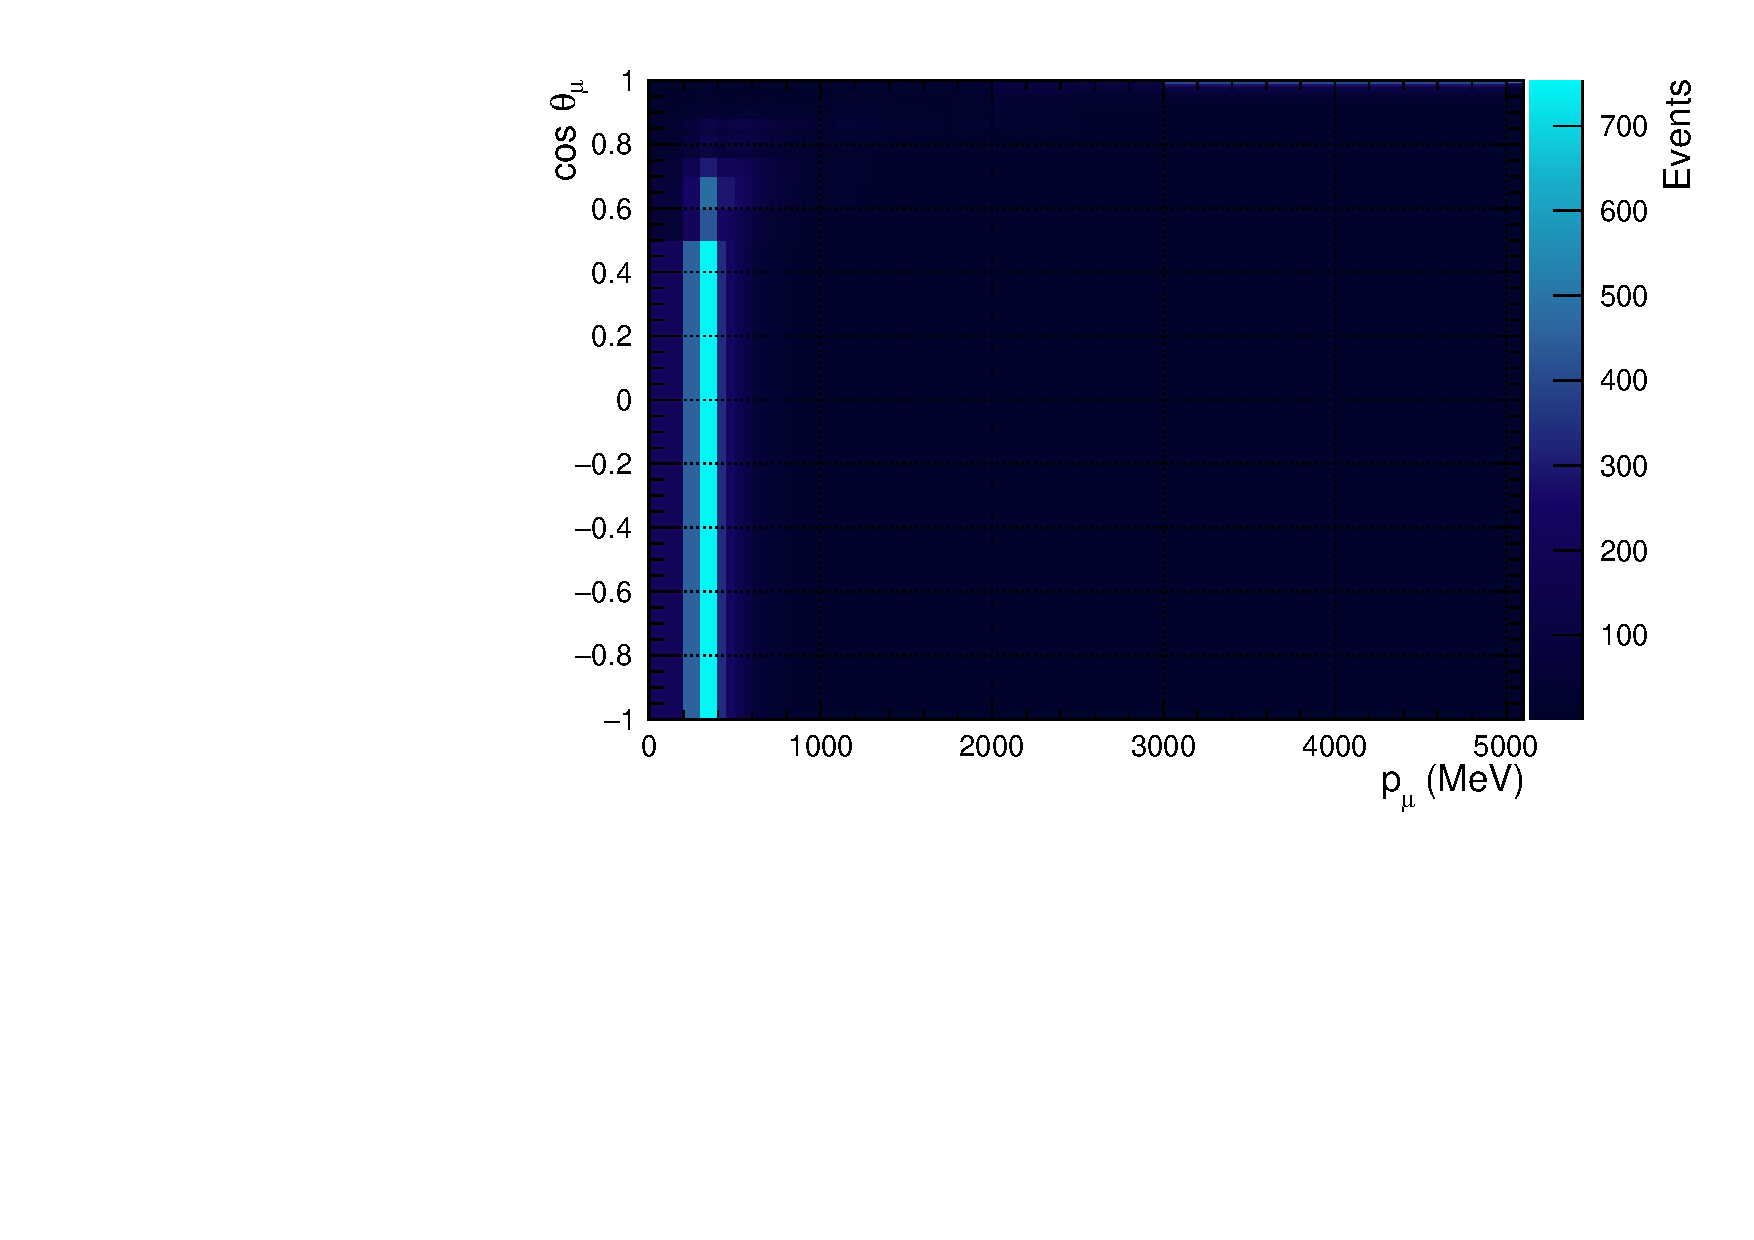
\includegraphics[width=0.95\linewidth]{figs/NomMC_MC_FGD1_numuCC_0pi}
  \caption{FGD1 FHC $\nu_{\mu}$ 0$\pi$}
  \label{fig:2d_FGD1_numuCC_0pi}
\end{subfigure}
\begin{subfigure}{.7\textwidth}
  \centering
  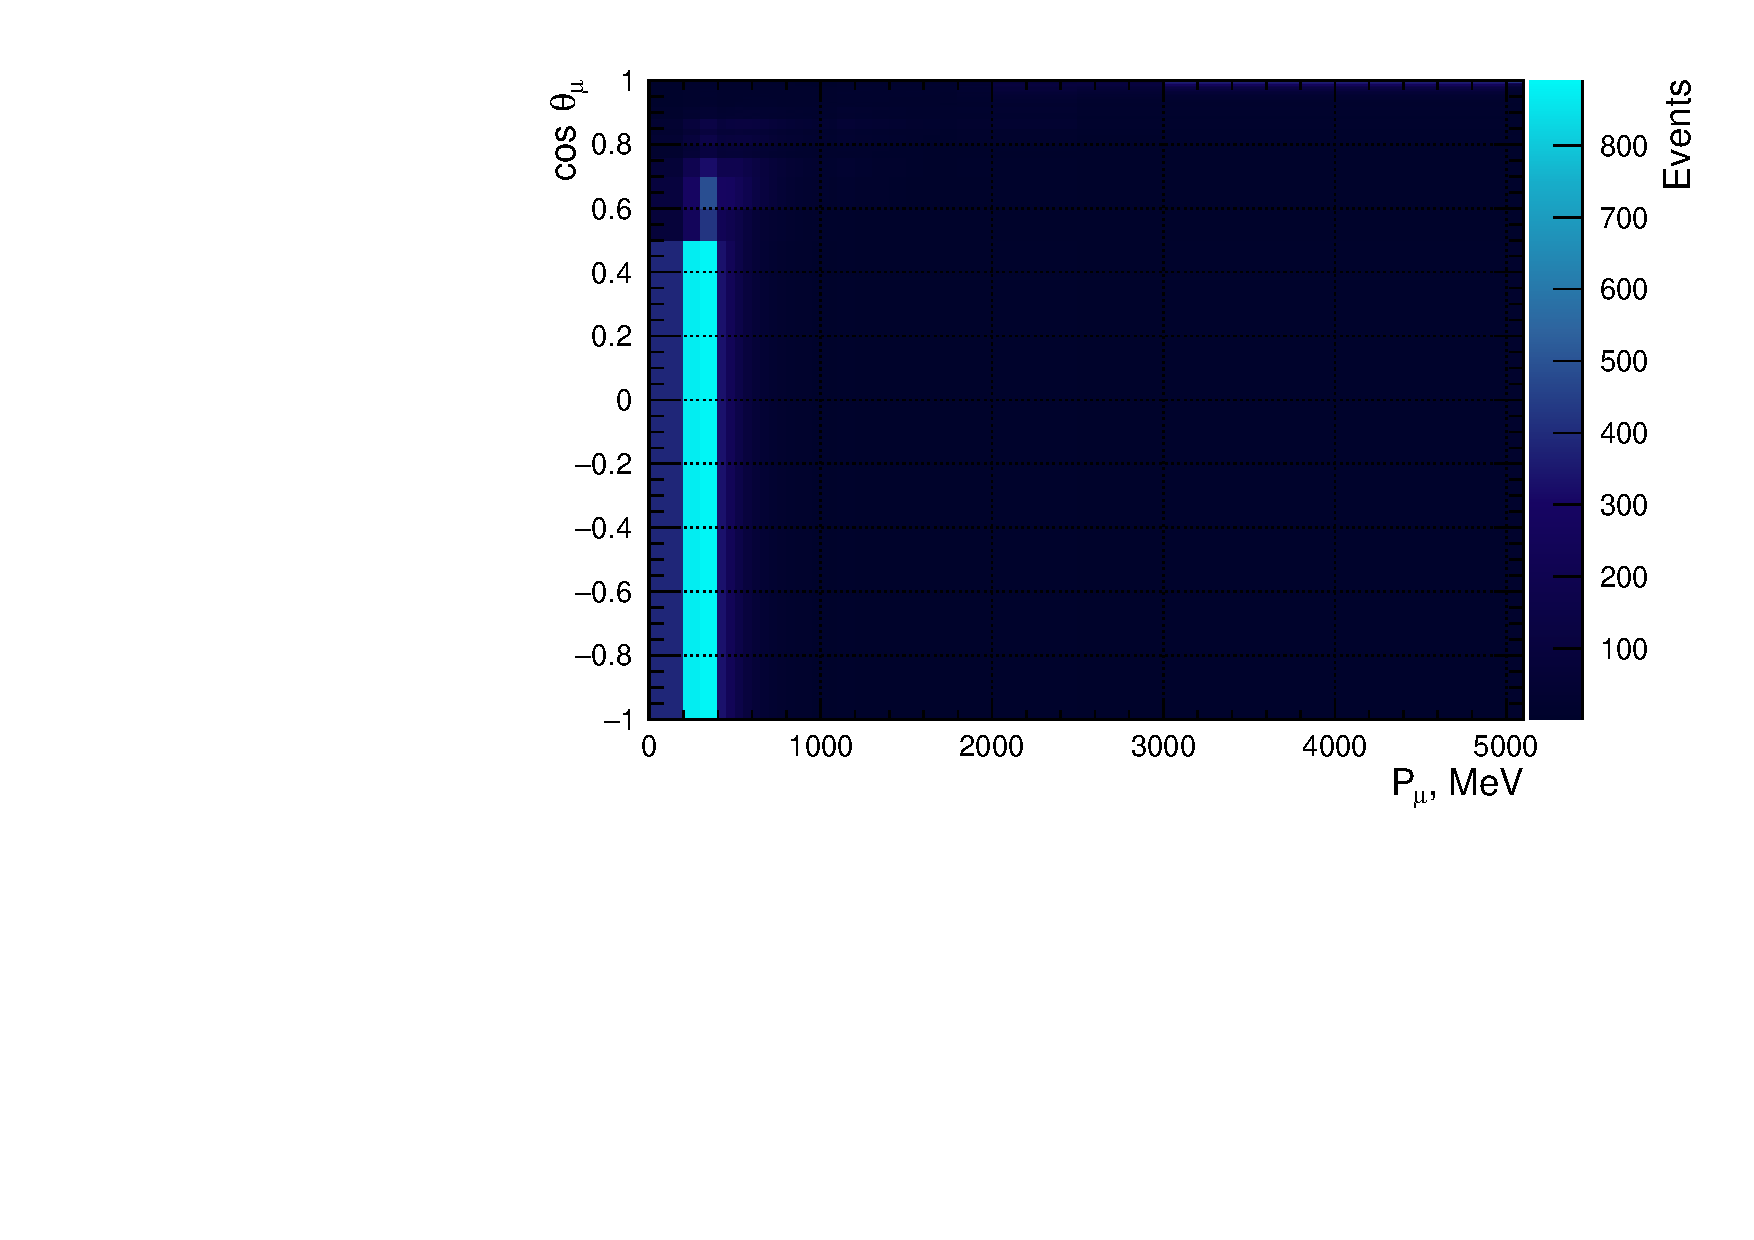
\includegraphics[width=0.95\linewidth]{figs/NomMC_MC_FGD2_numuCC_0pi}
  \caption{FGD2 FHC $\nu_{\mu}$ 0$\pi$}
  \label{fig:2d_FGD2_numuCC_0pi}
\end{subfigure}
\caption{Nominal MC distributions for the FGD1 and FGD2 CC-0$\pi$ samples. All samples are shown in Appendix \ref{app:nomMC}.}
\label{fig:2dnom}
\end{figure}

The projection of these distributions onto the $p_{\mu}$ axis are shown in Figure \ref{fig:pstack}, along with the data and interaction mode breakdown.

The CC 0$\pi$ and CC Other samples show oscillatory behaviour in the ratio of data to MC at low momentum. The ratio is consistently $>1$, but is slightly increased at the peak momentum for FHC and RHC $\nu$, and decreased at the peak for RHC $\bar{\nu}$. The ratio for the CC 1$\pi$ samples is more flat in momentum, but shows a small oscillation $<1$ at low momentum for FHC $\nu$, and $>1$ for RHC $\nu$ and $\bar{\nu}$. The behaviour is similar across the FGDs.

The FHC $\nu$ and RHC $\bar{\nu}$ CC 0$\pi$ samples are dominated by the target interaction modes CCQE and 2p2h. However, for RHC $\nu$, there is a large contamination of CC 1$\pi$ events. The FHC $\nu$ and RHC $\bar{\nu}$ CC 1$\pi$ samples are dominated by the target interaction modes CC 1$\pi$, CC coherent, and CC mult-$\pi$, but for RHC $\nu$, the 1$\pi$ sample has a significant number of CC DIS events. The CC Other samples are populated by mainly the target interaction modes CC DIS, CC mult-$\pi$, and CC miscellaneous, but with a significant number CC $1\pi$ and CC coherent events for FHC $\nu$ and RHC $\bar{\nu}$.

\begin{figure}[!h]
\centering
\begin{subfigure}{.24\textwidth}
  \centering
  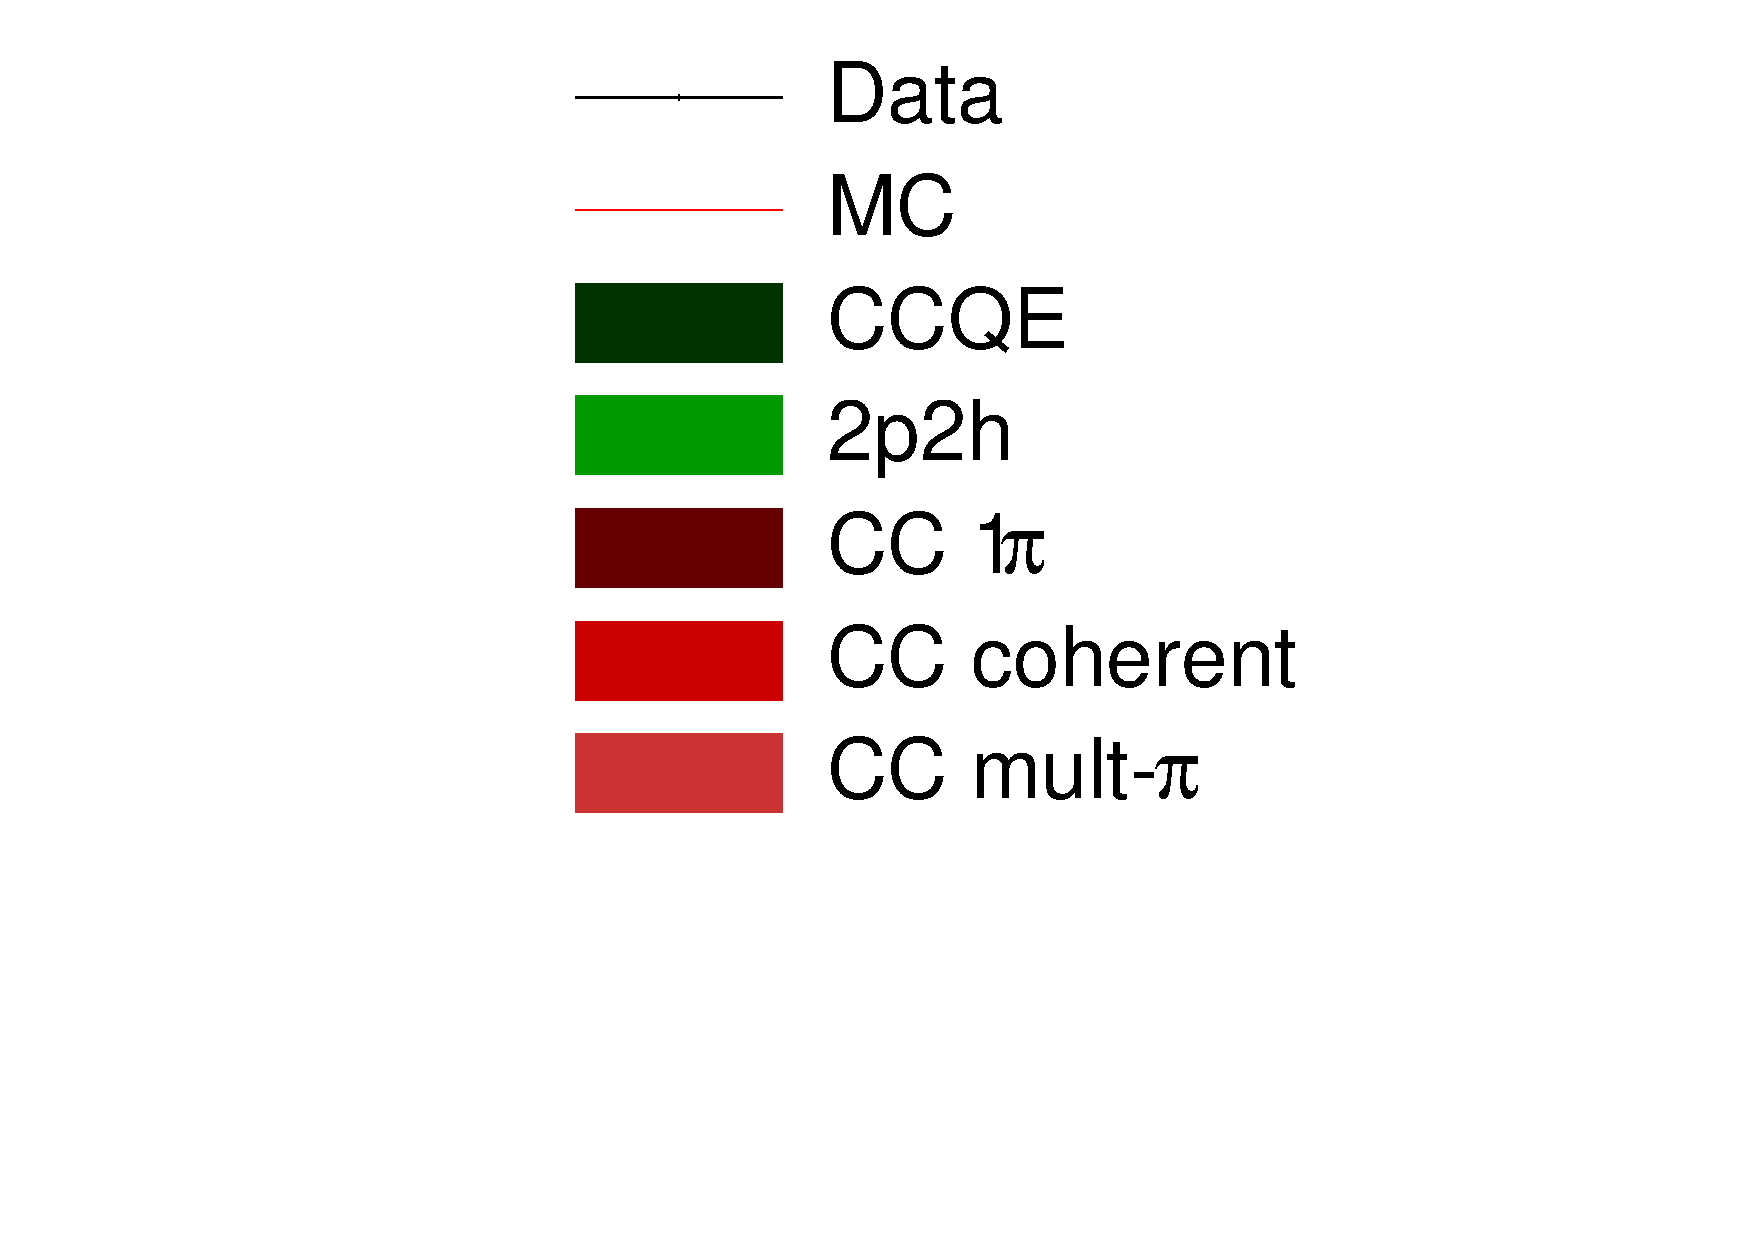
\includegraphics[width=\linewidth, trim={5mm 60mm 30mm 0mm}, clip]{figs/legend}
\end{subfigure}
\begin{subfigure}{.24\textwidth}
  \centering
  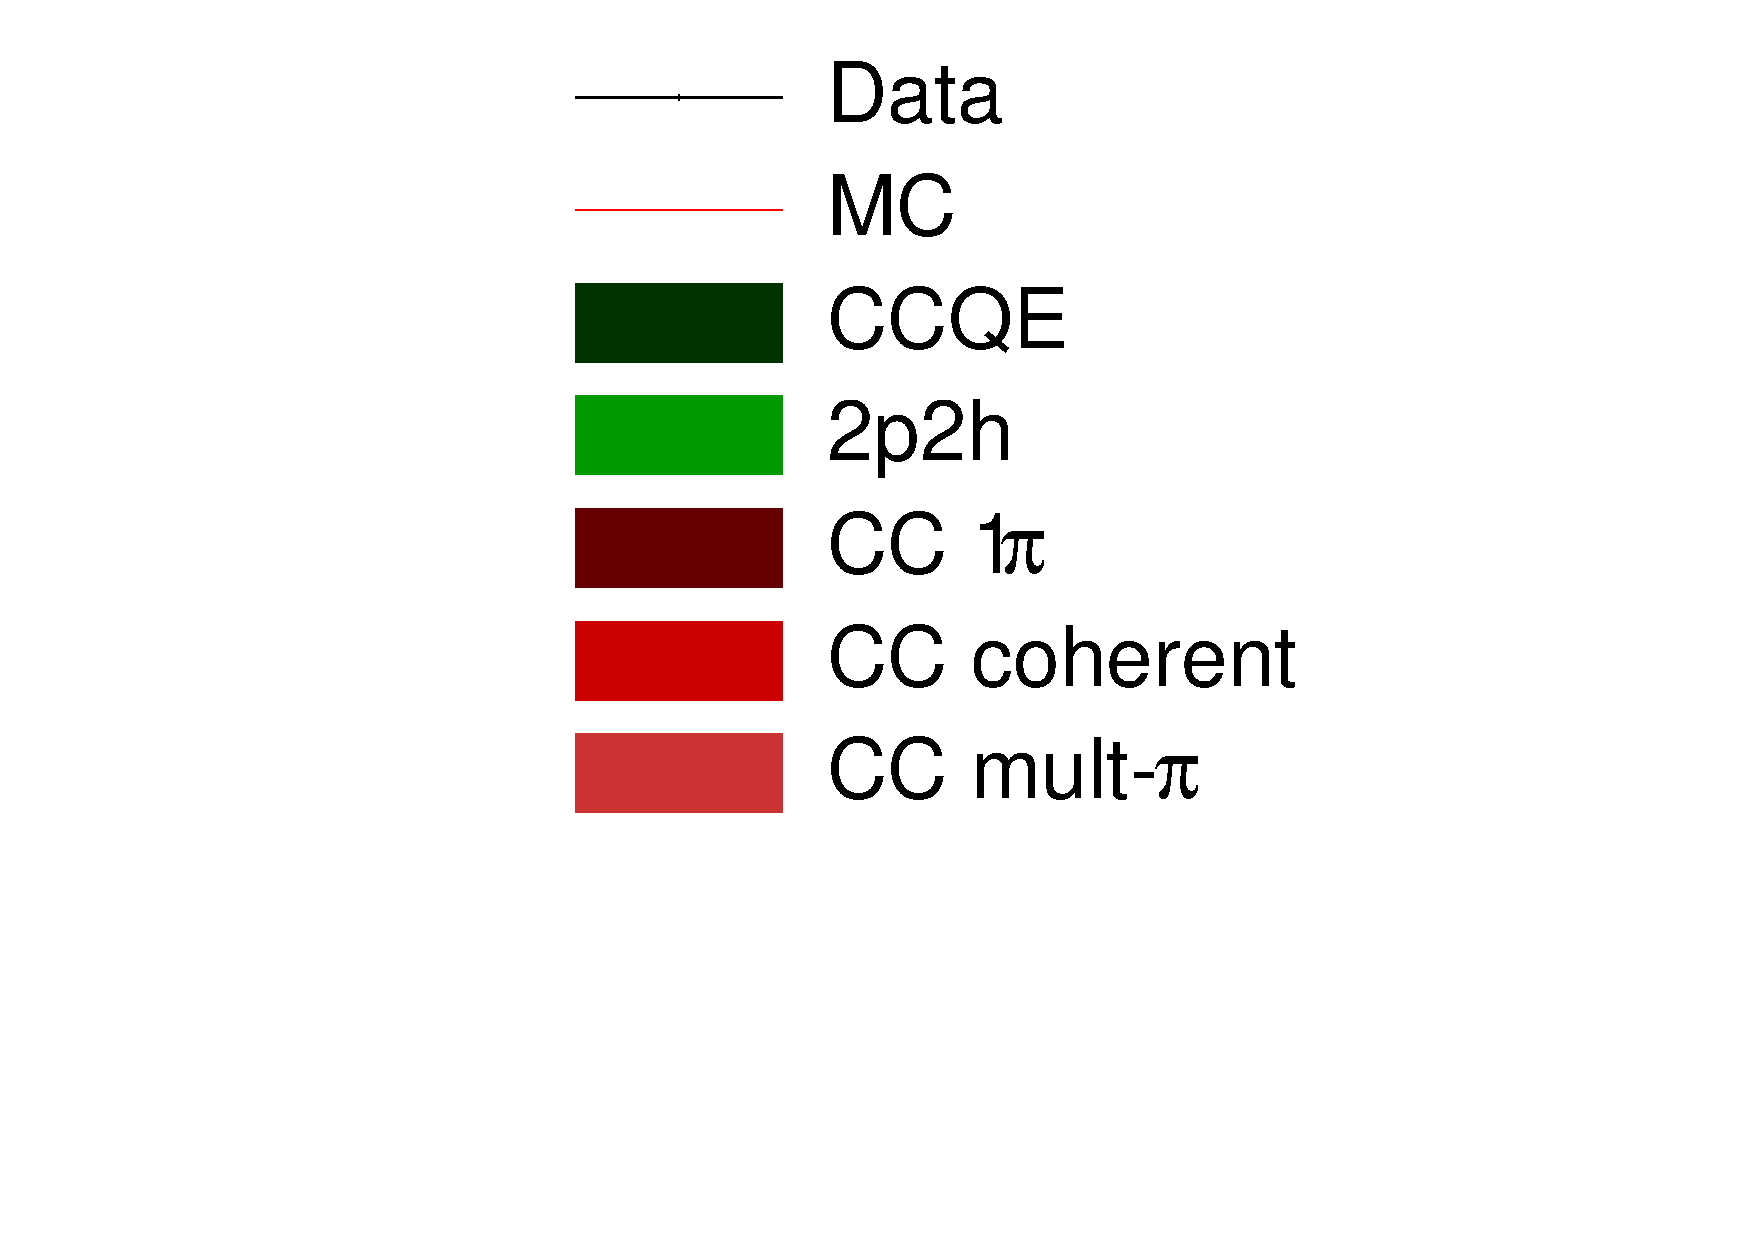
\includegraphics[width=\linewidth, trim={5mm 0mm 30mm 80mm}, clip]{figs/legend}
\end{subfigure}
\begin{subfigure}{.24\textwidth}
  \centering
  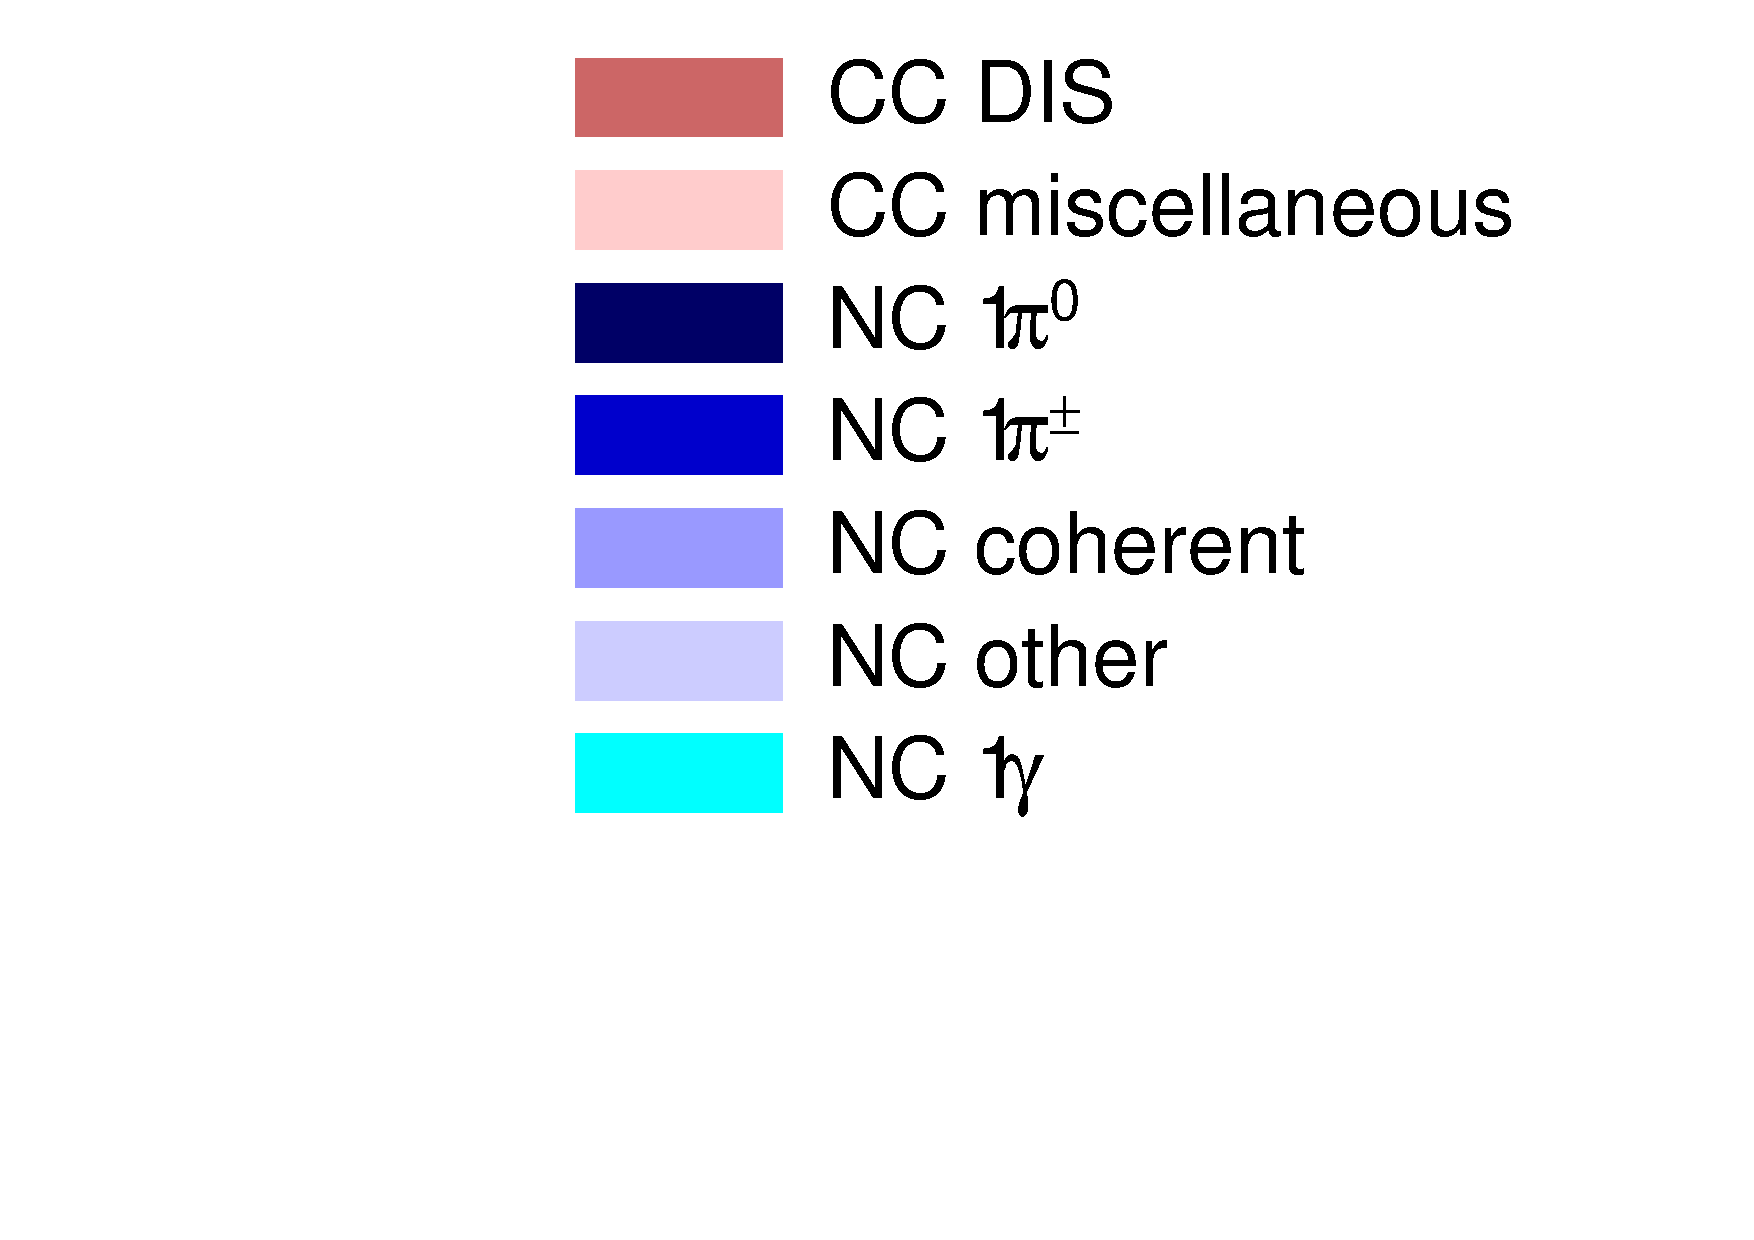
\includegraphics[width=\linewidth, trim={5mm 60mm 30mm 0mm}, clip]{figs/legend2}
\end{subfigure}
\begin{subfigure}{.24\textwidth}
  \centering
  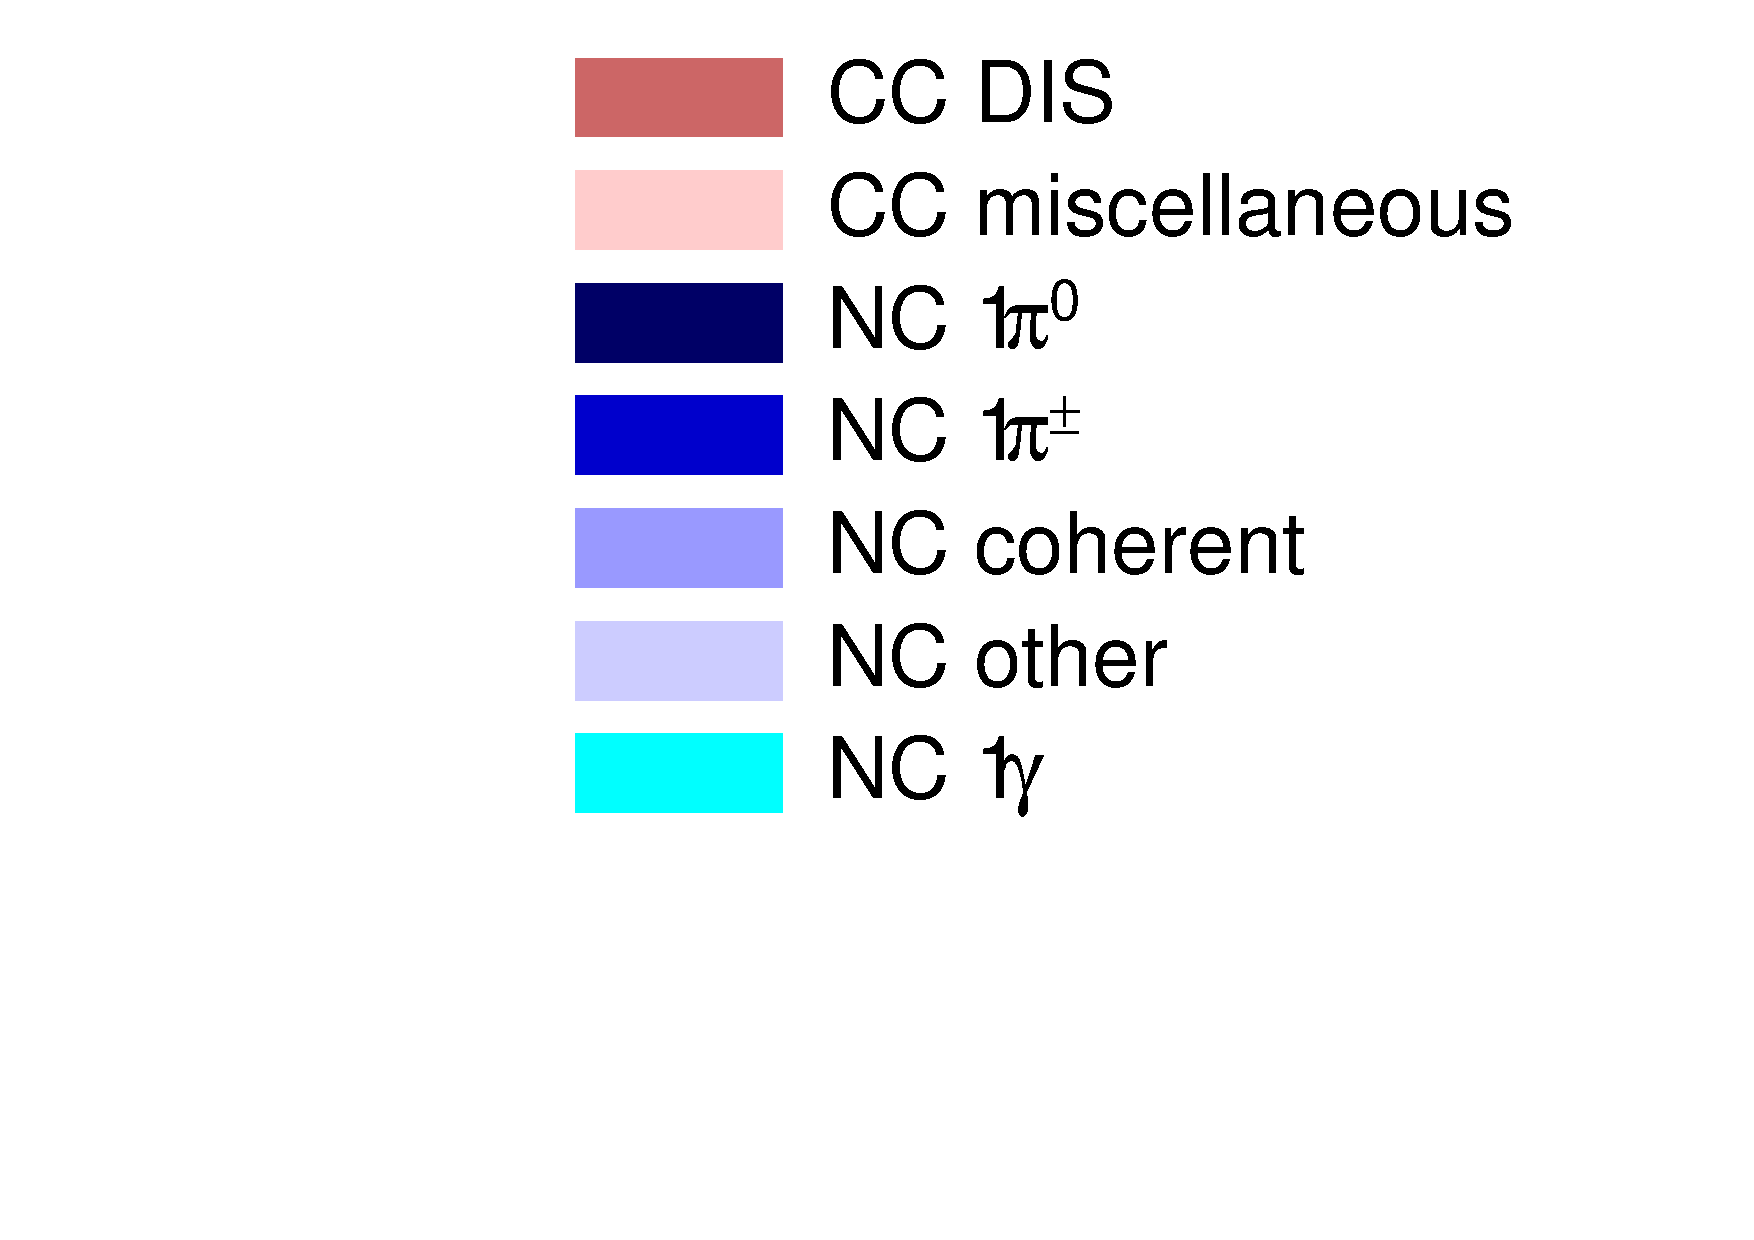
\includegraphics[width=\linewidth, trim={5mm 0mm 30mm 80mm}, clip]{figs/legend2}
\end{subfigure}

\begin{subfigure}{0.49\textwidth}
  \centering
  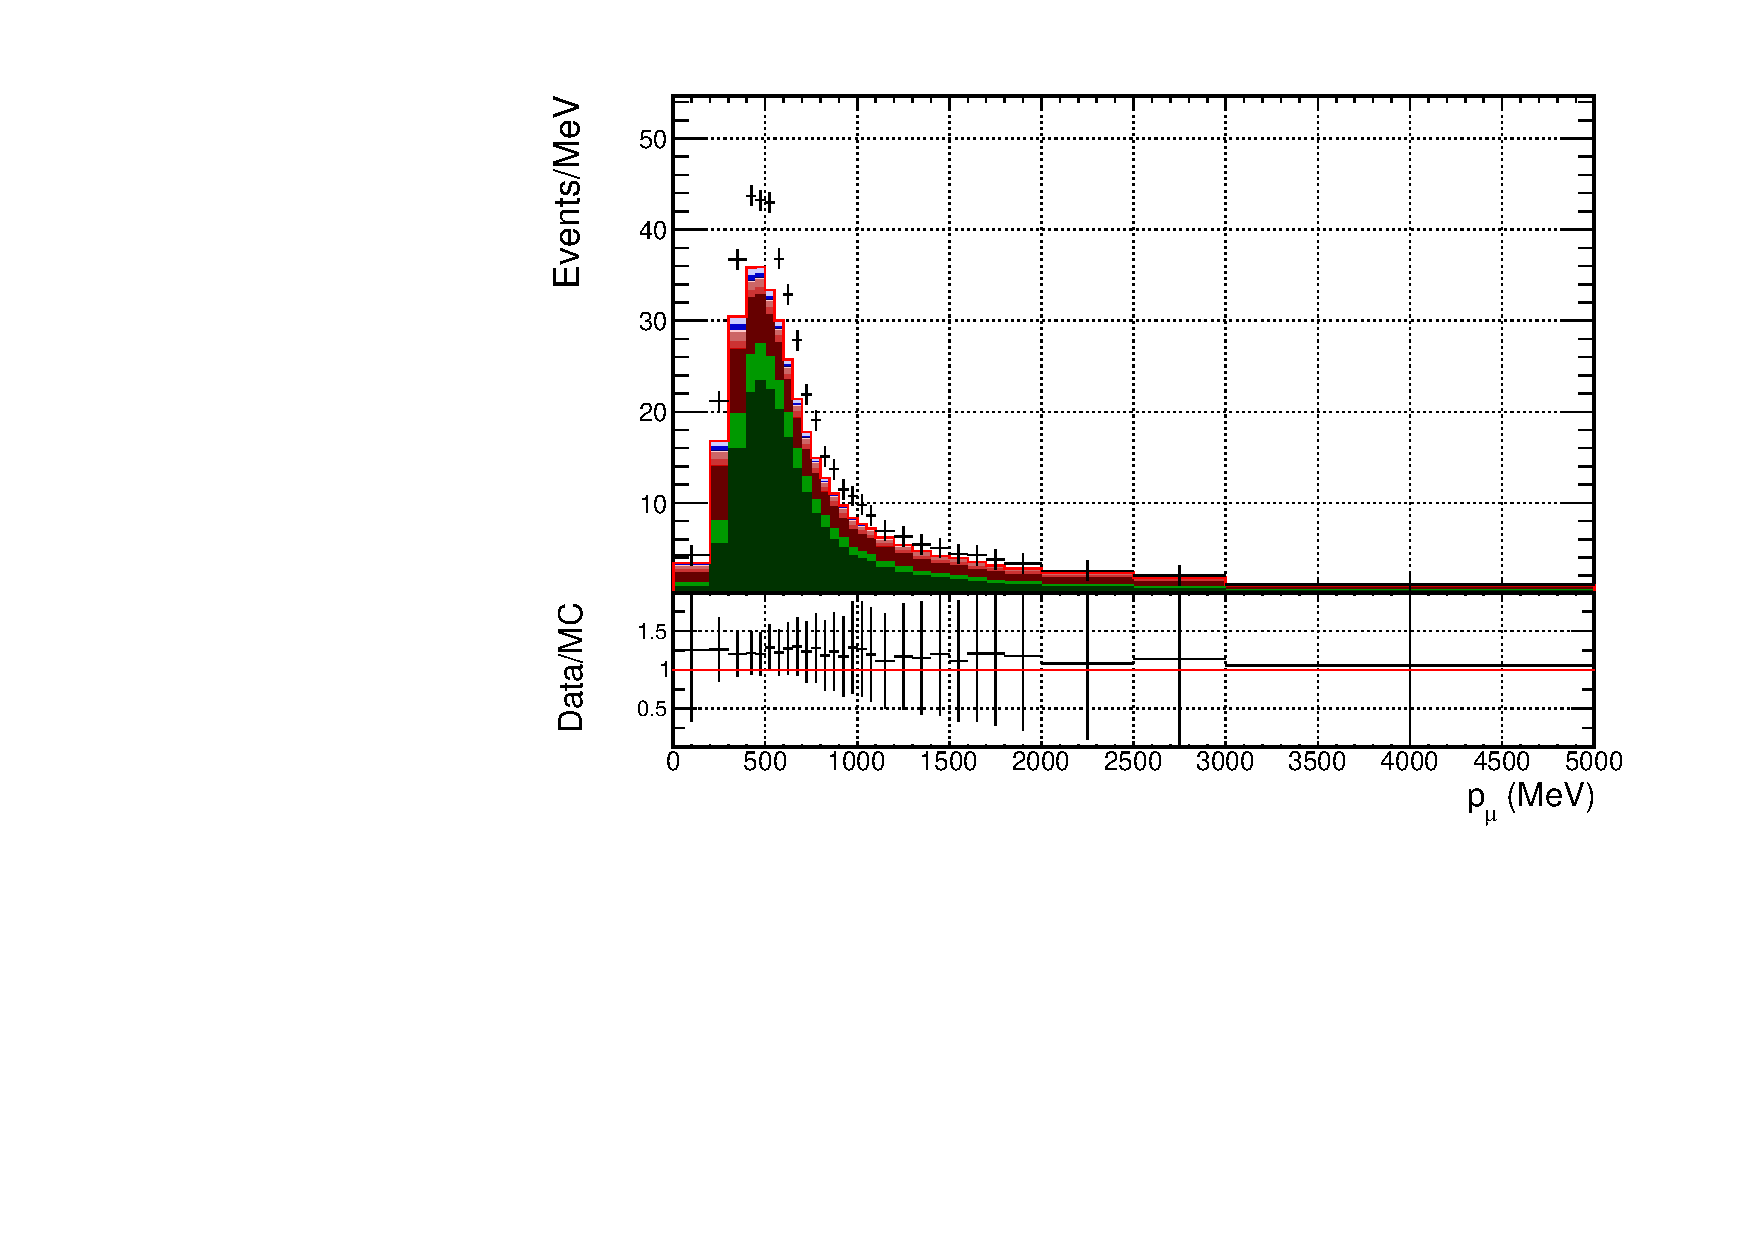
\includegraphics[width=\textwidth]{figs/FGD1_numuCC_0pi_p}
  \caption{FGD1 FHC $\nu_{\mu}$ 0$\pi$}
\end{subfigure}
\begin{subfigure}{0.49\textwidth}
  \centering
  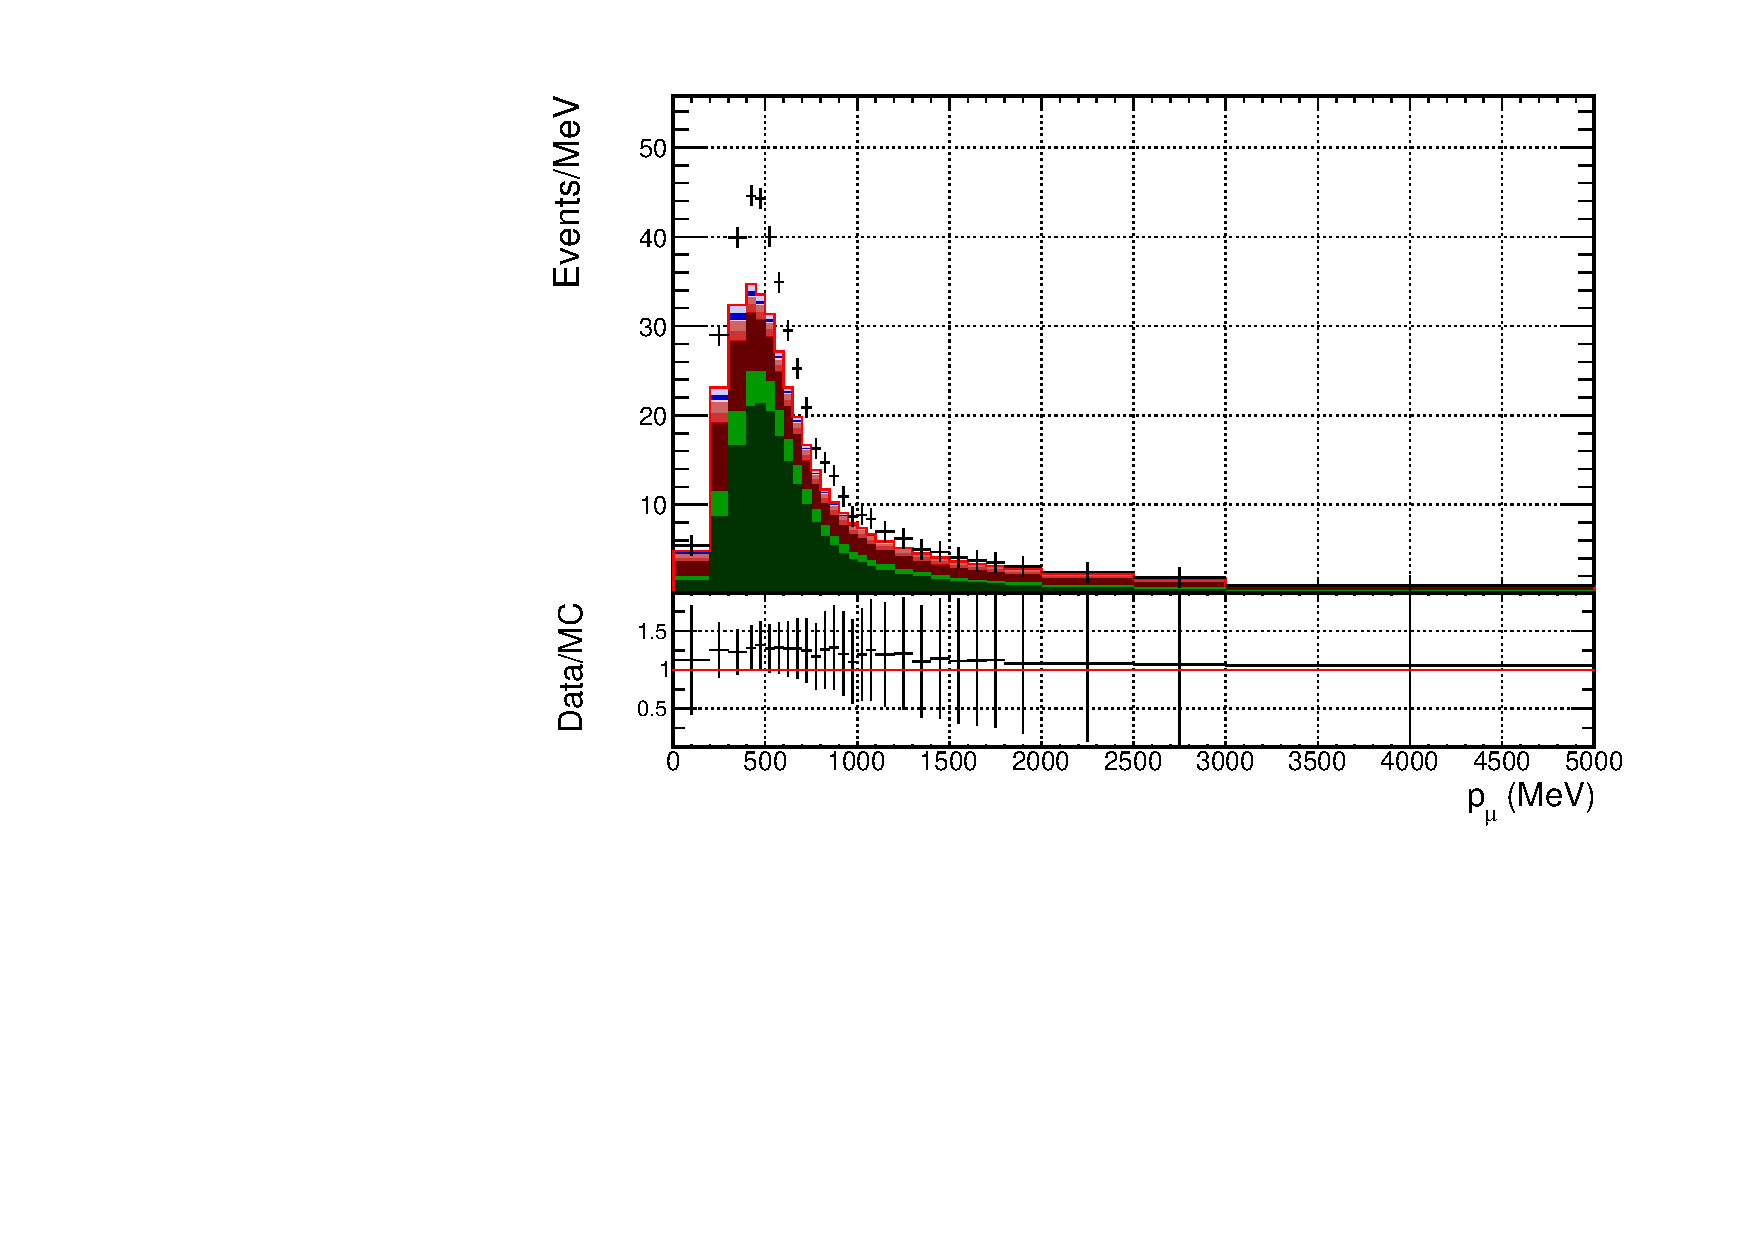
\includegraphics[width=\textwidth]{figs/FGD2_numuCC_0pi_p}
  \caption{FGD2 FHC $\nu_{\mu}$ 0$\pi$}
\end{subfigure}

\begin{subfigure}{0.49\textwidth}
  \centering
  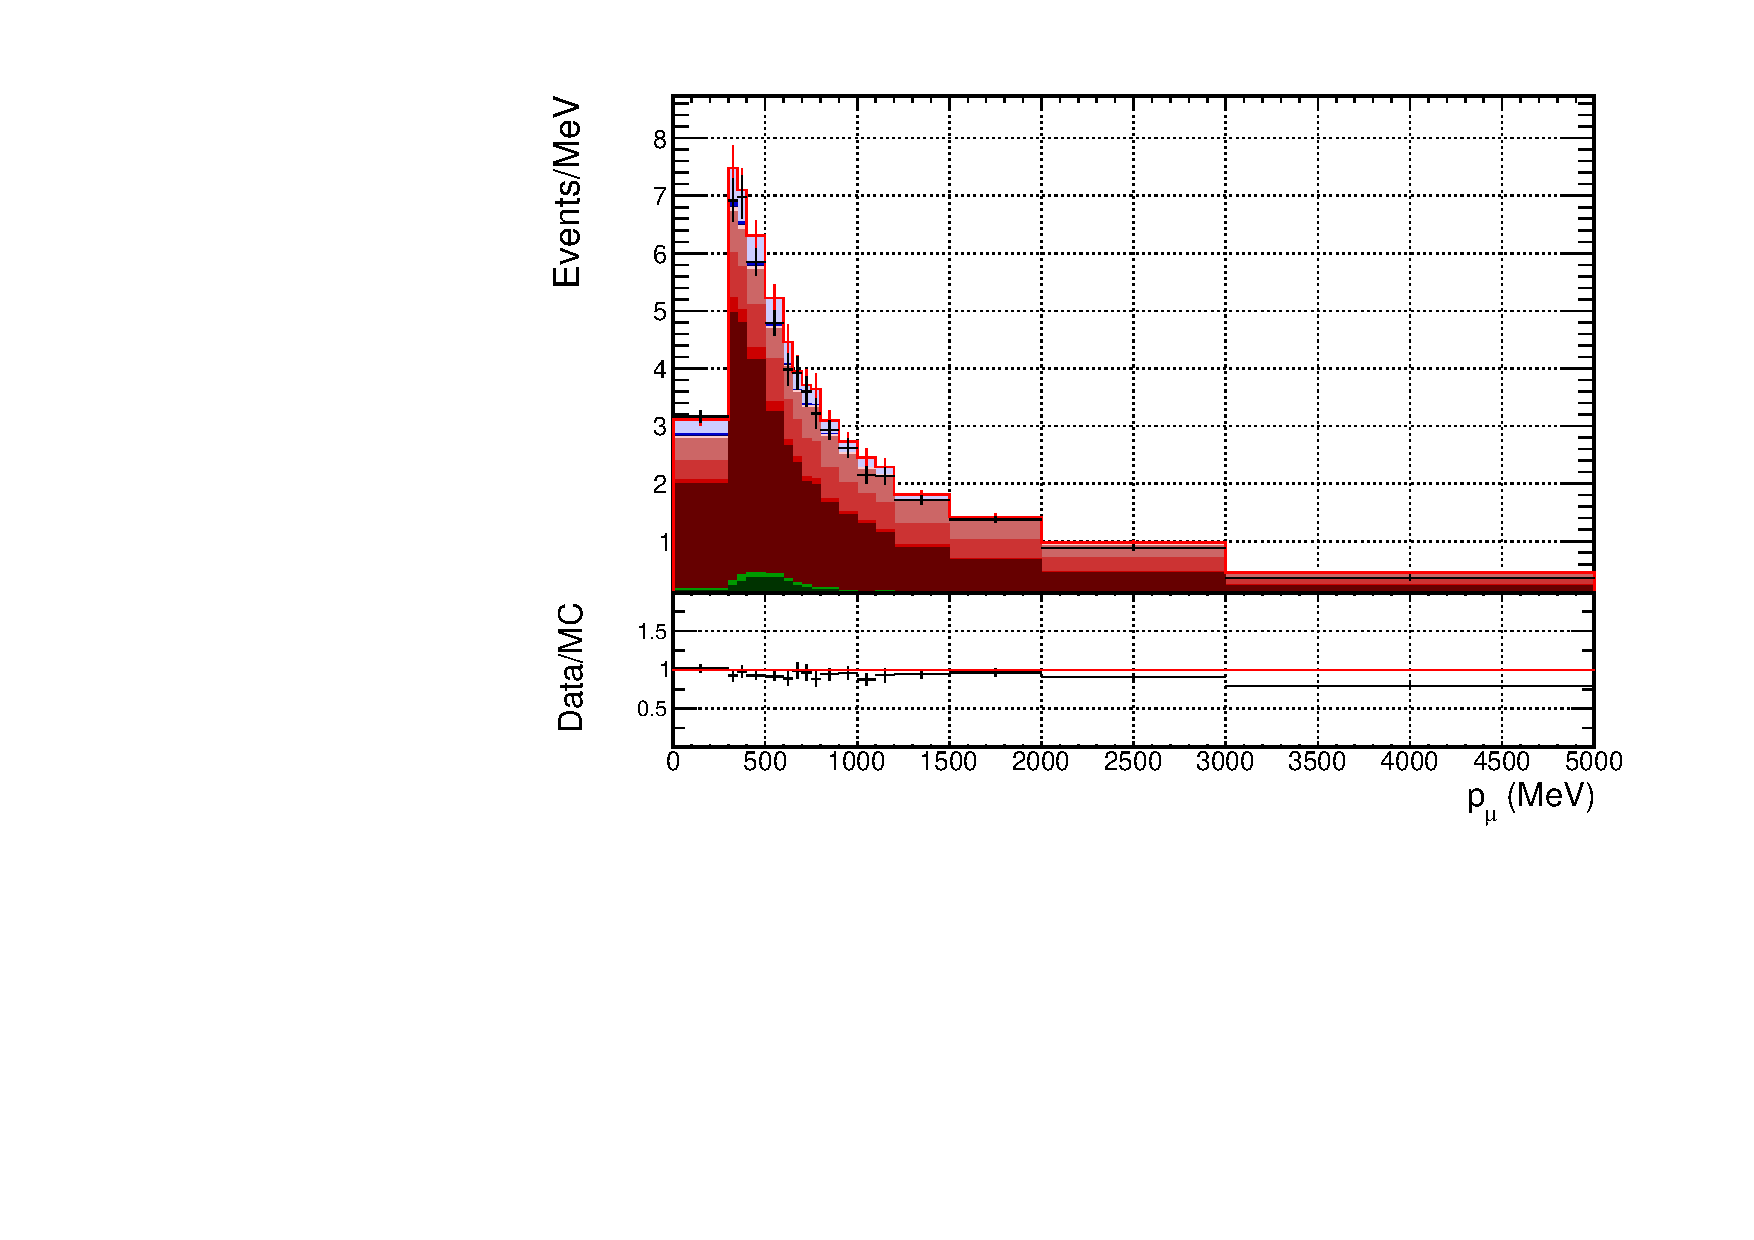
\includegraphics[width=\textwidth]{figs/FGD1_numuCC_1pi_p}
  \caption{FGD1 FHC $\nu_{\mu}$  1$\pi$}
\end{subfigure}
\begin{subfigure}{0.49\textwidth}
  \centering
  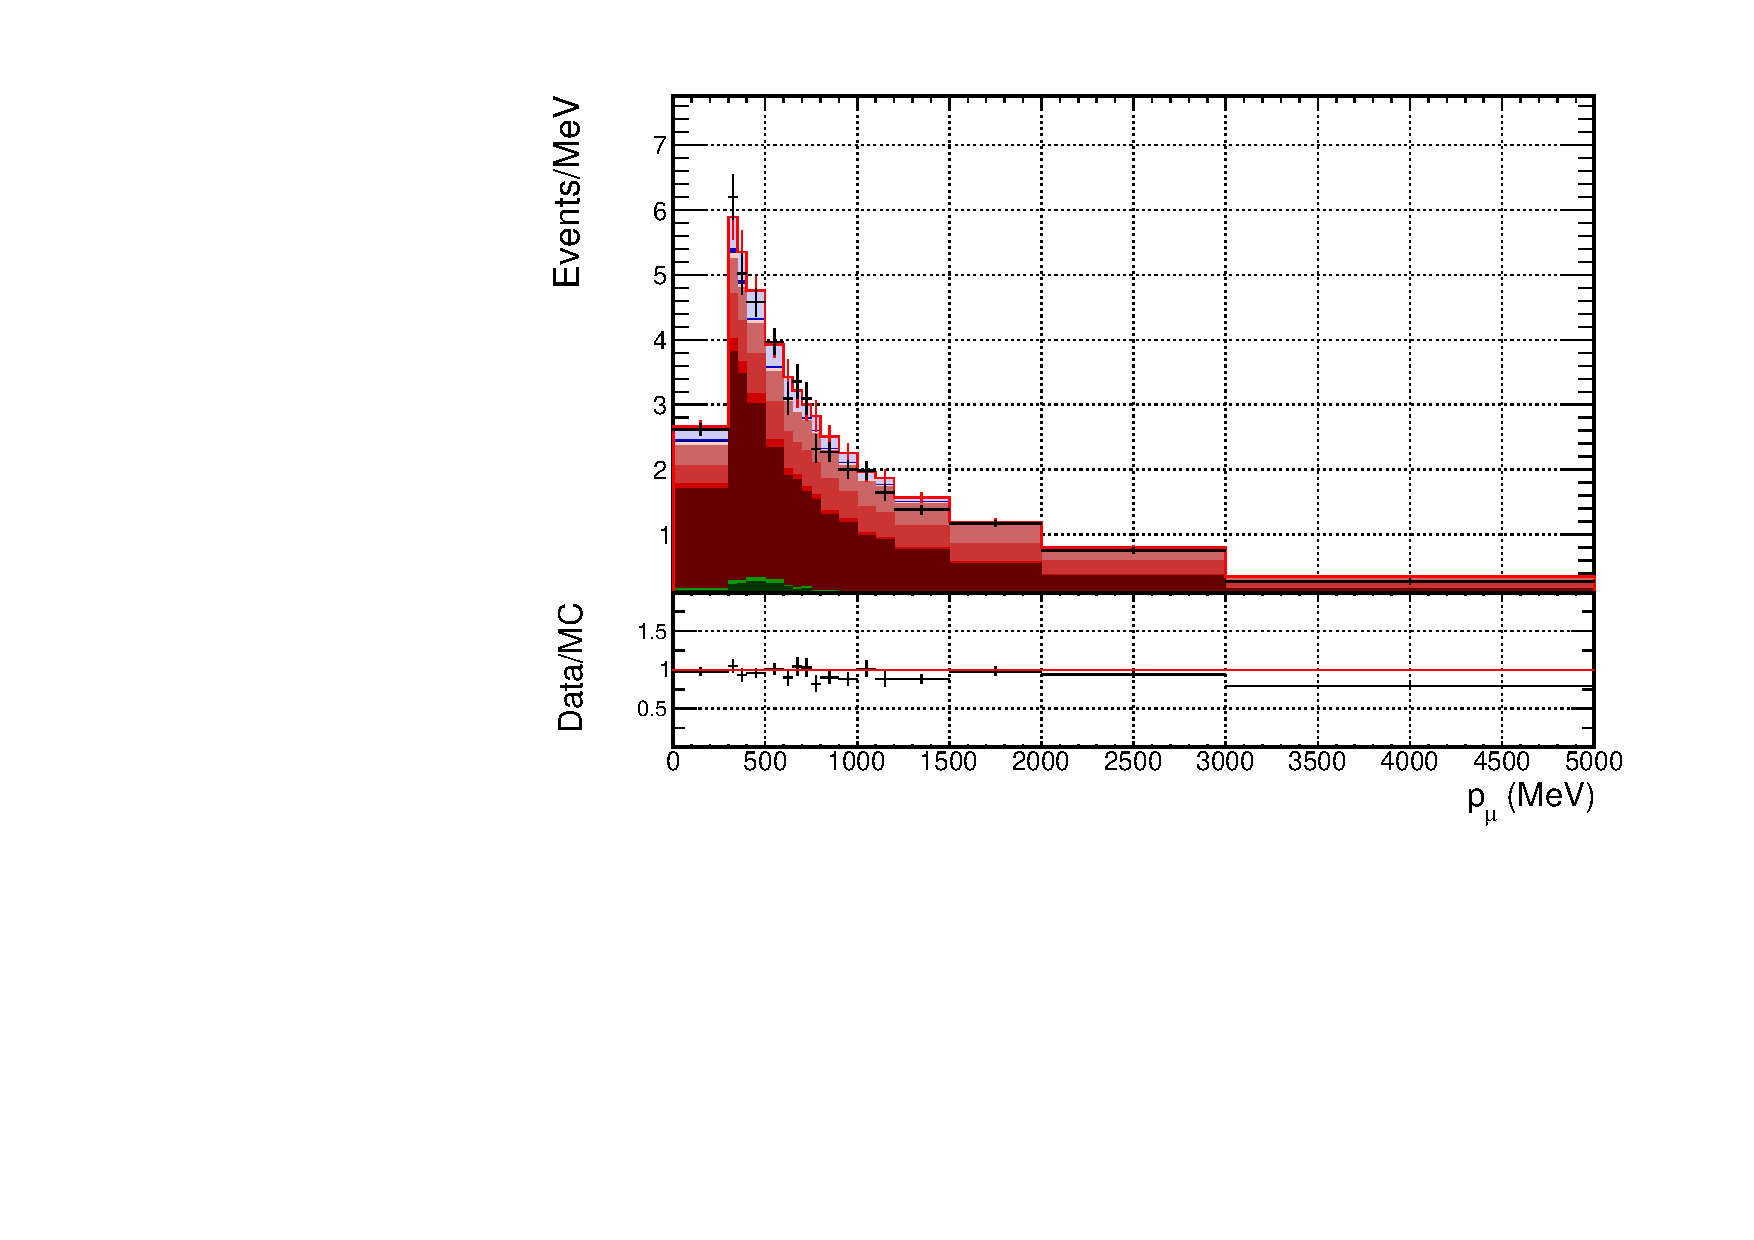
\includegraphics[width=\textwidth]{figs/FGD2_numuCC_1pi_p}
  \caption{FGD2 FHC $\nu_{\mu}$ 1$\pi$}
\end{subfigure}

\begin{subfigure}{0.49\textwidth}
  \centering
  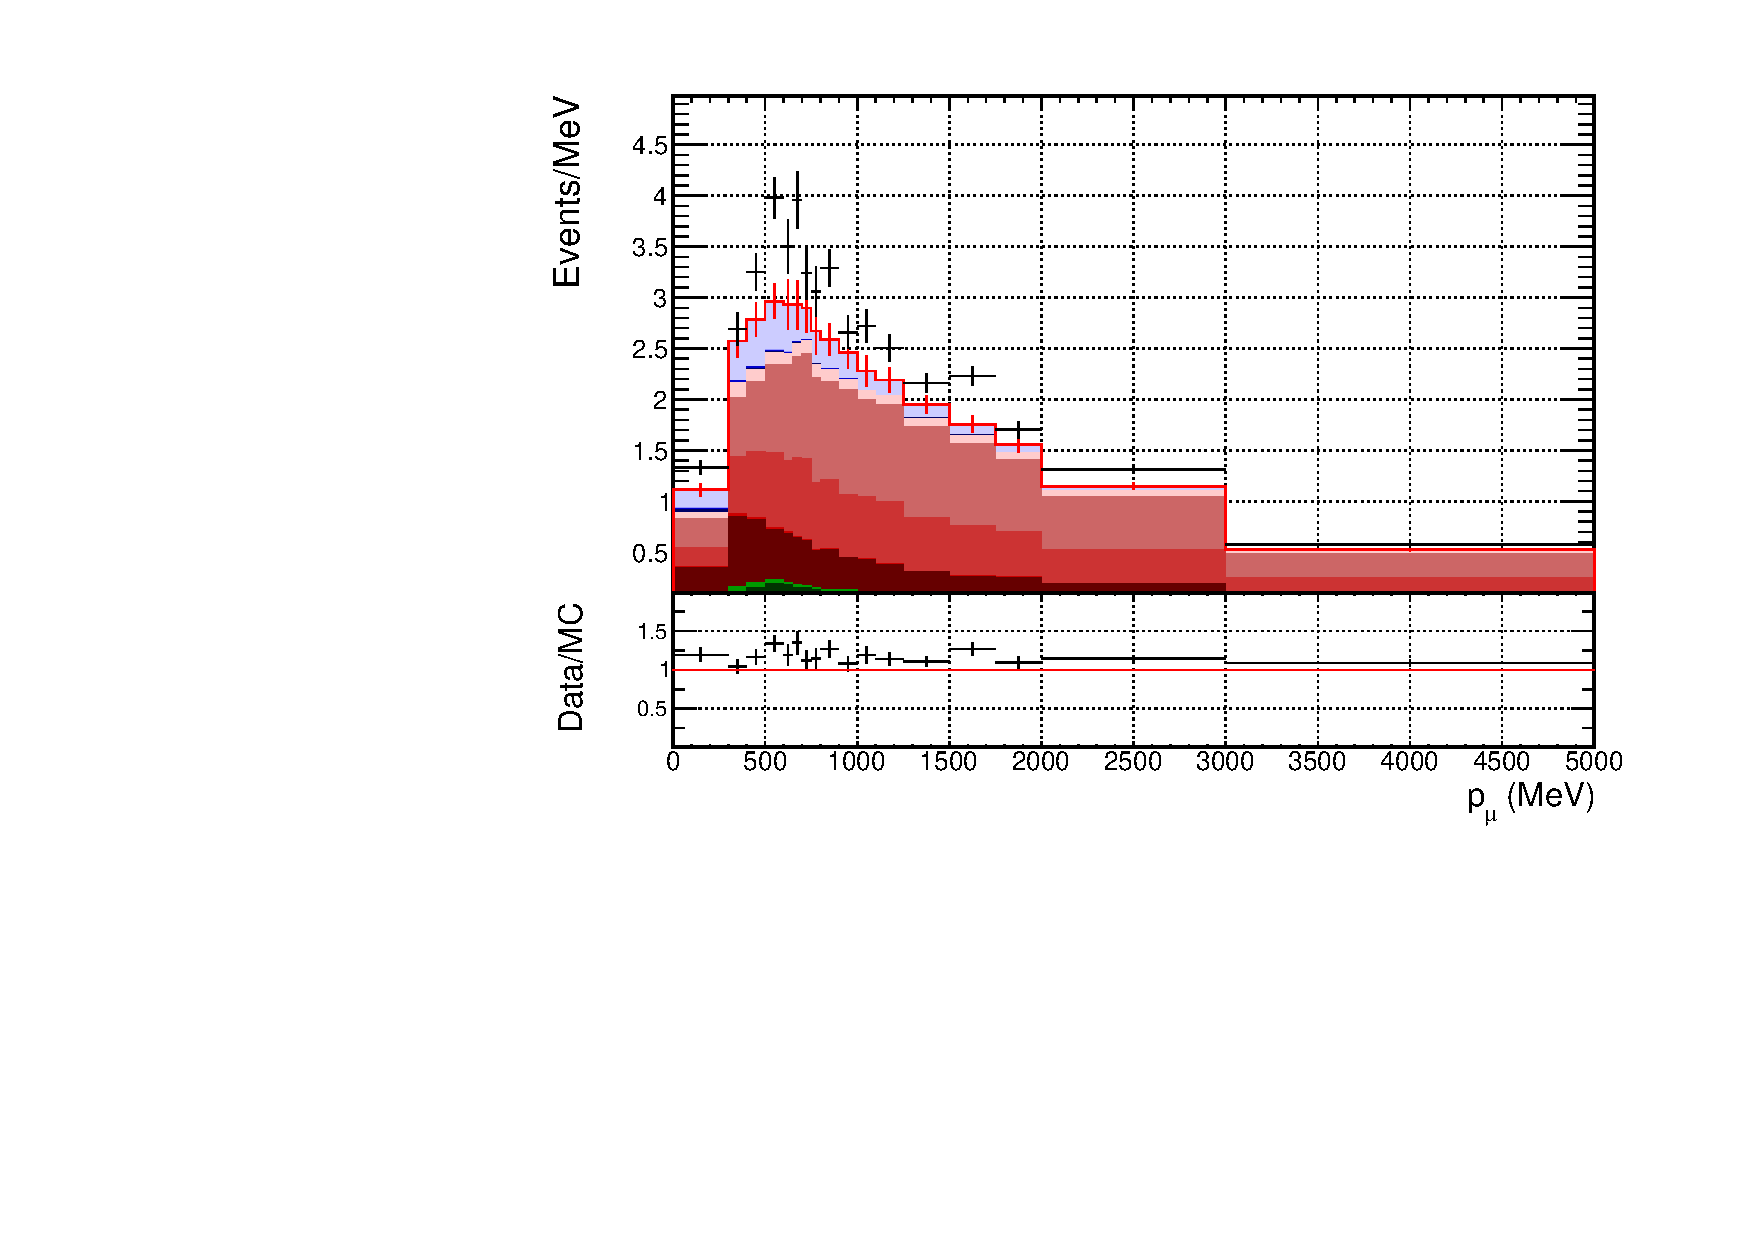
\includegraphics[width=\textwidth]{figs/FGD1_numuCC_other_p}
  \caption{FGD1 FHC $\nu_{\mu}$ Other}
\end{subfigure}
\begin{subfigure}{0.49\textwidth}
  \centering
  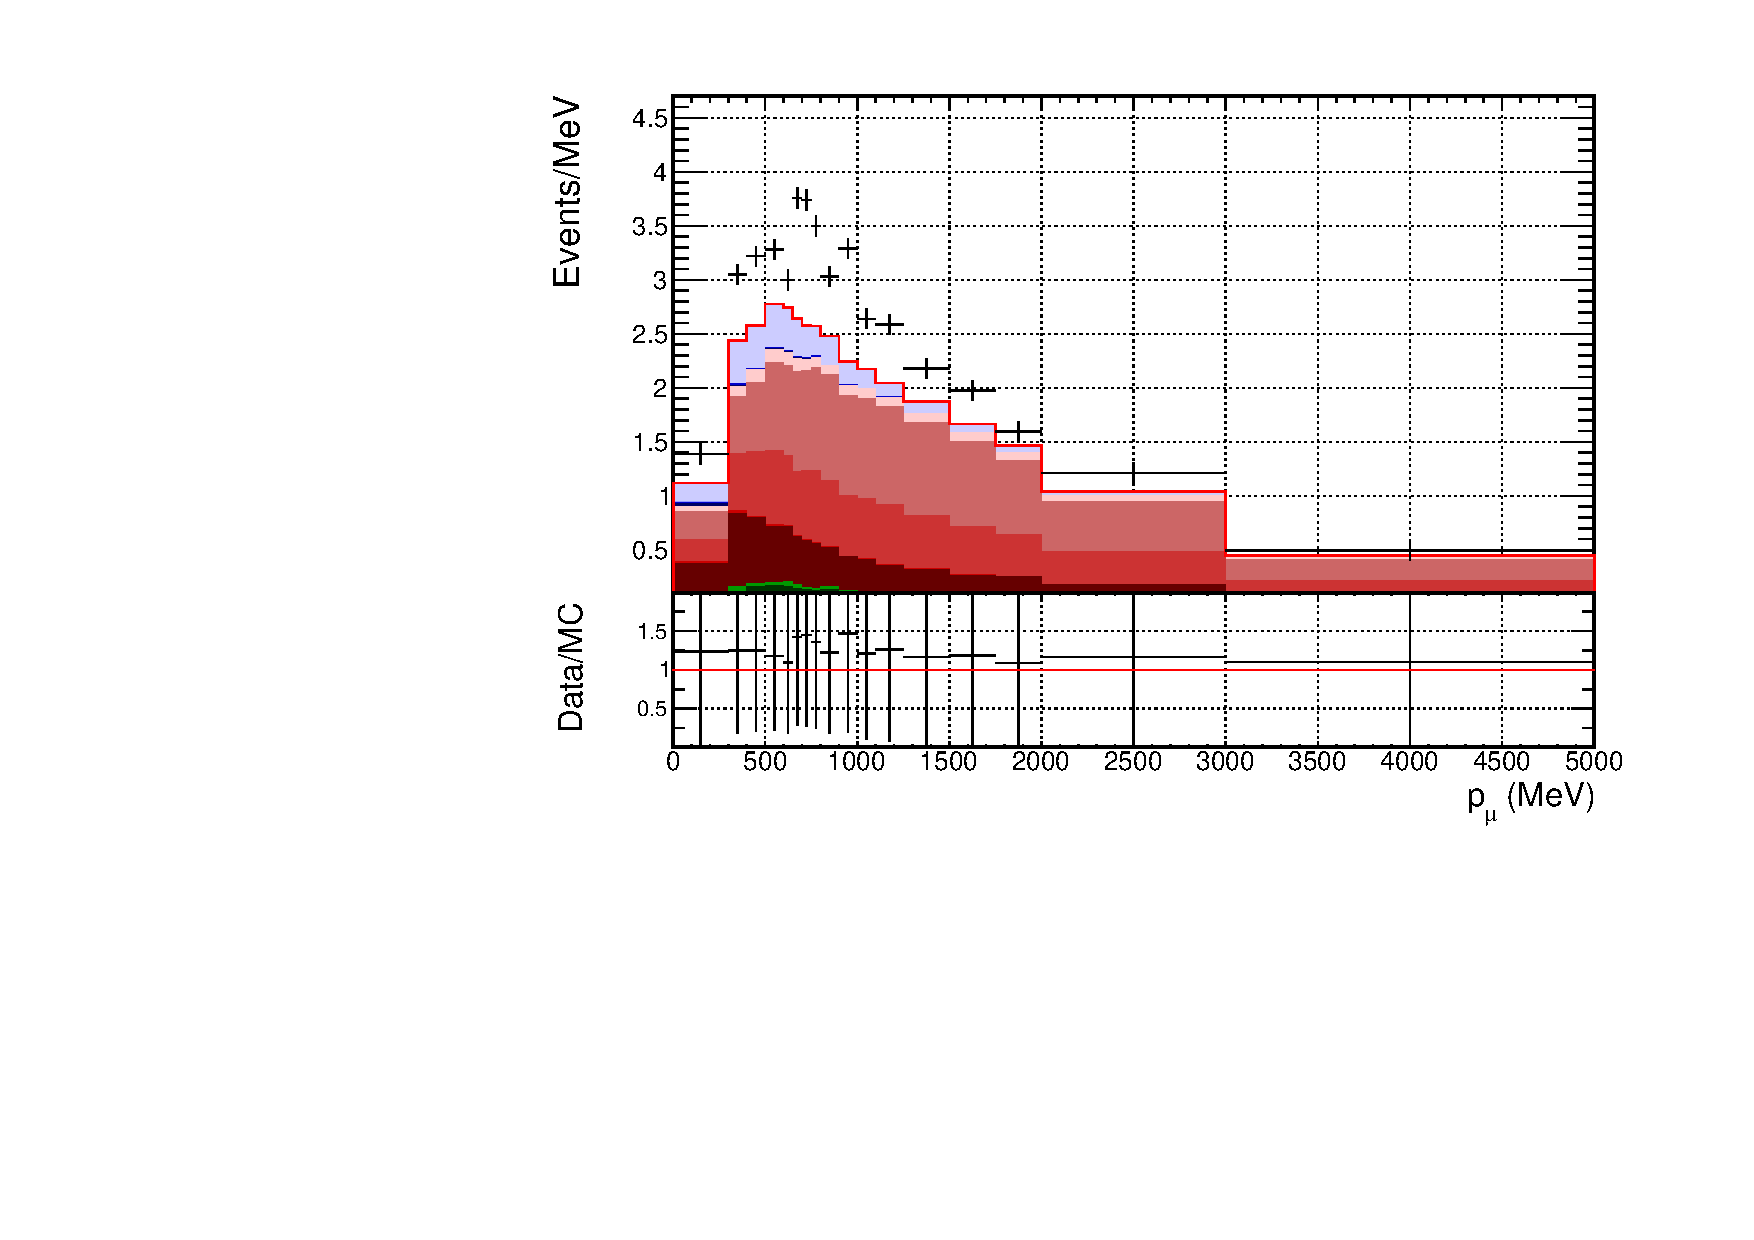
\includegraphics[width=\textwidth]{figs/FGD2_numuCC_other_p}
  \caption{FGD2 FHC $\nu_{\mu}$ Other}
\end{subfigure}
\caption{$p_{\mu}$ projections of data and nominal MC broken down by interaction mode for FHC selections.}
\label{fig:pstack_fhc}
\end{figure}

\begin{figure}[!h]
\centering
\begin{subfigure}{.24\textwidth}
  \centering
  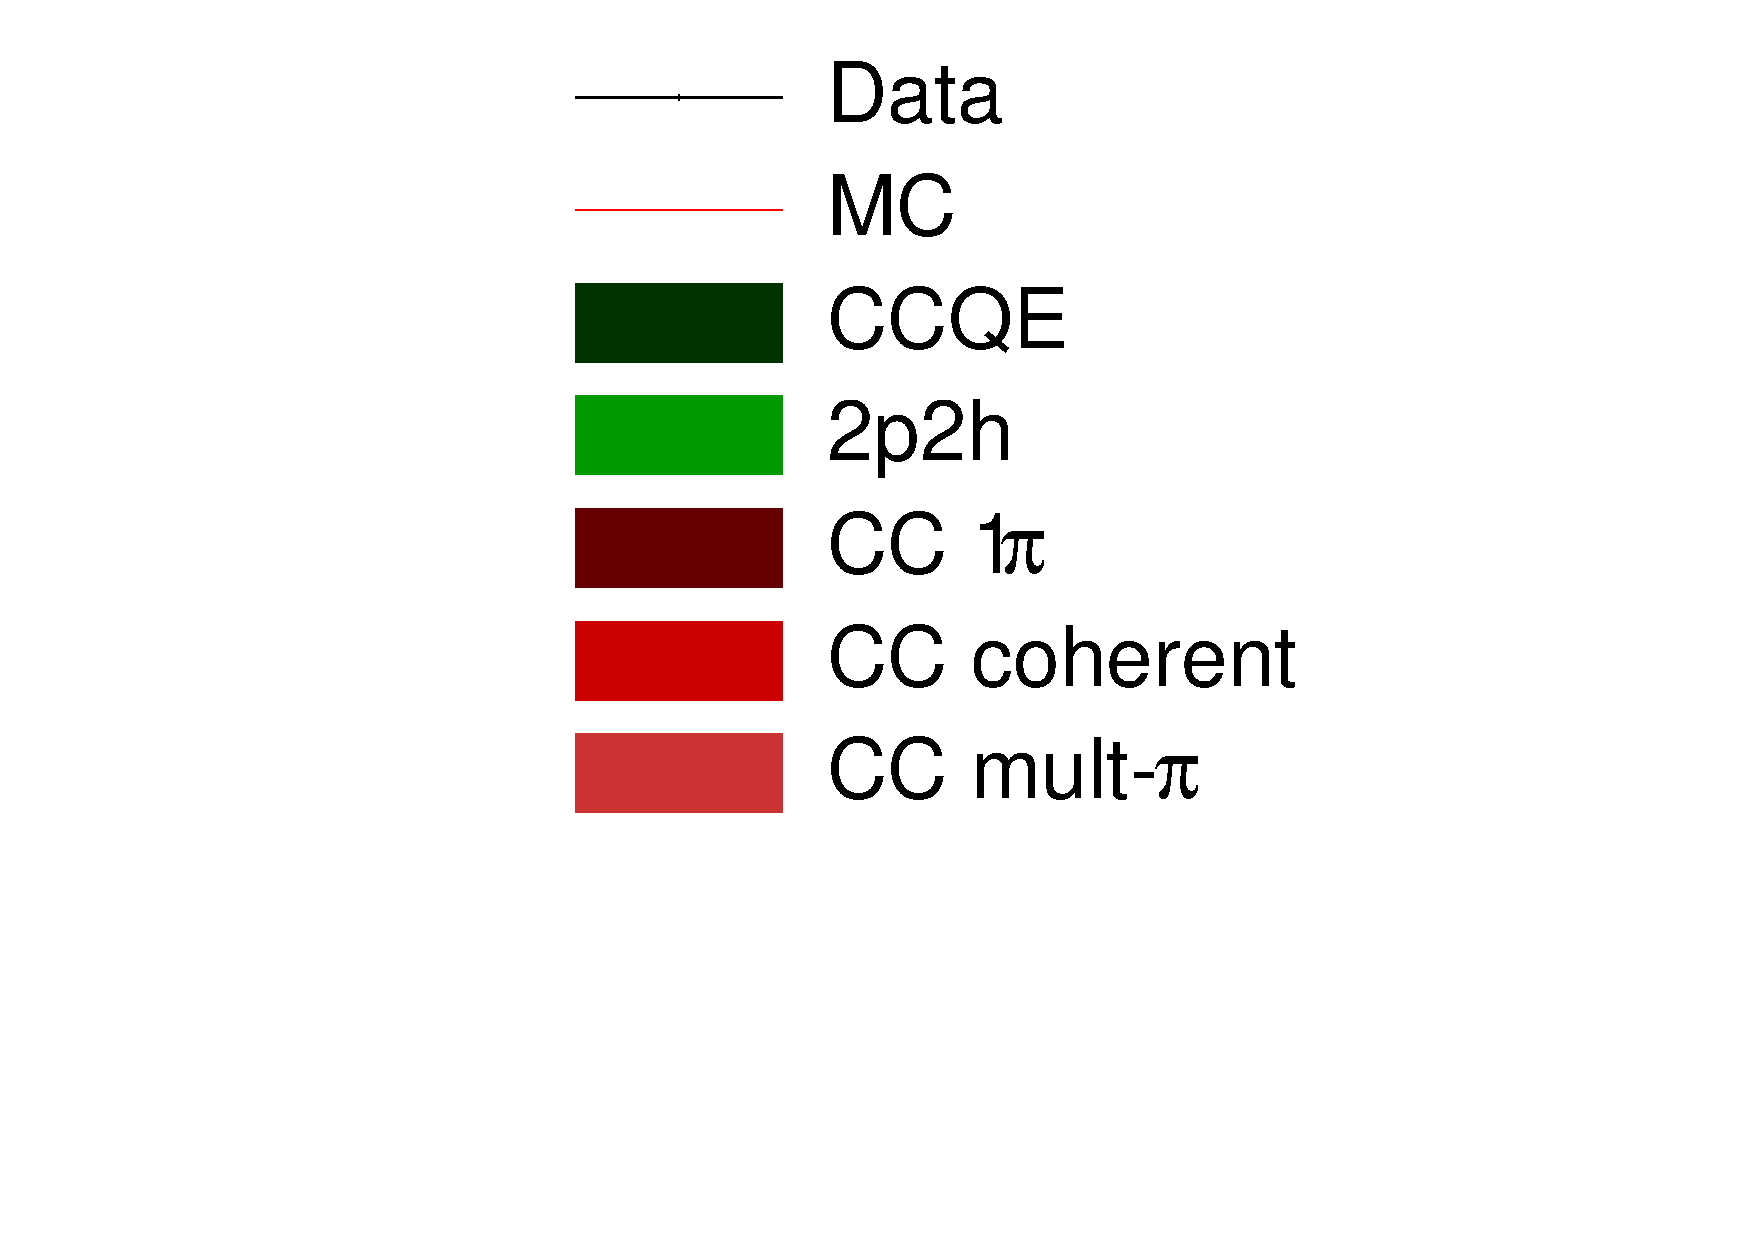
\includegraphics[width=\linewidth, trim={5mm 60mm 30mm 0mm}, clip]{figs/legend}
\end{subfigure}
\begin{subfigure}{.24\textwidth}
  \centering
  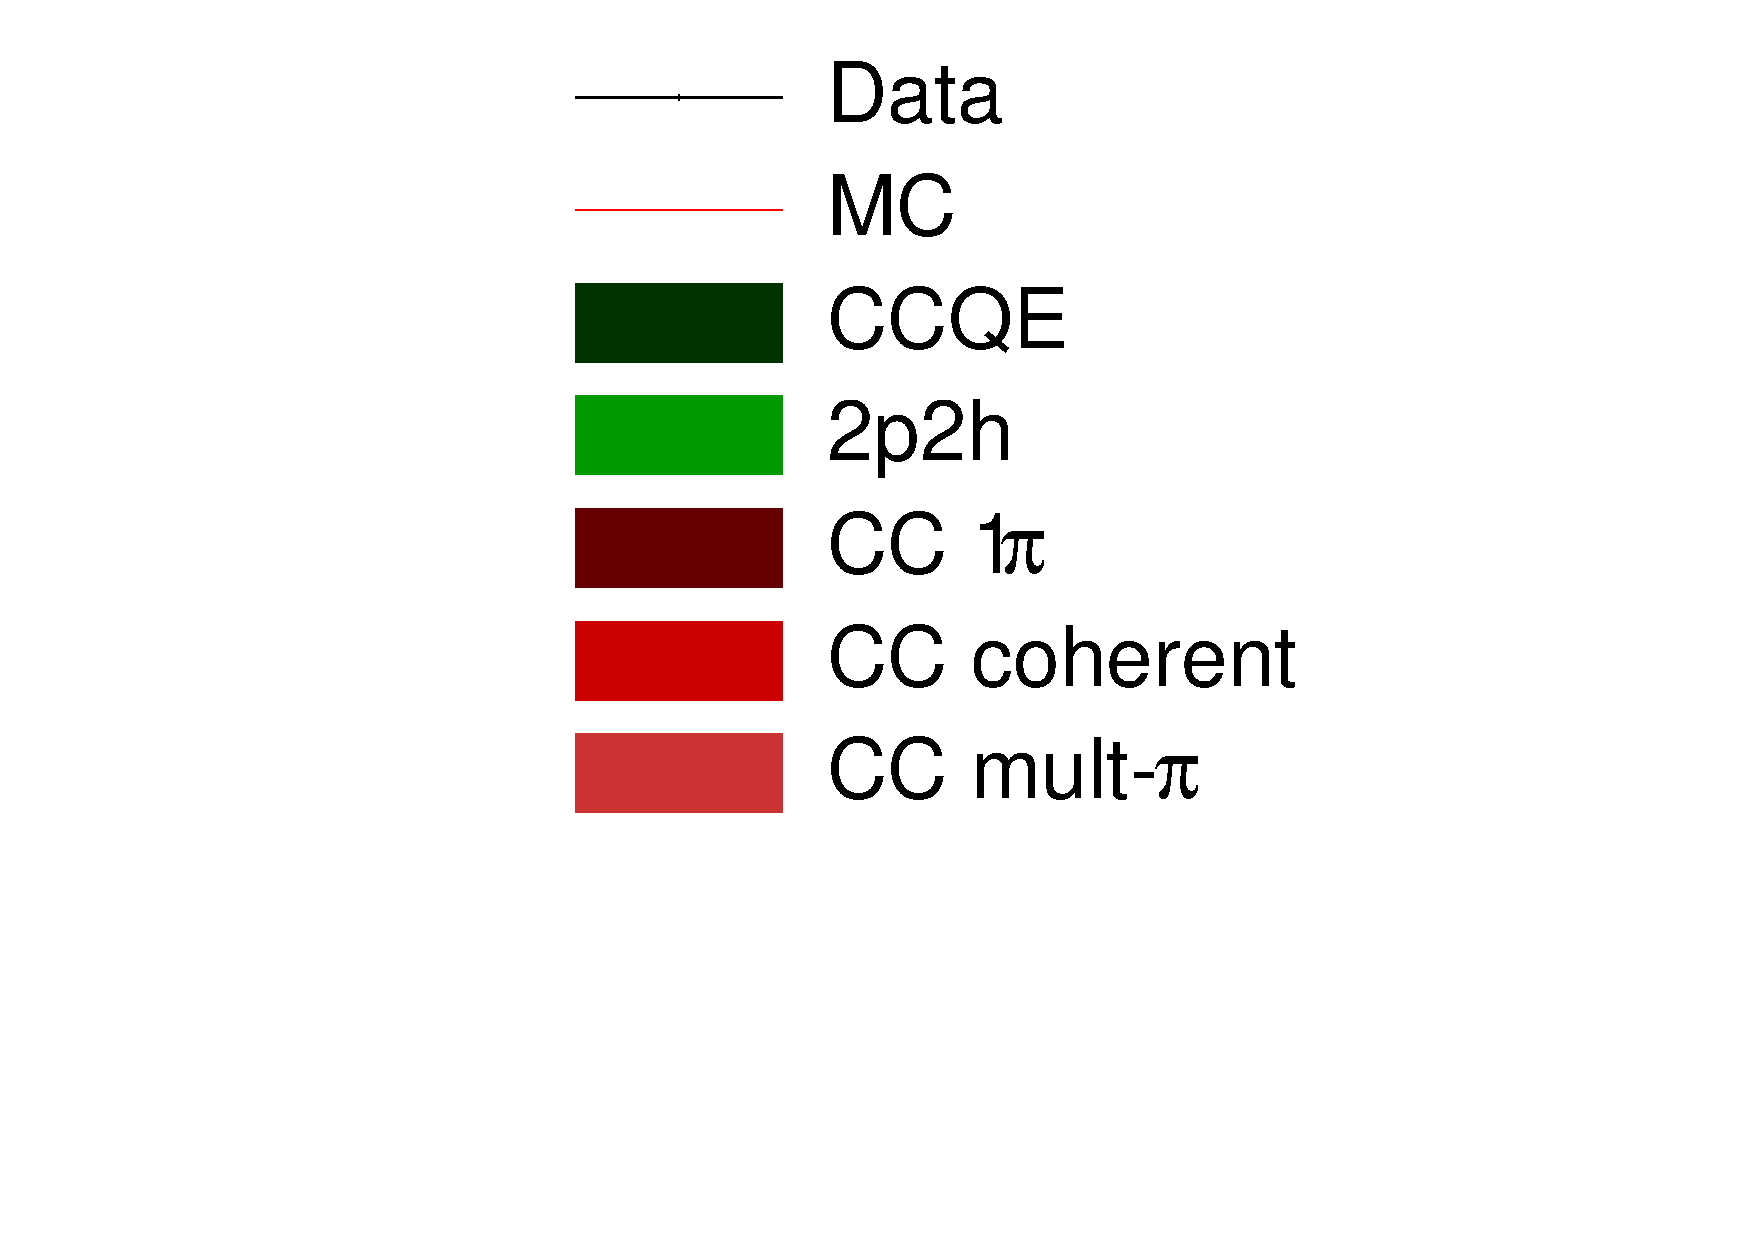
\includegraphics[width=\linewidth, trim={5mm 0mm 30mm 80mm}, clip]{figs/legend}
\end{subfigure}
\begin{subfigure}{.24\textwidth}
  \centering
  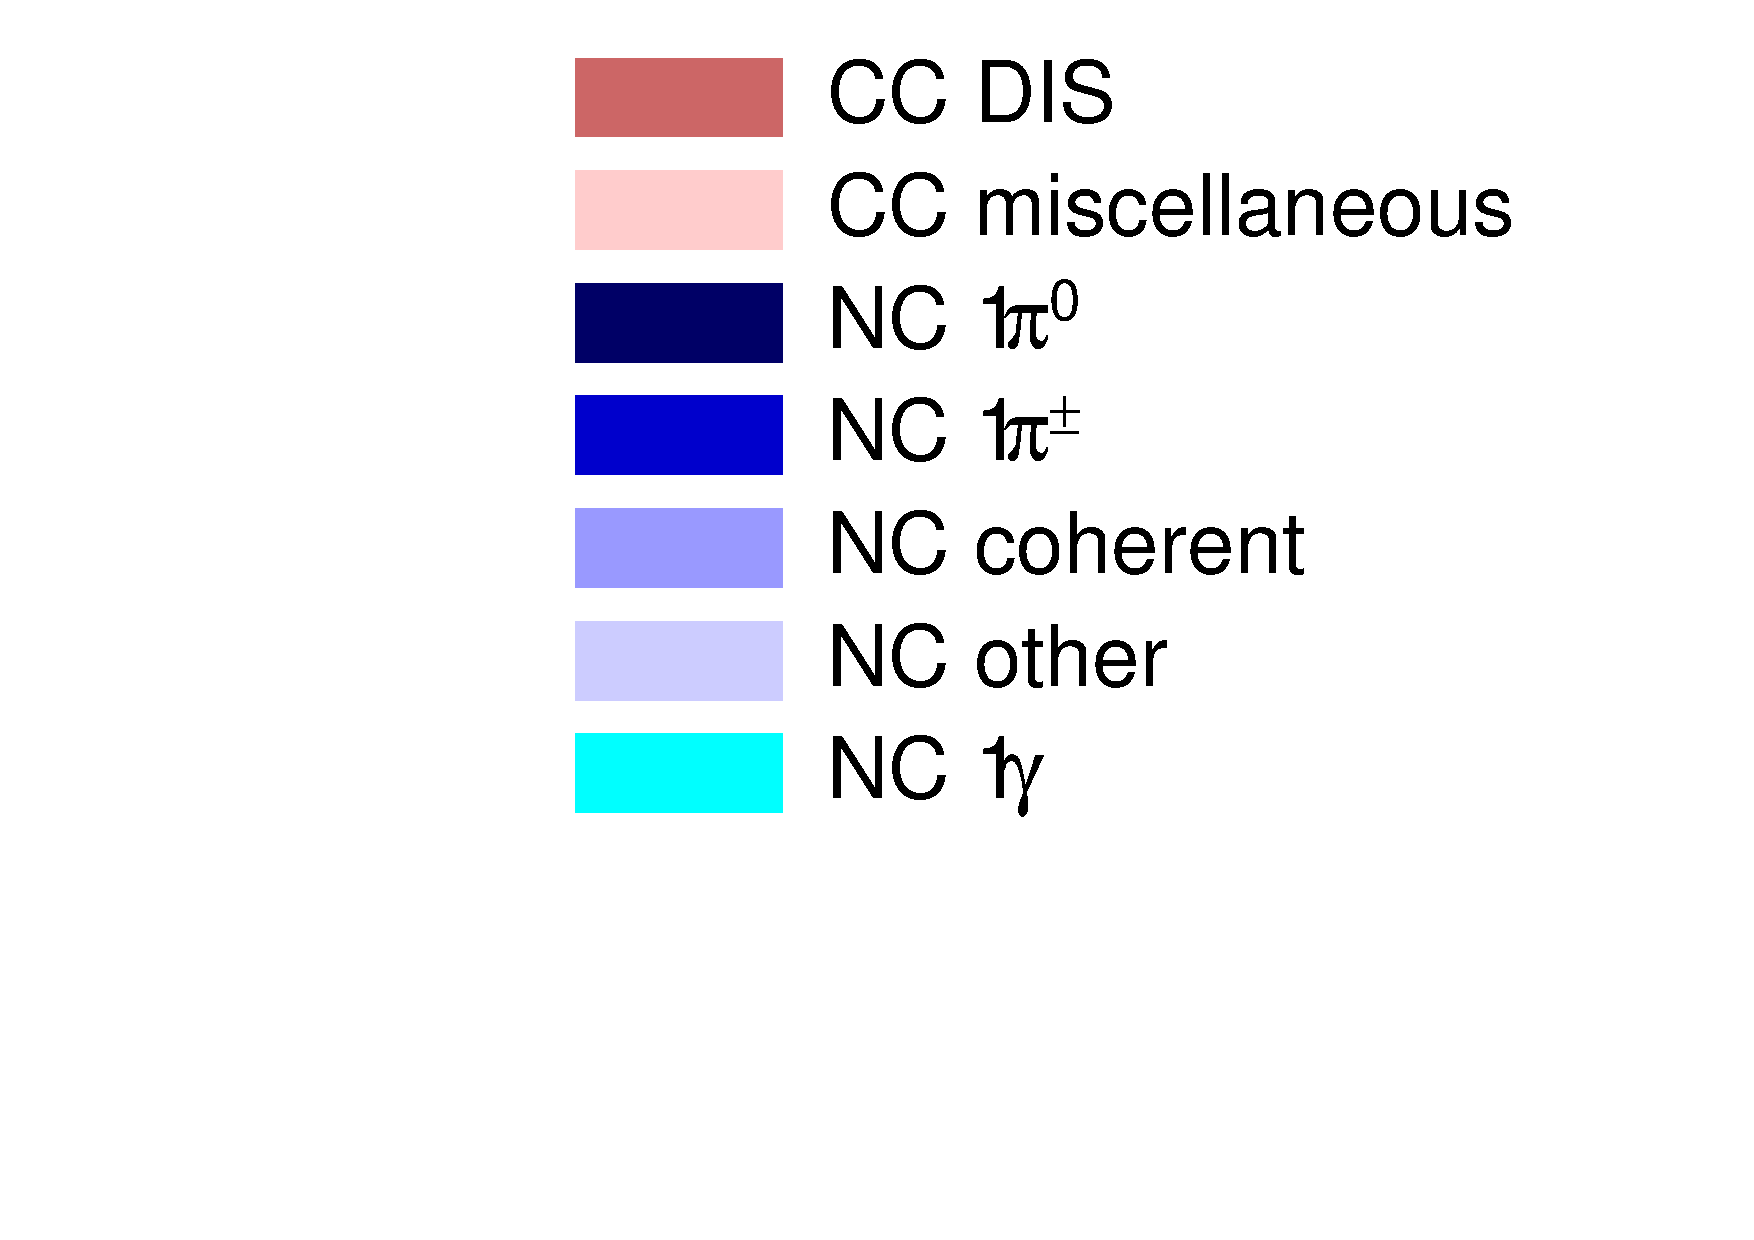
\includegraphics[width=\linewidth, trim={5mm 60mm 30mm 0mm}, clip]{figs/legend2}
\end{subfigure}
\begin{subfigure}{.24\textwidth}
  \centering
  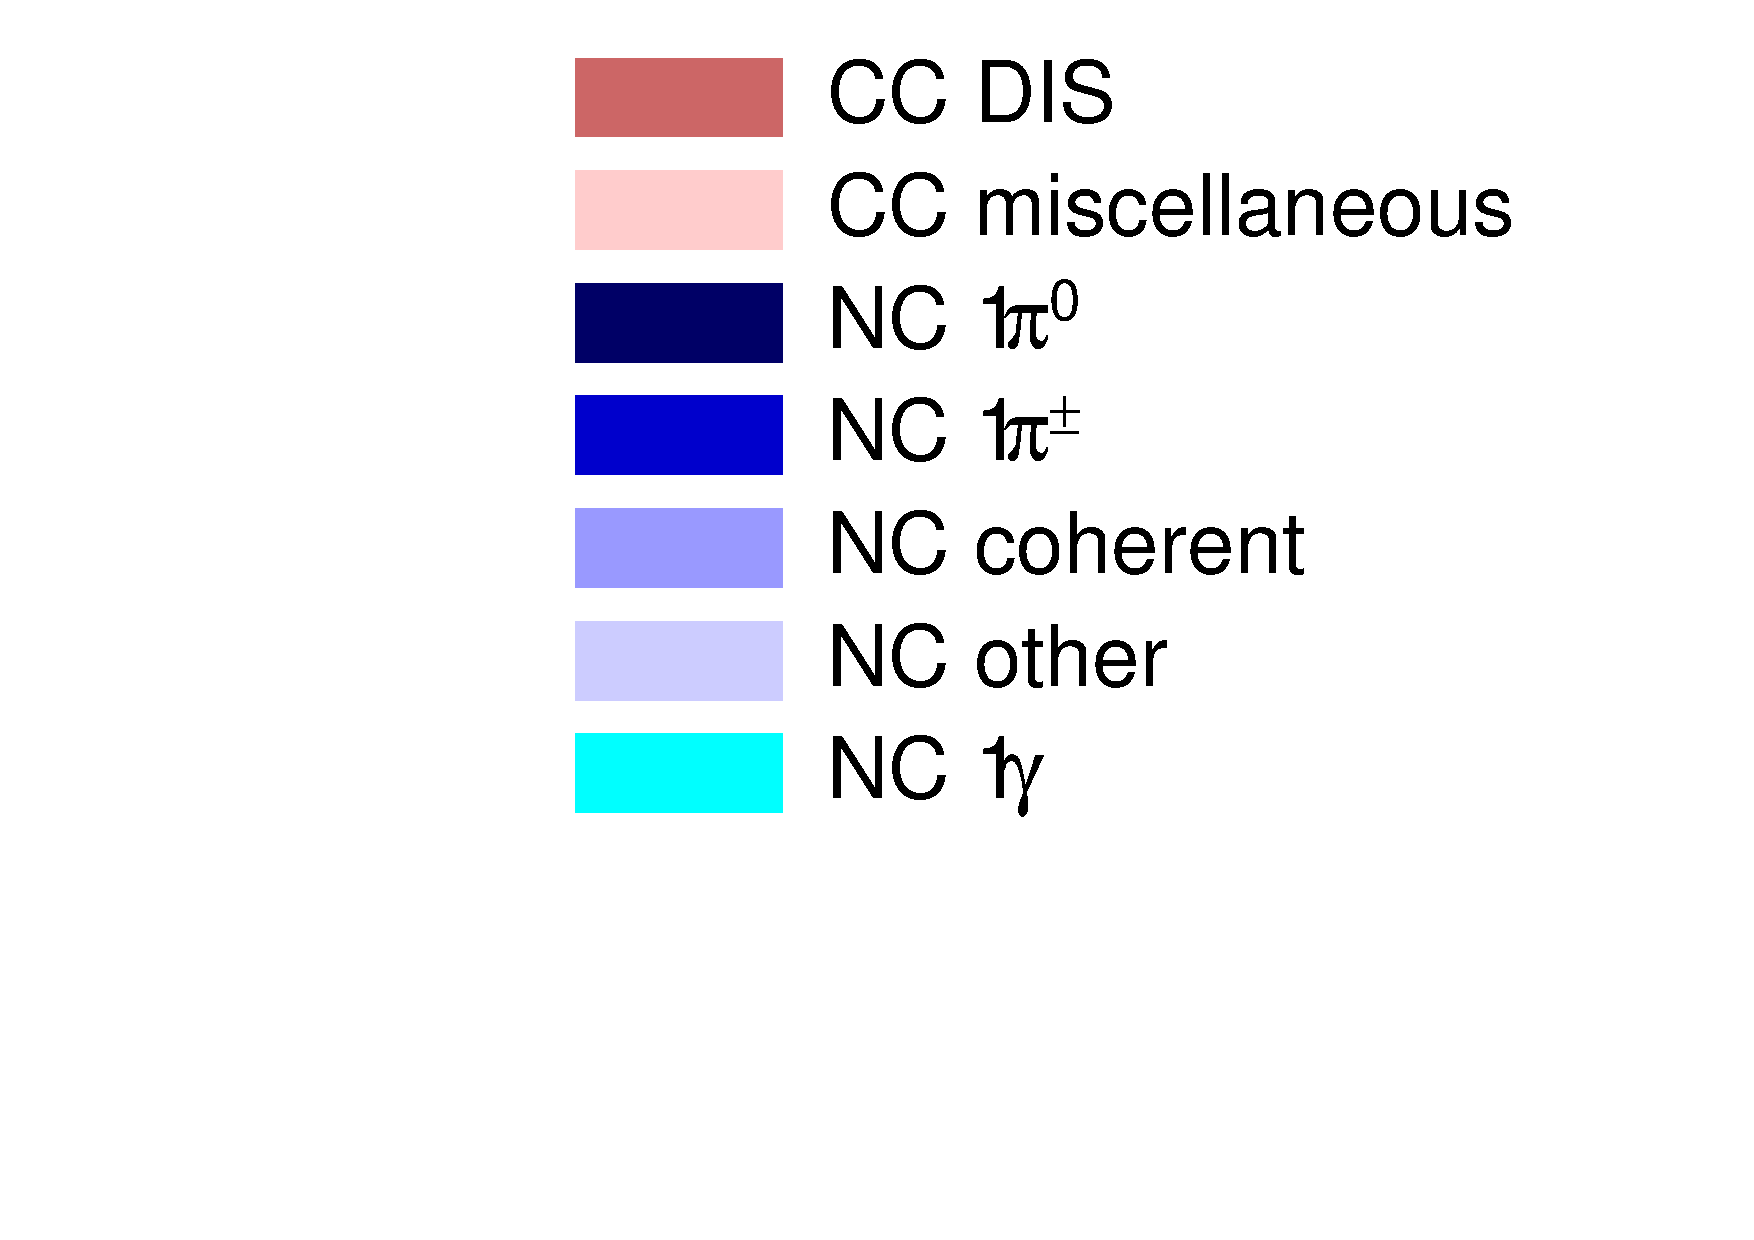
\includegraphics[width=\linewidth, trim={5mm 0mm 30mm 80mm}, clip]{figs/legend2}
\end{subfigure}

\begin{subfigure}{0.49\textwidth}
  \centering
  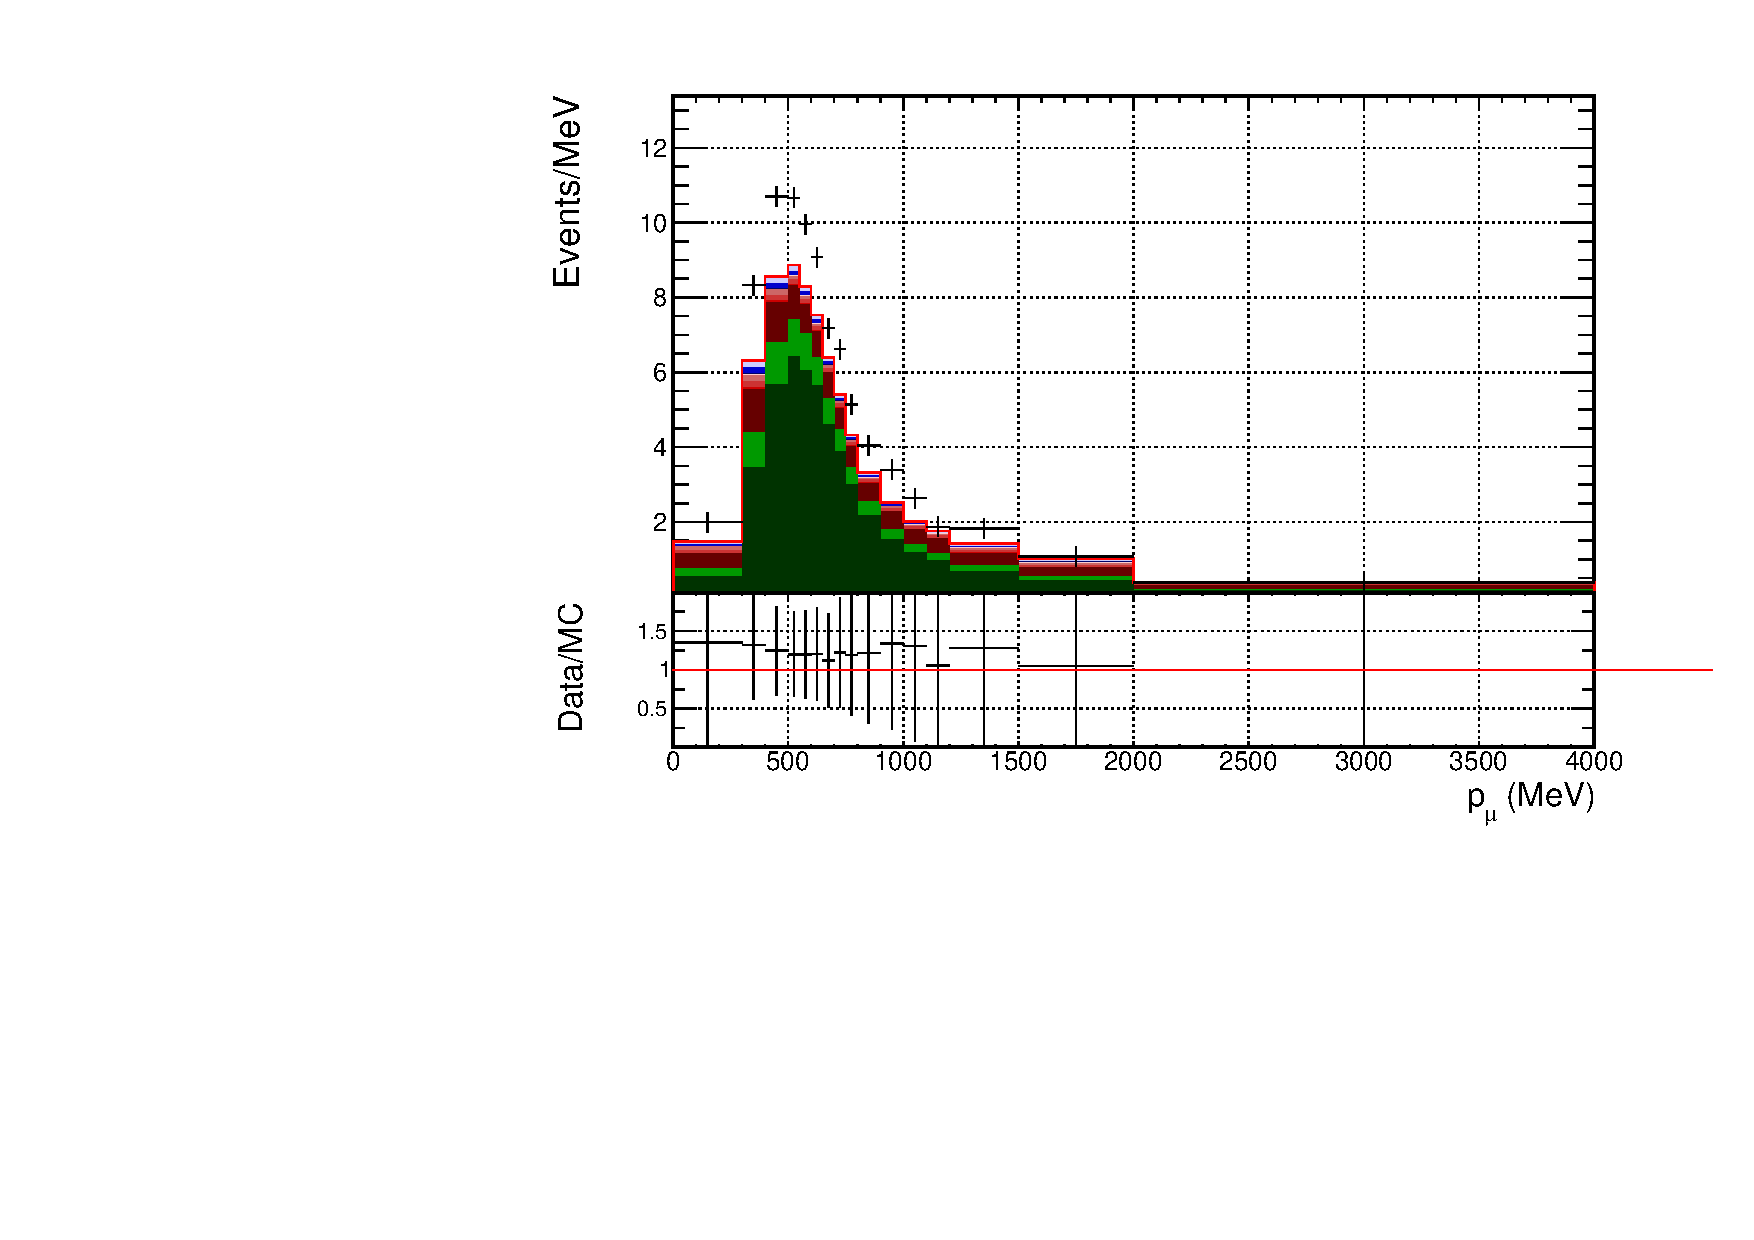
\includegraphics[width=\textwidth]{figs/FGD1_anti-numuCC_0pi_p}
  \caption{FGD1 RHC $\bar{\nu_{\mu}}$ 0$\pi$}
\end{subfigure}
\begin{subfigure}{0.49\textwidth}
  \centering
  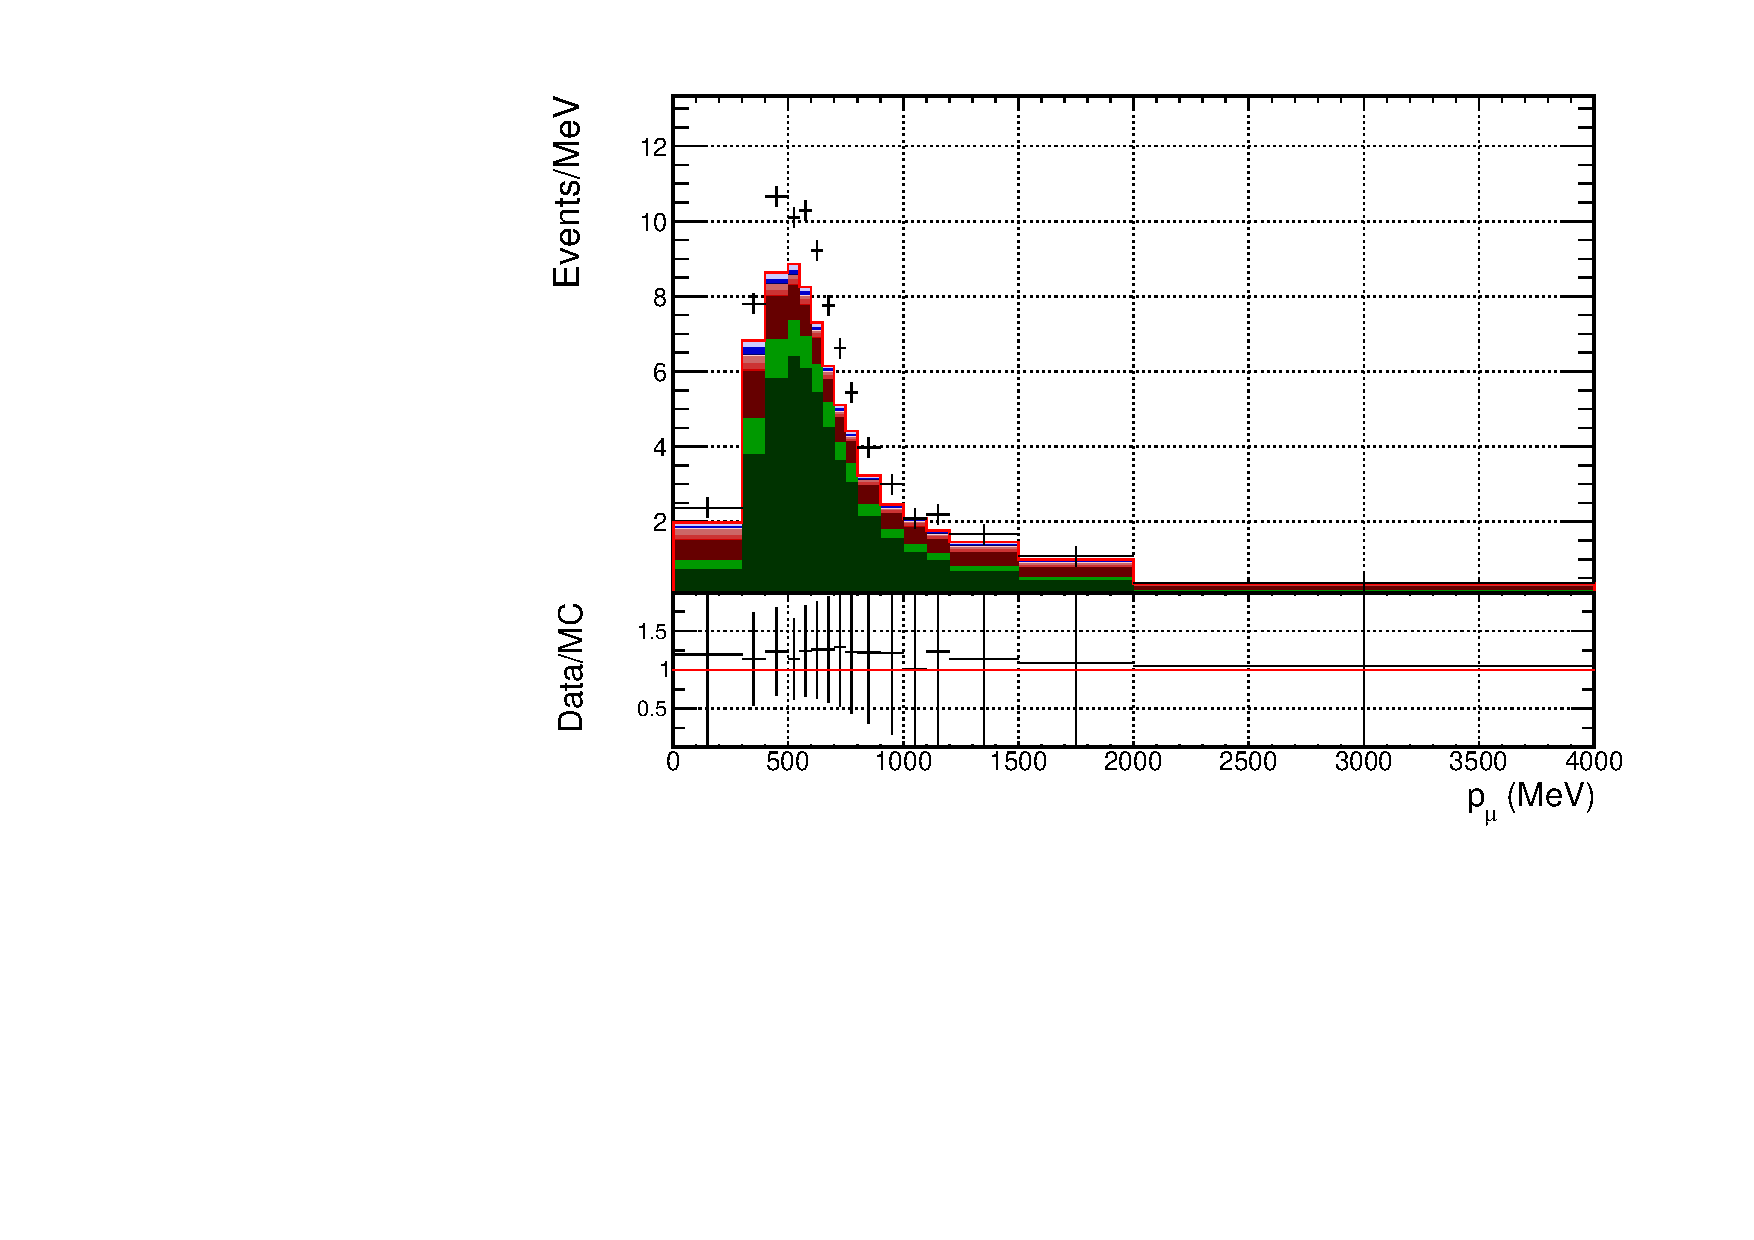
\includegraphics[width=\textwidth]{figs/FGD2_anti-numuCC_0pi_p}
  \caption{FGD2 RHC $\bar{\nu_{\mu}}$ 0$\pi$}
\end{subfigure}

\begin{subfigure}{0.49\textwidth}
  \centering
  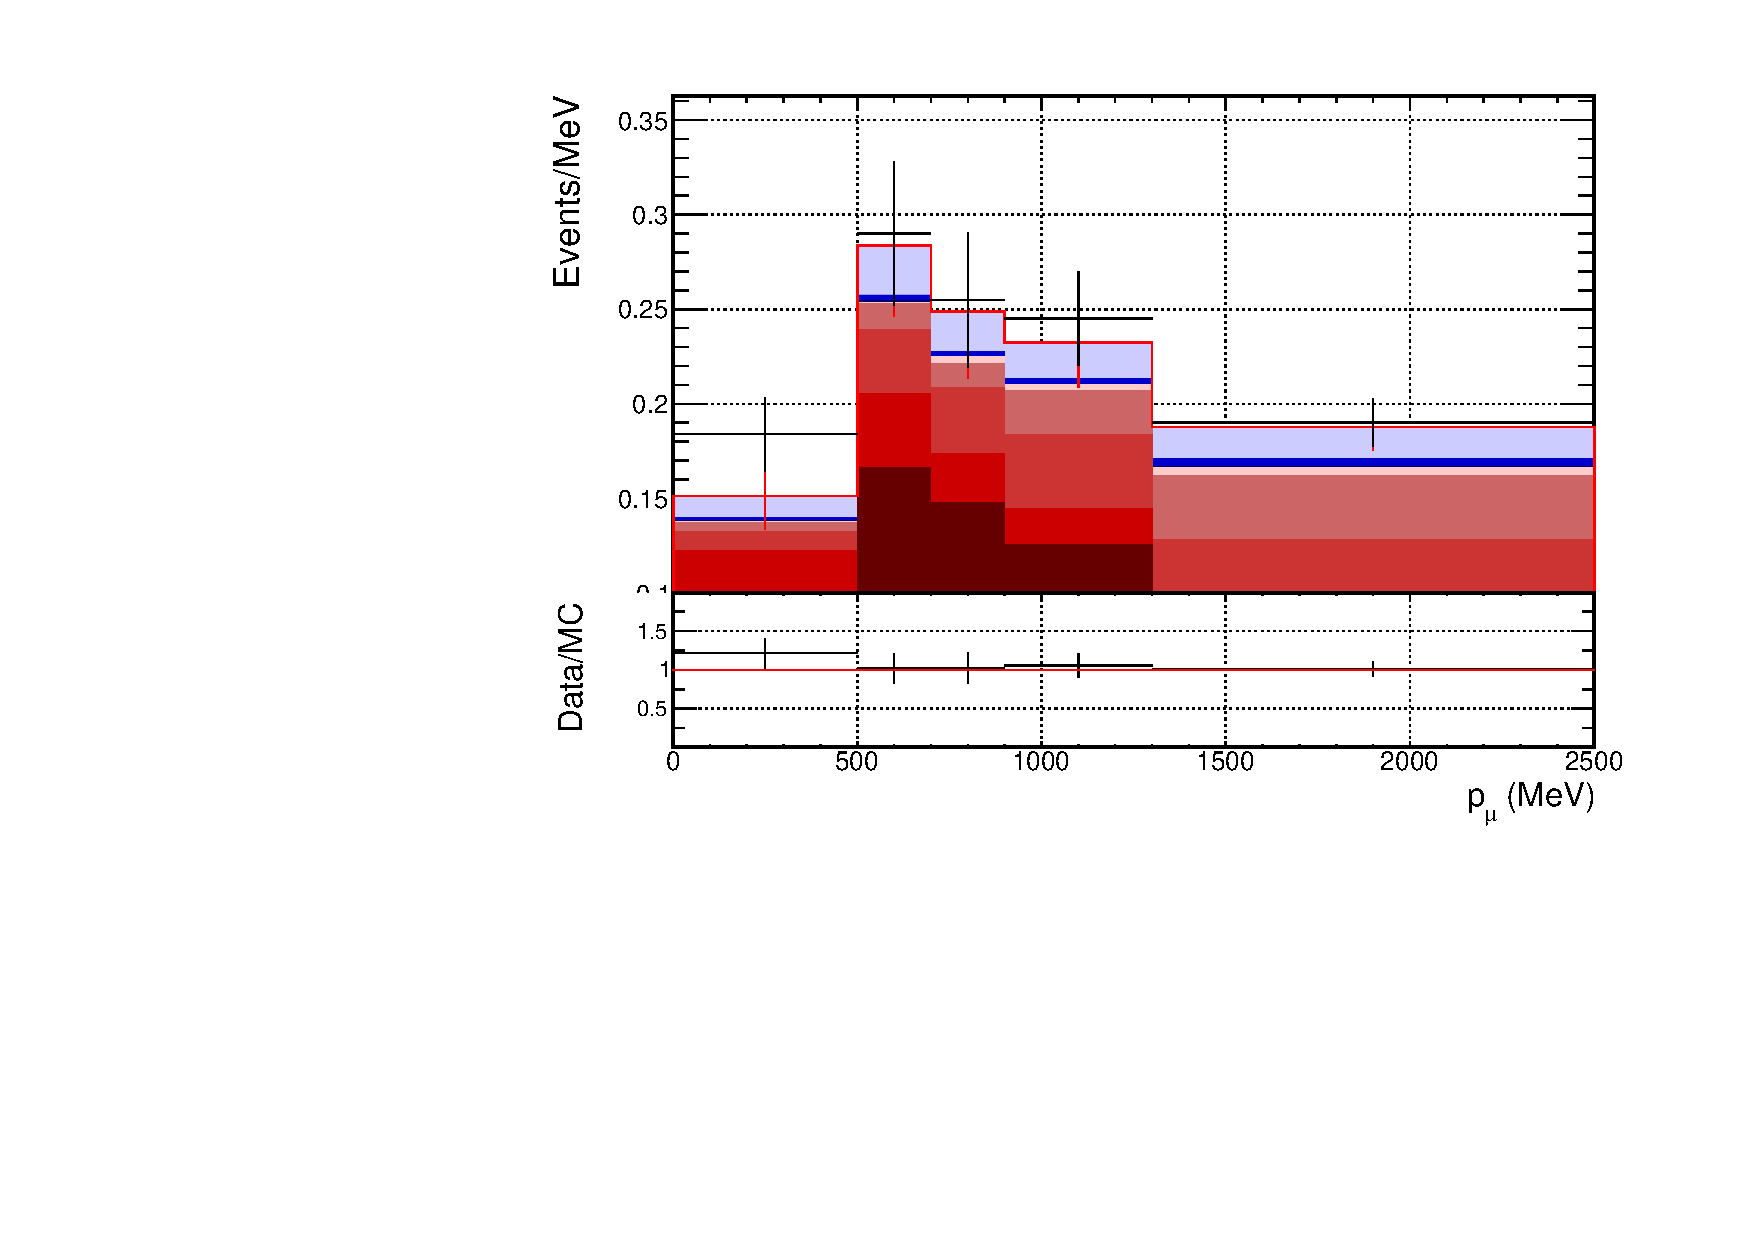
\includegraphics[width=\textwidth]{figs/FGD1_anti-numuCC_1pi_p}
  \caption{FGD1 RHC $\bar{\nu_{\mu}}$ 1$\pi$}
\end{subfigure}
\centering
\begin{subfigure}{0.49\textwidth}
  \centering
  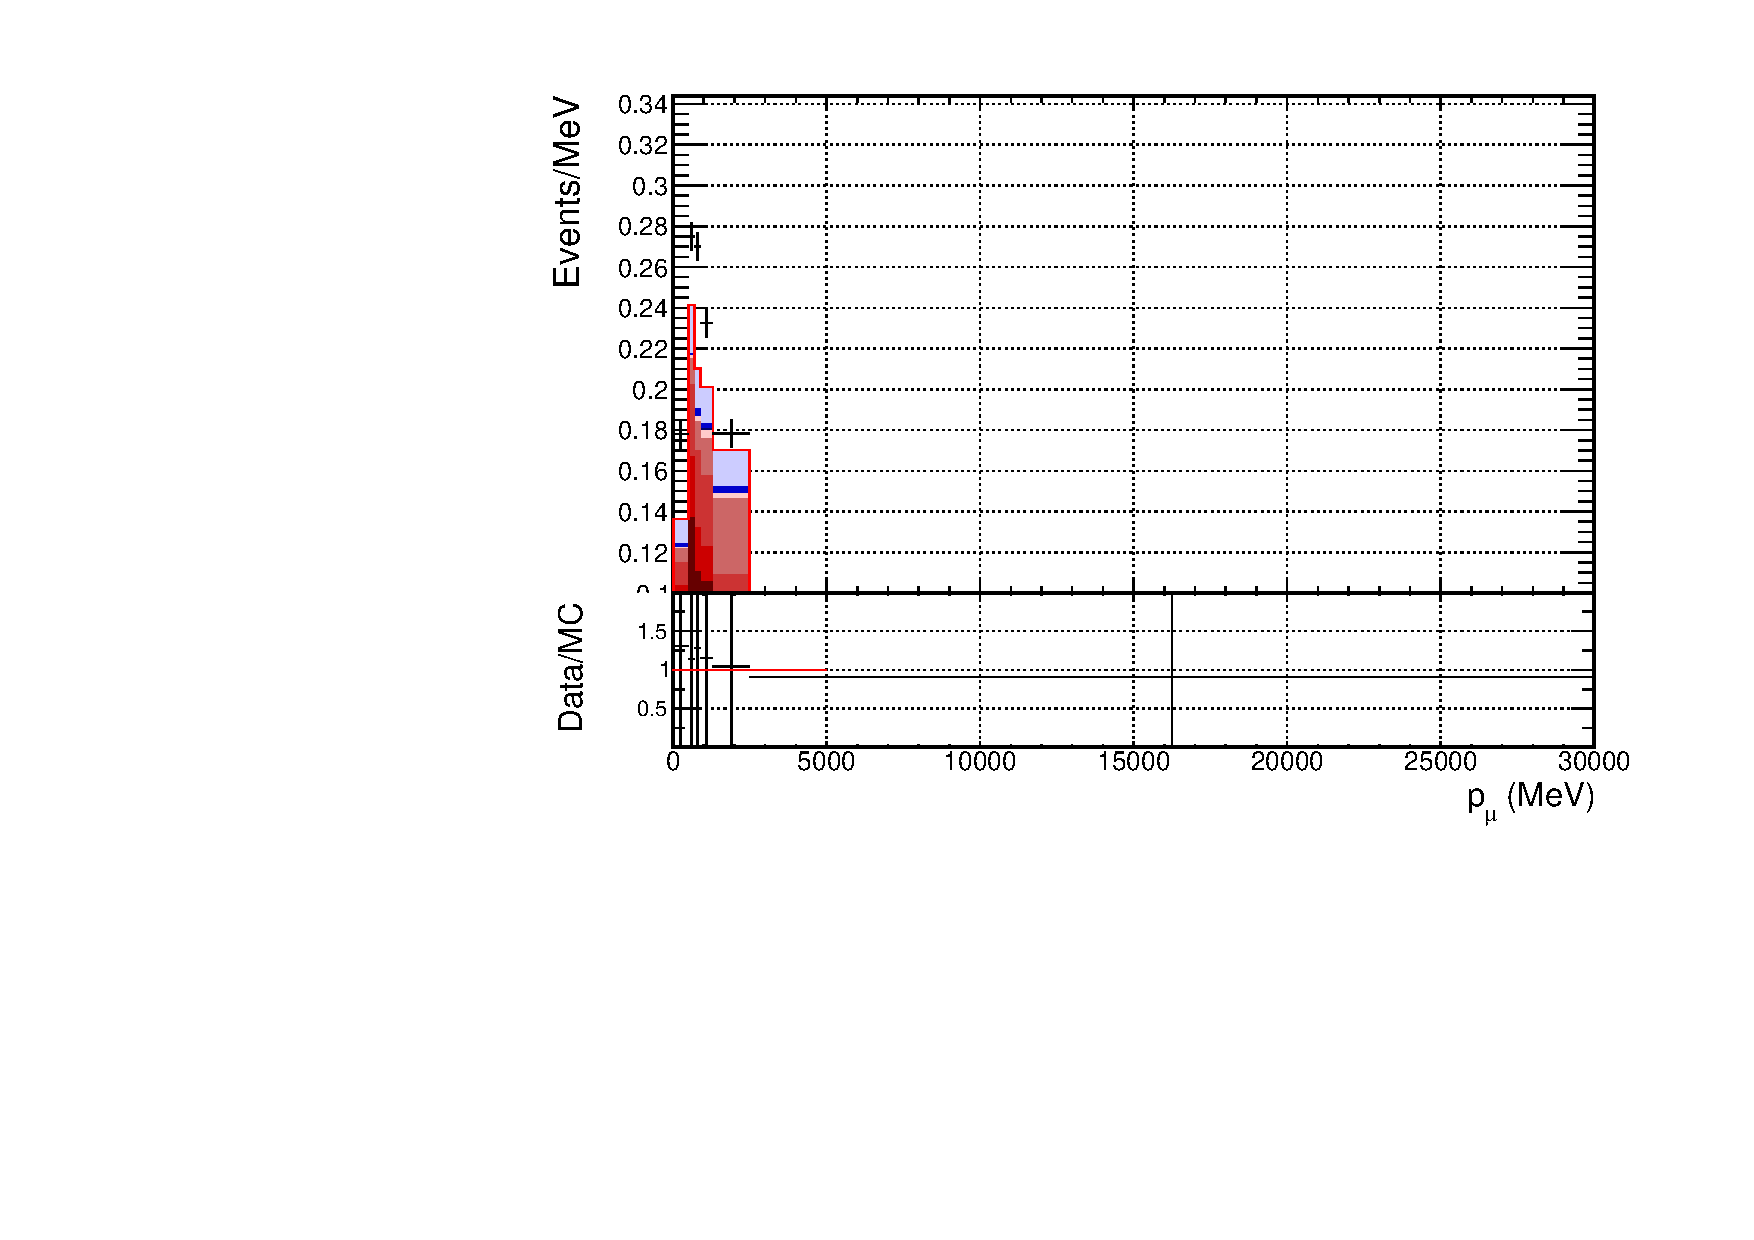
\includegraphics[width=\textwidth]{figs/FGD2_anti-numuCC_1pi_p}
  \caption{FGD2 RHC $\bar{\nu_{\mu}}$ 1$\pi$}
\end{subfigure}

\begin{subfigure}{0.49\textwidth}
  \centering
  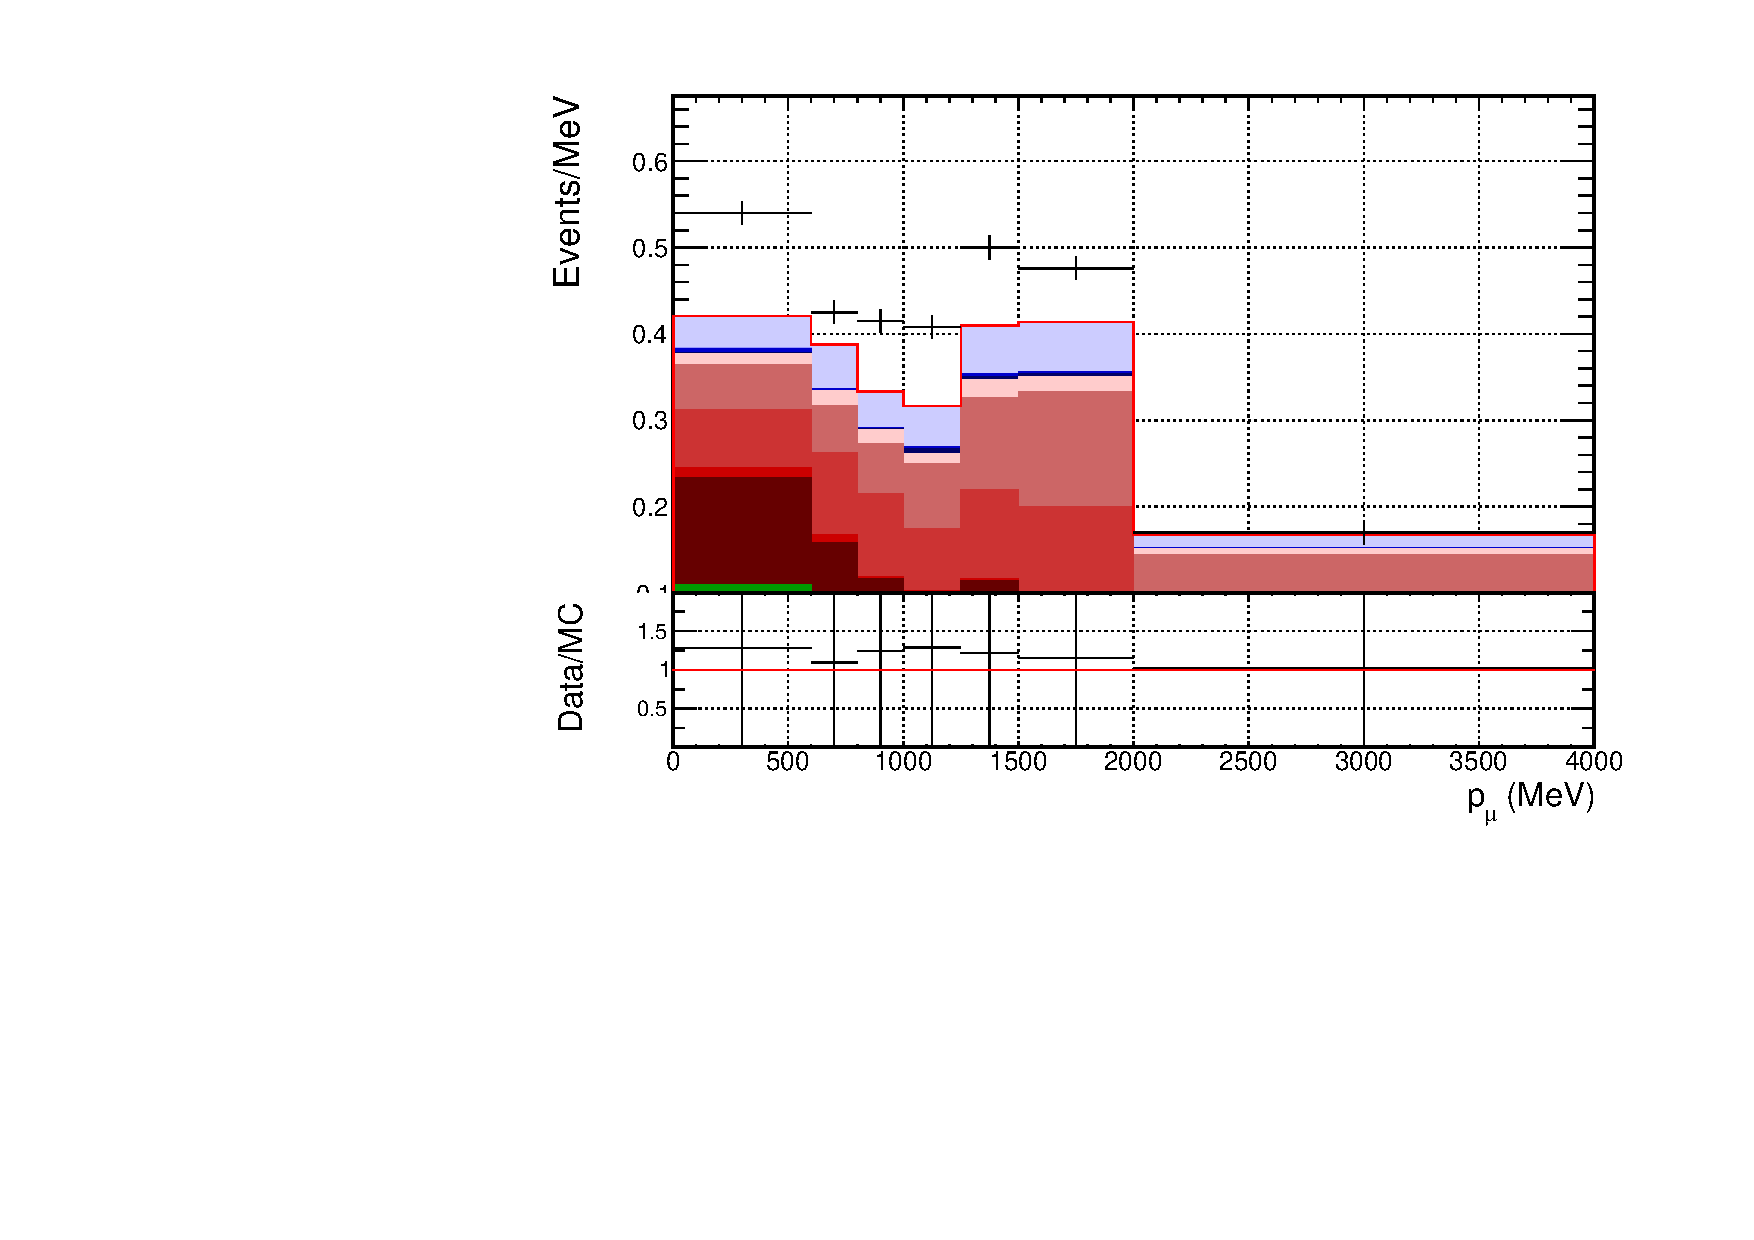
\includegraphics[width=\textwidth]{figs/FGD1_anti-numuCC_other_p}
  \caption{FGD1 RHC $\bar{\nu_{\mu}}$ Other}
\end{subfigure}
\begin{subfigure}{0.49\textwidth}
  \centering
  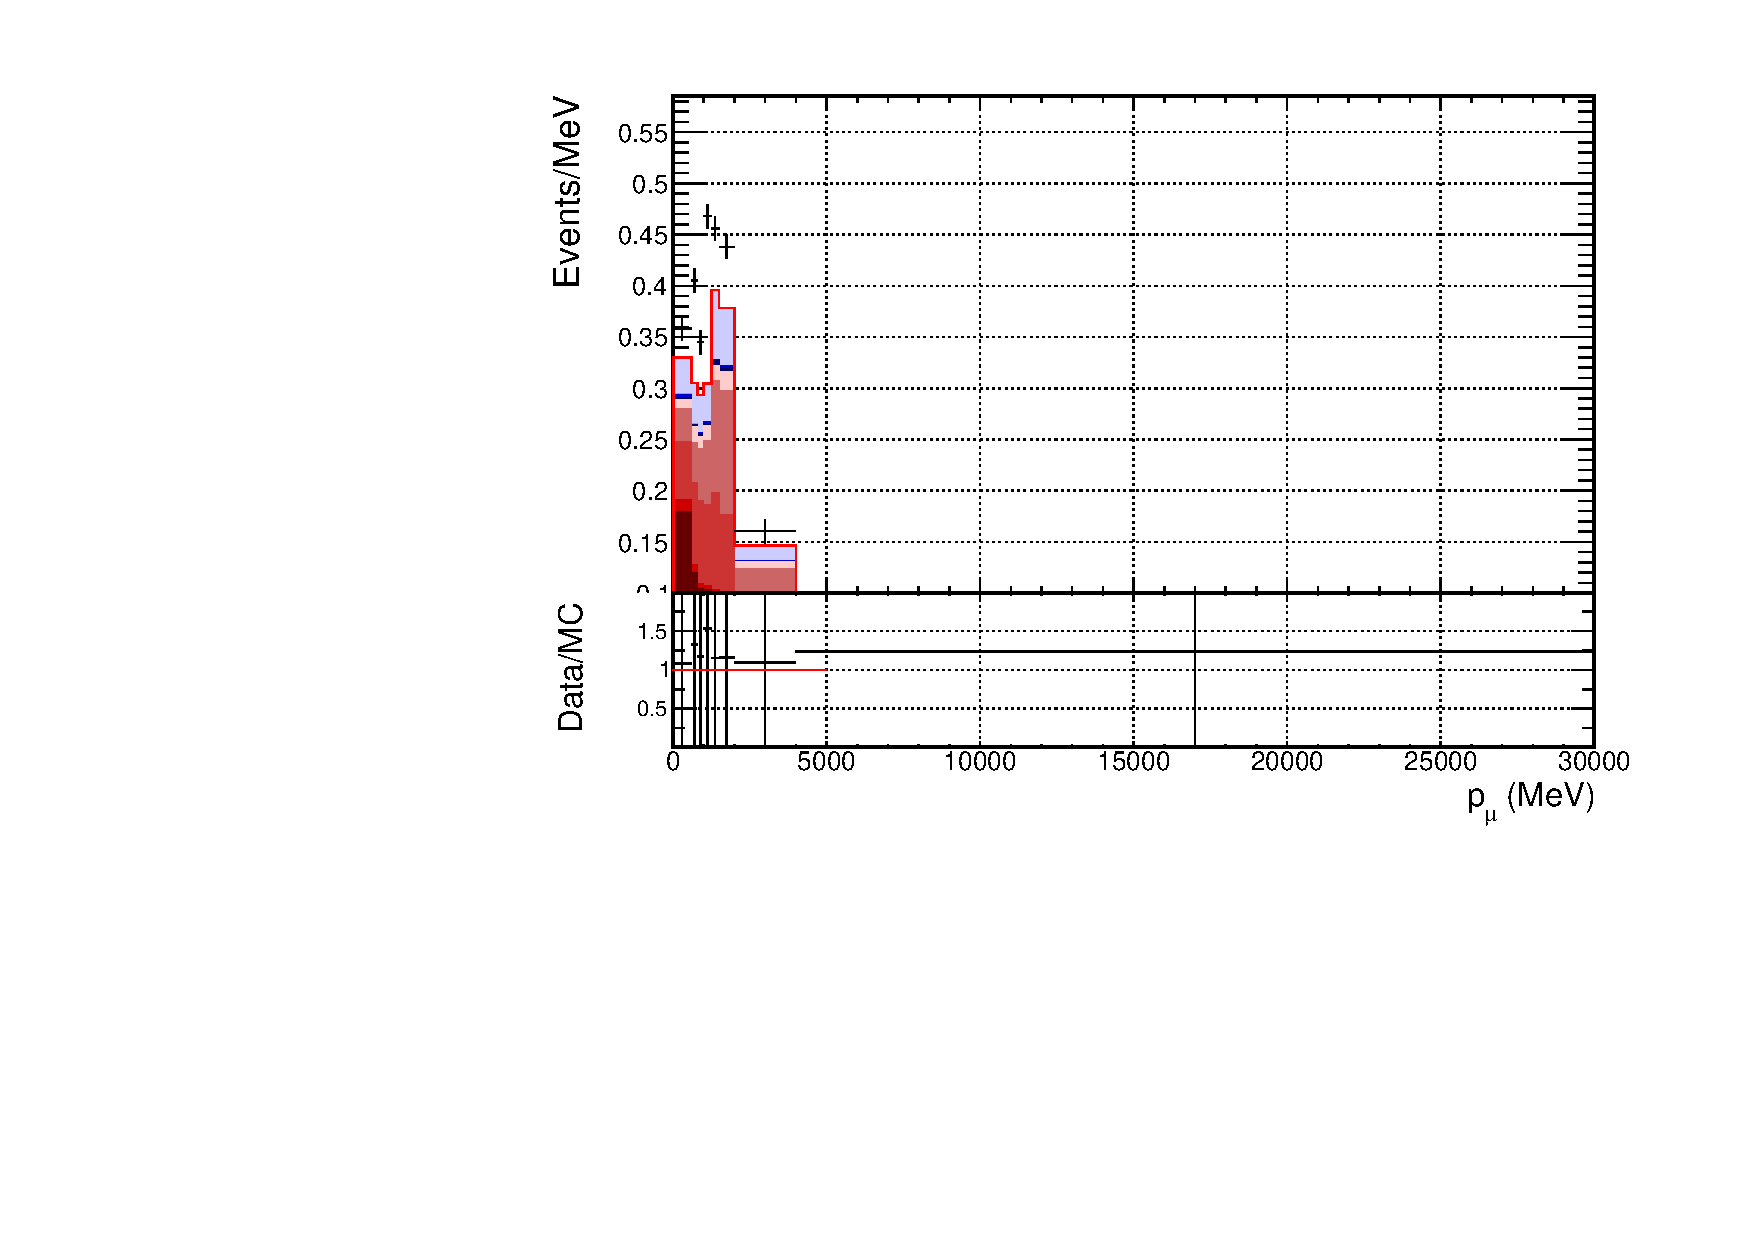
\includegraphics[width=\textwidth]{figs/FGD2_anti-numuCC_other_p}
  \caption{FGD2 RHC $\bar{\nu_{\mu}}$ Other}
\end{subfigure}
\caption{$p_{\mu}$ projections of data and nominal MC broken down by interaction mode for RHC \numub selections.}
\label{fig:pstack_rhc_numub}
\end{figure}

\begin{figure}[!h]
\centering
\begin{subfigure}{.24\textwidth}
  \centering
  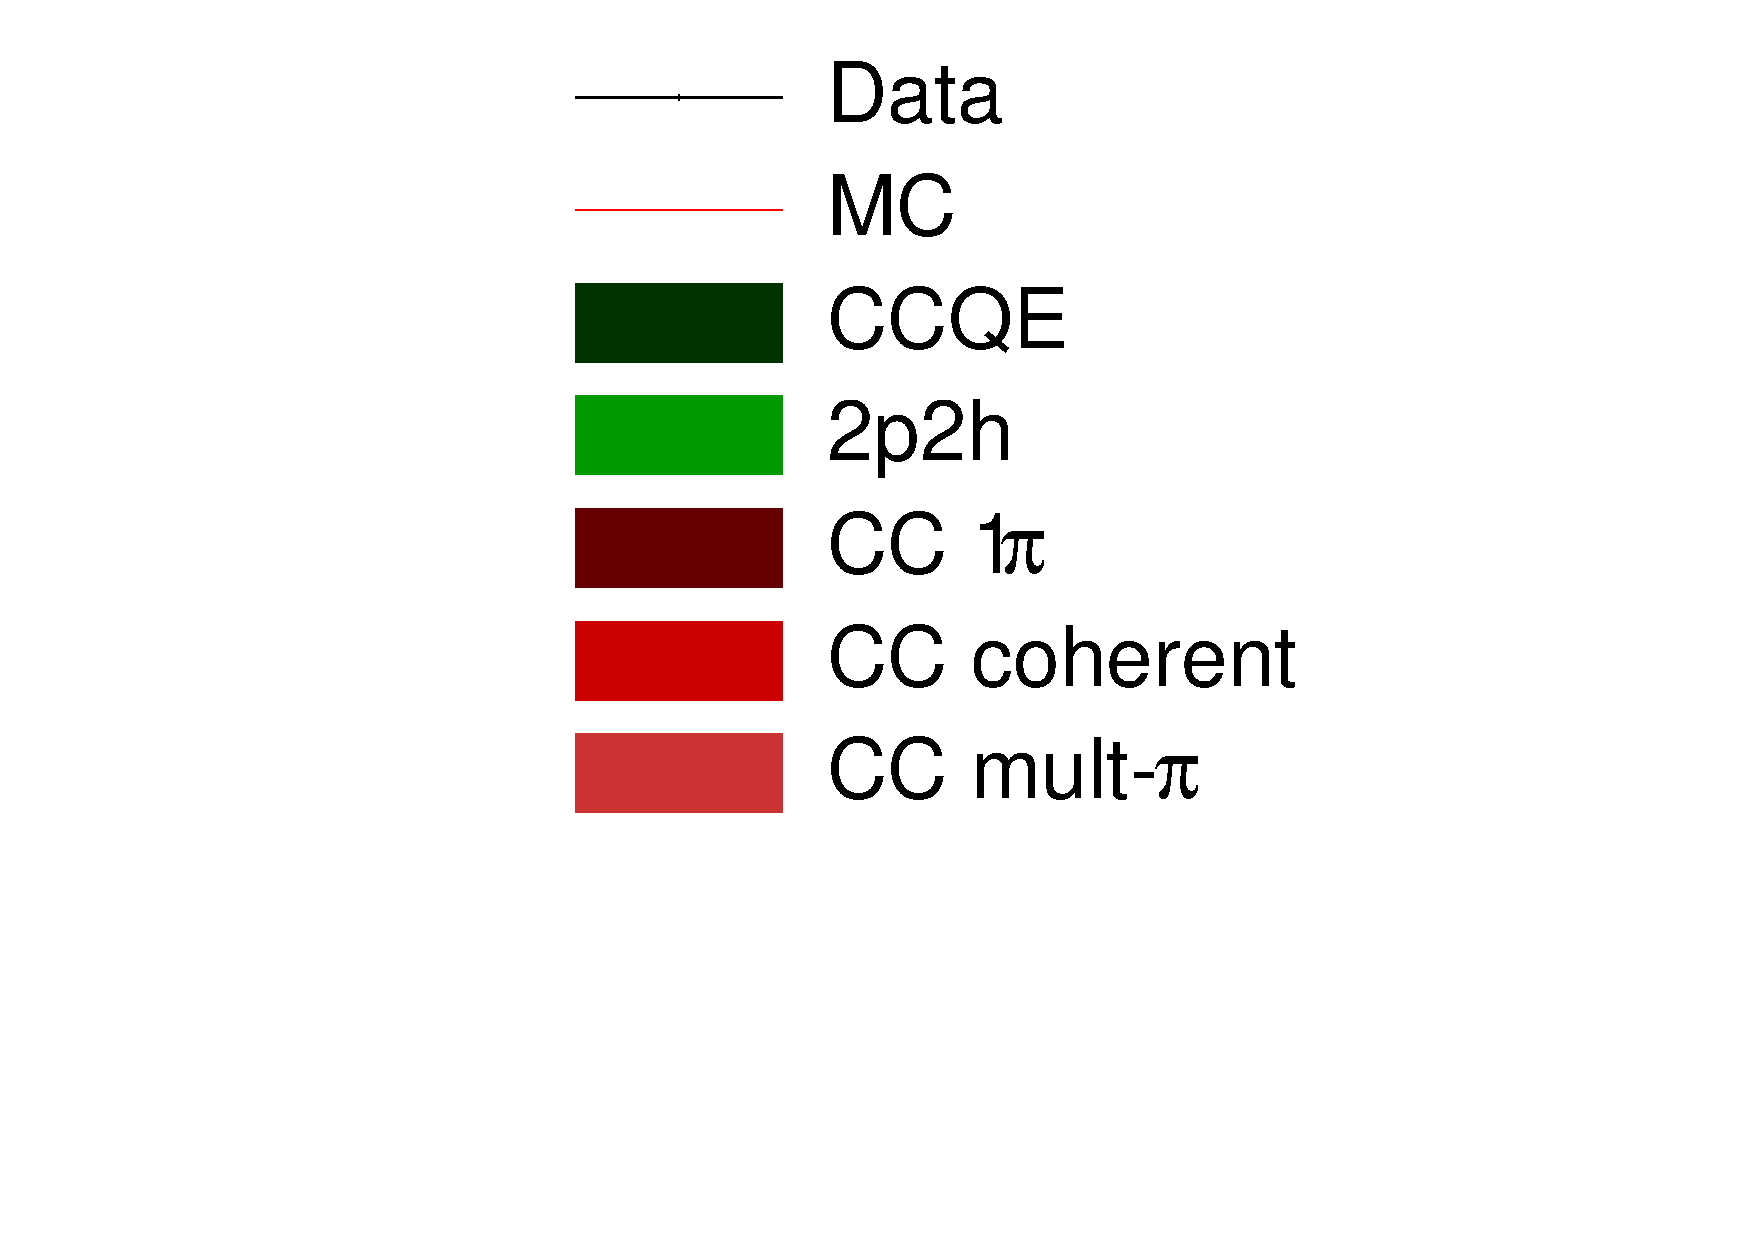
\includegraphics[width=\linewidth, trim={5mm 60mm 30mm 0mm}, clip]{figs/legend}
\end{subfigure}
\begin{subfigure}{.24\textwidth}
  \centering
  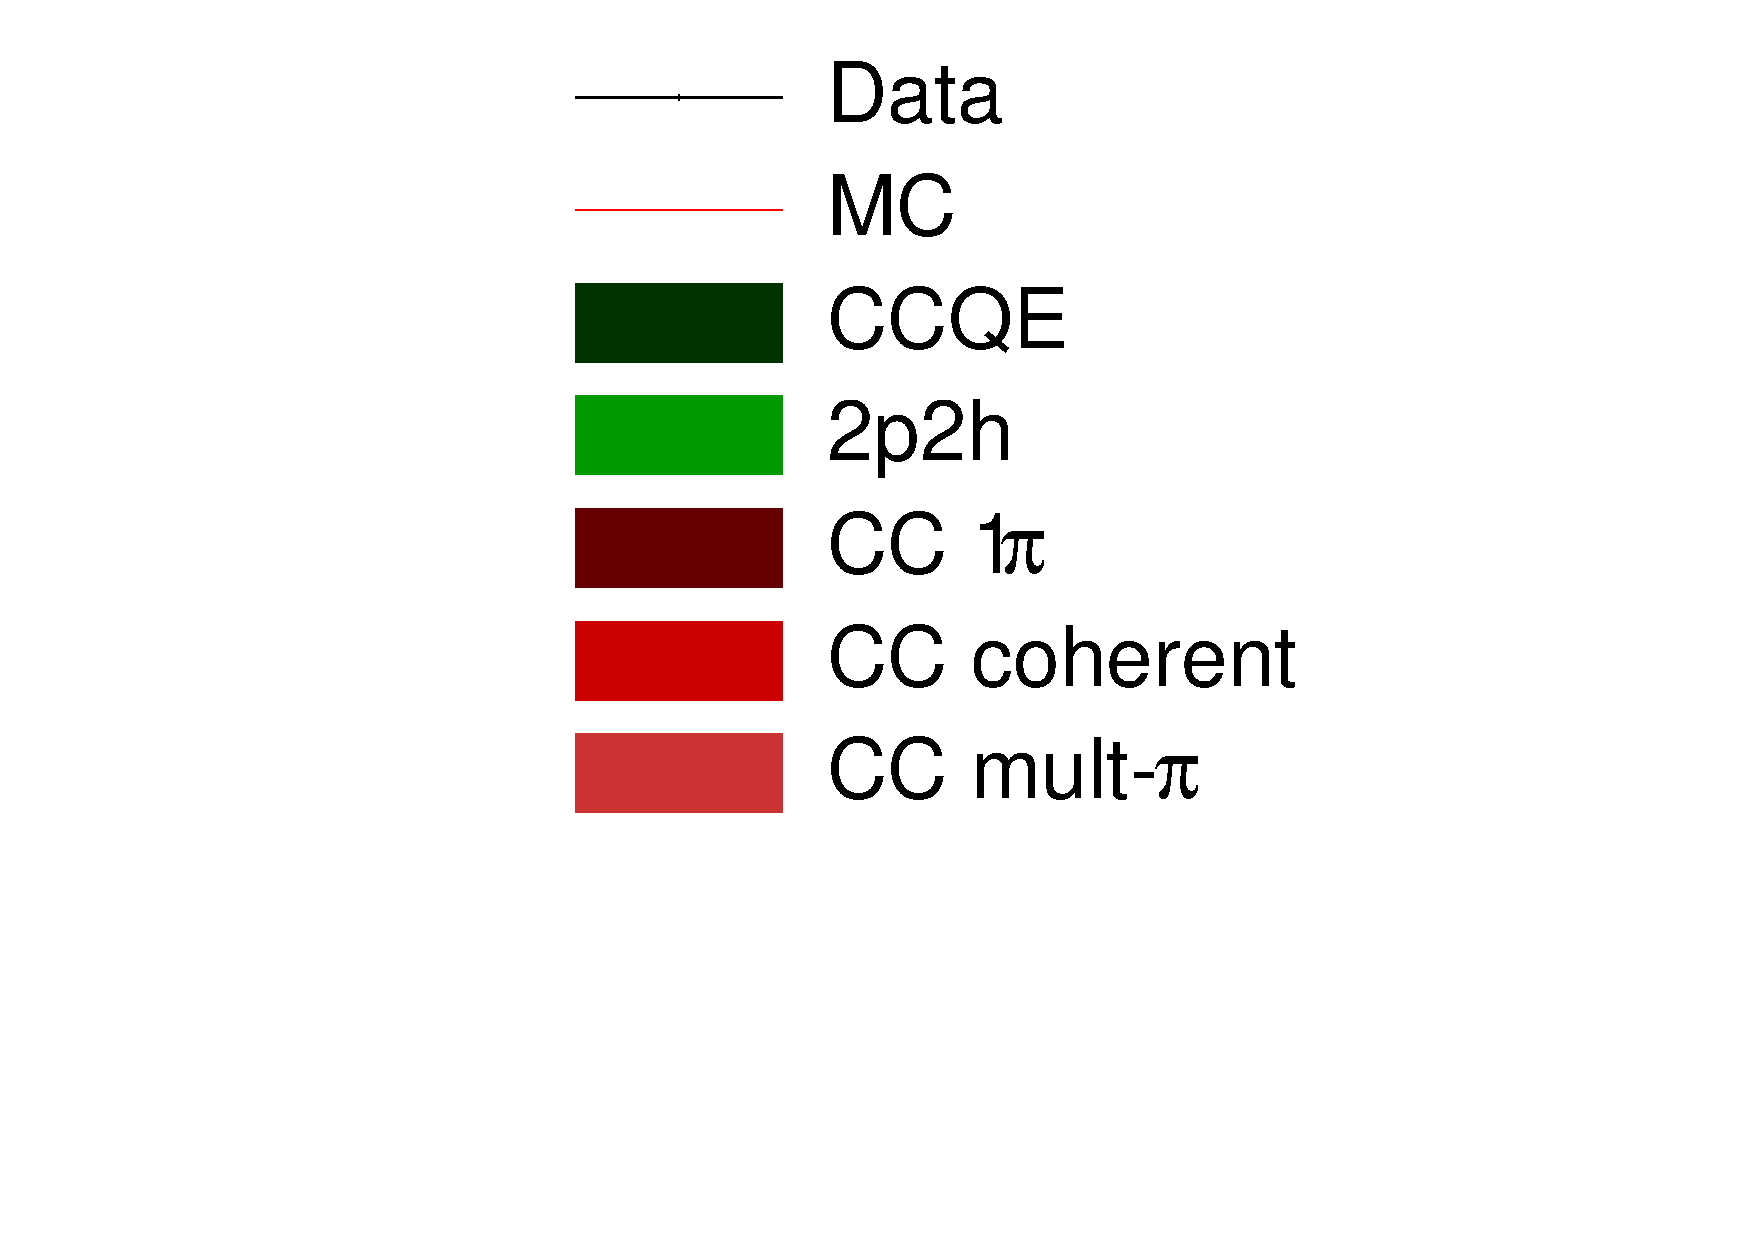
\includegraphics[width=\linewidth, trim={5mm 0mm 30mm 80mm}, clip]{figs/legend}
\end{subfigure}
\begin{subfigure}{.24\textwidth}
  \centering
  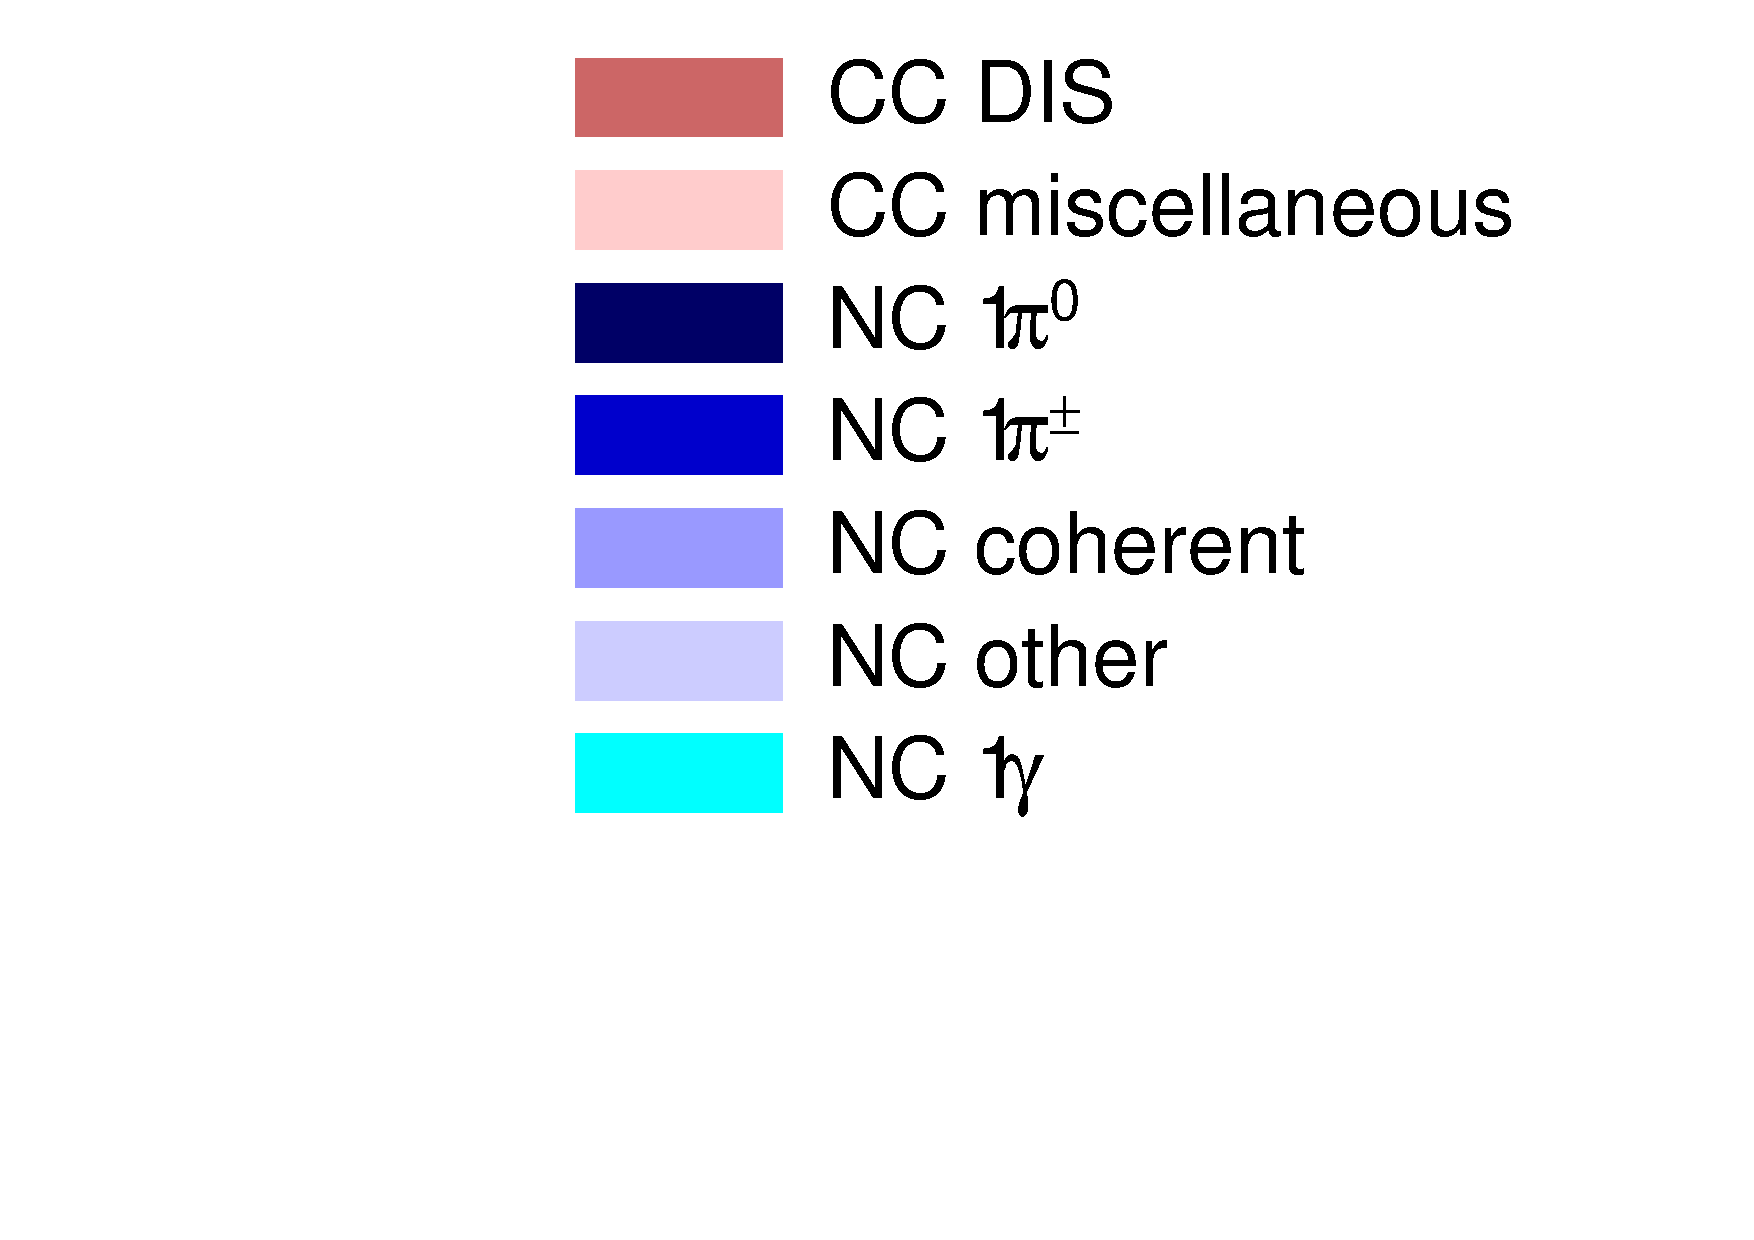
\includegraphics[width=\linewidth, trim={5mm 60mm 30mm 0mm}, clip]{figs/legend2}
\end{subfigure}
\begin{subfigure}{.24\textwidth}
  \centering
  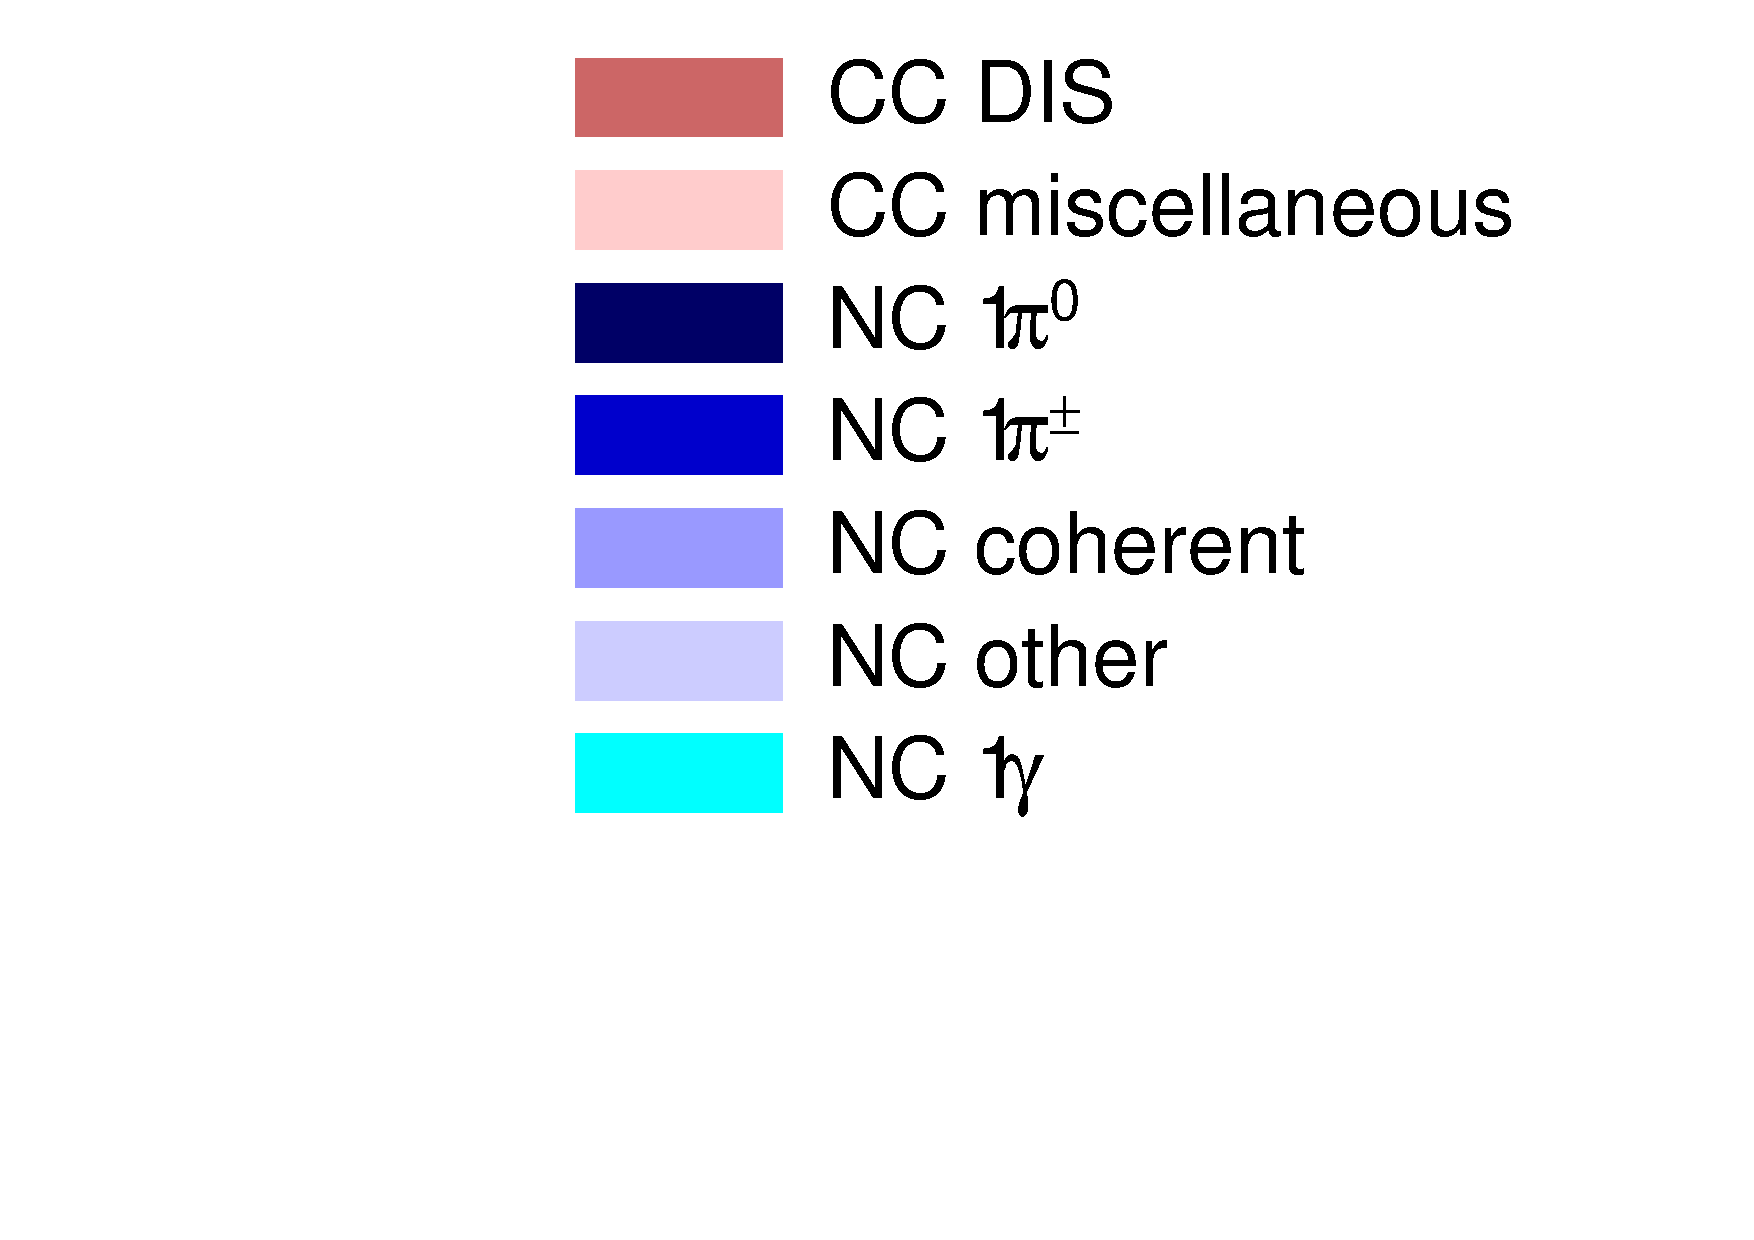
\includegraphics[width=\linewidth, trim={5mm 0mm 30mm 80mm}, clip]{figs/legend2}
\end{subfigure}

\begin{subfigure}{0.49\textwidth}
  \centering
  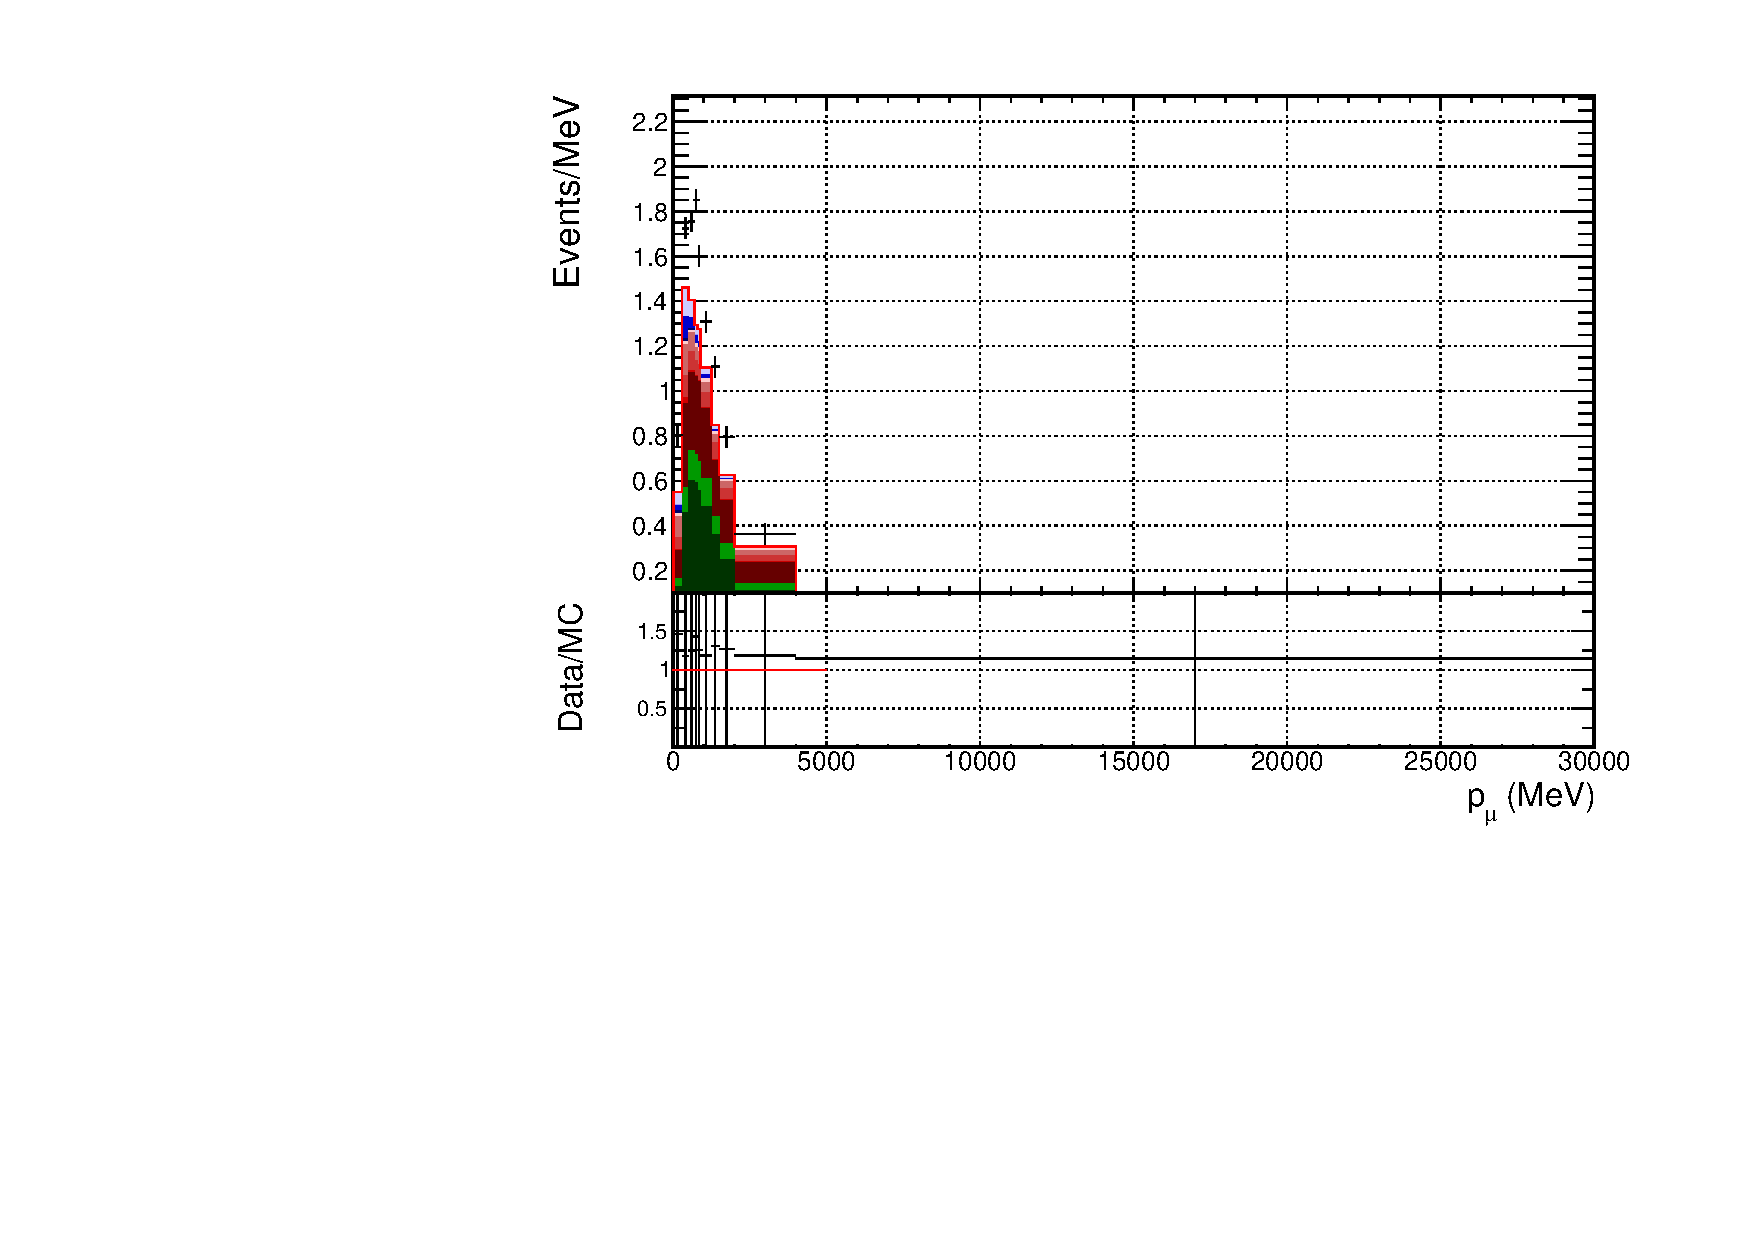
\includegraphics[width=\textwidth]{figs/FGD1_NuMuBkg_CC0pi_in_AntiNu_Mode_p}
  \caption{FGD1 RHC $\nu_{\mu}$ 0$\pi$}
\end{subfigure}
\begin{subfigure}{0.49\textwidth}
  \centering
  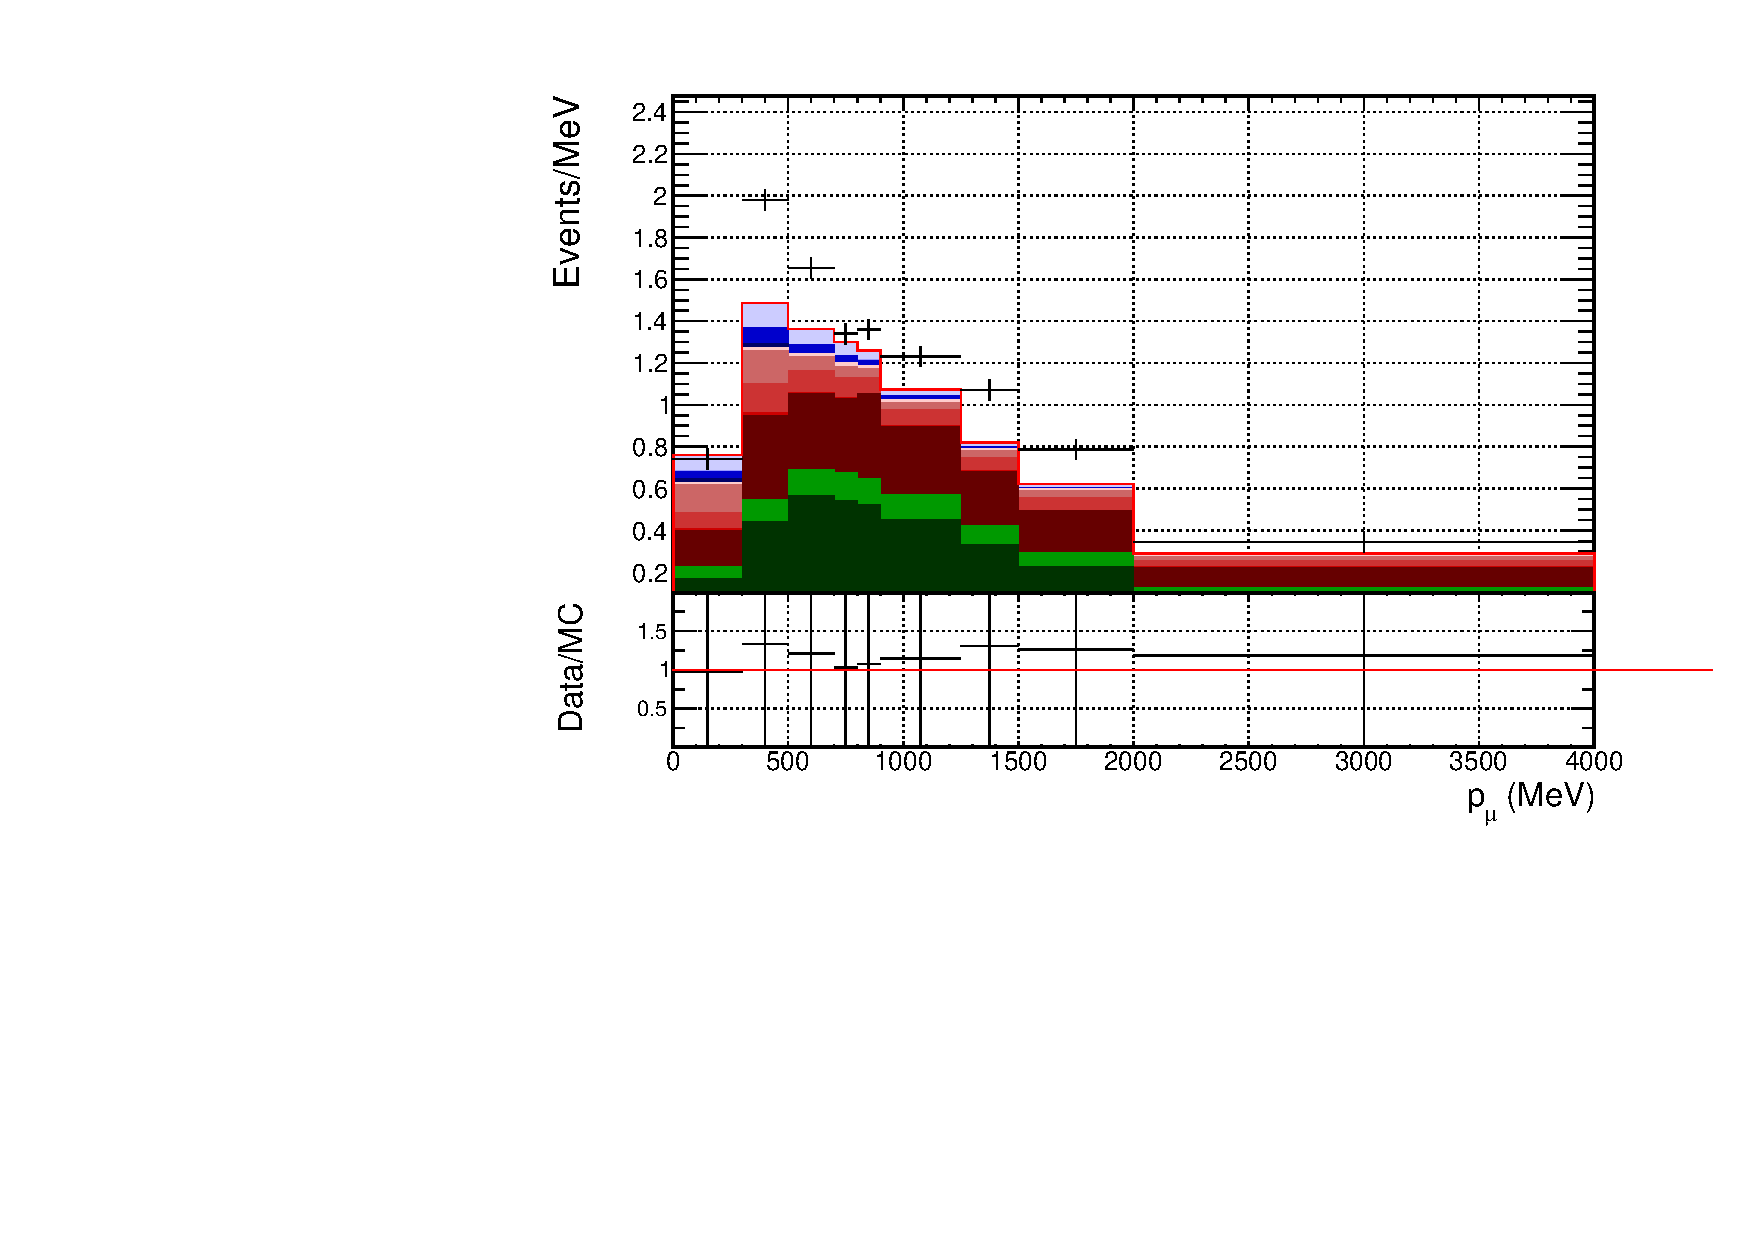
\includegraphics[width=\textwidth]{figs/FGD2_NuMuBkg_CC0pi_in_AntiNu_Mode_p}
  \caption{FGD2 RHC $\nu_{\mu}$ 0$\pi$}
\end{subfigure}

\begin{subfigure}{0.49\textwidth}
  \centering
  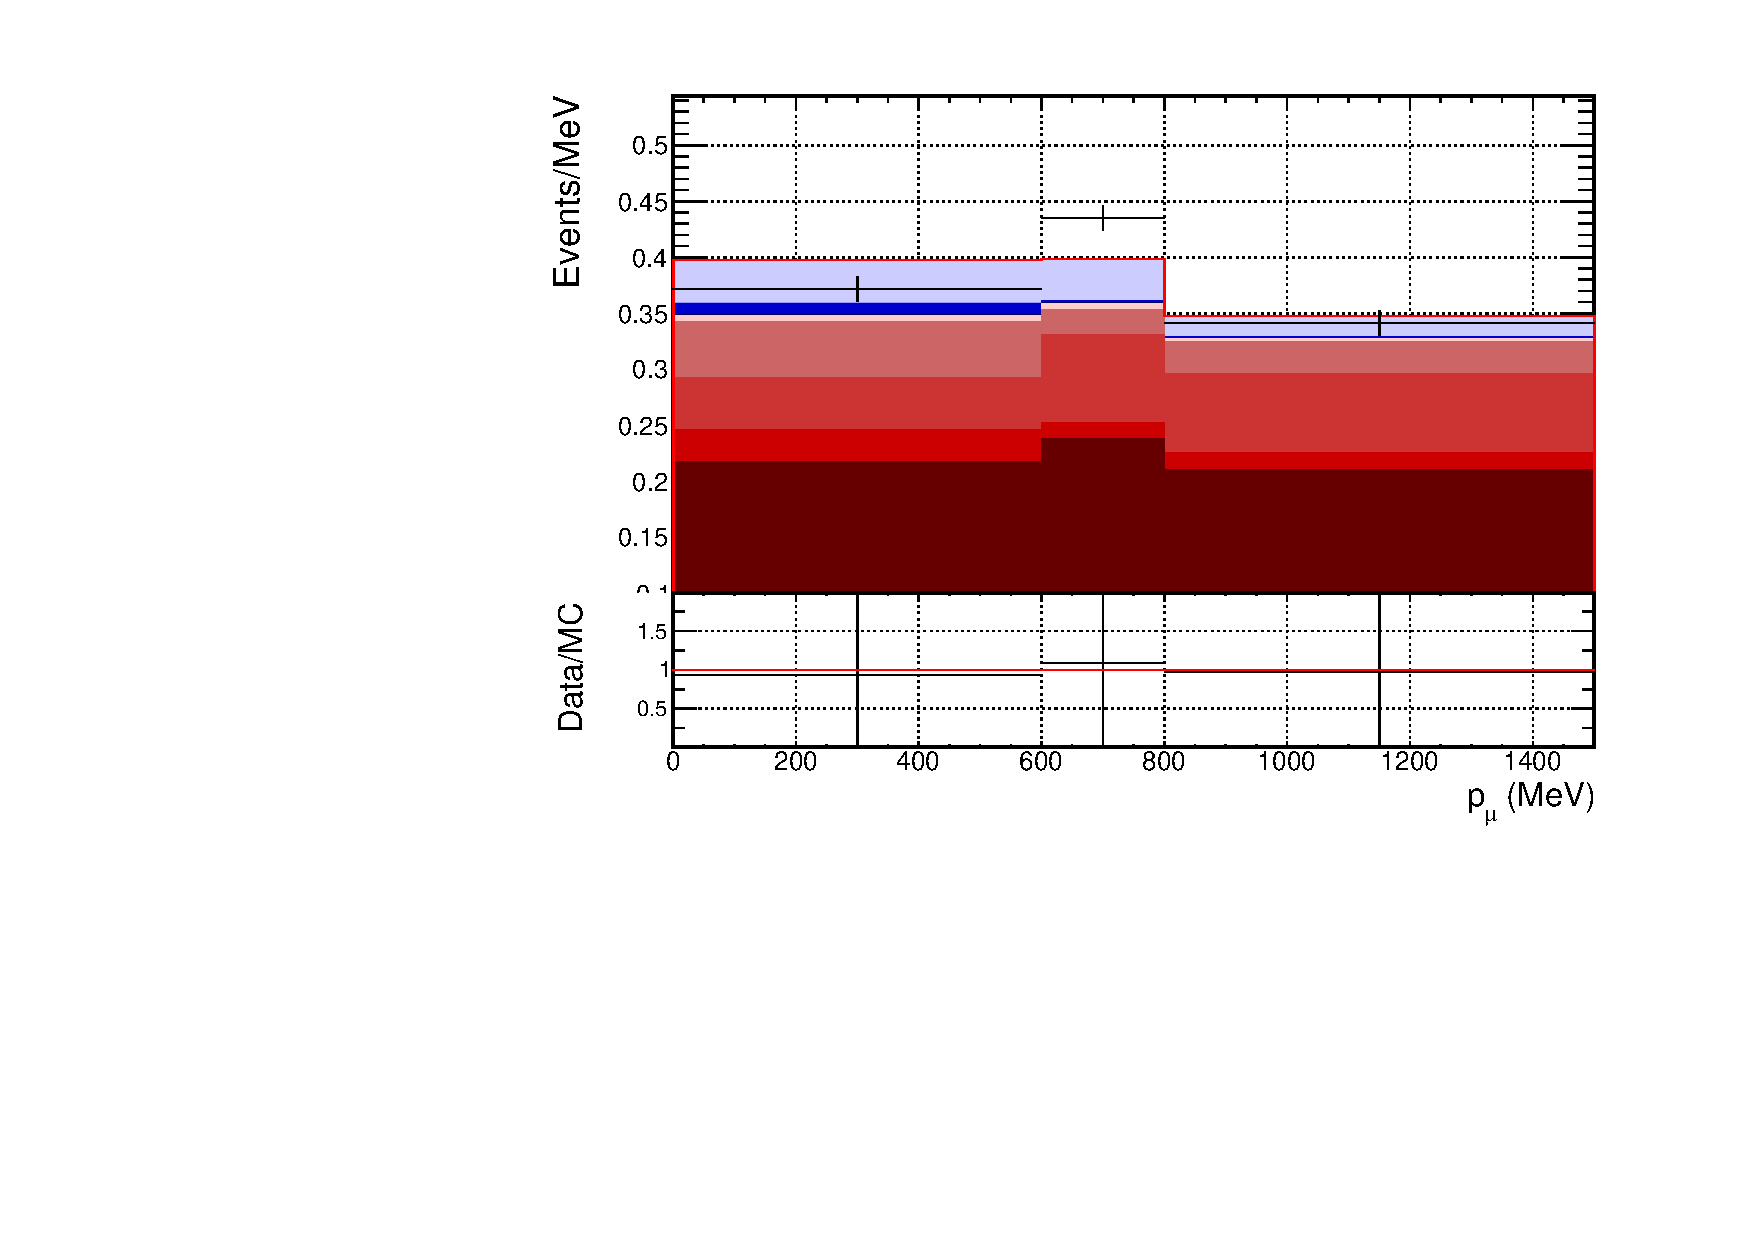
\includegraphics[width=\textwidth]{figs/FGD1_NuMuBkg_CC1pi_in_AntiNu_Mode_p}
  \caption{FGD1 RHC $\nu_{\mu}$ 1$\pi$}
\end{subfigure}
\begin{subfigure}{0.49\textwidth}
  \centering
  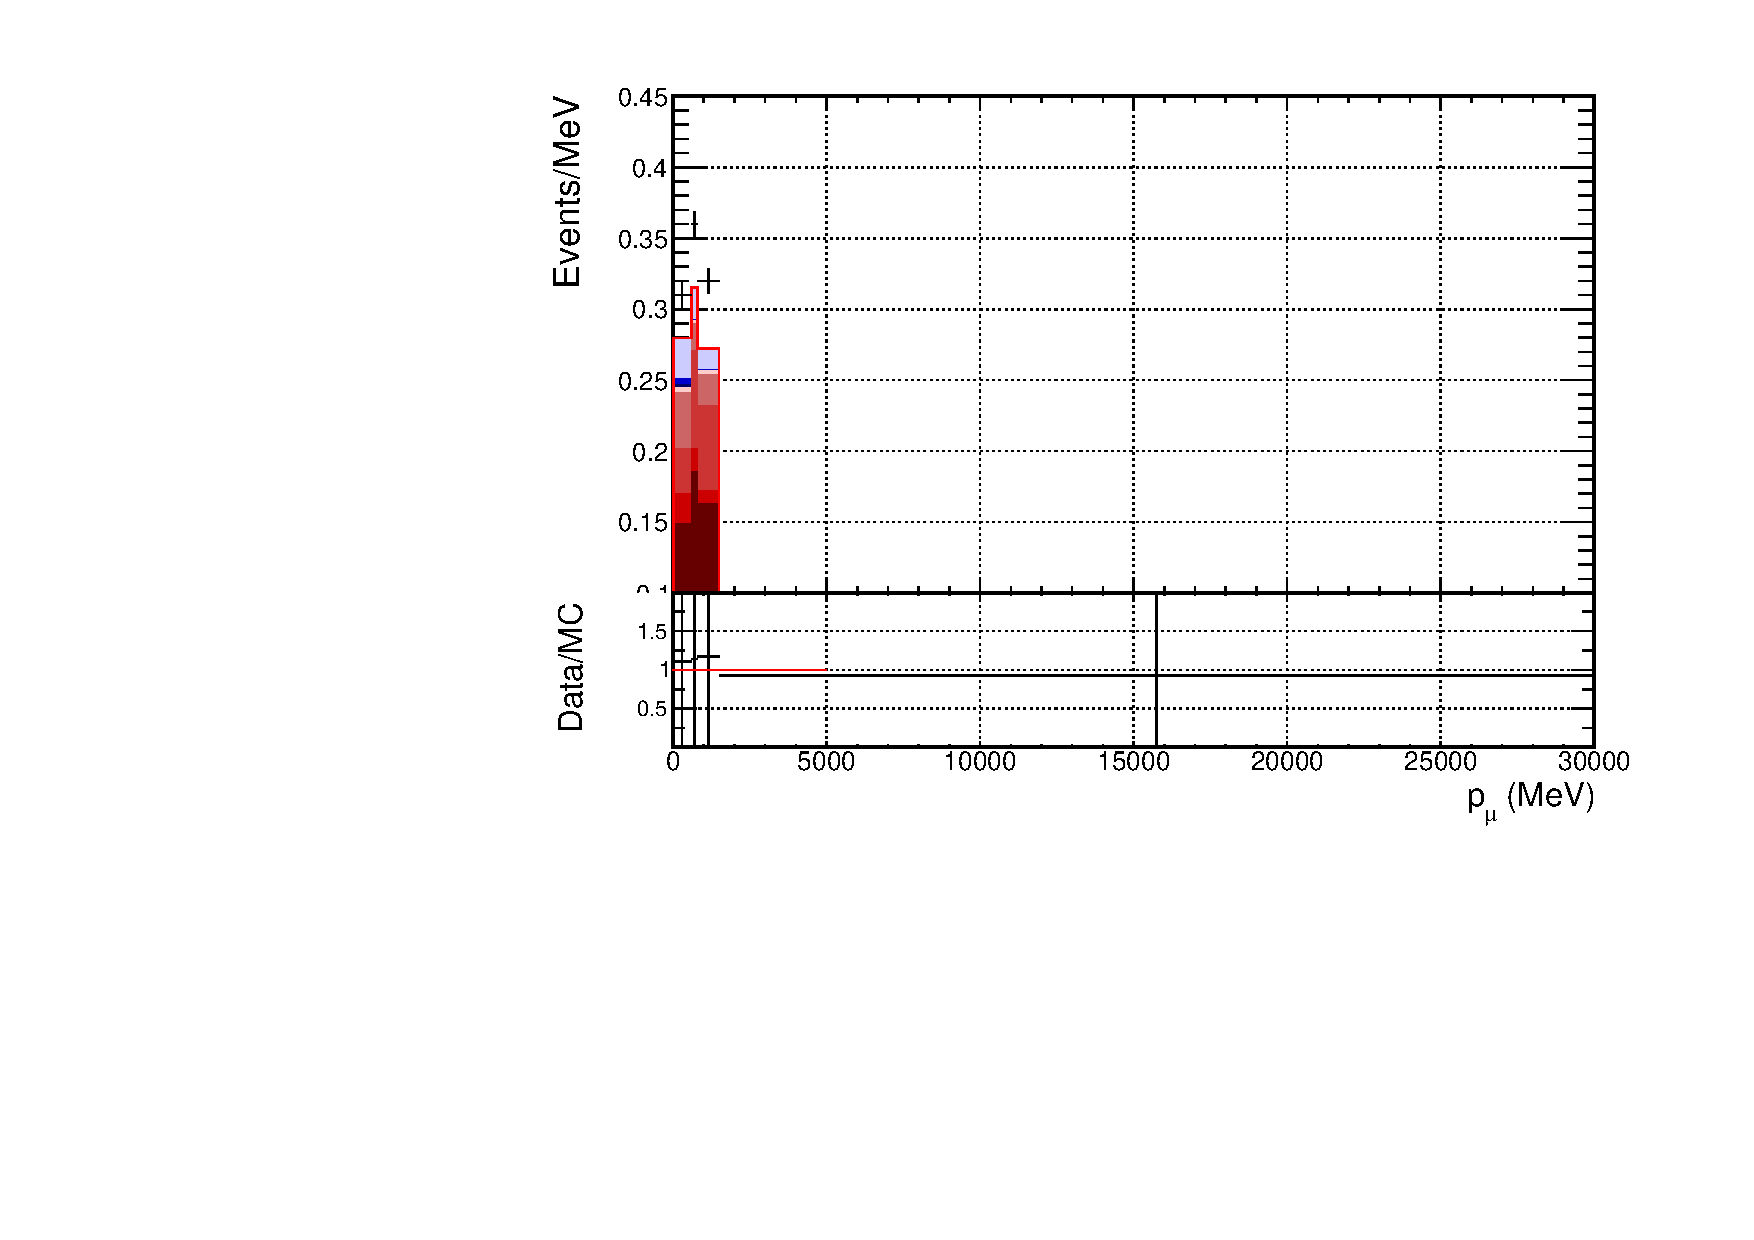
\includegraphics[width=\textwidth]{figs/FGD2_NuMuBkg_CC1pi_in_AntiNu_Mode_p}
  \caption{FGD2 RHC $\nu_{\mu}$ 1$\pi$}
\end{subfigure}

\begin{subfigure}{0.49\textwidth}
  \centering
  \includegraphics[width=\textwidth]{figs/FGD1_NuMuBkg_CCOther_in_AntiNu_Mode_p}
  \caption{FGD1 RHC $\nu_{\mu}$ Other}
\end{subfigure}
\begin{subfigure}{0.49\textwidth}
  \centering
  \includegraphics[width=\textwidth]{figs/FGD2_NuMuBkg_CCOther_in_AntiNu_Mode_p}
  \caption{FGD2 RHC $\nu_{\mu}$ Other}
\end{subfigure}
\caption{$p_{\mu}$ projections of data and nominal MC broken down by interaction mode for RHC \numu selections.}
\label{fig:pstack_rhc_numu}
\end{figure}


The projections onto the cos$\theta_{\mu}$ axis are shown in Figure \ref{fig:tstack}, along with the data and interaction mode breakdown.

The CC 0$\pi$ and CC Other samples again show oscillatory behaviour in the ratio of data to MC. At high angle, the ratio increases and decreases, but always remains $>1$. For the CC 1$\pi$ samples,  the ratio is more flat, but at high angle oscillates between the MC over and underestimating the data. The behaviour is consistent across the FGDs.

\begin{figure}[!h]
\centering
\begin{subfigure}{.24\textwidth}
  \centering
  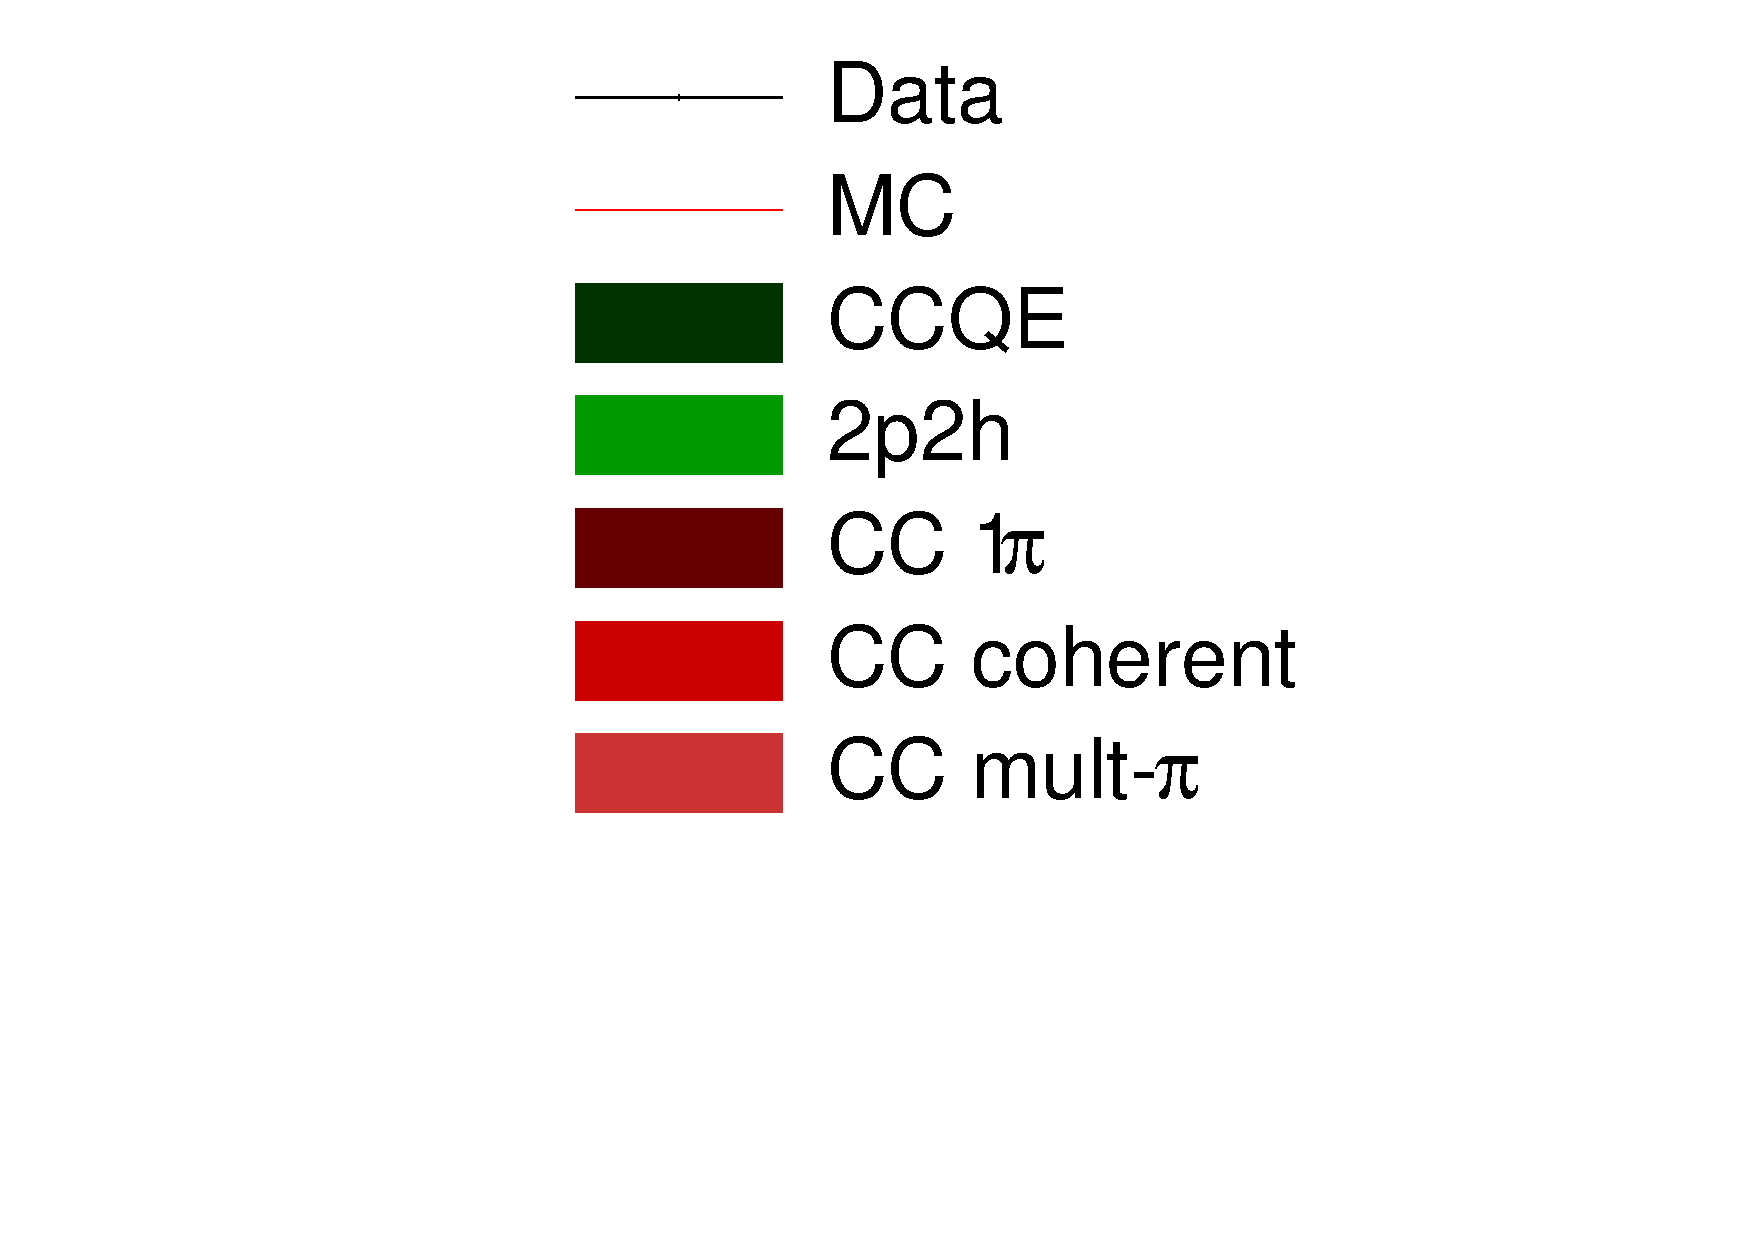
\includegraphics[width=\linewidth, trim={5mm 60mm 30mm 0mm}, clip]{figs/legend}
\end{subfigure}
\begin{subfigure}{.24\textwidth}
  \centering
  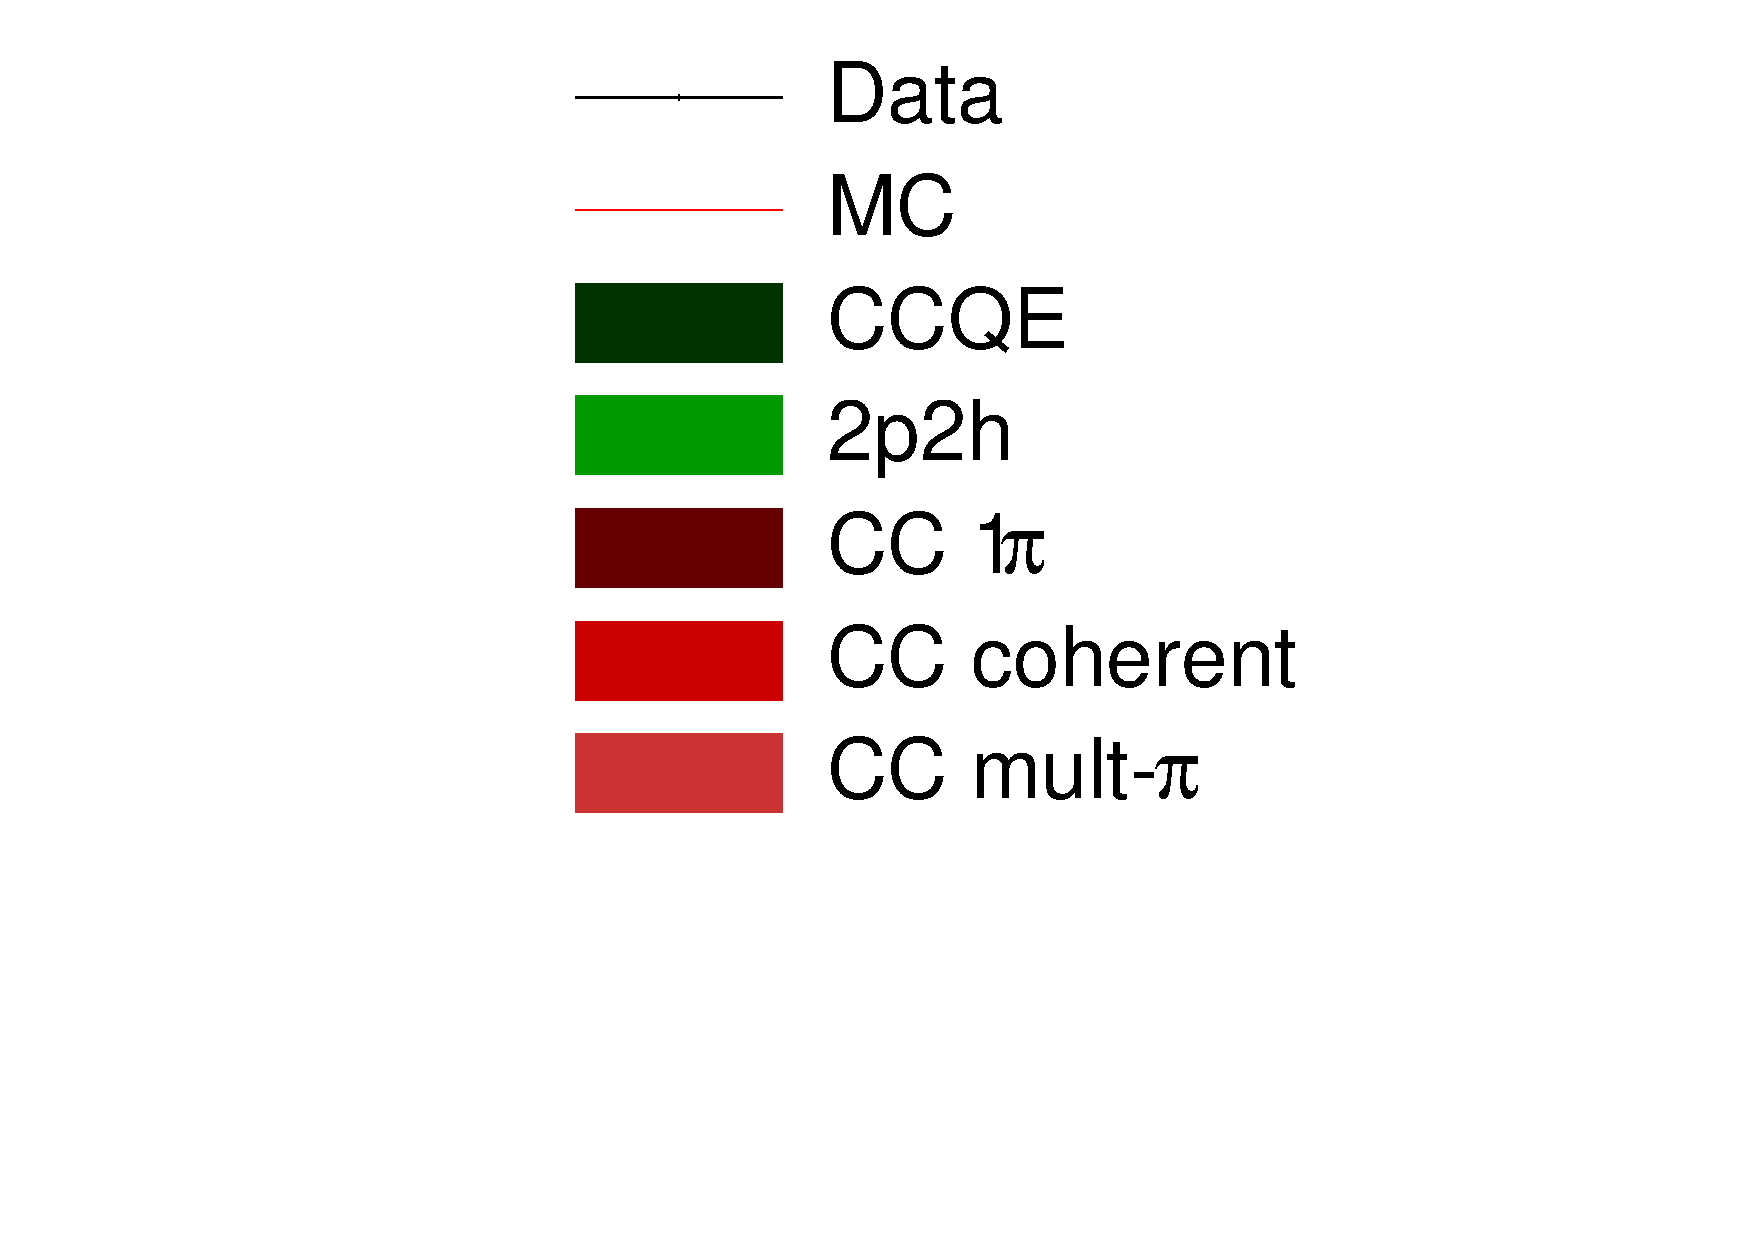
\includegraphics[width=\linewidth, trim={5mm 0mm 30mm 80mm}, clip]{figs/legend}
\end{subfigure}
\begin{subfigure}{.24\textwidth}
  \centering
  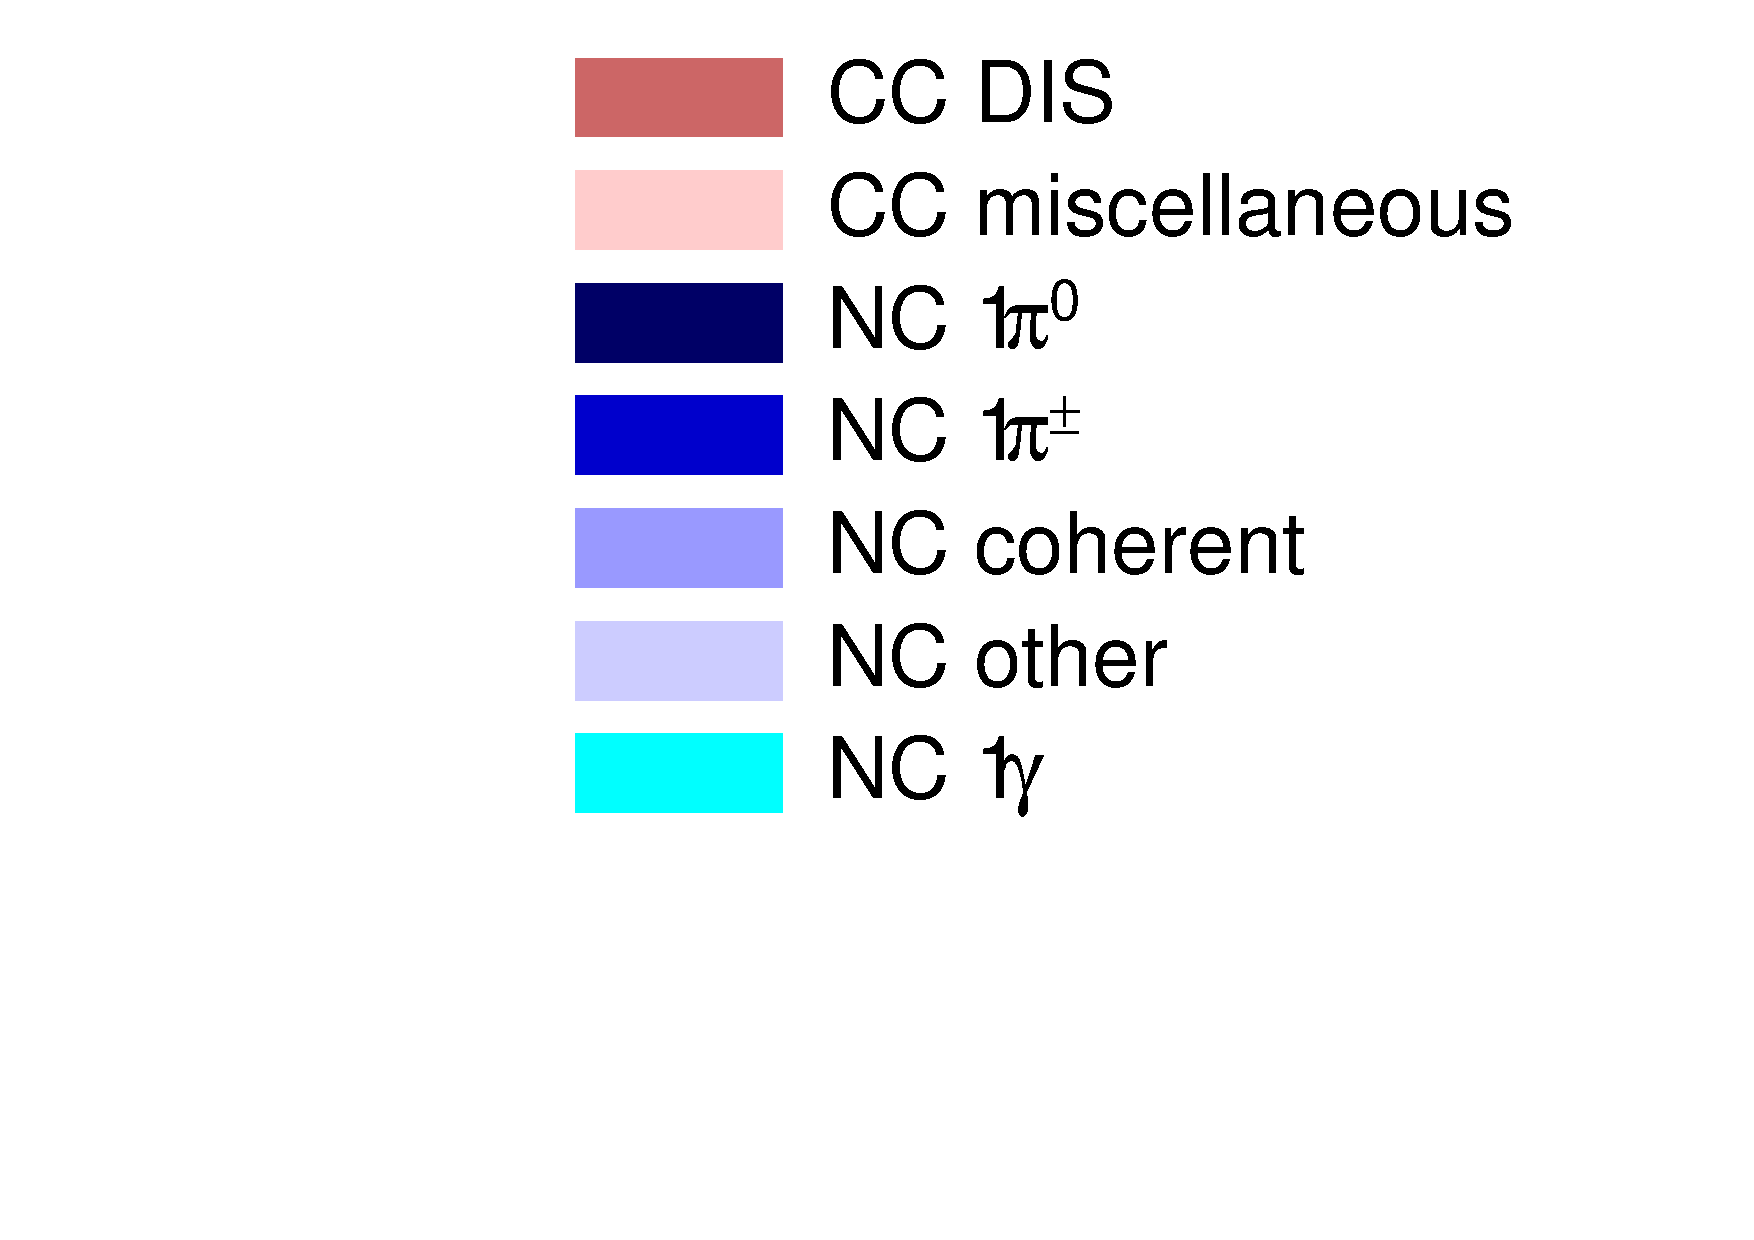
\includegraphics[width=\linewidth, trim={5mm 60mm 30mm 0mm}, clip]{figs/legend2}
\end{subfigure}
\begin{subfigure}{.24\textwidth}
  \centering
  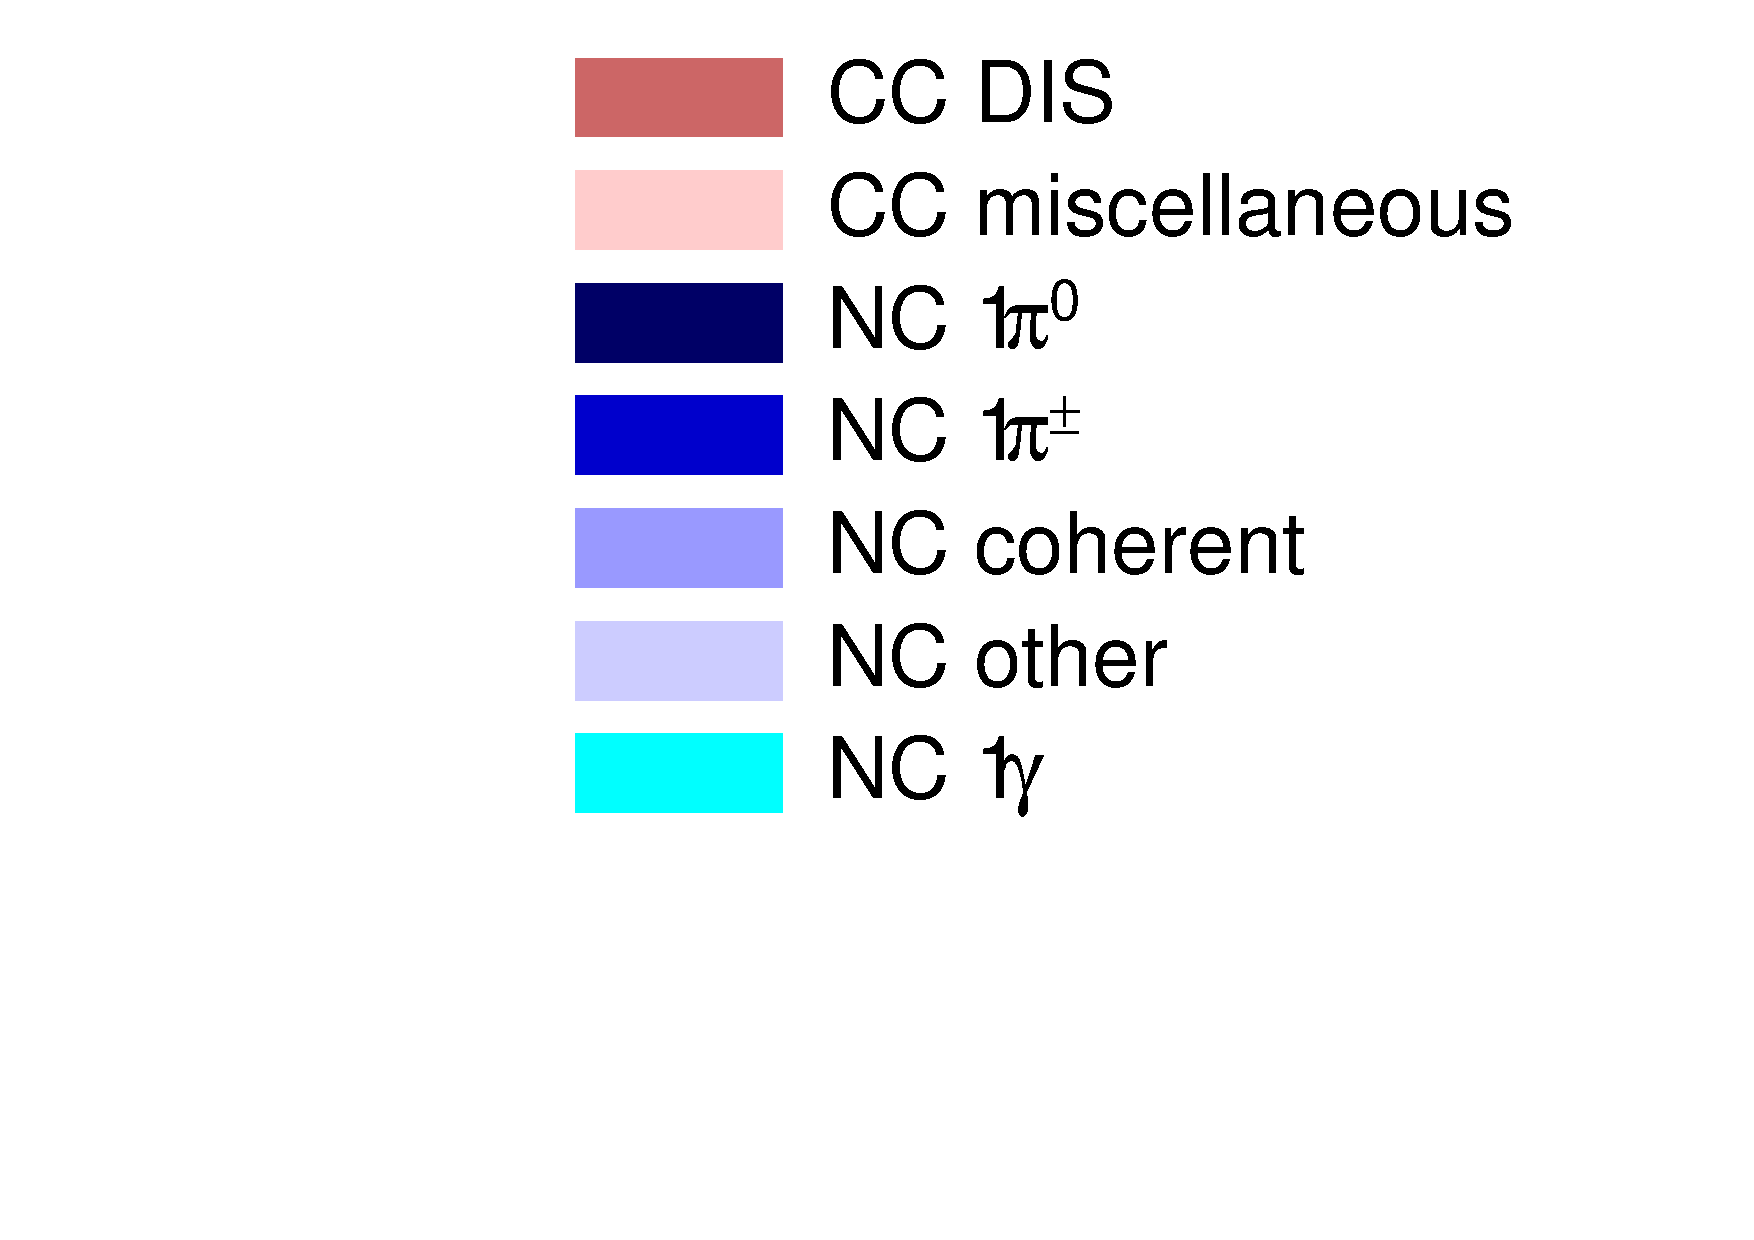
\includegraphics[width=\linewidth, trim={5mm 0mm 30mm 80mm}, clip]{figs/legend2}
\end{subfigure}

\begin{subfigure}{0.49\textwidth}
  \centering
  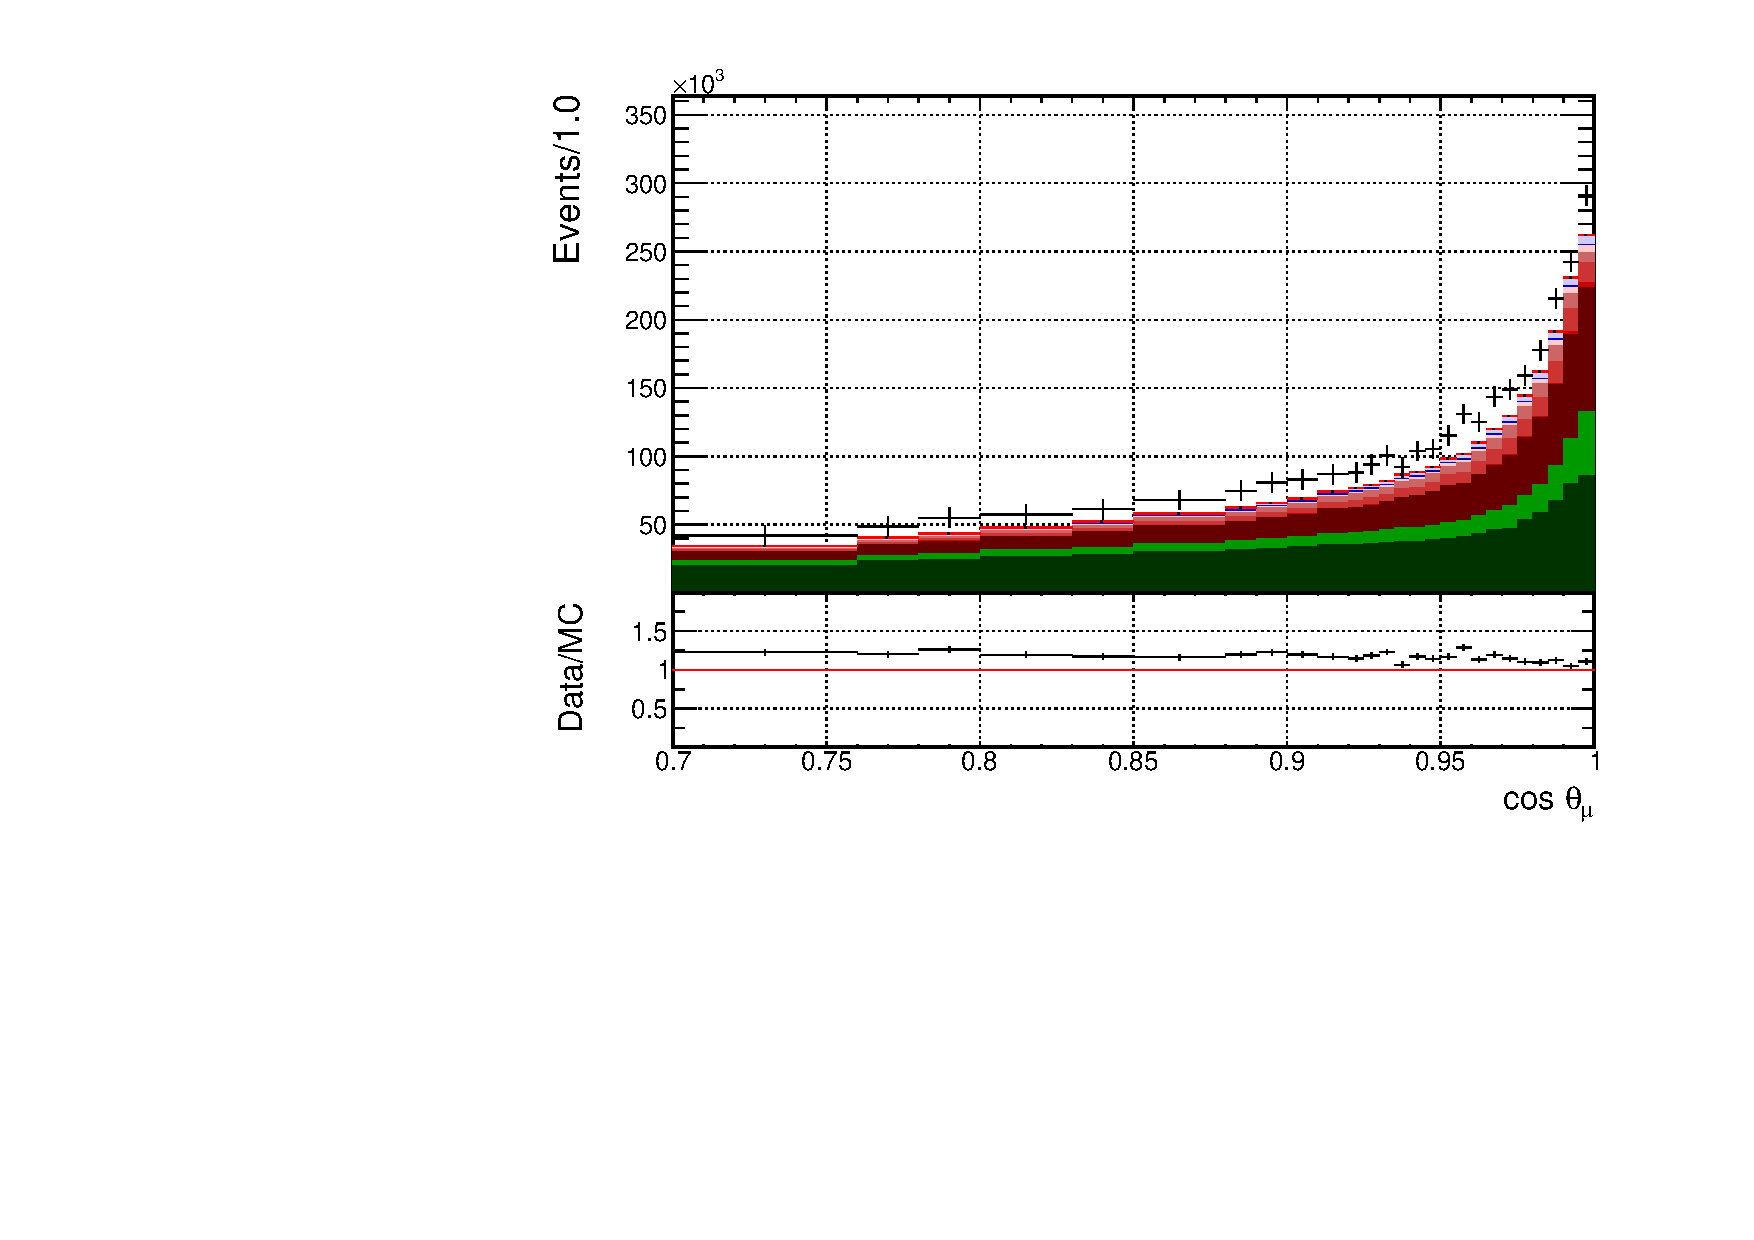
\includegraphics[width=\textwidth]{figs/FGD1_numuCC_0pi_t}
  \caption{FGD1 FHC $\nu_{\mu}$ 0$\pi$}
\end{subfigure}
\begin{subfigure}{0.49\textwidth}
  \centering
  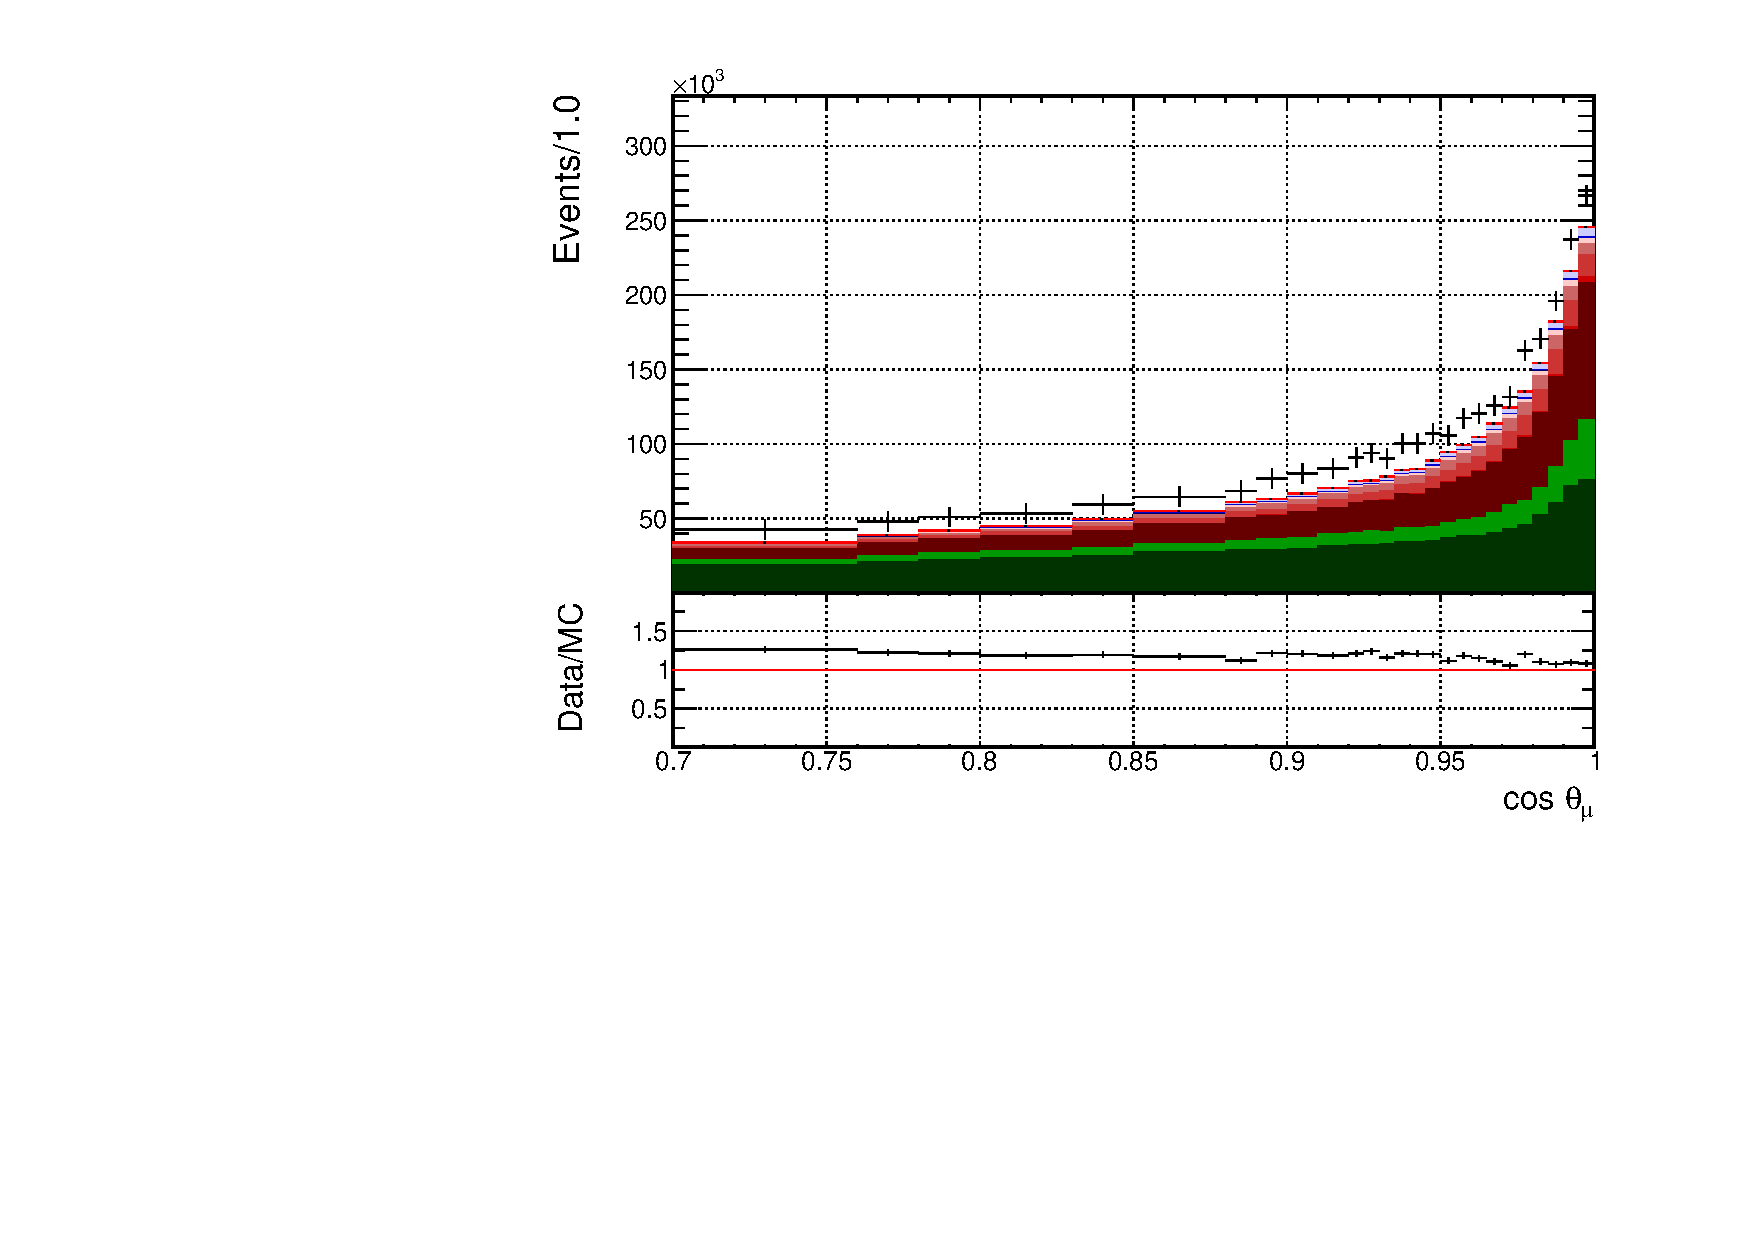
\includegraphics[width=\textwidth]{figs/FGD2_numuCC_0pi_t}
  \caption{FGD2 FHC $\nu_{\mu}$ 0$\pi$}
\end{subfigure}

\begin{subfigure}{0.49\textwidth}
  \centering
  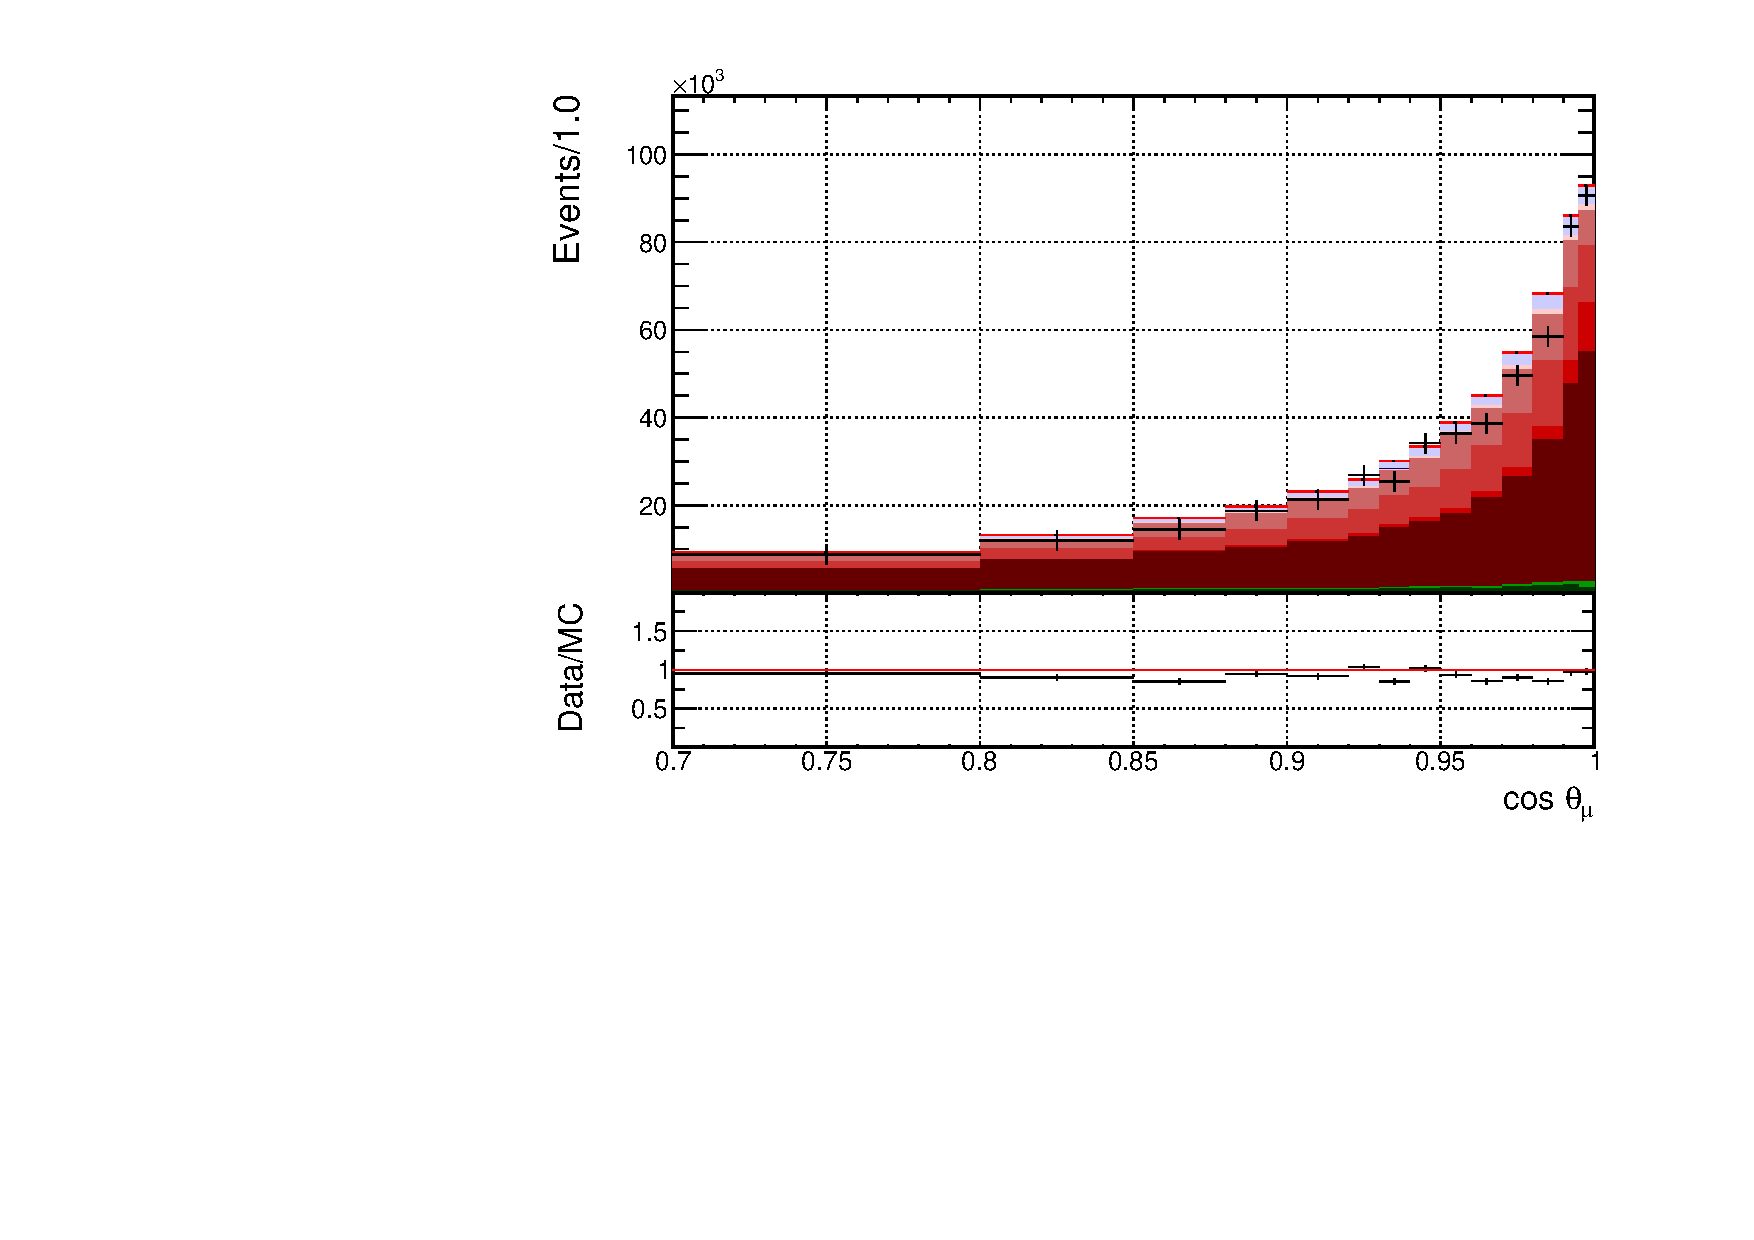
\includegraphics[width=\textwidth]{figs/FGD1_numuCC_1pi_t}
  \caption{FGD1 FHC $\nu_{\mu}$ 1$\pi$}
\end{subfigure}
\centering
\begin{subfigure}{0.49\textwidth}
  \centering
  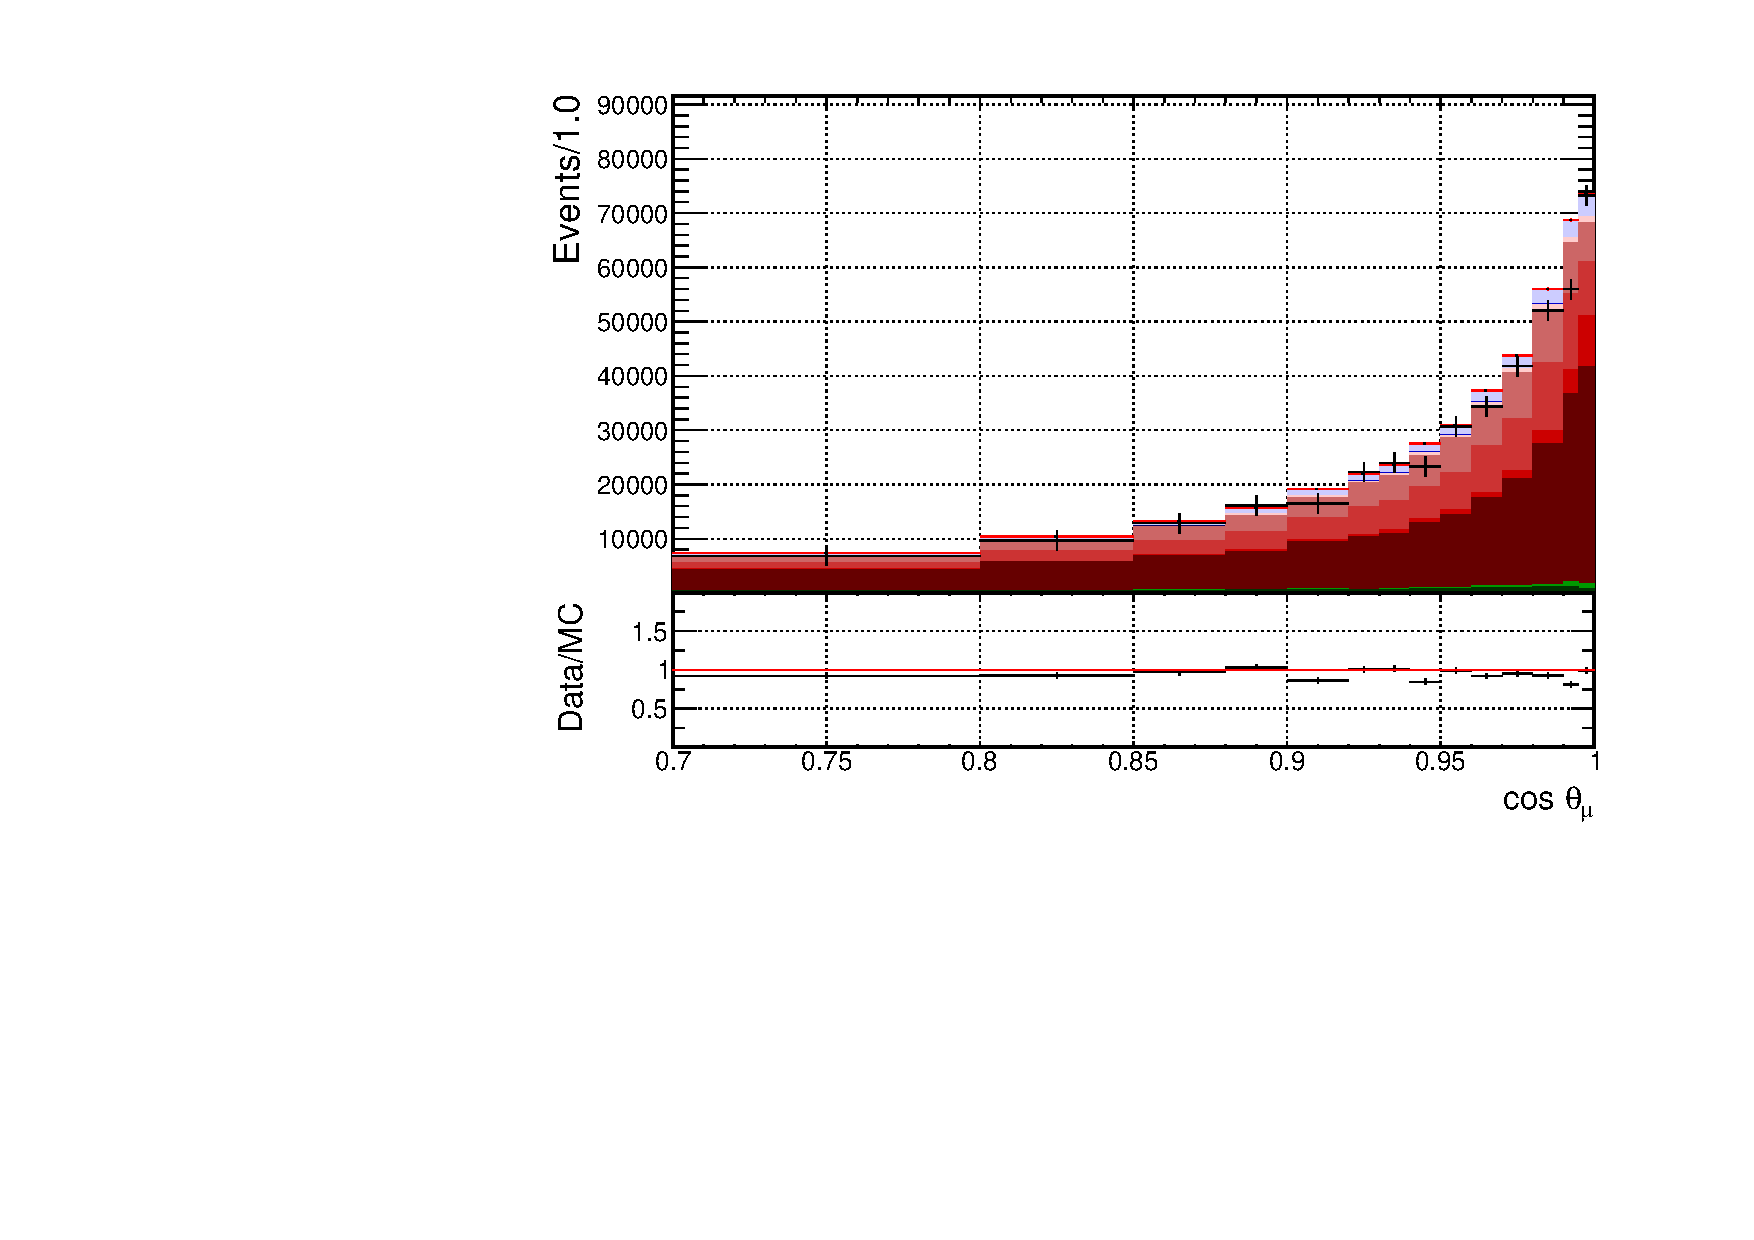
\includegraphics[width=\textwidth]{figs/FGD2_numuCC_1pi_t}
  \caption{FGD2 FHC $\nu_{\mu}$ 1$\pi$}
\end{subfigure}

\begin{subfigure}{0.49\textwidth}
  \centering
  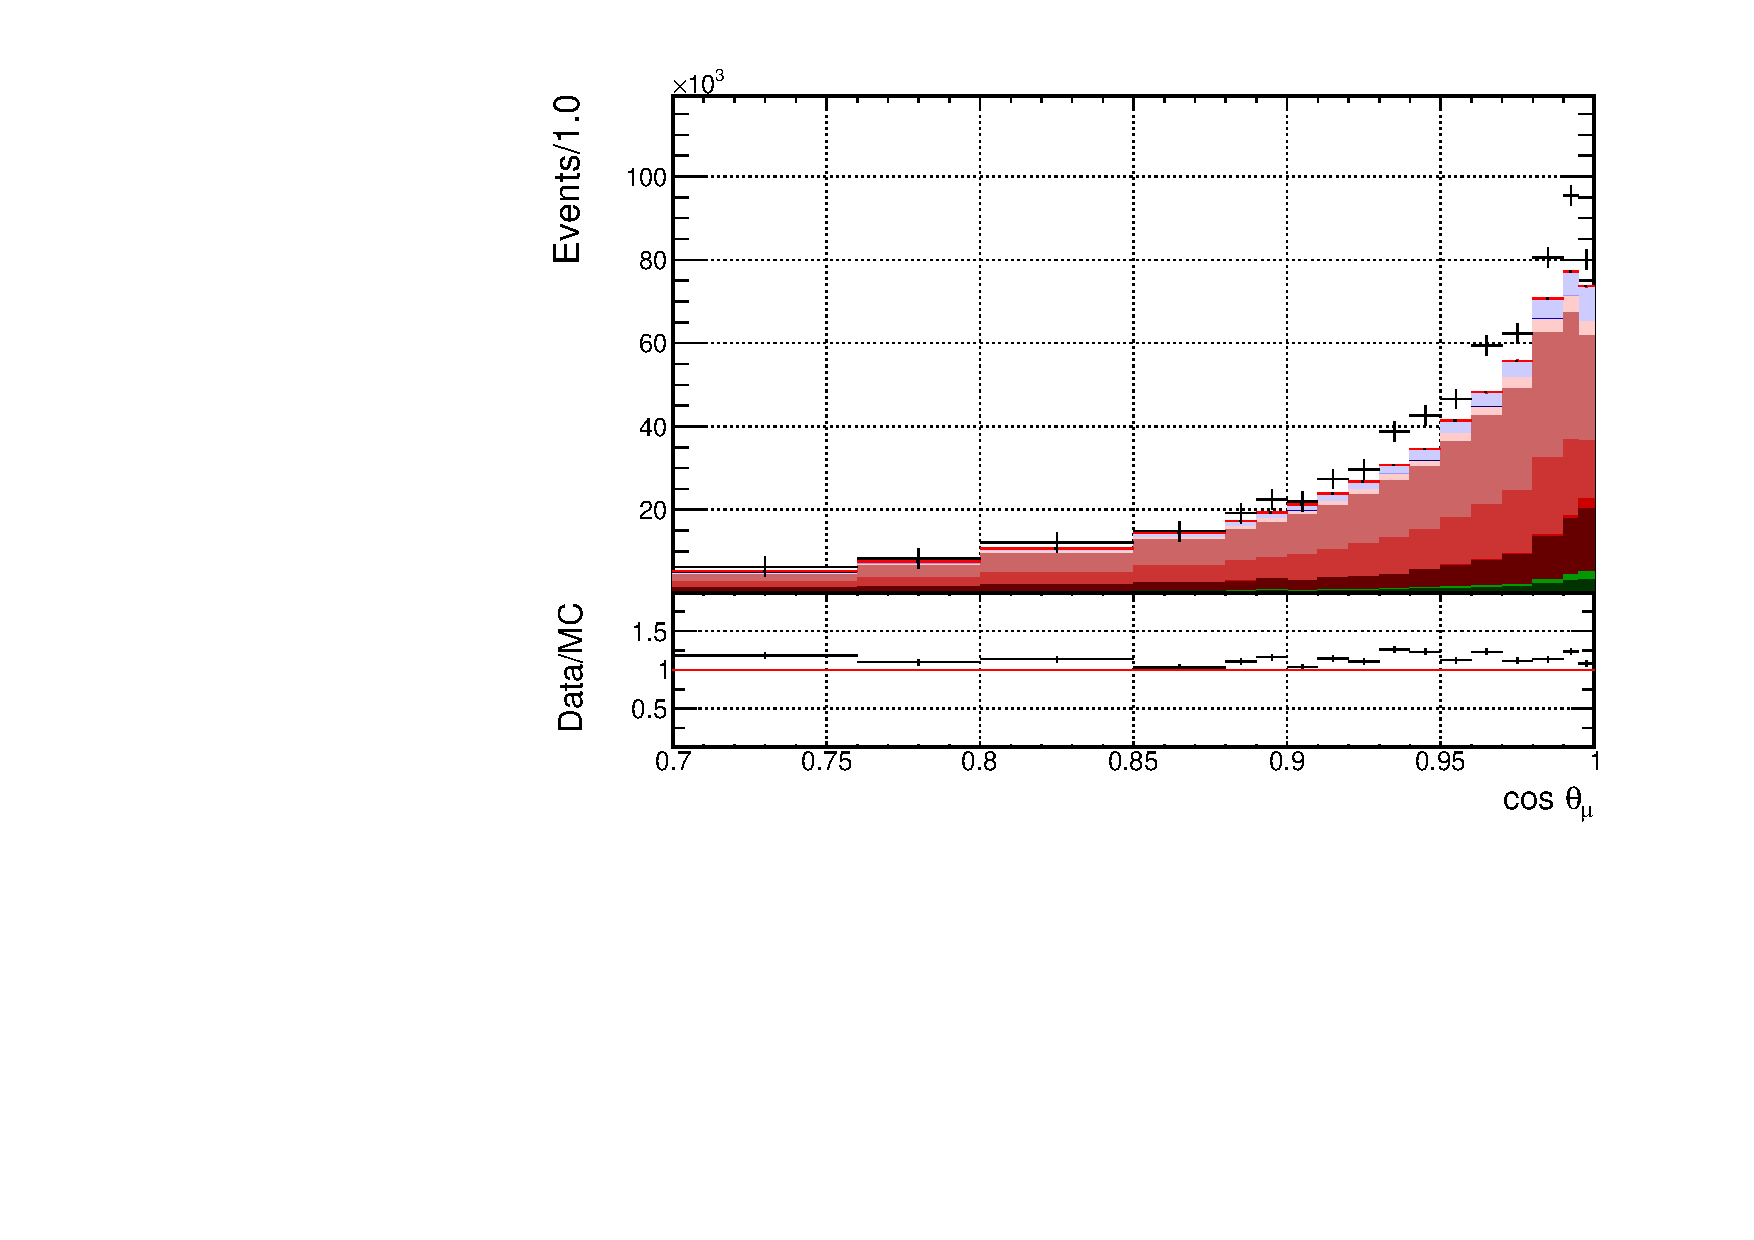
\includegraphics[width=\textwidth]{figs/FGD1_numuCC_other_t}
  \caption{FGD1 FHC $\nu_{\mu}$ Other}
\end{subfigure}
\begin{subfigure}{0.49\textwidth}
  \centering
  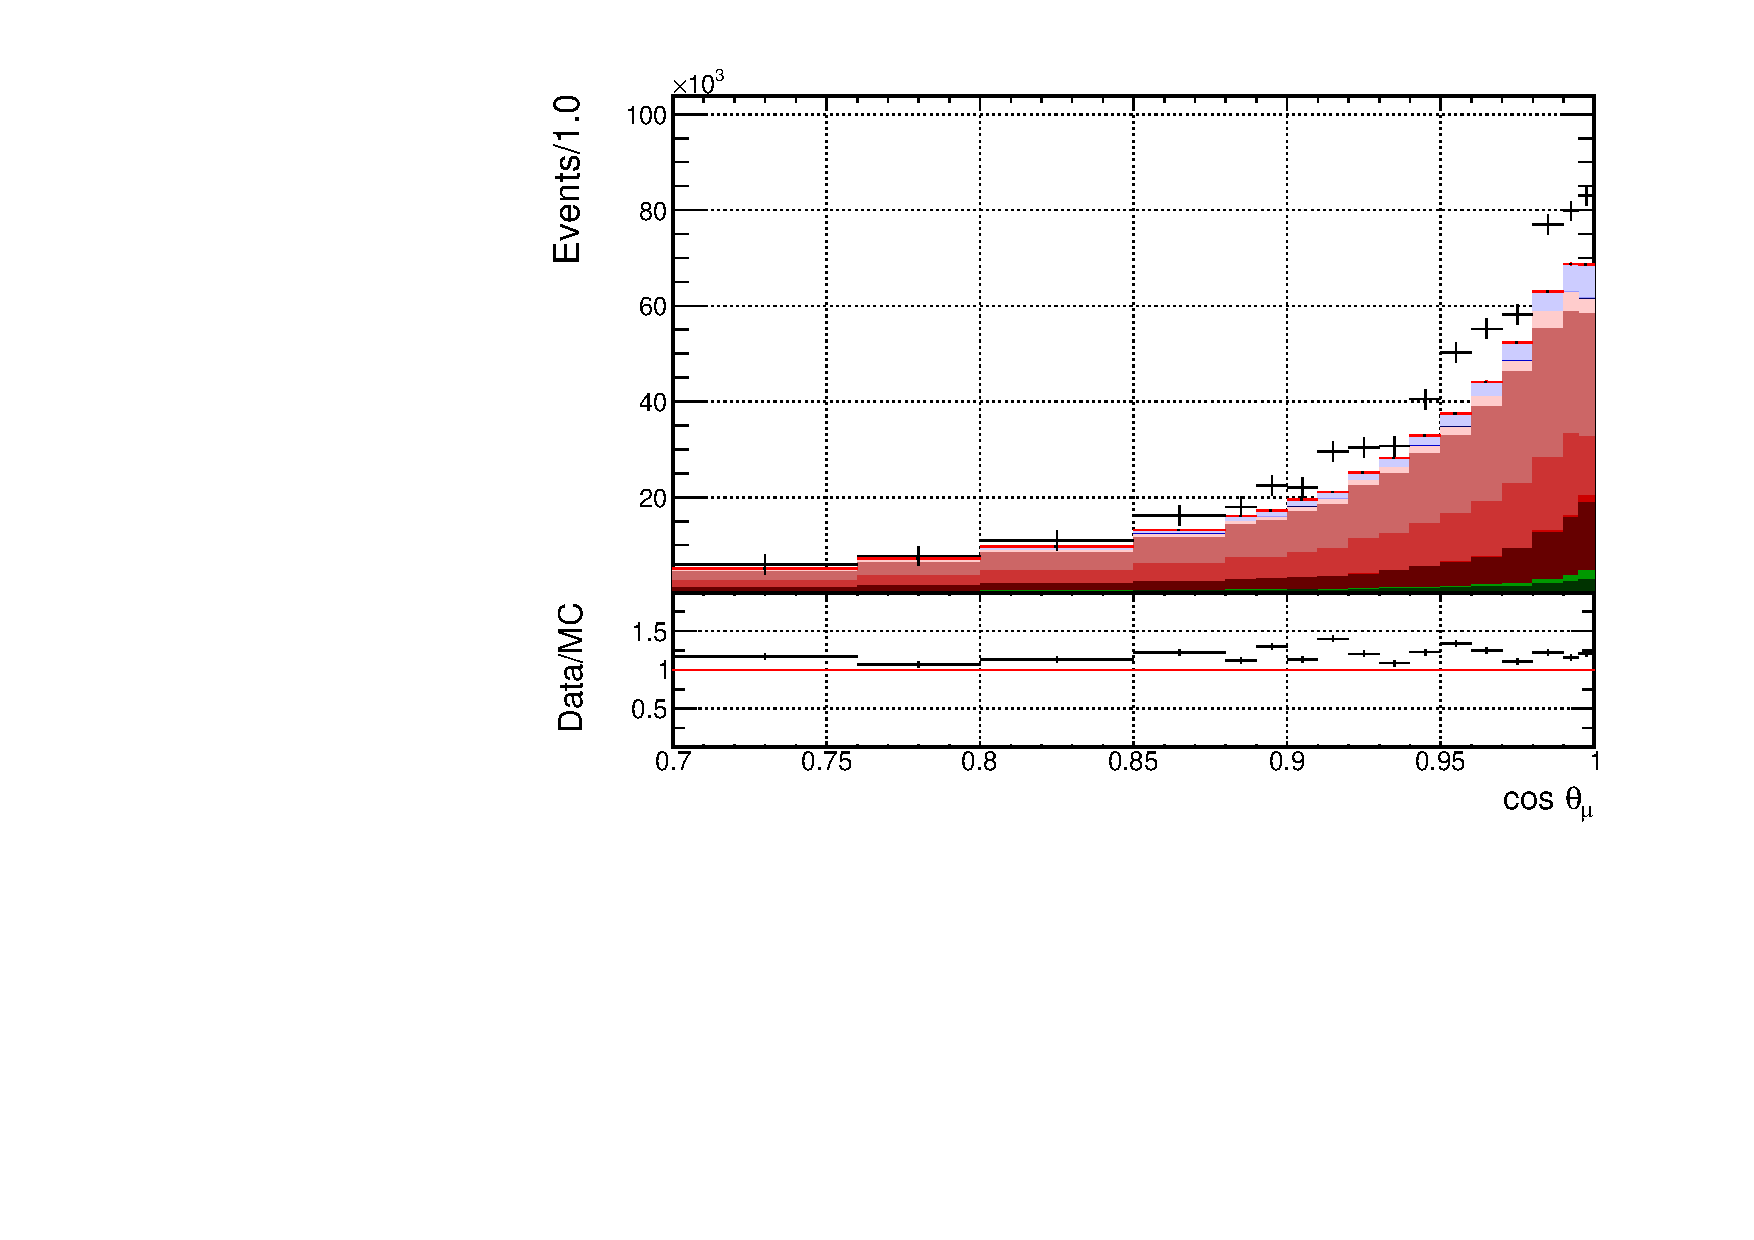
\includegraphics[width=\textwidth]{figs/FGD2_numuCC_other_t}
  \caption{FGD2 $\nu_{\mu}$ Other}
\end{subfigure}
\caption{$\cos\theta_{\mu}$ projections of data and nominal MC broken down by interaction mode for FHC selections.}
\label{fig:tstack_fhc}
\end{figure}

\begin{figure}[!h]
\centering
\begin{subfigure}{.24\textwidth}
  \centering
  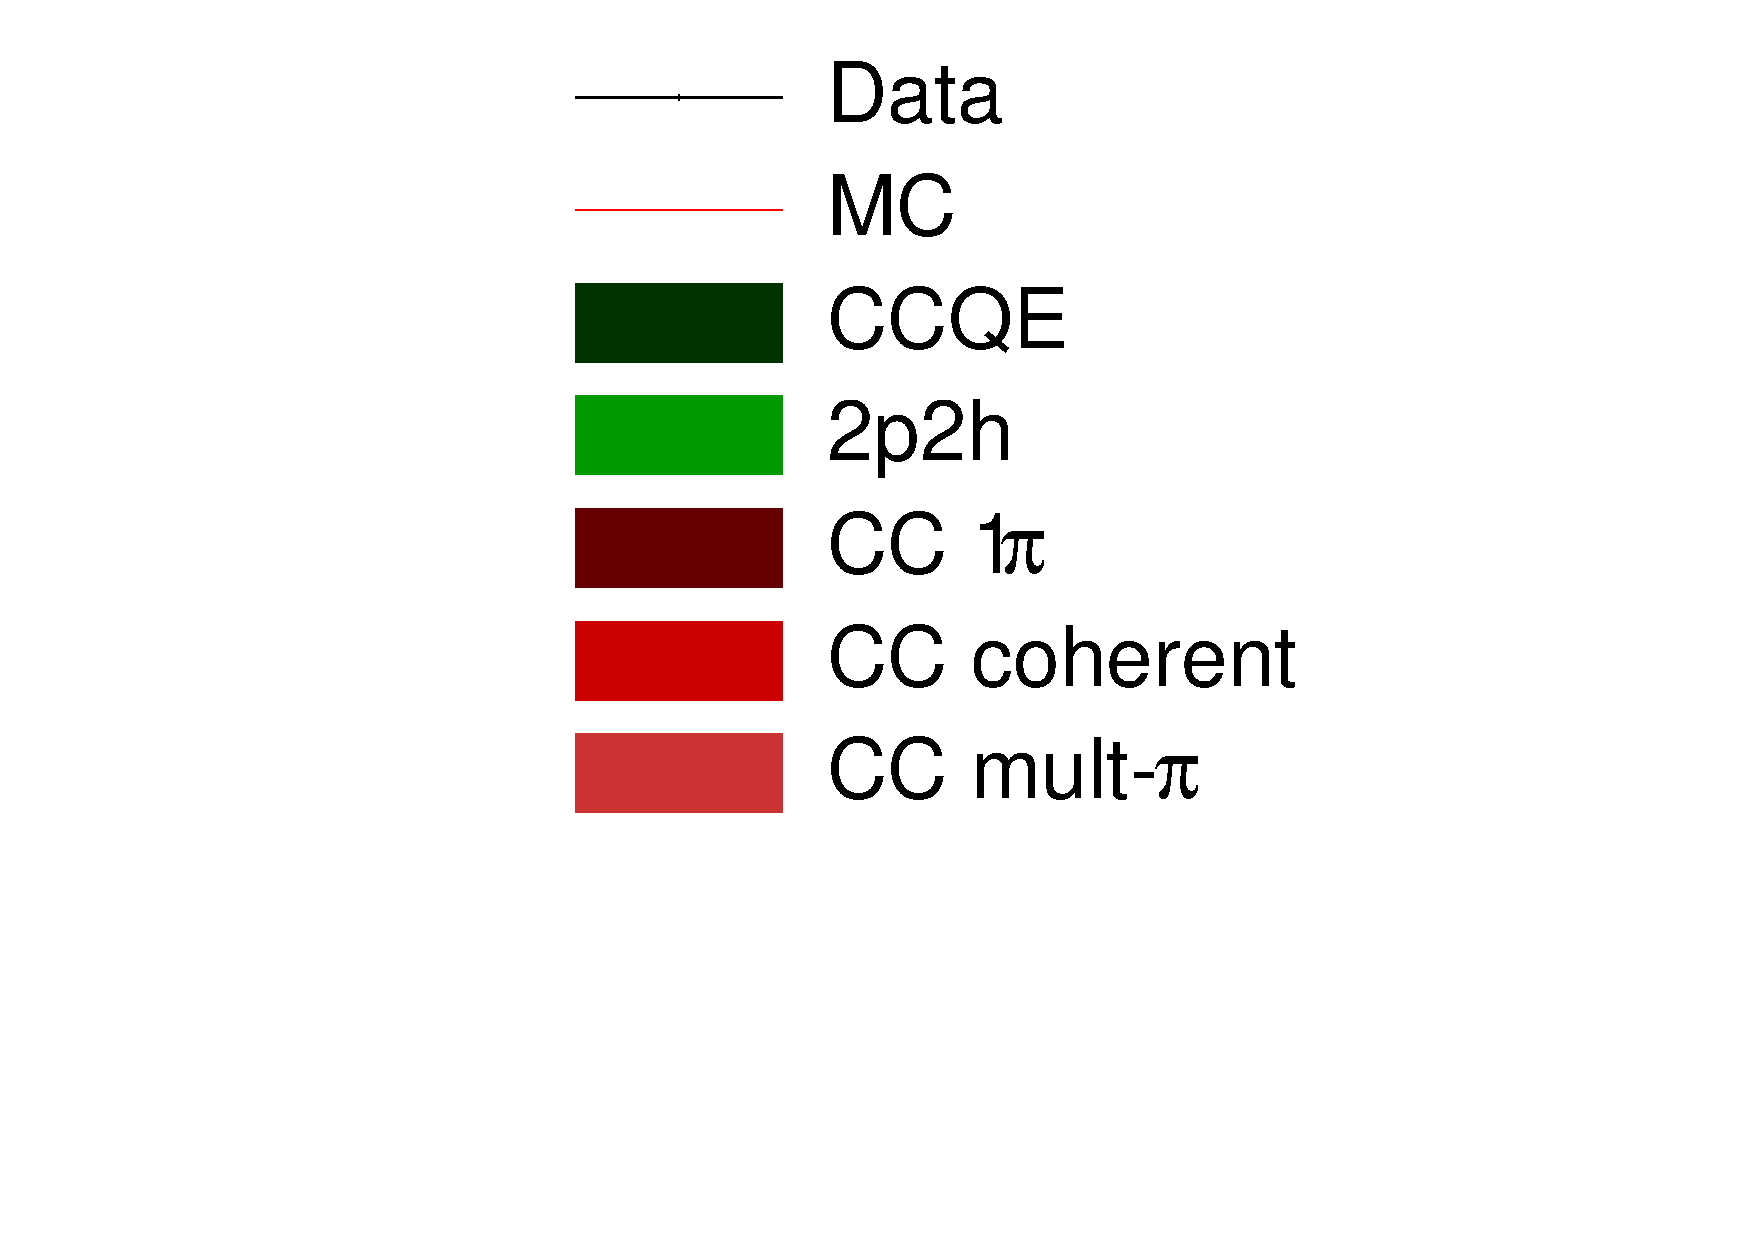
\includegraphics[width=\linewidth, trim={5mm 60mm 30mm 0mm}, clip]{figs/legend}
\end{subfigure}
\begin{subfigure}{.24\textwidth}
  \centering
  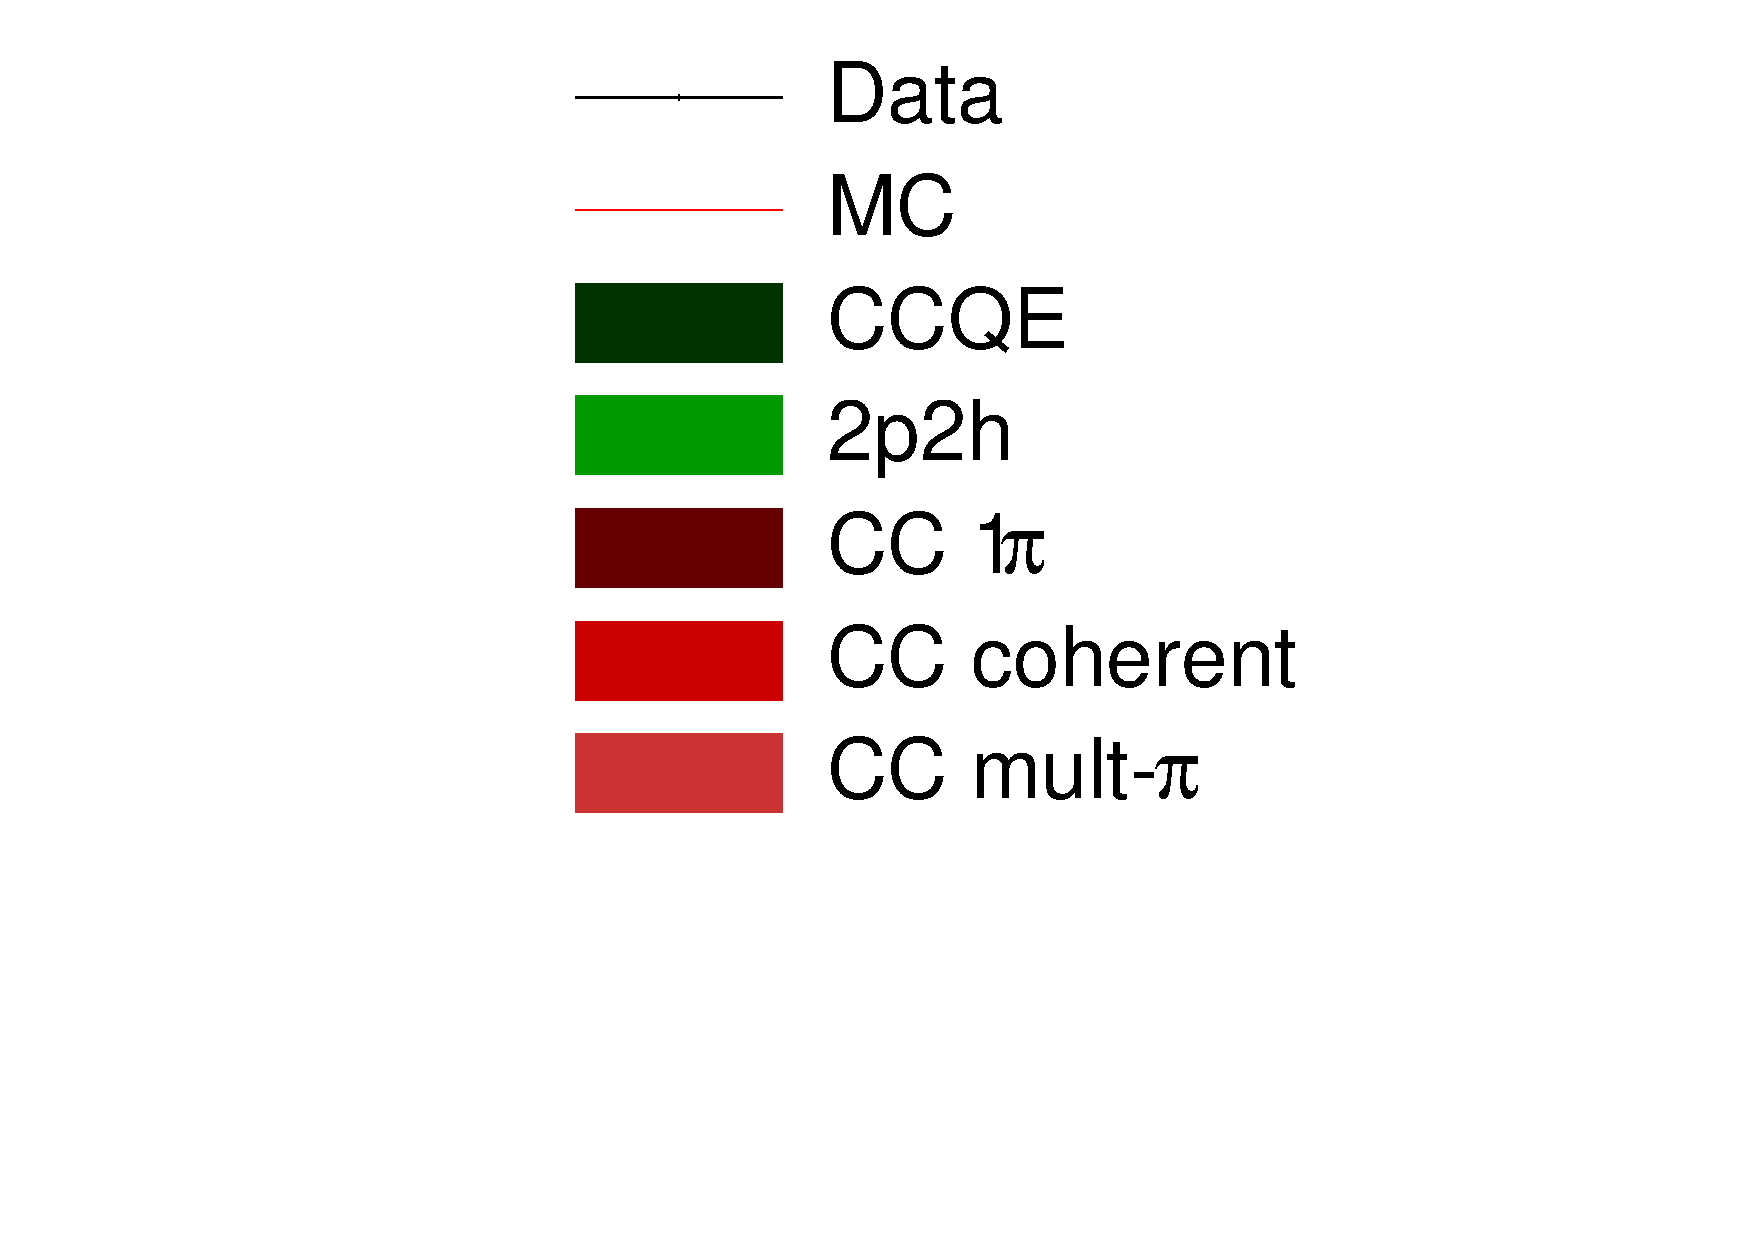
\includegraphics[width=\linewidth, trim={5mm 0mm 30mm 80mm}, clip]{figs/legend}
\end{subfigure}
\begin{subfigure}{.24\textwidth}
  \centering
  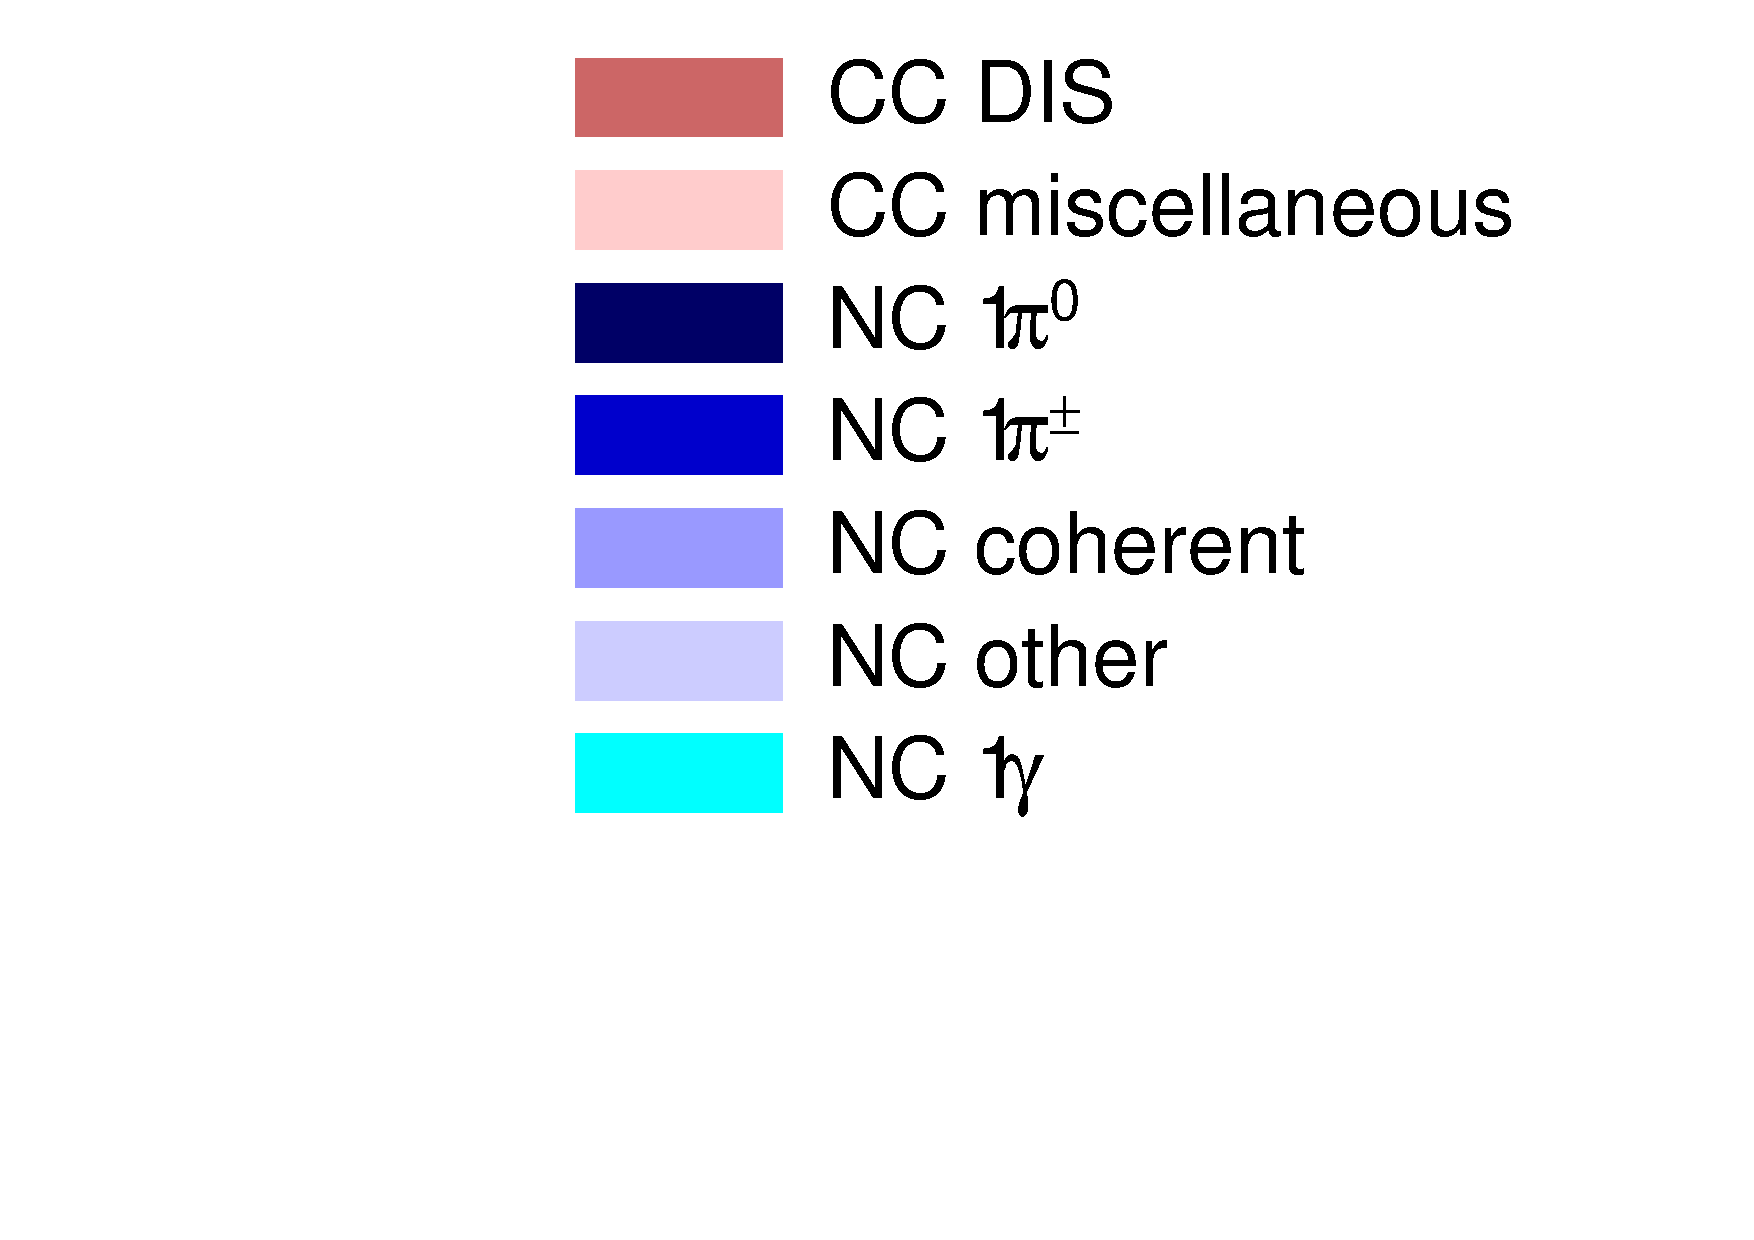
\includegraphics[width=\linewidth, trim={5mm 60mm 30mm 0mm}, clip]{figs/legend2}
\end{subfigure}
\begin{subfigure}{.24\textwidth}
  \centering
  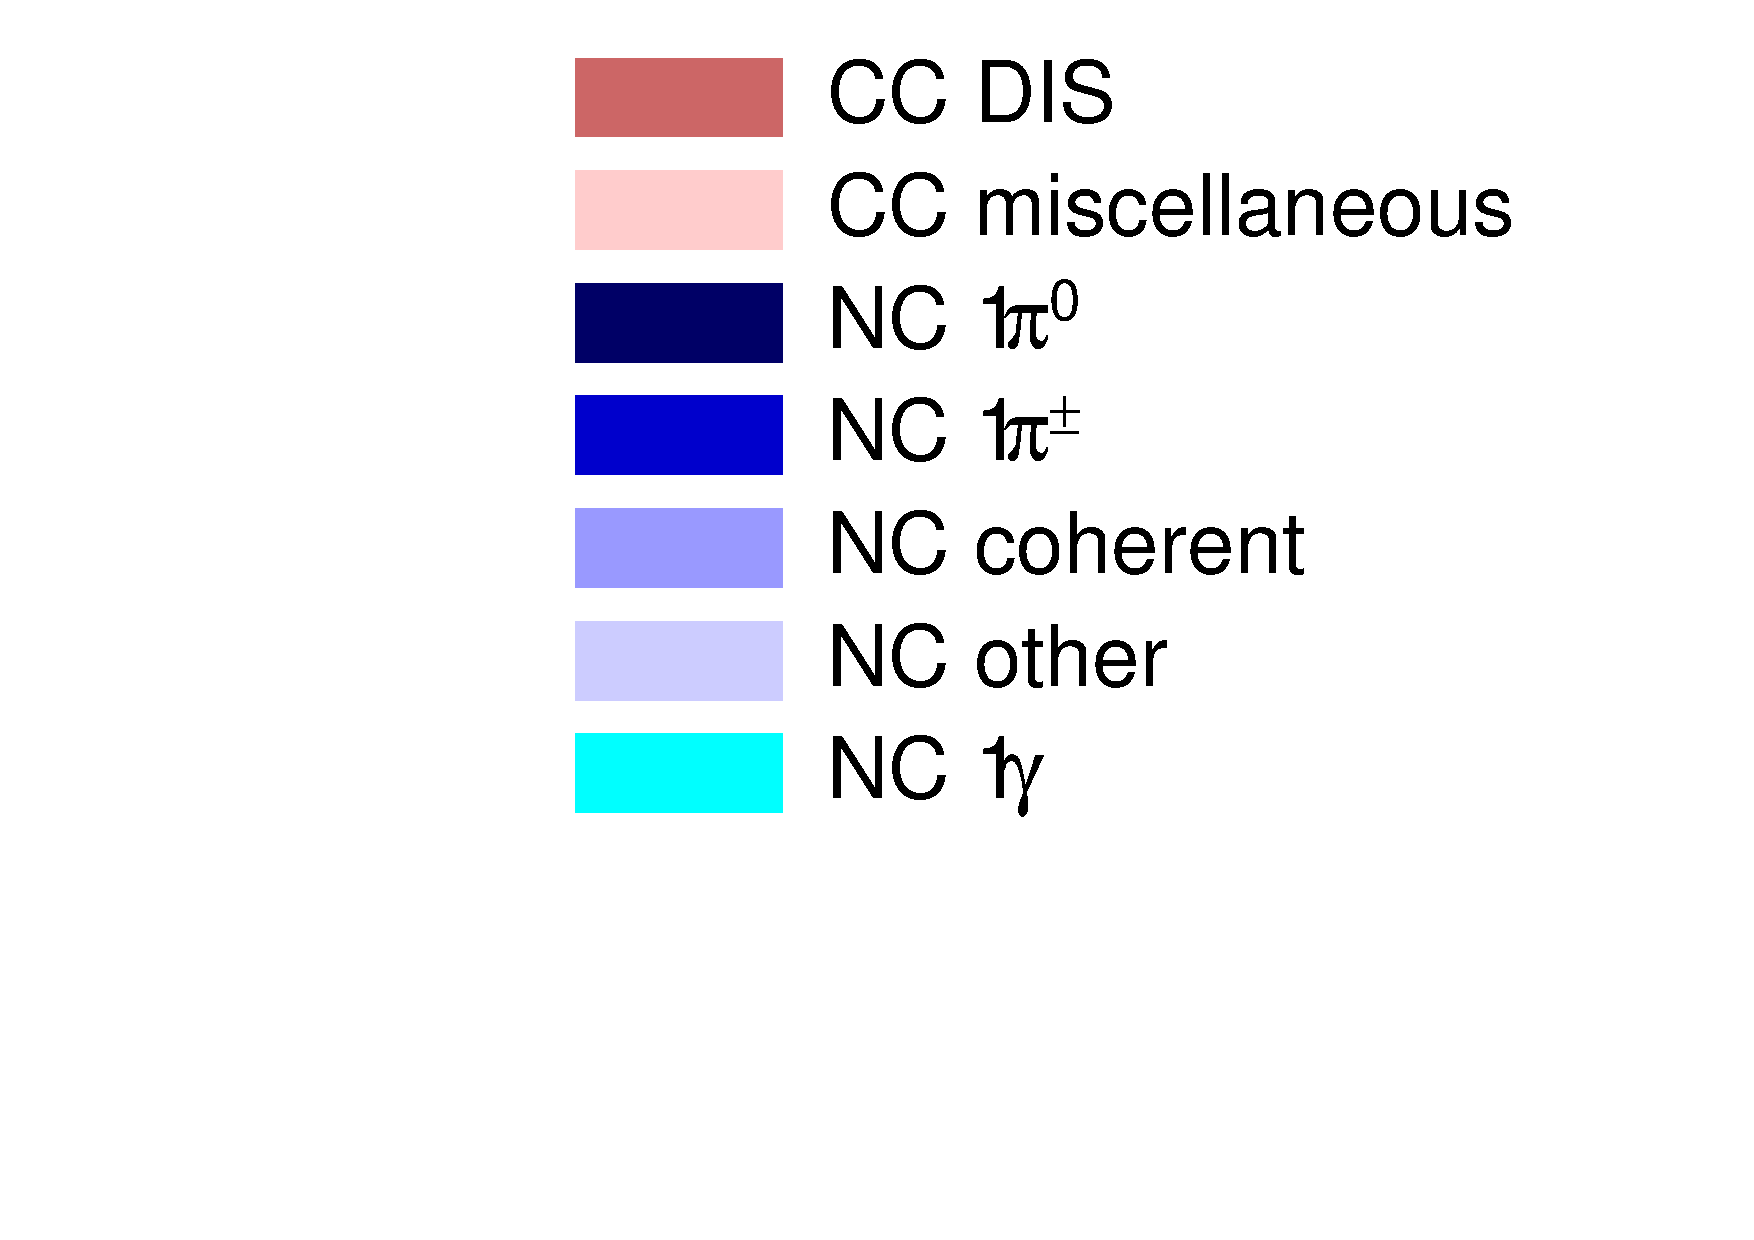
\includegraphics[width=\linewidth, trim={5mm 0mm 30mm 80mm}, clip]{figs/legend2}
\end{subfigure}

\begin{subfigure}{0.49\textwidth}
  \centering
  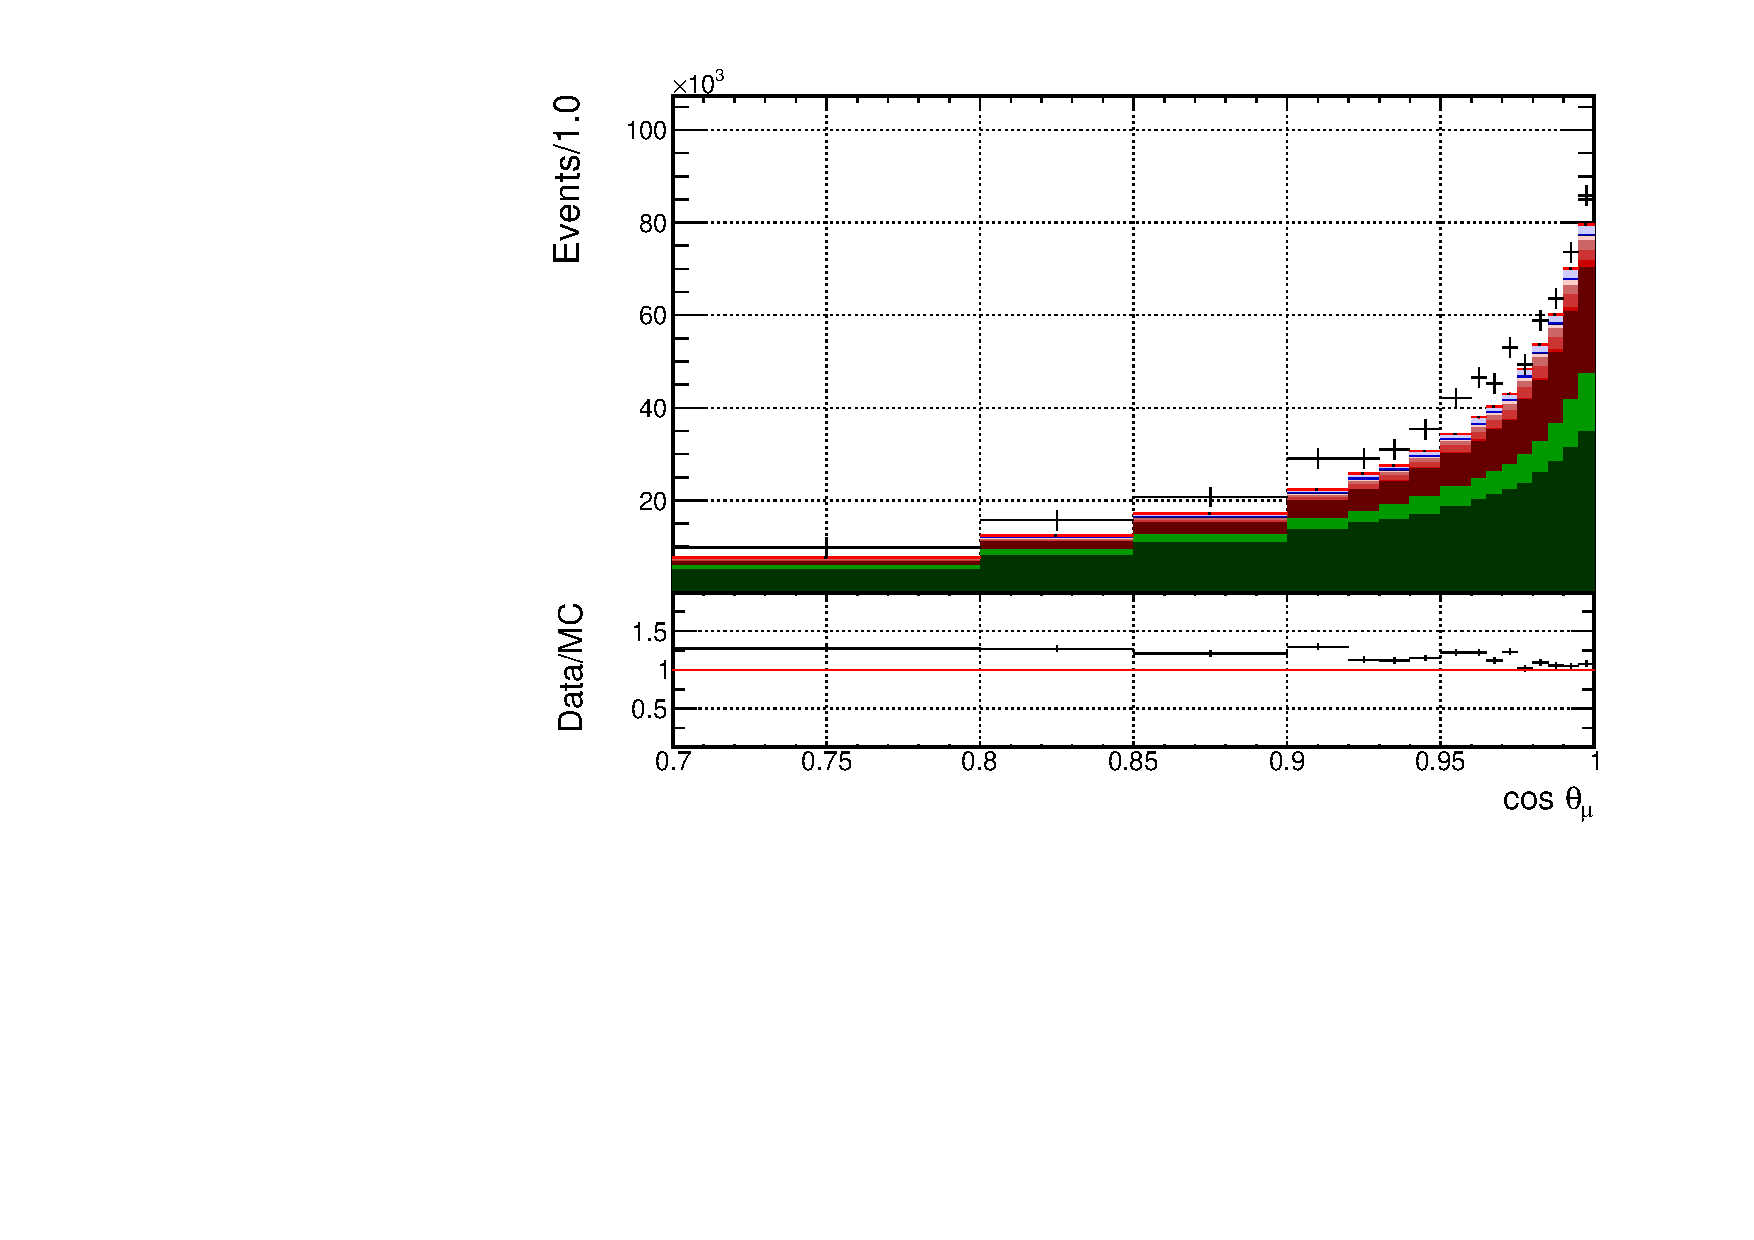
\includegraphics[width=\textwidth]{figs/FGD1_anti-numuCC_0pi_t}
  \caption{FGD1 RHC $\bar{\nu_{\mu}}$ 0$\pi$}
\end{subfigure}
\begin{subfigure}{0.49\textwidth}
  \centering
  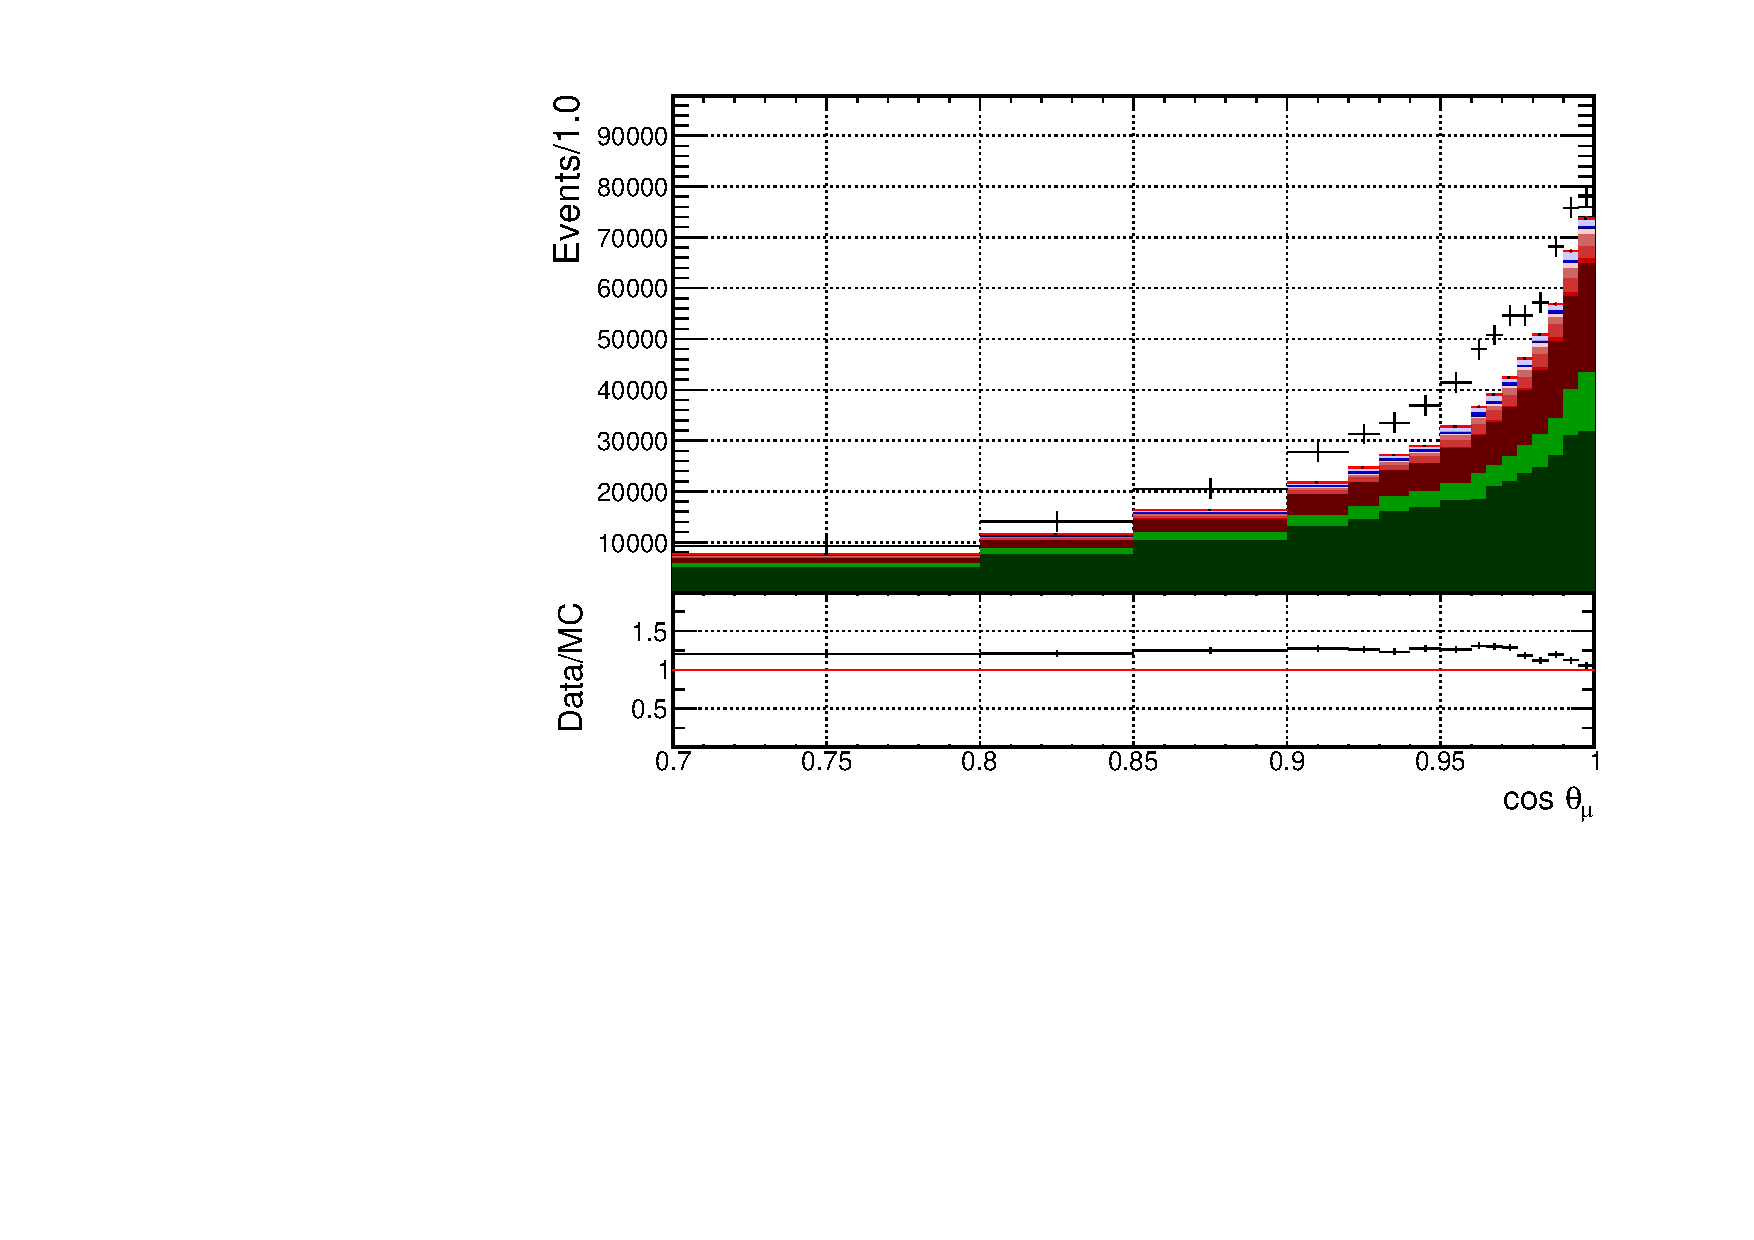
\includegraphics[width=\textwidth]{figs/FGD2_anti-numuCC_0pi_t}
  \caption{FGD2 RHC $\bar{\nu_{\mu}}$ 0$\pi$}
\end{subfigure}

\begin{subfigure}{0.49\textwidth}
  \centering
  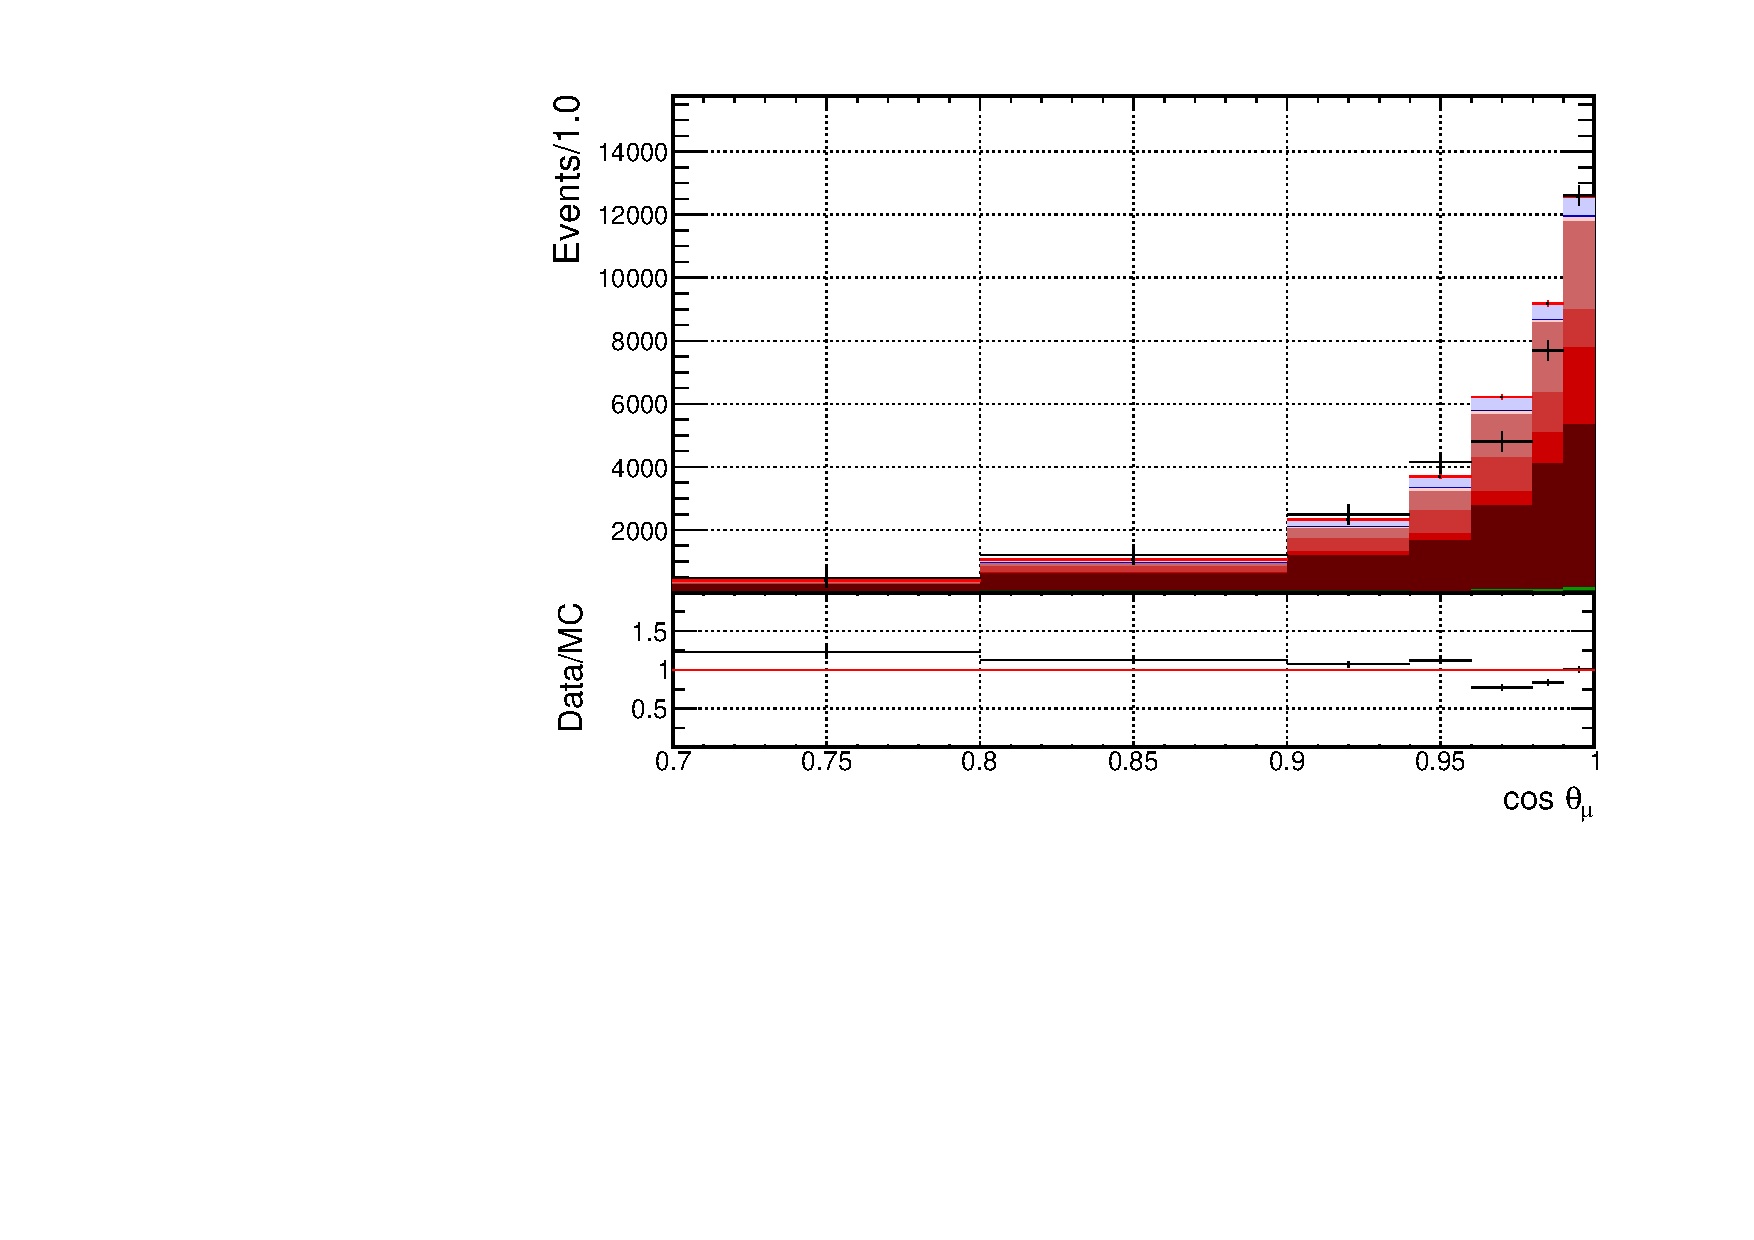
\includegraphics[width=\textwidth]{figs/FGD1_anti-numuCC_1pi_t}
  \caption{FGD1 RHC $\bar{\nu_{\mu}}$ 1$\pi$}
\end{subfigure}
\centering
\begin{subfigure}{0.49\textwidth}
  \centering
  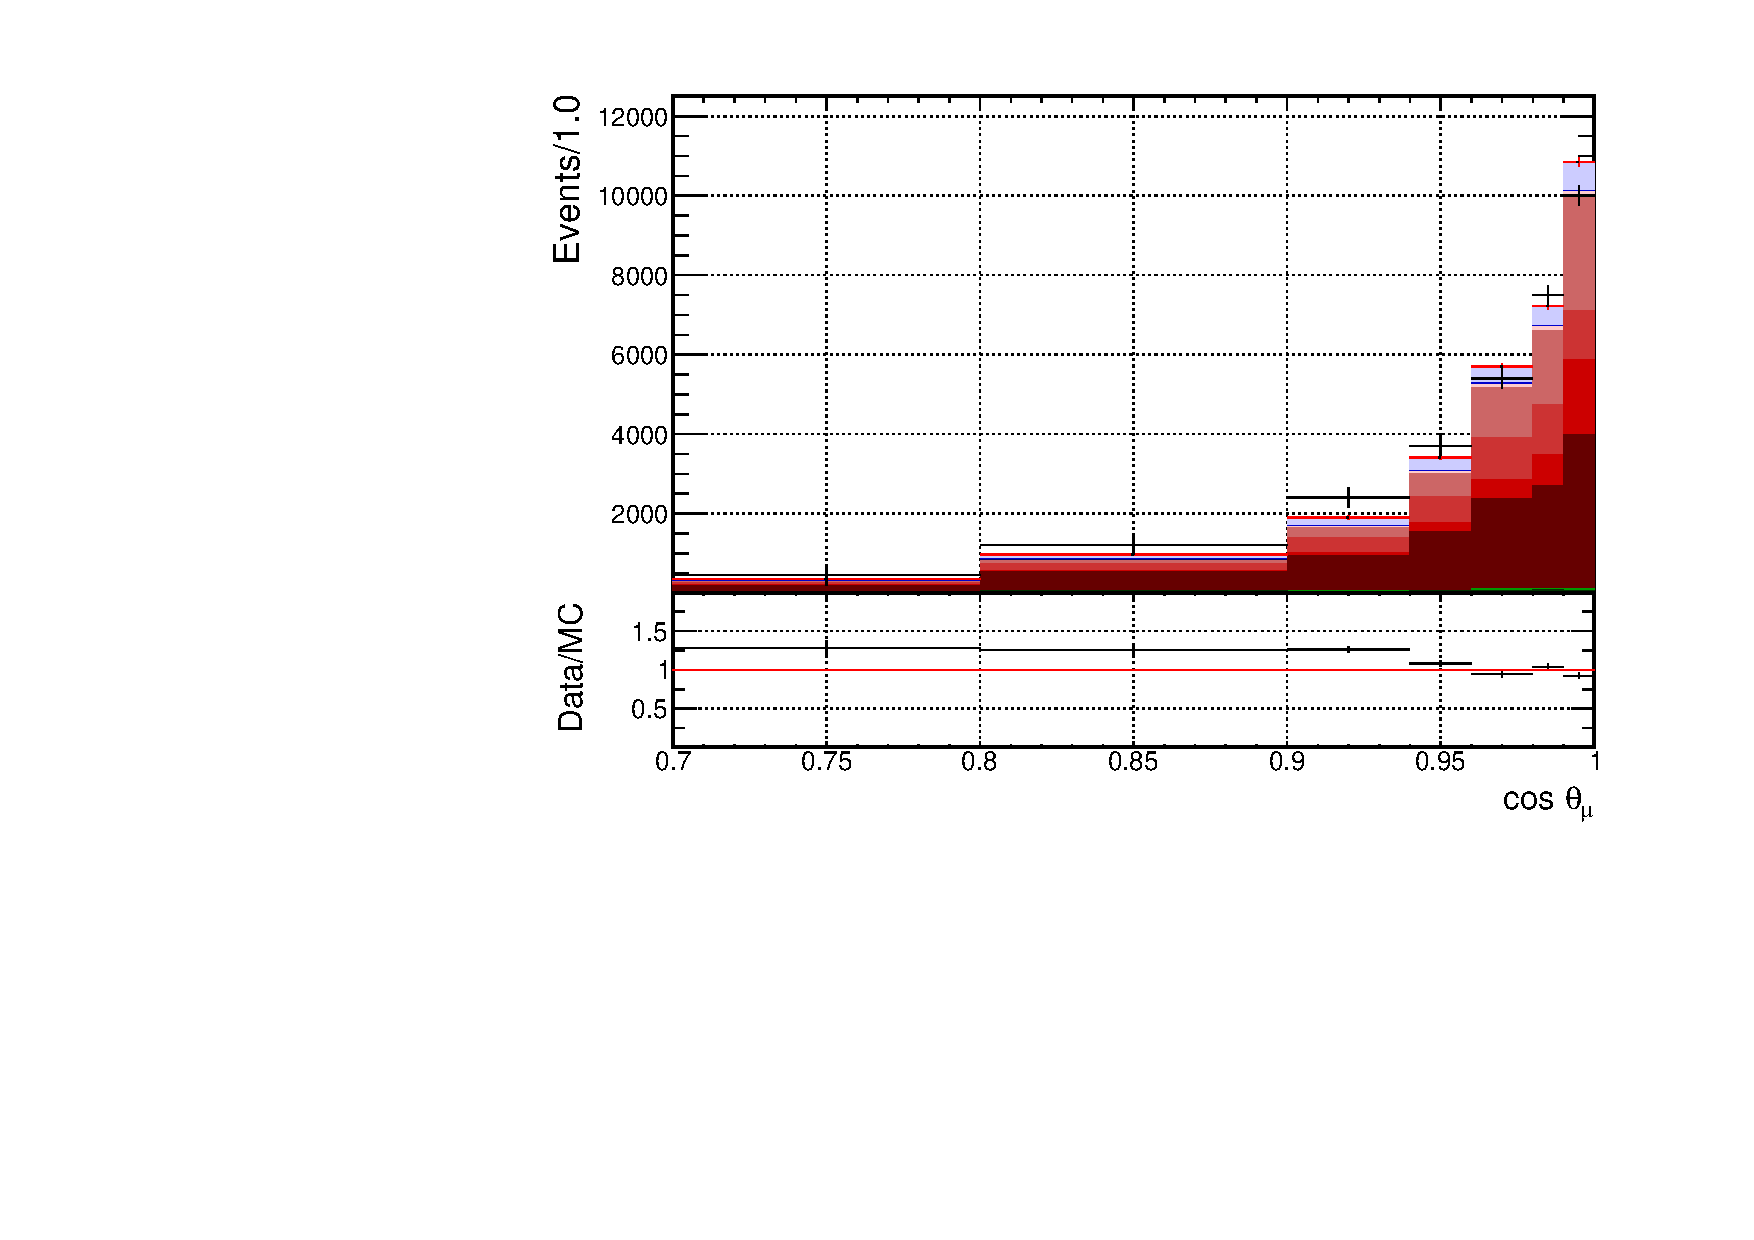
\includegraphics[width=\textwidth]{figs/FGD2_anti-numuCC_1pi_t}
  \caption{FGD2 RHC $\bar{\nu_{\mu}}$ 1$\pi$}
\end{subfigure}

\begin{subfigure}{0.49\textwidth}
  \centering
  \includegraphics[width=\textwidth]{figs/FGD1_anti-numuCC_other_t}
  \caption{FGD1 RHC $\bar{\nu_{\mu}}$ Other}
\end{subfigure}
\begin{subfigure}{0.49\textwidth}
  \centering
  \includegraphics[width=\textwidth]{figs/FGD2_anti-numuCC_other_t}
  \caption{FGD2 RHC $\bar{\nu_{\mu}}$ Other}
\end{subfigure}
\caption{$\cos\theta_{\mu}$ projections of data and nominal MC broken down by interaction mode for RHC \numub selections.}
\label{fig:tstack_rhc_numub}
\end{figure}

\begin{figure}[!h]
\centering
\begin{subfigure}{.24\textwidth}
  \centering
  \includegraphics[width=\linewidth, trim={5mm 60mm 30mm 0mm}, clip]{figs/legend}
\end{subfigure}
\begin{subfigure}{.24\textwidth}
  \centering
  \includegraphics[width=\linewidth, trim={5mm 0mm 30mm 80mm}, clip]{figs/legend}
\end{subfigure}
\begin{subfigure}{.24\textwidth}
  \centering
  \includegraphics[width=\linewidth, trim={5mm 60mm 30mm 0mm}, clip]{figs/legend2}
\end{subfigure}
\begin{subfigure}{.24\textwidth}
  \centering
  \includegraphics[width=\linewidth, trim={5mm 0mm 30mm 80mm}, clip]{figs/legend2}
\end{subfigure}

\begin{subfigure}{0.49\textwidth}
  \centering
  \includegraphics[width=\textwidth]{figs/FGD1_NuMuBkg_CC0pi_in_AntiNu_Mode_t}
  \caption{FGD1 RHC $\nu_{\mu}$ 0$\pi$}
\end{subfigure}
\begin{subfigure}{0.49\textwidth}
  \centering
  \includegraphics[width=\textwidth]{figs/FGD2_NuMuBkg_CC0pi_in_AntiNu_Mode_t}
  \caption{FGD2 RHC $\nu_{\mu}$ 0$\pi$}
\end{subfigure}

\begin{subfigure}{0.49\textwidth}
  \centering
  \includegraphics[width=\textwidth]{figs/FGD1_NuMuBkg_CC1pi_in_AntiNu_Mode_t}
  \caption{FGD1 RHC $\nu_{\mu}$ 1$\pi$}
\end{subfigure}
\begin{subfigure}{0.49\textwidth}
  \centering
  \includegraphics[width=\textwidth]{figs/FGD2_NuMuBkg_CC1pi_in_AntiNu_Mode_t}
  \caption{FGD2 RHC $\nu_{\mu}$ 1$\pi$}
\end{subfigure}

\begin{subfigure}{0.49\textwidth}
  \centering
  \includegraphics[width=\textwidth]{figs/FGD1_NuMuBkg_CCOther_in_AntiNu_Mode_t}
  \caption{FGD1 RHC $\nu_{\mu}$ Other}
\end{subfigure}
\begin{subfigure}{0.49\textwidth}
  \centering
  \includegraphics[width=\textwidth]{figs/FGD2_NuMuBkg_CCOther_in_AntiNu_Mode_t}
  \caption{FGD2 RHC $\nu_{\mu}$ Other}
\end{subfigure}
\caption{$\cos\theta_{\mu}$ projections of data and nominal MC broken down by interaction mode for RHC \numu selections.}
\label{fig:tstack_rhc_numu}
\end{figure}

\section{Log-likelihood Scans}\label{sec:llhscan}

As described in Section \ref{sec:extrac}, the marginalisation effects from extracting correlated and non-Gaussian parameters from the full posterior distribution can cause the fit to appear biased. A full Asimov fit alone, described in Section \ref{sec:asimov}, is therefore not a good method of validating the framework.

Log-likelihood scans are also run as part of the validations. The nominal MC is set as the data, and each systematic parameter is varied one at a time to 150 equally spaced points from -1$\sigma$ to +1$\sigma$. At each step, the MC is reweighted and the total likelihood from all contributions calculated. Only the diagonal terms of the covariance matrices are used for the penalty contribution, as otherwise varying one parameter alone could invoke significant penalties from correlations. The scans are therefore not a fully accurate measure of the sensitivity of the fit to constrain each systematic, but a useful validation of the framework.

After each scan, the parameter is reset, and the next parameter in question varied. The likelihood response is expected to be fairly Gaussian for each parameter, as the prior uncertainty is either Gaussian or flat, and most parameters are expected to have a symmetric effect on the number of events in individual bins. The minimum should be at the prior central value of the parameter, and the log-likelihood here should be 0, as at this point the reweighted MC is identical to the nominal MC. No variation of a single parameter should be able to produce a set of distributions more similar to the nominal MC than itself.

The log-likelihood scans for four selected interaction parameters are shown in Figure \ref{fig:llhxsec}. As expected, the test statistic minimises to 0 at the prior central value of each parameter. The penalty contribution to the log-likelihood dominates for the CC normalisation parameter, due to the prior uncertainty being so small. Conversely, the 2p2h $^{12}$C to $^{16}$O normalisation parameter has a weaker prior and therefore a larger contribution from the sample likelihood. The likelihood for the $0.05 < Q^2 < 0.10$ GeV$^2$ normalisation parameter is entirely dominated by the sample contribution, as the prior is flat. The CC DIS and mult-$\pi$ $\bar{\nu}$ normalisation parameter has more balanced contributions from both the sample and penalty likelihoods.

\begin{figure}
\centering
\begin{subfigure}{.49\textwidth}
  \centering
  \includegraphics[width=0.7\linewidth]{figs/llh/CC_norm_nu_llh.pdf}
  \caption{CC normalisation $\nu$}
\end{subfigure}
\begin{subfigure}{.49\textwidth}
  \centering
  \includegraphics[width=0.7\linewidth]{figs/llh/2p2h_normCtoO_llh.pdf}
  \caption{2p2h $^{12}$C  to $^{16}$O normalisation}
\end{subfigure}
\begin{subfigure}{.49\textwidth}
  \centering
  \includegraphics[width=0.7\linewidth]{figs/llh/Q2_norm_1_llh.pdf}
  \caption{$0.05 < Q^2 < 0.10$ normalisation}
\end{subfigure}
\begin{subfigure}{.49\textwidth}
  \centering
  \includegraphics[width=0.7\linewidth]{figs/llh/CC_DIS_MultPi_Norm_Nubar_llh.pdf}
  \caption{CC DIS and mult-$\pi$ normalisation}
\end{subfigure}
\caption{Log-likelihood scans for selected interaction parameters. CC norm. $\nu$ has a tight prior uncertainty that dominates the likelihood, whereas the low $Q^2$ normalisations have a flat prior so the sample is the only contribution. The 2p2h $^{12}$C to $^{16}$O and CC DIS and mult-$\pi$ normalisations have significant contributions from both the sample and prior uncertainty.}
\label{fig:llhxsec} 
\end{figure}

The log-likelihood scans for four selected flux parameters are shown in Figure \ref{fig:llhflux}. The test statistic again minimises to 0 at the prior central value of each parameter, as expected. These parameters all have tight prior uncertainties, and so the penalty terms dominate the likelihoods. For the SK flux parameters, there is no sample contribution to the likelihood. This is expected as the SK flux parameters should have no effect on the ND280 samples (apart from through the correlations with ND280 flux parameters, which are not included in these scans). 

\begin{figure}
\centering
\begin{subfigure}{.49\textwidth}
  \centering
  \includegraphics[width=0.7\linewidth]{figs/llh/b_5_llh.pdf}
  \caption{ND280 FHC $\nu_{\mu}$ 1-1.5 GeV}
\end{subfigure}
\begin{subfigure}{.49\textwidth}
  \centering
  \includegraphics[width=0.7\linewidth]{figs/llh/b_12_llh.pdf}
  \caption{ND280 FHC $\nu_{e}$ 0.5-0.7 GeV}
\end{subfigure}
\begin{subfigure}{.49\textwidth}
  \centering
  \includegraphics[width=0.7\linewidth]{figs/llh/b_36_llh.pdf}
  \caption{ND280 RHC $\nu_e$ 2.5-30 GeV}
\end{subfigure}
\begin{subfigure}{.49\textwidth}
  \centering
  \includegraphics[width=0.7\linewidth]{figs/llh/b_52_llh.pdf}
  \caption{SK RHC $\bar{\nu_{\mu}}$ 0.5-0.6 GeV}
\end{subfigure}
\caption{Log-likelihood scans for selected flux parameters. }
\label{fig:llhflux}
\end{figure}

The log-likelihood scans for four selected ND280 detector parameters are shown in Figure \ref{fig:llhdet}. As expected, the test statistics all minimise to 0 at the prior central value of each parameter. The prior dominates for all regions of $p_{\mu}$-cos$\theta_{\mu}$ in each sample. For the higher statistic regions (eg. FGD1 FHC $\nu_{\mu}$ CC 0$\pi$: 300-1000 MeV, 0.92-0.98), the overall constraint is larger than for the lower statistic regions, (eg. FGD1 FHC $\nu_{\mu}$ CC 1$\pi$: 5000-30000 MeV, -1.0-0.6). 

\begin{figure}
\centering
\begin{subfigure}{.49\textwidth}
  \centering
  \includegraphics[width=0.7\linewidth]{figs/llh/ndd_13_llh.pdf}
  \caption{FGD1 FHC $\nu_{\mu}$ CC 0$\pi$: 300-1000 MeV, 0.92-0.98}
\end{subfigure}
\begin{subfigure}{.49\textwidth}
  \centering
  \includegraphics[width=0.7\linewidth]{figs/llh/ndd_136_llh.pdf}
  \caption{FGD1 FHC $\nu_{\mu}$ CC 1$\pi$: 5000-30000 MeV, -1.0-0.6}
\end{subfigure}
\begin{subfigure}{.49\textwidth}
  \centering
  \includegraphics[width=0.7\linewidth]{figs/llh/ndd_541_llh.pdf}
  \caption{FGD2 RHC $\bar{\nu_{\mu}}$ CC Other: 800-30000 MeV, 0.97-1.0}
\end{subfigure}
\begin{subfigure}{.49\textwidth}
  \centering
  \includegraphics[width=0.7\linewidth]{figs/llh/ndd_556_llh.pdf}
  \caption{FGD1 RHC $\nu_{\mu}$ CC Other: 600-30000 MeV, -1.0-0.7}
\end{subfigure}
\caption{Log-likelihood scans for selected ND280 detector parameters.}
\label{fig:llhdet}
\end{figure}

\section{Parameter Variations}\label{sec:sigvar}

As a further validation of the fitting framework and models, the parameters are again each set to $\pm1\sigma$, one by one, while all others are held at nominal. Instead of the change in likelihood, here the effect on the event distributions in $p_{\mu}$-cos$\theta_{\mu}$ is inspected. 

One varied interaction parameter for each sample is shown in Figure \ref{fig:sigvars}. The combinations of parameter and sample were selected such that the parameter controls interactions targeted by the sample. The parameter is therefore expected to have a significant and well-understood impact on the shown sample. The selection of parameter and sample was also made such that no parameters are shown more than once. The parameter in question is set to $+1\sigma$ above its nominal value, and the ratio of the reweighted MC to the nominal MC is taken.

\begin{figure}
\centering
\begin{subfigure}{.32\textwidth}
  \centering
  \includegraphics[width=0.85\linewidth]{figs/sig/FGD1_numuCC_0pi_2p2h_norm_nu_+1sig.pdf}
  \caption{FGD1 FHC $\nu_{\mu}$ 0$\pi$: 2p2h Norm. $\nu$ += $1\sigma$}
  \label{fig:sigvar_FGD1_numuCC_0pi}
\end{subfigure}
\begin{subfigure}{.32\textwidth}
  \centering
  \includegraphics[width=0.85\linewidth]{figs/sig/FGD1_numuCC_1pi_FEFQEH_+1sig.pdf}
  \caption{FGD1 FHC $\nu_{\mu}$ 1$\pi$: $\pi$ FSI QE High E += $1\sigma$}
  \label{fig:sigvar_FGD1_numuCC_1pi}
\end{subfigure}
\begin{subfigure}{.32\textwidth}
  \centering
  \includegraphics[width=0.85\linewidth]{figs/sig/FGD1_numuCC_other_CC_AGKY_Mult_+1sig.pdf}
  \caption{FGD1 FHC $\nu_{\mu}$ Other: CC AGKY Mult. += $1\sigma$}
  \label{fig:sigvar_FGD1_numuCC_other}
\end{subfigure}
\centering
\begin{subfigure}{.32\textwidth}
  \centering
  \includegraphics[width=0.85\linewidth]{figs/sig/FGD2_numuCC_0pi_Q2_norm_7_+1sig.pdf}
  \caption{FGD2 FHC $\nu_{\mu}$ 0$\pi$: $Q^2 > 1.0$ GeV$^2$ += $1\sigma$}
  \label{fig:sigvar_FGD2_numuCC_0pi}
\end{subfigure}
\begin{subfigure}{.32\textwidth}
  \centering
  \includegraphics[width=0.85\linewidth]{figs/sig/FGD2_numuCC_1pi_CA5_+1sig.pdf}
  \caption{FGD2 FHC $\nu_{\mu}$ 1$\pi$: CA5 += $1\sigma$}
  \label{fig:sigvar_FGD2_numuCC_1pi}
\end{subfigure}
\begin{subfigure}{.32\textwidth}
  \centering
  \includegraphics[width=0.85\linewidth]{figs/sig/FGD2_numuCC_other_CC_DIS_MultPi_Norm_Nu_+1sig.pdf}
  \caption{FGD2 FHC $\nu_{\mu}$ Other: DIS/mult $\pi$ Norm. $\nu$ += $1\sigma$}
  \label{fig:sigvar_FGD2_numuCC_other}
\end{subfigure}
\centering
\begin{subfigure}{.32\textwidth}
  \centering
  \includegraphics[width=0.85\linewidth]{figs/sig/FGD1_anti-numuCC_0pi_MAQE_+1sig.pdf}
  \caption{FGD1 RHC $\bar{\nu_{\mu}}$ 0$\pi$: MAQE += $1\sigma$}
  \label{fig:sigvar_FGD1_anti-numuCC_0pi}
\end{subfigure}
\begin{subfigure}{.32\textwidth}
  \centering
  \includegraphics[width=0.85\linewidth]{figs/sig/FGD1_anti-numuCC_1pi_MARES_+1sig.pdf}
  \caption{FGD1 RHC $\bar{\nu_{\mu}}$ 1$\pi$: $M^{RES}_{A}$ += $1\sigma$}
  \label{fig:sigvar_FGD1_anti-numuCC_1pi}
\end{subfigure}
\begin{subfigure}{.32\textwidth}
  \centering
  \includegraphics[width=0.85\linewidth]{figs/sig/FGD1_anti-numuCC_other_CC_BY_DIS_+1sig.pdf}
  \caption{FGD1 RHC $\bar{\nu_{\mu}}$ Other: BY DIS += $1\sigma$}
  \label{fig:sigvar_FGD1_anti-numuCC_other}
\end{subfigure}
\centering
\begin{subfigure}{.32\textwidth}
  \centering
  \includegraphics[width=0.85\linewidth]{figs/sig/FGD2_anti-numuCC_0pi_EB_dial_O_nubar_+1sig.pdf}
  \caption{FGD2 RHC $\bar{\nu_{\mu}}$ 0$\pi$: $E_{b}$ $^{16}$O $\bar{\nu}$ += $1\sigma$}
  \label{fig:sigvar_FGD2_anti-numuCC_0pi}
\end{subfigure}
\begin{subfigure}{.32\textwidth}
  \centering
  \includegraphics[width=0.85\linewidth]{figs/sig/FGD2_anti-numuCC_1pi_ISO_BKG_+1sig.pdf}
  \caption{FGD2 RHC $\bar{\nu_{\mu}}$ 1$\pi$: $I_{1/2}$ += $1\sigma$}
  \label{fig:sigvar_FGD2_anti-numuCC_1pi}
\end{subfigure}
\begin{subfigure}{.32\textwidth}
  \centering
  \includegraphics[width=0.85\linewidth]{figs/sig/FGD2_anti-numuCC_other_CC_DIS_MultPi_Norm_Nubar_+1sig.pdf}
  \caption{FGD2 RHC $\bar{\nu_{\mu}}$ Other: DIS/mult-$\pi$ Norm. $\bar{\nu}$ += $1\sigma$}
  \label{fig:sigvar_FGD2_anti-numuCC_other}
\end{subfigure}
\begin{subfigure}{.32\textwidth}
  \centering
  \includegraphics[width=0.85\linewidth]{figs/sig/FGD1_NuMuBkg_CC0pi_in_AntiNu_Mode_2p2h_shape_C_+1sig.pdf}
  \caption{FGD1 RHC $\nu_{\mu}$ 0$\pi$: 2p2h Shape $^{12}$C += $1\sigma$}
  \label{fig:sigvar_FGD1_NuMuBkg_CC0pi_in_AntiNu_Mode}
\end{subfigure}
\begin{subfigure}{.32\textwidth}
  \centering
  \includegraphics[width=0.85\linewidth]{figs/sig/FGD1_NuMuBkg_CC1pi_in_AntiNu_Mode_CC_Coh_C_+1sig.pdf}
  \caption{FGD1 RHC $\nu_{\mu}$ 1$\pi$: CC Coh $^{12}$C += $1\sigma$}
  \label{fig:sigvar_FGD1_NuMuBkg_CC1pi_in_AntiNu_Mode}
\end{subfigure}
\begin{subfigure}{.32\textwidth}
  \centering
  \includegraphics[width=0.85\linewidth]{figs/sig/FGD1_NuMuBkg_CCOther_in_AntiNu_Mode_CC_Misc_+1sig.pdf}
  \caption{FGD1 RHC $\nu_{\mu}$ Other: CC Misc. += $1\sigma$}
  \label{fig:sigvar_FGD1_NuMuBkg_CCOther_in_AntiNu_Mode}
\end{subfigure}
\begin{subfigure}{.32\textwidth}
  \centering
  \includegraphics[width=0.85\linewidth]{figs/sig/FGD2_NuMuBkg_CC0pi_in_AntiNu_Mode_Q2_norm_0_+1sig.pdf}
  \caption{FGD2 RHC $\nu_{\mu}$ 0$\pi$: $0.00 < Q^2 < 0.05$ GeV$^2$ += $1\sigma$}
  \label{fig:sigvar_FGD2_NuMuBkg_CC0pi_in_AntiNu_Mode}
\end{subfigure}
\begin{subfigure}{.32\textwidth}
  \centering
  \includegraphics[width=0.85\linewidth]{figs/sig/FGD2_NuMuBkg_CC1pi_in_AntiNu_Mode_FEFABS_+1sig.pdf}
  \caption{FGD2 RHC $\nu_{\mu}$ 1$\pi$: $\pi$ FSI Abs += $1\sigma$}
  \label{fig:sigvar_FGD2_NuMuBkg_CC1pi_in_AntiNu_Mode}
\end{subfigure}
\begin{subfigure}{.32\textwidth}
  \centering
  \includegraphics[width=0.85\linewidth]{figs/sig/FGD2_NuMuBkg_CCOther_in_AntiNu_Mode_CC_BY_MPi_+1sig.pdf}
  \caption{FGD2 RHC $\nu_{\mu}$ Other: BY mult-$\pi$ += $1\sigma$}
  \label{fig:sigvar_FGD2_NuMuBkg_CCOther_in_AntiNu_Mode}
\end{subfigure}
\caption{Ratio of each sample to nominal with one parameter set to $+1\sigma$. The selected parameters shown all affect interactions which the sample they are shown for target.}
\label{fig:sigvars}
\end{figure}

The 2p2h $\nu$ normalisation, $Q^2$ normalisations, and $M^{QE}_A$ parameters all have a $Q^2$ dependence in the response of event distributions when set to $+1\sigma$. $M^{QE}_A$ and $Q^{2}>1.0$ GeV$^2$ have a larger effect at high Q$^2$, while the $0.00<Q^{2}<0.05$ GeV$^2$ controls the lower Q$^2$ region, as would be expected.

The $\pi$ FSI, and 2p2h shape $^{12}$C parameters reduce the number of events in the shown samples, despite being set higher than nominal. This is because they are not normalisation parameters, and so the weight applied can be lower for a higher parameter value. The AGKY mult-$\pi$, $C^{A}_{5}$, $M^{RES}_{A}$, BY DIS, BY mult-$\pi$, and $I_{1/2}$ uncertainties are all shape parameters which cause an increase in events in the samples shown when set to $+1\sigma$. The $E_{b}$ $^{16}$O $\bar{\nu}$ parameter causes an increase in events at low momentum, and decrease at higher momentum, as the events are directly shifted and not just reweighted.

The DIS normalisations, CC coh. $^{16}$O, and CC misc. normalisations all increase events at high angle when set to $+1\sigma$. The DIS normalisations effect higher momentum events, as would be expected as DIS interactions tend to involve higher energies. The CC misc. parameter has a large impact despite only affecting a small number of events, because of its large uncertainty. When it is set to $+1\sigma$ it therefore is significantly higher than at nominal.

All the variations are causing changes to the event distributions in the regions each parameter would be expected to. The total number of events in each sample at each variation was compared with the other near detector fitting group to verify that each parameter is behaving in the same way in each framework. Good agreement was found for all parameters, for all samples.

\section{Asimov Fit}\label{sec:asimov}

The Asimov dataset\footnote{Named after the Isaac Asimov short story, \textit{Franchise} \cite{asmv}, in which an individual is chosen as the sole voter as their views represent those of the whole population.} is defined as the MC prediction with all systematic parameters set to their nominal values \cite{Cowan_2011}. For an Asimov fit, the nominal MC prediction is set to be the `data', and is then fitted to itself. This is completely unphysical, as there can be a non-integer number of `data' events, but means there are no statistical fluctuations in the dataset, and the expected result of the fit is known. Therefore any deviations from the expected result indicate problems with the fitter. The results can also be used to obtain the maximum sensitivity of the fit. The constraint on each parameter shows the reduction in systematic uncertainties that would be achieved if the models perfectly described the true data.

The results of the Asimov fit for the flux parameters are shown in Figure \ref{fig:asmvfluxSK}. As described in Section \ref{sec:stats}, the fit does not find a single best-fit set of parameters, but single parameter values are extracted from the posterior distribution by marginalising over all but one parameter, one by one. Marginalisation effects cause the postfit parameter values to not exactly equal the nominal inputs, but the discrepancies are small. The flux parameters with the largest discrepancies are those that apply to rarer events at ND280, such as for high energies, and so are constrained mostly by the prior uncertainty only. The constraint on the SK flux parameters comes entirely from the correlation with the ND280 flux parameters, and so the postfit values have the same behaviour.

\begin{figure}
\centering
\begin{subfigure}{0.8\textwidth}
  \centering
  \includegraphics[width=0.24\linewidth]{figs/asmv_leg}
\end{subfigure}
\begin{subfigure}{0.45\textwidth}
  \centering
  \includegraphics[width=0.75\linewidth]{figs/asmvflux0}
  \caption{ND FHC $\nu_{\mu}$}
\end{subfigure}
\begin{subfigure}{0.45\textwidth}
  \centering
  \includegraphics[width=0.75\linewidth]{figs/asmvflux1}
  \caption{ND FHC $\bar{\nu_{\mu}}$}
\end{subfigure}
\begin{subfigure}{0.45\textwidth}
  \centering
  \includegraphics[width=0.75\linewidth]{figs/asmvflux2}
  \caption{ND FHC $\nu_e$}
\end{subfigure}
\begin{subfigure}{0.45\textwidth}
  \centering
  \includegraphics[width=0.75\linewidth]{figs/asmvflux3}
  \caption{ND FHC $\bar{\nu_{e}}$}
\end{subfigure}
\begin{subfigure}{0.45\textwidth}
  \centering
  \includegraphics[width=0.75\linewidth]{figs/asmvflux4}
  \caption{ND RHC $\nu_{\mu}$}
\end{subfigure}
\begin{subfigure}{0.45\textwidth}
  \centering
  \includegraphics[width=0.75\linewidth]{figs/asmvflux5}
  \caption{ND RHC $\bar{\nu_{\mu}}$}
\end{subfigure}
\begin{subfigure}{0.45\textwidth}
  \centering
  \includegraphics[width=0.75\linewidth]{figs/asmvflux6}
  \caption{ND RHC $\nu_{e}$}
\end{subfigure}
\begin{subfigure}{0.45\textwidth}
  \centering
  \includegraphics[width=0.75\linewidth]{figs/asmvflux7}
  \caption{ND RHC $\bar{\nu_e}$}
\end{subfigure}
\caption{ND280 flux parameters for the Asimov fit.}
\label{fig:asmvfluxND}
\end{figure}

\begin{figure}
\centering
\begin{subfigure}{0.8\textwidth}
  \centering
  \includegraphics[width=0.24\linewidth]{figs/asmv_leg}
\end{subfigure}
\begin{subfigure}{0.45\textwidth}
  \centering
  \includegraphics[width=0.75\linewidth]{figs/asmvflux8}
  \caption{SK FHC $\nu_{\mu}$}
\end{subfigure}
\begin{subfigure}{0.45\textwidth}
  \centering
  \includegraphics[width=0.75\linewidth]{figs/asmvflux9}
  \caption{SK FHC $\bar{\nu_{\mu}}$}
\end{subfigure}
\begin{subfigure}{0.45\textwidth}
  \centering
  \includegraphics[width=0.75\linewidth]{figs/asmvflux10}
  \caption{SK FHC $\nu_{e}$}
\end{subfigure}
\begin{subfigure}{0.45\textwidth}
  \centering
  \includegraphics[width=0.75\linewidth]{figs/asmvflux11}
  \caption{SK FHC $\bar{\nu_{e}}$}
\end{subfigure}
\begin{subfigure}{0.45\textwidth}
  \centering
  \includegraphics[width=0.75\linewidth]{figs/asmvflux12}
  \caption{SK RHC $\nu_{\mu}$}
\end{subfigure}
\begin{subfigure}{0.45\textwidth}
  \centering
  \includegraphics[width=0.75\linewidth]{figs/asmvflux13}
  \caption{SK RHC $\bar{\nu_{\mu}}$}
\end{subfigure}
\begin{subfigure}{0.45\textwidth}
  \centering
  \includegraphics[width=0.75\linewidth]{figs/asmvflux14}
  \caption{SK RHC $\nu_{e}$}
\end{subfigure}
\begin{subfigure}{0.45\textwidth}
  \centering
  \includegraphics[width=0.75\linewidth]{figs/asmvflux15}
  \caption{SK RHC $\bar{\nu_e}$}
\end{subfigure}
\caption{SK flux parameters for the Asimov fit.}
\label{fig:asmvfluxSK}
\end{figure}

The results for the interaction parameters are shown in Figure \ref{fig:asmvxsec}. All parameters stay close to their nominal values, as would be expected. There are several parameters which show small deviations, but these are again parameters which are not well constrained, such as NC 1$\gamma$, as there are few events of the relevant interaction mode at ND280. The 2p2h energy dependence and low $\pi$ momentum $I_{1/2}$ parameters are not fitted at the near detector so aren't shown here.

\begin{figure}
\centering
\begin{subfigure}{0.8\textwidth}
  \centering
  \includegraphics[width=0.25\linewidth]{figs/asmv_leg}
\end{subfigure}
\begin{subfigure}{0.49\textwidth}
  \centering
  \includegraphics[width=0.9\linewidth]{figs/asmvxsec1}
  \caption{CC0$\pi$}
\end{subfigure}
\begin{subfigure}{0.49\textwidth}
  \centering
  \includegraphics[width=0.9\linewidth]{figs/asmvxsec2}
  \caption{$Q^2$ and $E_b$}
\end{subfigure}
\begin{subfigure}{0.49\textwidth}
  \centering
  \includegraphics[width=0.9\linewidth]{figs/asmvxsec3}
  \caption{CC1$\pi$, $\nu_e$, CC DIS, CC mult-$\pi$ and CC Coh.}
\end{subfigure}
\begin{subfigure}{0.49\textwidth}
  \centering
  \includegraphics[width=0.9\linewidth]{figs/asmvxsec4}
  \caption{NC}
\end{subfigure}
\begin{subfigure}{0.49\textwidth}
  \centering
  \includegraphics[width=0.9\linewidth]{figs/asmvxsec4}
  \caption{$\pi$ FSI}
\end{subfigure}
\caption{Interaction parameters for the Asimov fit.}
\label{fig:asmvxsec}
\end{figure}

The postfit correlation matrix for flux and interaction parameters is shown in Figure \ref{fig:asmvpostfitcov}. There are strong correlations between uncertainties which control interactions with similar topologies, such as the $M^{QE}_A$, 2p2h, and $Q^2$ parameters. These all affect different regions of $Q^2$, but also all correlate with the flux parameters, causing them to correlate with other. The CC coherent parameters correlate with each other, and the CC 1$\pi$ parameters. There are strong internal correlations for the $E_b$, $\pi$ FSI and single $\pi$ production parameters. There are also slight correlations between CCQE and CC 1$\pi$ parameters, due to the contamination of CC $1\pi$ events in the CC 0$\pi$ samples. The flux parameters have strong internal correlations from their priors, and are anti-correlated with many interaction parameters, particularly normalisations.

\begin{figure}
\centering
\includegraphics*[width=0.9\textwidth,clip]{figs/Mach3AsmvCorr}
\caption{Asimov postfit correlation matrix for flux and interaction parameters.}\label{fig:asmvpostfitcov}
\end{figure}

\section{Data Fit}\label{sec:datafit}

\subsection{Prior Predictions}

Prior predictions are produced using a similar method to the posterior predictions described in Section \ref{sec:postpred}. However, instead of using draws from the Markov Chain, correlated throws of the fit parameters are made. For each of 2000 throws, the nominal MC is reweighted to the thrown parameter values. Each bin in each sample therefore has 2000 different number of events, from which the central value and uncertainty is used to build the prediction in the same way as for the posterior predictions. This method has the advantage of incorporating the prior uncertainties when inspecting how well the nominal model fits the data, which just looking at the nominal MC does not do. The prior prediction therefore gives a better gauge of how significant the discrepancies between the unfitted model and the data are. The nominal MC and prior prediction are not expected to be identical as they are constructed differently, the latter builds predictions from the prior and then averages whereas the former just takes the prior at the central value, but large discrepancies would be surprising.

The prior prediction can also be used to compare to the posterior predictive distributions, to show how the fit has changed not just the shape of the predictions, but also the uncertainties. The constraining of systematics by the fit is expected to reduce the uncertainties on the prediction.

The $p_{\mu}$ projections of the prior predictions for FHC sample are shown in Figure \ref{fig:priorpost_fhc_p}. The rest of the samples, and cos$\theta_{\mu}$ distributions are shown in Apprendix \ref{app:priorpred}.

As expected from comparisons of the nominal MC to data, the prior predictive distributions underestimate the data significantly, particularly in the peak region around $p_{\mu} \sim$600 MeV for the CC 0$\pi$ and CC Other samples. For the CC 1$\pi$ samples there are regions of significant overestimation. The levels of discrepancy are not concerning though, if the prior model perfectly described the data with small uncertainties the fit would not be needed. The prior predictions are compared to the posterior predictions in Table \ref{tab:predrates}.

\begin{figure}[!h]
\centering
\begin{subfigure}{.24\textwidth}
  \centering
  \includegraphics[width=\linewidth, clip]{figs/prioronly1dleg.pdf}
\end{subfigure}

\begin{subfigure}{0.49\textwidth}
  \centering
  \includegraphics[width=\textwidth]{figs/prioronly1D_p_FGD1_numuCC_0pi}
  \caption{FGD1 FHC $\nu_{\mu}$ 0$\pi$}
\end{subfigure}
\begin{subfigure}{0.49\textwidth}
  \centering
  \includegraphics[width=\textwidth]{figs/prioronly1D_p_FGD2_numuCC_0pi}
  \caption{FGD2 FHC $\nu_{\mu}$ 0$\pi$}
\end{subfigure}

\begin{subfigure}{0.49\textwidth}
  \centering
  \includegraphics[width=\textwidth]{figs/prioronly1D_p_FGD1_numuCC_1pi}
  \caption{FGD1 FHC $\nu_{\mu}$ 1$\pi$}
\end{subfigure}
\begin{subfigure}{0.49\textwidth}
  \centering
  \includegraphics[width=\textwidth]{figs/prioronly1D_p_FGD2_numuCC_1pi}
  \caption{FGD2 FHC $\nu_{\mu}$ 1$\pi$}
\end{subfigure}

\begin{subfigure}{0.49\textwidth}
  \centering
  \includegraphics[width=\textwidth]{figs/prioronly1D_p_FGD1_numuCC_other}
  \caption{FGD1 FHC $\nu_{\mu}$ Other}
\end{subfigure}
\begin{subfigure}{0.49\textwidth}
  \centering
  \includegraphics[width=\textwidth]{figs/prioronly1D_p_FGD2_numuCC_other}
  \caption{FGD2 FHC $\nu_{\mu}$ Other}
  \label{fig:priorpost_FGD2_numuCC_other}
\end{subfigure}
\caption{$p_{\mu}$ projections of the prior predictive distributions and data for FHC \numu selections.}
\label{fig:priorpost_fhc_p}
\end{figure}

\subsection{Fit Results}

The MC was then fitted to the real data. The postfit flux parameter values are shown in Figure \ref{fig:datfluxSK}. For FHC $\nu_{\mu}$ and $\nu_e$, there is a pull of $\sim$10$\%$ below 1 GeV. The pull decreases as the energy decreases, and falls below nominal at higher energies. A similarly high pull is seen for the FHC $\bar{\nu_{\mu}}$ parameters, but this is fairly constant in energy. For FHC $\bar{\nu_e}$ and RHC $\nu_e$, the pull is $\sim10\%$ for the high energy parameter, but the low energy parameter is close to its nominal value.

The RHC $nu_{\mu}$ parameters are also pulled significantly upwards, to $\sim$15$\%$. The pull oscillates around $\sim$10$\%$ as energy increases. The RHC $\bar{\nu_{\mu}}$ and $\bar{\nu_{e}}$ parameters are pulled to $\sim$10$\%$, but are closer to nominal above 2.5 GeV. Similar behaviour is seen for the ND280 and SK parameters, as would be expected due to their prefit correlations.

Although many of the flux parameters are pulled significantly away from their prior central values, and beyond the prefit $\pm1\sigma$ range, these results do not represent a strong bias in the fit. As the flux parameters are so strongly correlated, a pull in one translates to many of them moving. The flux penalty contribution to the log-likelihood at each step in the Markov Chain is shown in Figure \ref{fig:llh_fluxdat}. The stationary distribution is at -LLH$\approx$50, which for 100 flux parameters corresponds to $\sim1$ unit of $\chi^2$ per degree of freedom.

\begin{figure}
\centering
\begin{subfigure}{0.8\textwidth}
  \centering
  \includegraphics[width=0.24\linewidth]{figs/dat_leg}
\end{subfigure}
\begin{subfigure}{0.45\textwidth}
  \centering
  \includegraphics[width=0.75\linewidth]{figs/datflux0}
  \caption{ND FHC $\nu_{\mu}$}
\end{subfigure}
\begin{subfigure}{0.45\textwidth}
  \centering
  \includegraphics[width=0.75\linewidth]{figs/datflux1}
  \caption{ND FHC $\bar{\nu_{\mu}}$}
\end{subfigure}
\begin{subfigure}{0.45\textwidth}
  \centering
  \includegraphics[width=0.75\linewidth]{figs/datflux2}
  \caption{ND FHC $\nu_{e}$}
\end{subfigure}
\begin{subfigure}{0.45\textwidth}
  \centering
  \includegraphics[width=0.75\linewidth]{figs/datflux3}
  \caption{ND FHC $\bar{\nu_{e}}$}
\end{subfigure}
\begin{subfigure}{0.45\textwidth}
  \centering
  \includegraphics[width=0.75\linewidth]{figs/datflux4}
  \caption{ND RHC $\nu_{\mu}$}
\end{subfigure}
\begin{subfigure}{0.45\textwidth}
  \centering
  \includegraphics[width=0.75\linewidth]{figs/datflux5}
  \caption{ND RHC $\bar{\nu_{\mu}}$}
\end{subfigure}
\begin{subfigure}{0.45\textwidth}
  \centering
  \includegraphics[width=0.75\linewidth]{figs/datflux6}
  \caption{ND RHC $\nu_{e}$}
\end{subfigure}
\begin{subfigure}{0.45\textwidth}
  \centering
  \includegraphics[width=0.75\linewidth]{figs/datflux7}
  \caption{ND RHC $\bar{\nu_e}$}
\end{subfigure}
\caption{ND280 flux parameters for the data fit.}
\label{fig:datfluxND}
\end{figure}

\begin{figure}
\centering
\begin{subfigure}{0.8\textwidth}
  \centering
  \includegraphics[width=0.24\linewidth]{figs/dat_leg}
\end{subfigure}
\begin{subfigure}{0.45\textwidth}
  \centering
  \includegraphics[width=0.75\linewidth]{figs/datflux8}
  \caption{SK FHC $\nu_{\mu}$}
\end{subfigure}
\begin{subfigure}{0.45\textwidth}
  \centering
  \includegraphics[width=0.75\linewidth]{figs/datflux9}
  \caption{SK FHC $\bar{\nu_{\mu}}$}
\end{subfigure}
\begin{subfigure}{0.45\textwidth}
  \centering
  \includegraphics[width=0.75\linewidth]{figs/datflux10}
  \caption{SK FHC $\nu_{e}$}
\end{subfigure}
\begin{subfigure}{0.45\textwidth}
  \centering
  \includegraphics[width=0.75\linewidth]{figs/datflux11}
  \caption{SK FHC $\bar{\nu_{e}}$}
\end{subfigure}
\begin{subfigure}{0.45\textwidth}
  \centering
  \includegraphics[width=0.75\linewidth]{figs/datflux12}
  \caption{SK RHC $\nu_{\mu}$}
\end{subfigure}
\begin{subfigure}{0.45\textwidth}
  \centering
  \includegraphics[width=0.75\linewidth]{figs/datflux13}
  \caption{SK RHC $\bar{\nu_{\mu}}$}
\end{subfigure}
\begin{subfigure}{0.45\textwidth}
  \centering
  \includegraphics[width=0.75\linewidth]{figs/datflux14}
  \caption{SK RHC $\nu_{e}$}
\end{subfigure}
\begin{subfigure}{0.45\textwidth}
  \centering
  \includegraphics[width=0.75\linewidth]{figs/datflux15}
  \caption{SK RHC $\bar{\nu_e}$}
\end{subfigure}
\caption{SK flux parameters for the data fit.}
\label{fig:datfluxSK}
\end{figure}

\begin{figure}
\centering
\includegraphics*[width=0.7\textwidth,clip]{figs/llh_fluxdat}
\caption{Flux penalty contribution to the log-likelihood at each step in the data fit.}\label{fig:llh_fluxdat}
\end{figure}

The interaction parameters are shown in Figure \ref{fig:datxsec}. The $M^{QE}_A$ parameter is pulled above its prior central value to much closer to the nominal generated value (corresponding to 1.2 GeV$^2$). The 2p2h normalisations are all consistent with the nominal value within the postfit uncertainty. 2p2h shape $^{12}$C is the only 2p2h parameter pulled significantly away from nominal, to $\sim$1.7, favouring the Nieves model. This is not consistent with the 2p2h shape $^{16}$O parameter which is much closer to nominal.

The $Q^2$ normalisations all sit slightly above their prior central values, and the shape of the increase in parameter value with increasing $Q^2$ is similar to the priors. The $Q^2>1.0$ GeV$^2$ is the only $Q^2$ normalisation pulled significantly away from the prior.

The 1D distributions for the $E_b$ parameters are shown in Figure \ref{fig:Ebdatares}. Although the distributions are non-Gaussian, making it difficult to extract a single central value, the highest posterior densities, and arithmetic means are all within $1\sigma$ of the prior.

The $M_A^{RES}$ parameter is pulled down, beyond the prior uncertainty, while the other single $\pi$ production parameters are all consistent with their nominal values. This could suggest $M_A^{RES}$ is soaking up deficiencies in the single $\pi$ production model.

There is tension between the BY corrections, with the BY DIS parameter being pulled to the edge of its 100$\%$ prior uncertainty, and the BY mult-$\pi$ parameter staying at its nominal value. The CC misc. parameter is also pushed high, but has a large prior uncertainty. The other parameters targeting events in the CC Other samples are very consistent with their prior central values. 

The CC coherent, NC, and $\pi$ FSI parameters are all within $1\sigma$ of their nominal values, apart from NC Other ND280, which has very little constraint from the data due to low statistics. 

\begin{figure}
\centering
\begin{subfigure}{0.95\textwidth}
  \centering
  \includegraphics[width=0.25\linewidth]{figs/dat_leg}
\end{subfigure}
\begin{subfigure}{0.49\textwidth}
  \centering
  \includegraphics[width=0.9\linewidth]{figs/datxsec1}
  \caption{CC0$\pi$}
\end{subfigure}
\begin{subfigure}{0.49\textwidth}
  \centering
  \includegraphics[width=0.9\linewidth]{figs/datxsec2}
  \caption{$Q^2$ and $E_b$}
\end{subfigure}
\begin{subfigure}{0.49\textwidth}
  \centering
  \includegraphics[width=0.9\linewidth]{figs/datxsec3}
  \caption{CC1$\pi$, $\nu_e$, CC DIS, CC mult-$\pi$ and CC coh.}
\end{subfigure}
\begin{subfigure}{0.45\textwidth}
  \centering
  \includegraphics[width=0.9\linewidth]{figs/datxsec4}
  \caption{NC}
\end{subfigure}
\begin{subfigure}{0.49\textwidth}
  \centering
  \includegraphics[width=0.9\linewidth]{figs/datxsec5}
  \caption{$\pi$ FSI}
\end{subfigure}
\caption{Interaction parameters for the data fit.}
\label{fig:datxsec}
\end{figure}

\begin{figure}
\centering
\begin{subfigure}{.48\textwidth}
  \centering
  \includegraphics[width=0.73\linewidth]{figs/EB_dial_C_nuData}
  \caption{$E_{b}\nu$ C}
\end{subfigure}
\begin{subfigure}{.48\textwidth}
  \centering
  \includegraphics[width=0.73\linewidth]{figs/EB_dial_C_nubarData}
  \caption{$E_{b}\bar{\nu}$ C}
\end{subfigure} \\
\begin{subfigure}{.48\textwidth}
  \centering
  \includegraphics[width=0.73\linewidth]{figs/EB_dial_O_nuData}
  \caption{$E_{b}\nu$ O}
\end{subfigure}
\begin{subfigure}{.48\textwidth}
  \centering
  \includegraphics[width=0.73\linewidth]{figs/EB_dial_O_nubarData}
  \caption{$E_{b}\bar{\nu}$ O}
\end{subfigure}
\caption{Posterior distributions for the binding energy parameters from the data fit.}
\label{fig:Ebdatares}
\end{figure}

The post-data-fit covariance for the flux and interaction parameters is shown in Figure \ref{fig:datpostfitcov}. The overall trends are similar to what was seen for the Asimov fit in Figure \ref{fig:asmvpostfitcov}. The fluxes are strongly internally correlated, and anti-correlated with interaction normalisations. 

$M^{QE}_A$ correlates with the lowest $Q^2$ normalisation, which decreases as $Q^2$ increases, becoming a strong anti-correlation for the higher $Q^2$ parameters. This is expected as $M^{QE}_A$ affects higher $Q^2$ events, with the low $Q^2$ anti-correlation likely due to the mutual correlation with the flux parameters. $M^{QE}_A$ now also correlates highly with the $E_b$ parameters, having been anti-correlated with them in the Asimov fit.

The strength of the $E_b$ correlations and anti-correlations has increased since the Asimov fit. $E_b$ is correlated with the low energy, and anti-correlated with the high energy flux parameters. This is because as the $E_b$ parameters increase, the number of low lepton momentum events increases as events shifts to lower momentum. This can be compensated by low energy flux parameters decreasing, as lower energy neutrino events are likely to produce lower momentum leptons, and so the anti-correlations arise. The opposite is true for higher energies, causing positive correlations.

There are strong correlations between the 2p2h and CC 1$\pi$ parameters. This is likely due to final state interactions in which a $\pi$ is absorbed, causing CC 1$\pi$ events to be detected as CC 0$\pi$. The 2p2h shape parameters are more anti-correlated than for the Asimov fit. 2p2h shape $^{12}$C is still correlated with the $Q^2$ normalisations, with increasing strength at lower $Q^2$, whereas 2p2h shape $^{16}$O is now anti-correlated with them, with increasing strength at higher $Q^2$. Both 2p2h shape parameters are correlated with the fluxes, having been anti-correlated in the Asimov fit.

The $M_{A}^{RES}$ and $C_{A}^5$ parameters have a stronger anti-correlation with each other than in the data fit.

The $Q^2$ normalisations, DIS and mult-$\pi$, and $\pi$ FSI parameters all have internal correlations and anti-correlations, with a slight increase in strength compared to the Asimov fit. 

\begin{figure}
\centering
\includegraphics*[width=0.9\textwidth,clip]{figs/MaCh3DataCorr}
\caption{Data postfit correlation matrix for flux and interaction parameters.}\label{fig:datpostfitcov}
\end{figure}

\section{Posterior Predictions}\label{sec:respostpred}

Posterior predictions are produced using the method described in Section \ref{sec:postpred}. The $p_{\mu}$ and cos$\theta_{\mu}$ projections of the posterior predictions for each sample are shown in Figures \ref{fig:priorpost_fhc_p}-\ref{fig:priorpost_rhc_numu_t}, along with the prior predictions and data. There is significant improvement in the agreement with data for the posterior predictions compared to prior predictions. Particularly in the momentum peak around $p_{\mu}\sim$600 MeV, the prediction is closer to data. There are still regions of underestimation in the CC 0$\pi$ and CC Other samples, and overestimation in CC 1$\pi$ samples, but these are less strong than for the prior prediction. The error band is also reduced significantly for the posterior compared to the prior for all samples, showing how the constraint on systematic uncertainties from the fit has reduced the uncertainty in the prediction. 

This is confirmed by the reduction in -2LLH for the posterior prediction compared to for the prior prediction, shown in Table \ref{tab:predrates}. The uncertainties on the total event rate for all samples is also reduced significantly. The fractional errors in Table \ref{tab:prederr} show the overall ND280 event rate uncertainty has been reduced from $9.32\%$ $0.29\%$ by the fit.

\begin{figure}[!h]
\centering
\begin{subfigure}{.24\textwidth}
  \centering
  \includegraphics[width=\linewidth, clip]{figs/prior1dleg.pdf}
\end{subfigure}

\begin{subfigure}{0.49\textwidth}
  \centering
  \includegraphics[width=\textwidth]{figs/priorpred1D_p_FGD1_numuCC_0pi}
  \caption{FGD1 FHC $\nu_{\mu}$ 0$\pi$}
\end{subfigure}
\begin{subfigure}{0.49\textwidth}
  \centering
  \includegraphics[width=\textwidth]{figs/priorpred1D_p_FGD2_numuCC_0pi}
  \caption{FGD2 FHC $\nu_{\mu}$ 0$\pi$}
\end{subfigure}

\begin{subfigure}{0.49\textwidth}
  \centering
  \includegraphics[width=\textwidth]{figs/priorpred1D_p_FGD1_numuCC_1pi}
  \caption{FGD1 FHC $\nu_{\mu}$ 1$\pi$}
\end{subfigure}
\begin{subfigure}{0.49\textwidth}
  \centering
  \includegraphics[width=\textwidth]{figs/priorpred1D_p_FGD2_numuCC_1pi}
  \caption{FGD2 FHC $\nu_{\mu}$ 1$\pi$}
\end{subfigure}

\begin{subfigure}{0.49\textwidth}
  \centering
  \includegraphics[width=\textwidth]{figs/priorpred1D_p_FGD1_numuCC_other}
  \caption{FGD1 FHC $\nu_{\mu}$ Other}
\end{subfigure}
\begin{subfigure}{0.49\textwidth}
  \centering
  \includegraphics[width=\textwidth]{figs/priorpred1D_p_FGD2_numuCC_other}
  \caption{FGD2 FHC $\nu_{\mu}$ Other}
\end{subfigure}
\caption{$p_{\mu}$ projections of the prior and posterior predictive distributions and data for FHC \numu selections.}
\label{fig:priorpost_fhc_p}
\end{figure}

\begin{figure}[!h]
\centering
\begin{subfigure}{.24\textwidth}
  \centering
  \includegraphics[width=\linewidth, clip]{figs/prior1dleg.pdf}
\end{subfigure}

\begin{subfigure}{0.49\textwidth}
  \centering
  \includegraphics[width=\textwidth]{figs/priorpred1D_p_FGD1_anti-numuCC_0pi}
  \caption{FGD1 RHC $\bar{\nu_{\mu}}$ 0$\pi$}
\end{subfigure}
\begin{subfigure}{0.49\textwidth}
  \centering
  \includegraphics[width=\textwidth]{figs/priorpred1D_p_FGD2_anti-numuCC_0pi}
  \caption{FGD2 RHC $\bar{\nu_{\mu}}$ 0$\pi$}
\end{subfigure}

\begin{subfigure}{0.49\textwidth}
  \centering
  \includegraphics[width=\textwidth]{figs/priorpred1D_p_FGD1_anti-numuCC_1pi}
  \caption{FGD1 RHC $\bar{\nu_{\mu}}$ 1$\pi$}
\end{subfigure}
\centering
\begin{subfigure}{0.49\textwidth}
  \centering
  \includegraphics[width=\textwidth]{figs/priorpred1D_p_FGD2_anti-numuCC_1pi}
  \caption{FGD2 RHC $\bar{\nu_{\mu}}$ 1$\pi$}
\end{subfigure}

\begin{subfigure}{0.49\textwidth}
  \centering
  \includegraphics[width=\textwidth]{figs/priorpred1D_p_FGD1_anti-numuCC_other}
  \caption{FGD1 RHC $\bar{\nu_{\mu}}$ Other}
\end{subfigure}
\begin{subfigure}{0.49\textwidth}
  \centering
  \includegraphics[width=\textwidth]{figs/priorpred1D_p_FGD2_anti-numuCC_other}
  \caption{FGD2 RHC $\bar{\nu_{\mu}}$ Other}
\end{subfigure}
\caption{$p_{\mu}$ projections of the prior and posterior predictive distributions and data for RHC \numub selections.}
\label{fig:priorpost_rhc_numub_p}
\end{figure}

\begin{figure}[!h]
\centering
\begin{subfigure}{.24\textwidth}
  \centering
  \includegraphics[width=\linewidth, clip]{figs/prior1dleg.pdf}
\end{subfigure}

\begin{subfigure}{0.49\textwidth}
  \centering
  \includegraphics[width=\textwidth]{figs/priorpred1D_p_FGD1_NuMuBkg_CC0pi_in_AntiNu_Mode}
  \caption{FGD1 RHC $\nu_{\mu}$ 0$\pi$}
\end{subfigure}
\begin{subfigure}{0.49\textwidth}
  \centering
  \includegraphics[width=\textwidth]{figs/priorpred1D_p_FGD2_NuMuBkg_CC0pi_in_AntiNu_Mode}
  \caption{FGD2 RHC $\nu_{\mu}$ 0$\pi$}
\end{subfigure}

\begin{subfigure}{0.49\textwidth}
  \centering
  \includegraphics[width=\textwidth]{figs/priorpred1D_p_FGD1_NuMuBkg_CC1pi_in_AntiNu_Mode}
  \caption{FGD1 RHC $\nu_{\mu}$ 1$\pi$}
\end{subfigure}
\begin{subfigure}{0.49\textwidth}
  \centering
  \includegraphics[width=\textwidth]{figs/priorpred1D_p_FGD2_NuMuBkg_CC1pi_in_AntiNu_Mode}
  \caption{FGD2 RHC $\nu_{\mu}$ 1$\pi$}
\end{subfigure}

\begin{subfigure}{0.49\textwidth}
  \centering
  \includegraphics[width=\textwidth]{figs/priorpred1D_p_FGD1_NuMuBkg_CCOther_in_AntiNu_Mode}
  \caption{FGD1 RHC $\nu_{\mu}$ Other}
\end{subfigure}
\begin{subfigure}{0.49\textwidth}
  \centering
  \includegraphics[width=\textwidth]{figs/priorpred1D_p_FGD2_NuMuBkg_CCOther_in_AntiNu_Mode}
  \caption{FGD2 RHC $\nu_{\mu}$ Other}
\end{subfigure}
\caption{$p_{\mu}$ projections of the prior and posterior predictive distributions and data for RHC \numu selections.}
\label{fig:priorpost_rhc_numu_p}
\end{figure}

\begin{figure}[!h]
\centering
\begin{subfigure}{.24\textwidth}
  \centering
  \includegraphics[width=\linewidth, clip]{figs/prior1dleg.pdf}
\end{subfigure}

\begin{subfigure}{0.49\textwidth}
  \centering
  \includegraphics[width=\textwidth]{figs/priorpred1D_t_FGD1_numuCC_0pi}
  \caption{FGD1 FHC $\nu_{\mu}$ 0$\pi$}
\end{subfigure}
\begin{subfigure}{0.49\textwidth}
  \centering
  \includegraphics[width=\textwidth]{figs/priorpred1D_t_FGD2_numuCC_0pi}
  \caption{FGD2 FHC $\nu_{\mu}$ 0$\pi$}
\end{subfigure}

\begin{subfigure}{0.49\textwidth}
  \centering
  \includegraphics[width=\textwidth]{figs/priorpred1D_t_FGD1_numuCC_1pi}
  \caption{FGD1 FHC $\nu_{\mu}$ 1$\pi$}
\end{subfigure}
\begin{subfigure}{0.49\textwidth}
  \centering
  \includegraphics[width=\textwidth]{figs/priorpred1D_t_FGD2_numuCC_1pi}
  \caption{FGD2 FHC $\nu_{\mu}$ 1$\pi$}
\end{subfigure}

\begin{subfigure}{0.49\textwidth}
  \centering
  \includegraphics[width=\textwidth]{figs/priorpred1D_t_FGD1_numuCC_other}
  \caption{FGD1 FHC $\nu_{\mu}$ Other}
\end{subfigure}
\begin{subfigure}{0.49\textwidth}
  \centering
  \includegraphics[width=\textwidth]{figs/priorpred1D_t_FGD2_numuCC_other}
  \caption{FGD2 FHC $\nu_{\mu}$ Other}
\end{subfigure}
\caption{cos$\theta_{\mu}$ projections of the prior and posterior predictive distributions and data for FHC \numu selections.}
\label{fig:priorpost_fhc_t}
\end{figure}

\begin{figure}[!h]
\centering
\begin{subfigure}{.24\textwidth}
  \centering
  \includegraphics[width=\linewidth, clip]{figs/prior1dleg.pdf}
\end{subfigure}

\begin{subfigure}{0.49\textwidth}
  \centering
  \includegraphics[width=\textwidth]{figs/priorpred1D_t_FGD1_anti-numuCC_0pi}
  \caption{FGD1 RHC $\bar{\nu_{\mu}}$ 0$\pi$}
\end{subfigure}
\begin{subfigure}{0.49\textwidth}
  \centering
  \includegraphics[width=\textwidth]{figs/priorpred1D_t_FGD2_anti-numuCC_0pi}
  \caption{FGD2 RHC $\bar{\nu_{\mu}}$ 0$\pi$}
\end{subfigure}

\begin{subfigure}{0.49\textwidth}
  \centering
  \includegraphics[width=\textwidth]{figs/priorpred1D_t_FGD1_anti-numuCC_1pi}
  \caption{FGD1 RHC $\bar{\nu_{\mu}}$ 1$\pi$}
\end{subfigure}
\centering
\begin{subfigure}{0.49\textwidth}
  \centering
  \includegraphics[width=\textwidth]{figs/priorpred1D_t_FGD2_anti-numuCC_1pi}
  \caption{FGD2 RHC $\bar{\nu_{\mu}}$ 1$\pi$}
\end{subfigure}

\begin{subfigure}{0.49\textwidth}
  \centering
  \includegraphics[width=\textwidth]{figs/priorpred1D_t_FGD1_anti-numuCC_other}
  \caption{FGD1 RHC $\bar{\nu_{\mu}}$ Other}
\end{subfigure}
\begin{subfigure}{0.49\textwidth}
  \centering
  \includegraphics[width=\textwidth]{figs/priorpred1D_t_FGD2_anti-numuCC_other}
  \caption{FGD2 RHC $\bar{\nu_{\mu}}$ Other}
\end{subfigure}
\caption{cos$\theta_{\mu}$ projections of the prior and posterior predictive distributions and data for RHC \numub selections.}
\label{fig:priorpost_rhc_numub_t}
\end{figure}

\begin{figure}[!h]
\centering
\begin{subfigure}{.24\textwidth}
  \centering
  \includegraphics[width=\linewidth, clip]{figs/prior1dleg.pdf}
\end{subfigure}

\begin{subfigure}{0.49\textwidth}
  \centering
  \includegraphics[width=\textwidth]{figs/priorpred1D_t_FGD1_NuMuBkg_CC0pi_in_AntiNu_Mode}
  \caption{FGD1 RHC $\nu_{\mu}$ 0$\pi$}
\end{subfigure}
\begin{subfigure}{0.49\textwidth}
  \centering
  \includegraphics[width=\textwidth]{figs/priorpred1D_t_FGD2_NuMuBkg_CC0pi_in_AntiNu_Mode}
  \caption{FGD2 RHC $\nu_{\mu}$ 0$\pi$}
\end{subfigure}

\begin{subfigure}{0.49\textwidth}
  \centering
  \includegraphics[width=\textwidth]{figs/priorpred1D_t_FGD1_NuMuBkg_CC1pi_in_AntiNu_Mode}
  \caption{FGD1 RHC $\nu_{\mu}$ 1$\pi$}
\end{subfigure}
\begin{subfigure}{0.49\textwidth}
  \centering
  \includegraphics[width=\textwidth]{figs/priorpred1D_t_FGD2_NuMuBkg_CC1pi_in_AntiNu_Mode}
  \caption{FGD2 RHC $\nu_{\mu}$ 1$\pi$}
\end{subfigure}

\begin{subfigure}{0.49\textwidth}
  \centering
  \includegraphics[width=\textwidth]{figs/priorpred1D_t_FGD1_NuMuBkg_CCOther_in_AntiNu_Mode}
  \caption{FGD1 RHC $\nu_{\mu}$ Other}
\end{subfigure}
\begin{subfigure}{0.49\textwidth}
  \centering
  \includegraphics[width=\textwidth]{figs/priorpred1D_t_FGD2_NuMuBkg_CCOther_in_AntiNu_Mode}
  \caption{FGD2 RHC $\nu_{\mu}$ Other}
\end{subfigure}
\caption{cos$\theta_{\mu}$ projections of the prior and posterior predictive distributions and data for RHC \numu selections.}
\label{fig:priorpost_rhc_numu_t}
\end{figure}

\begin{center}
\begin{table}
\center
\begin{adjustbox}{max width=1.1\textwidth,center}
\begin{tabular}{S||
	  			r|
                r
                p{0.26cm}
                r
                |r
                p{0.26cm}
                r
                |r
                r}
\hline \hline
\multicolumn{1}{c||}{\textbf{Sample}} & \multicolumn{7}{c|}{\textbf{Event Rates}} & \multicolumn{2}{c}{\textbf{-2LLH$_{Sample}$}}\\
& \multicolumn{1}{c}{\textbf{Data}} & \multicolumn{3}{c}{\textbf{Prior}} & \multicolumn{3}{c|}{\textbf{Posterior}} & \multicolumn{1}{c}{\textbf{Prior}} & \multicolumn{1}{c}{\textbf{Posterior}}\\
\hline
\hline
\textbf{FGD1 FHC $\nu$ CC 0$\pi$} & 33443 & 28912.3 & $\pm$ & 3049.9 & 33375.4 & $\pm$ & 159.6 & 1699.87 & 877.22 \\ 
\textbf{FGD1 FHC $\nu$ CC 1$\pi$} & 7713 & 8691.5 & $\pm$ & 1013.2 & 7951.9 & $\pm$ & 64.2 & 436.38 & 293.07 \\
\textbf{FGD1 FHC $\nu$ CC Other} & 8026 & 7343.3 & $\pm$ & 1004.0 & 7917.0 & $\pm$ & 71.4 & 519.01 & 430.51\\ \hline
\textbf{FGD2 FHC $\nu$ CC 0$\pi$} & 33156 & 28461.0 & $\pm$ & 2998.9 & 33125.4 & $\pm$ & 157.6 & 1801.15 & 869.49 \\
\textbf{FGD2 FHC $\nu$ CC 1$\pi$} & 6281 & 6965.6 & $\pm$ & 791.5 & 6434.1 & $\pm$ & 56.8 & 411.05 & 315.77 \\
\textbf{FGD2 FHC $\nu$ CC Other} & 7700 & 6740.4 & $\pm$ & 893.0 & 7281.8 & $\pm$ & 64.8 & 541.39 & 404.94 \\ \hline
\textbf{FGD1 RHC $\bar{\nu}$ CC 0$\pi$} & 8388 & 7665.0 & $\pm$ & 872.3 & 8431.2 & $\pm$ & 69.5 & 506.12 & 377.92\\
\textbf{FGD1 RHC $\bar{\nu}$ CC 1$\pi$} & 698 & 736.0 & $\pm$ & 94.2 & 677.1 & $\pm$ & 13.4 & 64.84 & 58.99 \\
\textbf{FGD1 RHC $\bar{\nu}$ CC Other} & 1472 & 1360.3 & $\pm$ & 179.1 & 1468.4 & $\pm$ & 23.0 & 116.38 & 93.92 \\ \hline
\textbf{FGD2 RHC $\bar{\nu}$ CC 0$\pi$} & 8334 & 7393.5 & $\pm$ & 816.7 & 8179.5 & $\pm$ & 66.3 & 522.58 & 381.58\\
\textbf{FGD2 RHC $\bar{\nu}$ CC 1$\pi$} & 650 & 660.2 & $\pm$ & 84.1 & 633.8 & $\pm$ & 11.3 & 54.42 & 55.89 \\
\textbf{FGD2 RHC $\bar{\nu}$ CC Other} & 1335 & 1251.9 & $\pm$ & 164.9 & 1371.7 & $\pm$ & 19.6 & 120.95 & 119.59\\ \hline
\textbf{FGD1 RHC $\nu$ CC 0$\pi$} & 3594 & 3175.4 & $\pm$ & 333.8 & 3576.0 & $\pm$ & 37.6 & 193.31 & 133.15\\
\textbf{FGD1 RHC $\nu$ CC 1$\pi$} & 1111 & 1216.9 & $\pm$ & 144.7 & 1156.2 & $\pm$ & 14.7 & 65.29 & 60.10\\
\textbf{FGD1 RHC $\nu$ CC Other} & 1344 & 1131.0 & $\pm$ & 153.9 & 1285.2 & $\pm$ & 18.3 & 95.29 & 60.51\\ \hline
\textbf{FGD2 RHC $\nu$ CC 0$\pi$} & 3433 & 3151.3 & $\pm$ & 329.4 & 3531.9 & $\pm$ & 36.6 & 152.49 & 136.10\\
\textbf{FGD2 RHC $\nu$ CC 1$\pi$} & 926 & 977.1 & $\pm$ & 116.8 & 923.0 & $\pm$ & 11.1 & 57.27 & 56.28\\
\textbf{FGD2 RHC $\nu$ CC Other} & 1245 & 1058.5 & $\pm$ & 147.0 & 1190.7 & $\pm$ & 15.9 & 78.36 & 53.13 \\ \hline
\textbf{Total} & 128849 & 117237.9 & $\pm$ & 10925.7 & 128510.3 & $\pm$ & 367.5 & 7436.15 & 4778.16 \\ \hline\hline
\end{tabular}
\end{adjustbox}
\caption{Prior and posterior predictive event rates and log-likelihood to data.}
\label{tab:predrates}
\end{table}
\end{center}

\begin{center}
\begin{table}
\center
\begin{tabular}{l||c c}
\hline \hline
\multicolumn{1}{c||}{\textbf{Sample}} & \multicolumn{2}{c}{$\delta N/N(\%)$}\\
& \multicolumn{1}{c}{\textbf{Prior}} & \multicolumn{1}{c}{\textbf{Posterior}} \\
\hline\hline
\textbf{FGD1 FHC $\nu$ CC 0$\pi$} & 10.55 & 0.49\\
\textbf{FGD1 FHC $\nu$ CC 1$\pi$} & 10.45 & 0.81\\ 
\textbf{FGD1 FHC $\nu$ CC Other} & 13.67 & 0.90\\ \hline
\textbf{FGD2 FHC $\nu$ CC 0$\pi$} & 10.54 & 0.48\\
\textbf{FGD2 FHC $\nu$ CC 1$\pi$} & 11.36 & 0.88\\
\textbf{FGD2 FHC $\nu$ CC Other} & 13.25 & 0.89\\ \hline
\textbf{FGD1 RHC $\bar{\nu}$ CC 0$\pi$} & 11.38 & 0.82\\
\textbf{FGD1 RHC $\bar{\nu}$ CC 1$\pi$} & 12.80 & 1.98\\
\textbf{FGD1 RHC $\bar{\nu}$ CC Other} & 13.17 & 1.57\\ \hline
\textbf{FGD2 RHC $\bar{\nu}$ CC 0$\pi$} & 11.05 & 0.81\\
\textbf{FGD2 RHC $\bar{\nu}$ CC 1$\pi$} & 12.74 & 1.78\\
\textbf{FGD2 RHC $\bar{\nu}$ CC Other} & 13.17 & 1.43\\ \hline
\textbf{FGD1 RHC $\nu$ CC 0$\pi$} & 10.51 & 1.05\\
\textbf{FGD1 RHC $\nu$ CC 1$\pi$} & 11.89 & 1.27\\
\textbf{FGD1 RHC $\nu$ CC Other} & 13.61 & 1.42\\ \hline
\textbf{FGD2 RHC $\nu$ CC 0$\pi$} & 10.45 & 1.04\\
\textbf{FGD2 RHC $\nu$ CC 1$\pi$} & 11.95 & 1.20\\ 
\textbf{FGD2 RHC $\nu$ CC Other} & 13.89 & 1.34\\ \hline
\textbf{Total} & 9.32 & 0.29 \\ \hline\hline
\end{tabular}
\caption{Fractional uncertainties on the prior and posterior predictive event rates.}
\label{tab:prederr}
\end{table}
\end{center}

\subsection{Posterior Predictive p-values}

Posterior predictive p-values were calculated using the methods described in Section \ref{sec:pval}. Discouragingly, the total p-value is 0.00 for both methods, as shown in Figure \ref{fig:pval}. The $y=x$ line is shown in red, below which steps contribute to the p-value. Furthermore, the individual p-values are low for the majority of samples, as shown in Table \ref{tab:pval}. All but two of the CC 0$\pi$ samples have a p-value $<5\%$, and for RHC $\bar{\nu}$ the p-values $=0.0\%$. The CC $1\pi$ samples are generally higher, but are $<5\%$ for FGD2 FHC $\nu$, and both RHC $\nu$ samples. For CC Other, only the FGD1 RHC $\bar{\nu}$ and RHC $\nu$ samples have p-values $>0.05\%$. The p-values are not consistent across FGD1 and 2, suggesting differences in how well the two are modelled.

The two methods of calculating the p-value are consistent. Although they are not all identical, they follow the same trends and are within $5\%$ of each other for every sample. This suggests the 2000 drawn steps describe the posterior distribution sufficiently.

\begin{figure}
\centering
\begin{subfigure}{.49\textwidth}
  \centering
	\includegraphics*[width=0.9\textwidth,clip]{figs/pval_}
\end{subfigure}
\begin{subfigure}{.49\textwidth}
  \centering
	\includegraphics*[width=0.9\textwidth,clip]{figs/pval2_}
\end{subfigure}
\caption{Posterior predictive p-values from the data fit. The fraction of steps below the line y=x, shown in red, is the p-value}\label{fig:pval}
\end{figure}

As the total p-values are constructed from the sum of all the sample likelihoods, a high likelihood for one sample can dominate the overall p-value. A low p-value for a single sample can therefore drive the total p-value to be 0.0$\%$. The total p-value should therefore not be interpreted as an average across all samples, and so the final value of 0.0$\%$ does not mean that the model is entirely unsuitable to fit to all the data, just that there is at least one region of kinematic phase space which is not well described by the posterior.

\begin{center}
\begin{table}
\center
\begin{tabular}{l||c c}
\hline \hline
\multicolumn{1}{c||}{\textbf{Sample}} & \multicolumn{2}{c}{\textbf{p-value}} \\
& \multicolumn{1}{c}{\textbf{Fluctuation}} & \multicolumn{1}{c}{\textbf{Fluctuation}} \\
& \multicolumn{1}{c}{\textbf{of Draw}} & \multicolumn{1}{c}{\textbf{of Prediction}} \\
\hline\hline
\textbf{FGD1 FHC $\nu$ CC 0$\pi$} & 0.023 & 0.027\\ 
\textbf{FGD1 FHC $\nu$ CC 1$\pi$} & 0.106 & 0.154\\
\textbf{FGD1 FHC $\nu$ CC Other} & 0.000 & 0.000\\ \hline
\textbf{FGD2 FHC $\nu$ CC 0$\pi$} & 0.041 & 0.033\\ 
\textbf{FGD2 FHC $\nu$ CC 1$\pi$} & 0.026 & 0.029\\ 
\textbf{FGD2 FHC $\nu$ CC Other} & 0.002 & 0.002\\ \hline
\textbf{FGD1 RHC $\bar{\nu}$ CC 0$\pi$} & 0.000 & 0.001\\
\textbf{FGD1 RHC $\bar{\nu}$ CC 1$\pi$} & 0.073 & 0.061\\
\textbf{FGD1 RHC $\bar{\nu}$ CC Other} & 0.056 & 0.080\\ \hline
\textbf{FGD2 RHC $\bar{\nu}$ CC 0$\pi$} & 0.001 & 0.000\\
\textbf{FGD2 RHC $\bar{\nu}$ CC 1$\pi$} & 0.187 & 0.143\\
\textbf{FGD2 RHC $\bar{\nu}$ CC Other} & 0.001 & 0.001\\ \hline
\textbf{FGD1 RHC $\nu$ CC 0$\pi$} & 0.079 & 0.060\\
\textbf{FGD1 RHC $\nu$ CC 1$\pi$} & 0.011 & 0.010\\
\textbf{FGD1 RHC $\nu$ CC Other} & 0.203 & 0.153\\ \hline
\textbf{FGD2 RHC $\nu$ CC 0$\pi$} & 0.055 & 0.056\\
\textbf{FGD2 RHC $\nu$ CC 1$\pi$} & 0.019 & 0.019\\
\textbf{FGD2 RHC $\nu$ CC Other} & 0.338 & 0.302\\ \hline
\textbf{Total} & 0.000 & 0.000 \\ \hline\hline
\end{tabular}
\caption{Posterior predictive p-values for each sample.}
\label{tab:pval}
\end{table}
\end{center}

To investigate the cause of the low p-values, the LLH contributions from each bin were inspected for each sample, as shown in Figure \ref{fig:llhconts}. As would be expected there are more regions with higher contribution in the samples with low p-values. For example, comparing the FGD1 and FGD2 RHC $\bar{\nu}$ CC Other samples, there are clearly larger contributions from several bins in FGD2, which has a significantly lower p-value, which don't appear for FGD1.

However, it is difficult to identify any definitive trends which could explain all the low goodness-of-fits. Comparing the CC 0$\pi$ samples, the low p-value FHC $\nu$ and RHC $\bar{\nu}$ all have sporadic high contributing bins, but these aren't dissimilar from what is seen for FGD1 RHC $\nu$ which has a larger p-value. The FGD2 RHC $\nu$ sample does have a much smaller and more uniform distribution of log-likelihood contribution though, in line with it's higher p-value.

For CC $1\pi$, the distributions for the low p-value RHC $\nu$ samples both have large contributions from individual bins, but in different regions of $p_{\mu}$-cos$\theta_{\mu}$ space. The FHC $\nu$ and RHC $\bar{\nu}$ log-likelihood distributions are more uniform, but there is a large contribution from one bin in the peak for FGD1 FHC $\nu$ despite the high p-value.

Overall, the high log-likelihoods aren't coming from a consistent region in $p_{\mu}$-cos$\theta_{\mu}$, so the low p-values are not just driven by a single set of kinematics being badly modelled or reconstructed. 

\begin{figure}
\centering
\begin{subfigure}{.32\textwidth}
  \centering
  \includegraphics[width=0.85\linewidth]{figs/llhcont_FGD1_numuCC_0pi.pdf}
  \caption{FGD1 FHC $\nu_{\mu}$ 0$\pi$}
  \label{fig:llhcont_FGD1_numuCC_0pi}
\end{subfigure}
\begin{subfigure}{.32\textwidth}
  \centering
  \includegraphics[width=0.85\linewidth]{figs/llhcont_FGD1_numuCC_1pi.pdf}
  \caption{FGD1 FHC $\nu_{\mu}$ 1$\pi$}
  \label{fig:llhcont_FGD1_numuCC_1pi}
\end{subfigure}
\begin{subfigure}{.32\textwidth}
  \centering
  \includegraphics[width=0.85\linewidth]{figs/llhcont_FGD1_numuCC_other.pdf}
  \caption{FGD1 FHC $\nu_{\mu}$ Other}
  \label{fig:llhcont_FGD1_numuCC_other}
\end{subfigure}
\centering
\begin{subfigure}{.32\textwidth}
  \centering
  \includegraphics[width=0.85\linewidth]{figs/llhcont_FGD2_numuCC_0pi.pdf}
  \caption{FGD2 FHC $\nu_{\mu}$ 0$\pi$}
  \label{fig:llhcont_FGD2_numuCC_0pi}
\end{subfigure}
\begin{subfigure}{.32\textwidth}
  \centering
  \includegraphics[width=0.85\linewidth]{figs/llhcont_FGD2_numuCC_1pi.pdf}
  \caption{FGD2 FHC $\nu_{\mu}$ 1$\pi$}
  \label{fig:llhcont_FGD2_numuCC_1pi}
\end{subfigure}
\begin{subfigure}{.32\textwidth}
  \centering
  \includegraphics[width=0.85\linewidth]{figs/llhcont_FGD2_numuCC_other.pdf}
  \caption{FGD2 FHC $\nu_{\mu}$ Other}
  \label{fig:llhcont_FGD2_numuCC_other}
\end{subfigure}
\centering
\begin{subfigure}{.32\textwidth}
  \centering
  \includegraphics[width=0.85\linewidth]{figs/llhcont_FGD1_anti-numuCC_0pi.pdf}
  \caption{FGD1 RHC $\bar{\nu_{\mu}}$ 0$\pi$}
  \label{fig:llhcont_FGD1_anti-numuCC_0pi}
\end{subfigure}
\begin{subfigure}{.32\textwidth}
  \centering
  \includegraphics[width=0.85\linewidth]{figs/llhcont_FGD1_anti-numuCC_1pi.pdf}
  \caption{FGD1 RHC $\bar{\nu_{\mu}}$ 1$\pi$}
  \label{fig:llhcont_FGD1_anti-numuCC_1pi}
\end{subfigure}
\begin{subfigure}{.32\textwidth}
  \centering
  \includegraphics[width=0.85\linewidth]{figs/llhcont_FGD1_anti-numuCC_other.pdf}
  \caption{FGD1 RHC $\bar{\nu_{\mu}}$ Other}
  \label{fig:llhcont_FGD1_anti-numuCC_other}
\end{subfigure}
\centering
\begin{subfigure}{.32\textwidth}
  \centering
  \includegraphics[width=0.85\linewidth]{figs/llhcont_FGD2_anti-numuCC_0pi.pdf}
  \caption{FGD2 RHC $\bar{\nu_{\mu}}$ 0$\pi$}
  \label{fig:llhcont_FGD2_anti-numuCC_0pi}
\end{subfigure}
\begin{subfigure}{.32\textwidth}
  \centering
  \includegraphics[width=0.85\linewidth]{figs/llhcont_FGD2_anti-numuCC_1pi.pdf}
  \caption{FGD2 RHC $\bar{\nu_{\mu}}$ 1$\pi$}
  \label{fig:llhcont_FGD2_anti-numuCC_1pi}
\end{subfigure}
\begin{subfigure}{.32\textwidth}
  \centering
  \includegraphics[width=0.85\linewidth]{figs/llhcont_FGD2_anti-numuCC_other.pdf}
  \caption{FGD2 RHC $\bar{\nu_{\mu}}$ Other}
  \label{fig:llhcont_FGD2_anti-numuCC_other}
\end{subfigure}
\begin{subfigure}{.32\textwidth}
  \centering
  \includegraphics[width=0.85\linewidth]{figs/llhcont_FGD1_NuMuBkg_CC0pi_in_AntiNu_Mode.pdf}
  \caption{FGD1 RHC $\nu_{\mu}$ 0$\pi$}
  \label{fig:llhcont_FGD1_NuMuBkg_CC0pi_in_AntiNu_Mode}
\end{subfigure}
\begin{subfigure}{.32\textwidth}
  \centering
  \includegraphics[width=0.85\linewidth]{figs/llhcont_FGD1_NuMuBkg_CC1pi_in_AntiNu_Mode.pdf}
  \caption{FGD1 RHC $\nu_{\mu}$ 1$\pi$}
  \label{fig:llhcont_FGD1_NuMuBkg_CC1pi_in_AntiNu_Mode}
\end{subfigure}
\begin{subfigure}{.32\textwidth}
  \centering
  \includegraphics[width=0.85\linewidth]{figs/llhcont_FGD1_NuMuBkg_CCOther_in_AntiNu_Mode.pdf}
  \caption{FGD1 RHC $\nu_{\mu}$ Other}
  \label{fig:llhcont_FGD1_NuMuBkg_CCOther_in_AntiNu_Mode}
\end{subfigure}
\begin{subfigure}{.32\textwidth}
  \centering
  \includegraphics[width=0.85\linewidth]{figs/llhcont_FGD2_NuMuBkg_CC0pi_in_AntiNu_Mode.pdf}
  \caption{FGD2 RHC $\nu_{\mu}$ 0$\pi$}
  \label{fig:llhcont_FGD2_NuMuBkg_CC0pi_in_AntiNu_Mode}
\end{subfigure}
\begin{subfigure}{.32\textwidth}
  \centering
  \includegraphics[width=0.85\linewidth]{figs/llhcont_FGD2_NuMuBkg_CC1pi_in_AntiNu_Mode.pdf}
  \caption{FGD2 RHC $\nu_{\mu}$ 1$\pi$}
  \label{fig:llhcont_FGD2_NuMuBkg_CC1pi_in_AntiNu_Mode}
\end{subfigure}
\begin{subfigure}{.32\textwidth}
  \centering
  \includegraphics[width=0.85\linewidth]{figs/llhcont_FGD2_NuMuBkg_CCOther_in_AntiNu_Mode.pdf}
  \caption{FGD2 RHC $\nu_{\mu}$ Other}
  \label{fig:llhcont_FGD2_NuMuBkg_CCOther_in_AntiNu_Mode}
\end{subfigure}
\caption{Contributions to the sample log-likelihood from each fit bin.}
\label{fig:llhconts}
\end{figure}

As discussed in Section \ref{sec:postpred}, there is no definitive gauge for what does or does not constitute an acceptable value for the goodness of fit. As the frequentist p-value calculated in the BANFF framework was significantly higher\cite{}, indicating good compatibility of the model to fit the data, the overall goodness-of-fit was deemed acceptable for this analysis.

\subsection{Propagating to SK}

To see the effect of the near detector fit on the full oscillation analysis, posterior predictive distributions at SK were produced. The same process is used as for the near detector posterior predictions, using 2000 draws from the near detector Markov Chain, but reweighting the nominal MC for SK rather than ND280. Only the 50 SK flux parameters, and 36 interaction parameters which apply to SK events (not parameters for $^{12}$C or ND280 only) are propagated. Nominal values for the SK detector uncertainties, described in \cite{tn399}, and the oscillation parameters in Table \ref{tab:oscpar}, are used to produce these predictions.

The prior predictive distributions were also produced, using the same method as for ND280, but throwing the SK flux, SK detector, and interaction uncertainties, before reweighting the SK MC.

\begin{center}
\begin{table}
\center
\begin{tabular}{c||c}
\hline \hline
\textbf{Parameter} & \textbf{Value} \\
\hline\hline
sin$^2 \theta_{12}$ & 0.307 \\ 
sin$^2 \theta_{23}$ & 0.528 \\
sin$^2 \theta_{13}$ & 0.0218 \\
$\Delta m^2_{12}$ & 7.53$\times10^{-5}$ eV$^2$\\ 
$\Delta m^2_{23}$ & 2.509$\times10^{-5}$ eV$^2$ \\ 
$\delta_{CP}$ & -1.601 \\ 
\hline \hline
\end{tabular}
\caption{Oscillation parameter values used to produce the SK posterior predictions.}
\label{tab:oscpar}
\end{table}
\end{center}

The SK MC used corresponds to the same run periods as for ND280, but for a higher POT as the detector was on line for a larger proportion of these runs. The total data POT is 1.966$\times10^{21}$ for FHC and 1.635$\times10^{21}$ for RHC.

The total prior and posterior event rates for each of the SK samples are shown in Table \ref{tab:skrates}. The total number of events has been increased beyond the prior uncertainty for all samples except 1R$e$ 1d.e. This is expected given the nominal ND280 MC underestimated the data. The uncertainties for all samples have been reduced significantly, as shown in Table \ref{tab:SKerr}, and the overall event rate uncertainty has been reduced from $11.84\%$ to $1.93\%$ by the near detector fit. 

\begin{center}
\begin{table}
\center
\begin{tabular}{S||
                r
                p{0.2cm}
                r
                |r
                p{0.2cm}
                r}
\hline \hline
\multicolumn{1}{c||}{\textbf{Sample}} & \multicolumn{6}{c}{\textbf{Event Rates}} \\
& \multicolumn{3}{c}{\textbf{Prior}} & \multicolumn{3}{c}{\textbf{Posterior}} \\
\hline
\hline
\textbf{1R$_{\mu}$} & 286.62& $\pm$ &38.24 & 347.46& $\pm$ &6.92 \\
\textbf{RHC 1R$_{\mu}$} & 120.82& $\pm$ &14.61 & 134.94& $\pm$ &3.00\\
\textbf{1R$_{e}$} & 73.52& $\pm$ &9.96 & 94.56& $\pm$ &3.16\\
\textbf{RHC 1R$_{e}$} & 14.13& $\pm$ &1.76 & 15.96& $\pm$ &0.55\\
\textbf{1R$_{e}$ 1d.e.} & 10.48 & $\pm$ &2.34 & 9.04& $\pm$ &0.42\\ \hline
\textbf{Total} & 505.56 & $\pm$ & 59.88 & 601.96& $\pm$ &11.60 \\ \hline\hline
\end{tabular}
\caption{Prior and posterior predictive SK event rates.}
\label{tab:skrates}
\end{table}
\end{center}

\begin{center}
\begin{table}
\center
\begin{tabular}{l||c c}
\hline \hline
\multicolumn{1}{c||}{\textbf{Sample}} & \multicolumn{2}{c}{$\delta N/N (\%)$}\\
& \multicolumn{1}{c}{\textbf{Prior}} & \multicolumn{1}{c}{\textbf{Posterior}} \\
\hline\hline
\textbf{1R$_{\mu}$} & 13.33 & 1.99\\
\textbf{RHC 1R$_{\mu}$} & 12.09 & 2.22 \\ 
\textbf{1R$_{e}$} & 13.55 & 3.34\\
\textbf{RHC 1R$_{e}$} & 12.46 & 3.45\\
\textbf{1R$_{e}$ 1d.e.} & 22.33 & 4.65\\ \hline
\textbf{Total} & 11.84 & 1.93\\ \hline\hline
\end{tabular}
\caption{Fractional uncertainties on the prior and posterior predictive SK event rates.}
\label{tab:SKerr}
\end{table}
\end{center}

The prior and posterior distributions are shown in Figure \ref{fig:skpp}. There is significant enhancement in the the 1R$_{\mu}$ samples at all energies for both FHC and RHC. For RHC, the posterior prediction in the oscillation dip at $E_{rec}\sim0.6$ GeV agrees with the prior. The decrease in depth of the dip in FHC will directly impact the measurement of $\Delta m_{32}^2$, but will not affect sin$^{2}\theta_{23}$ as the location of the dip in $E_{rec}$ is unmoved. 

The 1R$_{e}$ samples are also consistent for FHC and RHC, both showing an enhancement of $\sim1.5$ at the peak energy, around $E_{rec}\sim0.6$ GeV. Below the peak the posterior predictions are within the uncertainty of the priors, whereas above the peak the enhancement is slightly above the uncertainty for both samples. The posterior prediction is consistently within the prior uncertainty for the 1R$e$ 1d.e. sample, consistent with the nominal MC prediction for the ND280 CC $1\pi$ samples being closer to data than for CC $0\pi$ and CC Other.

The error band on the prediction has been reduced for all samples across all energies, particularly in the dip in the 1R$_{\mu}$ samples and peak in 1R$_{e}$ samples.

\begin{figure}
\centering
\begin{subfigure}{.95\textwidth}
  \centering
  \includegraphics[width=0.25\linewidth]{figs/skspecleg}
\end{subfigure}
\begin{subfigure}{.49\textwidth}
  \centering
  \includegraphics[width=0.95\linewidth]{figs/skspecnumu}
  \caption{1R$_{\mu}$}
  \label{fig:skppnumu}
\end{subfigure}
\begin{subfigure}{.49\textwidth}
  \centering
  \includegraphics[width=0.95\linewidth]{figs/skspecnumubar}
   \caption{RHC 1R$_{\mu}$}
  \label{fig:skppnumubar}
\end{subfigure}
\begin{subfigure}{.49\textwidth}
  \centering
  \includegraphics[width=0.95\linewidth]{figs/skspecnue}
  \caption{1R$_{e}$}
  \label{fig:skppnue}
\end{subfigure}
\begin{subfigure}{.49\textwidth}
  \centering
  \includegraphics[width=0.95\linewidth]{figs/skspecnuebar}
   \caption{RHC 1R$_{e}$}
  \label{fig:skppnuebar}
  \end{subfigure}
\begin{subfigure}{.49\textwidth}
  \centering
  \includegraphics[width=0.95\linewidth]{figs/skspecnue1pi}
   \caption{1R$_{e}$ 1d.e.}
  \label{fig:skppnue1pi}
\end{subfigure}
\caption{Prior and posterior predictive SK distributions.}
\label{fig:skpp}
\end{figure}

\section{Finer Fit and Detector Binning}\label{sec:newbin}

To improve the sensitivity of the analysis, the fit binning was updated to the non-uniform binning described in Section \ref{sec:nonrecbinning}. The detector binning was also updated to match the fit binning, instead of using merged-uniform rectangular bins. This has the advantage of allowing the detector systematics to more accurately apply to the events they should, but introduces a vast amount of additional fit parameters.

Two extra fits were run, to see the full effect of these changes:

\begin{itemize}

\item \textbf{Fit Binning: } Non-uniform rectangular bins\\
\textbf{Detector Binning: } Merged uniform rectangular bins

\item \textbf{Fit Binning: } Non-uniform rectangular bins\\
\textbf{Detector Binning: } Non-uniform rectangular fit bins

\end{itemize}

All other inputs, and the fitting framework itself, are identical to the fit presented in Section \ref{sec:datafit}, which used uniform rectangular fit binning and 574 merged detector bins.

\subsection{Nominal MC}

The nominal MC $p_{\mu}$-cos$\theta_{\mu}$ distributions, binned non-uniformly, are shown in Figure \ref{fig:th2polynombin}. Comparing to Figure \ref{fig:2dnom}, there is a more uniform distribution of events, with the bins with the largest number of events being in the peak for the CC $0\pi$ samples. Although for some samples there are more sporadic regions outside the peak which have the largest number of events in bins, the overall range for each sample is reduced drastically compared to the uniform binning.

\begin{figure}
\centering
\begin{subfigure}{.32\textwidth}
  \centering
  \includegraphics[width=0.95\linewidth]{figs/TH2PolyNom_MC_FGD1_numuCC_0pi}
  \caption{FGD1 FHC $\nu_{\mu}$ 0$\pi$}
  \label{fig:th2polynomFGD1_numuCC_0pi}
\end{subfigure}
\begin{subfigure}{.32\textwidth}
  \centering
  \includegraphics[width=0.95\linewidth]{figs/TH2PolyNom_MC_FGD1_numuCC_1pi}
  \caption{FGD1 FHC $\nu_{\mu}$ 1$\pi$}
  \label{fig:th2polynomFGD1_numuCC_1pi}
\end{subfigure}
\begin{subfigure}{.32\textwidth}
  \centering
  \includegraphics[width=0.95\linewidth]{figs/TH2PolyNom_MC_FGD1_numuCC_other}
  \caption{FGD1 FHC $\nu_{\mu}$ Other}
  \label{fig:th2polynomFGD1_numuCC_other}
\end{subfigure}
\centering
\begin{subfigure}{.32\textwidth}
  \centering
  \includegraphics[width=0.95\linewidth]{figs/TH2PolyNom_MC_FGD2_numuCC_0pi}
  \caption{FGD2 FHC $\nu_{\mu}$ 0$\pi$}
  \label{fig:th2polynomFGD2_numuCC_0pi}
\end{subfigure}
\begin{subfigure}{.32\textwidth}
  \centering
  \includegraphics[width=0.95\linewidth]{figs/TH2PolyNom_MC_FGD2_numuCC_1pi}
  \caption{FGD2 FHC $\nu_{\mu}$ 1$\pi$}
  \label{fig:th2polynomFGD2_numuCC_1pi}
\end{subfigure}
\begin{subfigure}{.32\textwidth}
  \centering
  \includegraphics[width=0.95\linewidth]{figs/TH2PolyNom_MC_FGD2_numuCC_other}
  \caption{FGD2 FHC $\nu_{\mu}$ Other}
  \label{fig:th2polynomFGD2_numuCC_other}
\end{subfigure}
\centering
\begin{subfigure}{.32\textwidth}
  \centering
  \includegraphics[width=0.95\linewidth]{figs/TH2PolyNom_MC_FGD1_anti-numuCC_0pi}
  \caption{FGD1 RHC $\bar{\nu_{\mu}}$ 0$\pi$}
  \label{fig:th2polynomFGD1_anti-numuCC_0pi}
\end{subfigure}
\begin{subfigure}{.32\textwidth}
  \centering
  \includegraphics[width=0.95\linewidth]{figs/TH2PolyNom_MC_FGD1_anti-numuCC_1pi}
  \caption{FGD1 RHC $\bar{\nu_{\mu}}$ 1$\pi$}
  \label{fig:th2polyth2polynomFGD1_anti-numuCC_1pi}
\end{subfigure}
\begin{subfigure}{.32\textwidth}
  \centering
  \includegraphics[width=0.95\linewidth]{figs/TH2PolyNom_MC_FGD1_anti-numuCC_other}
  \caption{FGD1 RHC $\bar{\nu_{\mu}}$ Other}
  \label{fig:th2polynomFGD1_anti-numuCC_other}
\end{subfigure}
\centering
\begin{subfigure}{.32\textwidth}
  \centering
  \includegraphics[width=0.95\linewidth]{figs/TH2PolyNom_MC_FGD2_anti-numuCC_0pi}
  \caption{FGD2 RHC $\bar{\nu_{\mu}}$ 0$\pi$}
  \label{fig:th2polynomFGD2_anti-numuCC_0pi}
\end{subfigure}
\begin{subfigure}{.32\textwidth}
  \centering
  \includegraphics[width=0.95\linewidth]{figs/TH2PolyNom_MC_FGD2_anti-numuCC_1pi}
  \caption{FGD2 RHC $\bar{\nu_{\mu}}$ 1$\pi$}
  \label{fig:th2polyth2polynomFGD2_anti-numuCC_1pi}
\end{subfigure}
\begin{subfigure}{.32\textwidth}
  \centering
  \includegraphics[width=0.95\linewidth]{figs/TH2PolyNom_MC_FGD2_anti-numuCC_other}
  \caption{FGD2 RHC $\bar{\nu_{\mu}}$ Other}
  \label{fig:th2polynomFGD2_anti-numuCC_other}
\end{subfigure}
\begin{subfigure}{.32\textwidth}
  \centering
  \includegraphics[width=0.95\linewidth]{figs/TH2PolyNom_MC_FGD1_NuMuBkg_CC0pi_in_AntiNu_Mode}
  \caption{FGD1 RHC $\nu_{\mu}$ 0$\pi$}
  \label{fig:th2polynomFGD1_NuMuBkg_CC0pi_in_AntiNu_Mode}
\end{subfigure}
\begin{subfigure}{.32\textwidth}
  \centering
  \includegraphics[width=0.95\linewidth]{figs/TH2PolyNom_MC_FGD1_NuMuBkg_CC1pi_in_AntiNu_Mode}
  \caption{FGD1 RHC $\nu_{\mu}$ 1$\pi$}
  \label{fig:th2polynomFGD1_NuMuBkg_CC1pi_in_AntiNu_Mode}
\end{subfigure}
\begin{subfigure}{.32\textwidth}
  \centering
  \includegraphics[width=0.95\linewidth]{figs/TH2PolyNom_MC_FGD1_NuMuBkg_CCOther_in_AntiNu_Mode}
  \caption{FGD1 RHC $\nu_{\mu}$ Other}
  \label{fig:th2polynomFGD1_NuMuBkg_CCOther_in_AntiNu_Mode}
\end{subfigure}
\begin{subfigure}{.32\textwidth}
  \centering
  \includegraphics[width=0.95\linewidth]{figs/TH2PolyNom_MC_FGD2_NuMuBkg_CC0pi_in_AntiNu_Mode}
  \caption{FGD2 RHC $\nu_{\mu}$ 0$\pi$}
  \label{fig:th2polynomFGD2_NuMuBkg_CC0pi_in_AntiNu_Mode}
\end{subfigure}
\begin{subfigure}{.32\textwidth}
  \centering
  \includegraphics[width=0.95\linewidth]{figs/TH2PolyNom_MC_FGD2_NuMuBkg_CC1pi_in_AntiNu_Mode}
  \caption{FGD2 RHC $\nu_{\mu}$ 1$\pi$}
  \label{fig:th2polynomFGD2_NuMuBkg_CC1pi_in_AntiNu_Mode}
\end{subfigure}
\begin{subfigure}{.32\textwidth}
  \centering
  \includegraphics[width=0.95\linewidth]{figs/TH2PolyNom_MC_FGD2_NuMuBkg_CCOther_in_AntiNu_Mode}
  \caption{FGD2 RHC $\nu_{\mu}$ Other}
  \label{fig:th2polynomFGD2_NuMuBkg_CCOther_in_AntiNu_Mode}
\end{subfigure}
\caption{$p_{\mu}$-cos $\theta_{\mu}$ distributions for the nominal MC with non-uniform rectangular binning.}
\label{fig:th2polynombin}
\end{figure}

\subsection{Asimov Fits}

The nominal MC was initially fitted to itself, using both the merged-uniform and non-uniform detector binnings. This served as a test of the potential sensitivity, as well as validating the changes to framework to accommodate non-uniform fit and detector binning. 

The results for the flux parameters are shown in Figures \ref{fig:polyasmvsfluxND} and \ref{fig:polyasmvsfluxSK}. As expected, the postfit parameter values are very close to the prior central values. Marginalisation effects cause some small deviations from the exact prior, but these are no larger than would be expected. The postfit uncertainties are approximately the same in all the fits, indicating similar levels of sensitivity.

\begin{figure}
\centering
\begin{subfigure}{0.3\textwidth}
  \centering
  \includegraphics[width=1.0\linewidth,  trim={5mm  80mm 0mm 0mm}, clip]{figs/polyasmvs_leg}
\end{subfigure}
\begin{subfigure}{0.3\textwidth}
  \centering
  \includegraphics[width=1.0\linewidth,  trim={5mm  0mm 0mm 95mm}, clip]{figs/polyasmvs_leg}
\end{subfigure}
\begin{subfigure}{0.45\textwidth}
  \centering
  \includegraphics[width=0.75\linewidth]{figs/polyasmvsflux_0}
  \caption{ND FHC $\nu_{\mu}$}
\end{subfigure}
\begin{subfigure}{0.45\textwidth}
  \centering
  \includegraphics[width=0.75\linewidth]{figs/polyasmvsflux_1}
  \caption{ND FHC $\bar{\nu_{\mu}}$}
\end{subfigure}
\begin{subfigure}{0.45\textwidth}
  \centering
  \includegraphics[width=0.75\linewidth]{figs/polyasmvsflux_2}
  \caption{ND FHC $\nu_{e}$}
\end{subfigure}
\begin{subfigure}{0.45\textwidth}
  \centering
  \includegraphics[width=0.75\linewidth]{figs/polyasmvsflux_3}
  \caption{ND FHC $\bar{\nu_{e}}$}
\end{subfigure}
\begin{subfigure}{0.45\textwidth}
  \centering
  \includegraphics[width=0.75\linewidth]{figs/polyasmvsflux_4}
  \caption{ND RHC $\nu_{\mu}$}
\end{subfigure}
\begin{subfigure}{0.45\textwidth}
  \centering
  \includegraphics[width=0.75\linewidth]{figs/polyasmvsflux_5}
  \caption{ND RHC $\bar{\nu_{\mu}}$}
\end{subfigure}
\begin{subfigure}{0.45\textwidth}
  \centering
  \includegraphics[width=0.75\linewidth]{figs/polyasmvsflux_6}
  \caption{ND RHC $\nu_{e}$}
\end{subfigure}
\begin{subfigure}{0.45\textwidth}
  \centering
  \includegraphics[width=0.75\linewidth]{figs/polyasmvsflux_7}
  \caption{ND RHC $\bar{\nu_e}$}
\end{subfigure}
\caption{Comparison of ND280 flux parameters for the Asimov fits with different fit and detector binnings.}
\label{fig:polyasmvsfluxND}
\end{figure}

\begin{figure}
\centering
\begin{subfigure}{0.3\textwidth}
  \centering
  \includegraphics[width=1.0\linewidth,  trim={5mm  80mm 0mm 0mm}, clip]{figs/polyasmvs_leg}
\end{subfigure}
\begin{subfigure}{0.3\textwidth}
  \centering
  \includegraphics[width=1.0\linewidth,  trim={5mm  0mm 0mm 95mm}, clip]{figs/polyasmvs_leg}
\end{subfigure}
\begin{subfigure}{0.45\textwidth}
  \centering
  \includegraphics[width=0.75\linewidth]{figs/polyasmvsflux_8}
  \caption{SK FHC $\nu_{\mu}$}
\end{subfigure}
\begin{subfigure}{0.45\textwidth}
  \centering
  \includegraphics[width=0.75\linewidth]{figs/polyasmvsflux_9}
  \caption{SK FHC $\bar{\nu_{\mu}}$}
\end{subfigure}
\begin{subfigure}{0.45\textwidth}
  \centering
  \includegraphics[width=0.75\linewidth]{figs/polyasmvsflux_10}
  \caption{SK FHC $\nu_{e}$}
\end{subfigure}
\begin{subfigure}{0.45\textwidth}
  \centering
  \includegraphics[width=0.75\linewidth]{figs/polyasmvsflux_11}
  \caption{SK FHC $\bar{\nu_{e}}$}
\end{subfigure}
\begin{subfigure}{0.45\textwidth}
  \centering
  \includegraphics[width=0.75\linewidth]{figs/polyasmvsflux_12}
  \caption{SK RHC $\nu_{\mu}$}
\end{subfigure}
\begin{subfigure}{0.45\textwidth}
  \centering
  \includegraphics[width=0.75\linewidth]{figs/polyasmvsflux_13}
  \caption{SK RHC $\bar{\nu_{\mu}}$}
\end{subfigure}
\begin{subfigure}{0.45\textwidth}
  \centering
  \includegraphics[width=0.75\linewidth]{figs/polyasmvsflux_14}
  \caption{SK RHC $\nu_{e}$}
\end{subfigure}
\begin{subfigure}{0.45\textwidth}
  \centering
  \includegraphics[width=0.75\linewidth]{figs/polyasmvsflux_15}
  \caption{SK RHC $\bar{\nu_e}$}
\end{subfigure}
\caption{Comparison of SK flux parameters for the Asimov fits with different fit and detector binnings.}
\label{fig:polyasmvsfluxSK}
\end{figure}

The interaction parameters are shown in Figure \ref{fig:polyasmvsxsec}. The postfit values are again close to the nominals for all parameters, with small differences between the fits from marginalisation effects. The sizes of the uncertainties are similar for each of the fits.

\begin{figure}
\centering
\begin{subfigure}{0.3\textwidth}
  \centering
  \includegraphics[width=1.0\linewidth,  trim={5mm  80mm 0mm 0mm}, clip]{figs/polyasmvs_leg}
\end{subfigure}
\begin{subfigure}{0.3\textwidth}
  \centering
  \includegraphics[width=1.0\linewidth,  trim={5mm  0mm 0mm 95mm}, clip]{figs/polyasmvs_leg}
\end{subfigure}
\begin{subfigure}{0.49\textwidth}
  \centering
  \includegraphics[width=0.9\linewidth]{figs/polyasmvsxsec_1}
  \caption{CC0$\pi$}
\end{subfigure}
\begin{subfigure}{0.49\textwidth}
  \centering
  \includegraphics[width=0.9\linewidth]{figs/polyasmvsxsec_2}
  \caption{$Q^2$ and $E_b$}
\end{subfigure}
\begin{subfigure}{0.49\textwidth}
  \centering
  \includegraphics[width=0.9\linewidth]{figs/polyasmvsxsec_3}
  \caption{CC1$\pi$, $\nu_e$, CC DIS, CC mult-$\pi$ and CC Coh.}
\end{subfigure}
\begin{subfigure}{0.49\textwidth}
  \centering
  \includegraphics[width=0.9\linewidth]{figs/polyasmvsxsec_4}
  \caption{NC}
\end{subfigure}
\begin{subfigure}{0.49\textwidth}
  \centering
  \includegraphics[width=0.9\linewidth]{figs/polyasmvsxsec_5}
  \caption{$\pi$ FSI}
\end{subfigure}
\caption{Comparison of interaction parameters for the Asimov fits with different fit and detector binnings.}
\label{fig:polyasmvsxsec}
\end{figure}

\subsection{Data Fits}

The MC prediction was then fitted to the data using both detector binnings, and compared to the previous fit described in Section \ref{sec:datafit}. The results for all three fits are shown in Figures \ref{fig:polydatafluxND}, \ref{fig:polydatafluxSK} and \ref{fig:polydataxsec}. 

The flux parameters are mostly compatible between the three fits. Similar high pulls are seen for each, particularly at high energy. The shape of the pulls in energy change slightly, with the two non-uniform fit binning fits lying closer to each other than for the uniform-binning. Only at very high energy for FHC $\nu_{\mu}$ are the postfit values outside $1\sigma$ of each other, but this region has fairly low statistics.

\begin{figure}
\centering
\begin{subfigure}{0.3\textwidth}
  \centering
  \includegraphics[width=1.0\linewidth,  trim={5mm  80mm 0mm 0mm}, clip]{figs/polyasmvs_leg}
\end{subfigure}
\begin{subfigure}{0.3\textwidth}
  \centering
  \includegraphics[width=1.0\linewidth,  trim={5mm  0mm 0mm 95mm}, clip]{figs/polyasmvs_leg}
\end{subfigure}
\begin{subfigure}{0.45\textwidth}
  \centering
  \includegraphics[width=0.75\linewidth]{figs/polydataflux_0}
  \caption{ND FHC $\nu_{\mu}$}
\end{subfigure}
\begin{subfigure}{0.45\textwidth}
  \centering
  \includegraphics[width=0.75\linewidth]{figs/polydataflux_1}
  \caption{ND FHC $\bar{\nu_{\mu}}$}
\end{subfigure}
\begin{subfigure}{0.45\textwidth}
  \centering
  \includegraphics[width=0.75\linewidth]{figs/polydataflux_2}
  \caption{ND FHC $\nu_e$}
\end{subfigure}
\begin{subfigure}{0.45\textwidth}
  \centering
  \includegraphics[width=0.75\linewidth]{figs/polydataflux_3}
  \caption{ND FHC $\bar{\nu_{e}}$}
\end{subfigure}
\begin{subfigure}{0.45\textwidth}
  \centering
  \includegraphics[width=0.75\linewidth]{figs/polydataflux_4}
  \caption{ND RHC $\nu_{\mu}$}
\end{subfigure}
\begin{subfigure}{0.45\textwidth}
  \centering
  \includegraphics[width=0.75\linewidth]{figs/polydataflux_5}
  \caption{ND RHC $\bar{\nu_{\mu}}$}
\end{subfigure}
\begin{subfigure}{0.45\textwidth}
  \centering
  \includegraphics[width=0.75\linewidth]{figs/polydataflux_6}
  \caption{ND RHC $\nu_{e}$}
\end{subfigure}
\begin{subfigure}{0.45\textwidth}
  \centering
  \includegraphics[width=0.75\linewidth]{figs/polydataflux_7}
  \caption{ND RHC $\bar{\nu_{e}}$}
\end{subfigure}
\caption{Comparison of ND280 flux parameters for the data fits with different fit and detector binnings.}
\label{fig:polydatafluxND}
\end{figure}

\begin{figure}
\centering
\begin{subfigure}{0.3\textwidth}
  \centering
  \includegraphics[width=1.0\linewidth,  trim={5mm  80mm 0mm 0mm}, clip]{figs/polyasmvs_leg}
\end{subfigure}
\begin{subfigure}{0.3\textwidth}
  \centering
  \includegraphics[width=1.0\linewidth,  trim={5mm  0mm 0mm 95mm}, clip]{figs/polyasmvs_leg}
\end{subfigure}
\begin{subfigure}{0.45\textwidth}
  \centering
  \includegraphics[width=0.75\linewidth]{figs/polydataflux_8}
  \caption{SK FHC $\nu_{\mu}$}
\end{subfigure}
\begin{subfigure}{0.45\textwidth}
  \centering
  \includegraphics[width=0.75\linewidth]{figs/polydataflux_9}
  \caption{SK FHC $\bar{\nu_{\mu}}$}
\end{subfigure}
\begin{subfigure}{0.45\textwidth}
  \centering
  \includegraphics[width=0.75\linewidth]{figs/polydataflux_10}
  \caption{SK FHC $\nu_e$}
\end{subfigure}
\begin{subfigure}{0.45\textwidth}
  \centering
  \includegraphics[width=0.75\linewidth]{figs/polydataflux_11}
  \caption{SK FHC $\bar{\nu_{e}}$}
\end{subfigure}
\begin{subfigure}{0.45\textwidth}
  \centering
  \includegraphics[width=0.75\linewidth]{figs/polydataflux_12}
  \caption{SK RHC $\nu_{\mu}$}
\end{subfigure}
\begin{subfigure}{0.45\textwidth}
  \centering
  \includegraphics[width=0.75\linewidth]{figs/polydataflux_13}
  \caption{SK RHC $\bar{\nu_{\mu}}$}
\end{subfigure}
\begin{subfigure}{0.45\textwidth}
  \centering
  \includegraphics[width=0.75\linewidth]{figs/polydataflux_14}
  \caption{SK RHC $\nu_{e}$}
\end{subfigure}
\begin{subfigure}{0.45\textwidth}
  \centering
  \includegraphics[width=0.75\linewidth]{figs/polydataflux_15}
  \caption{SK RHC $\bar{\nu_e}$}
\end{subfigure}
\caption{Comparison of SK flux parameters for the data fits with different fit and detector binnings.}
\label{fig:polydatafluxSK}
\end{figure}

The interaction parameters show more differences. $M_A^{QE}$ is very consistent between the fits, but the 2p2h normalisations are pushed higher for the two non-uniform binning fits. The 2p2h shape parameters show opposite behaviour, with 2p2h shape C being lower for the two new fits, while 2p2h shape O is higher.

The $Q^2$ normalisations are fairly consistent. At lower $Q^2$, the non-uniform binned fits are slightly closer to nominal, but the postfit values are within $1\sigma$ of each other for all three fits. 

The 1D postfit distributions for the $E_b$ parameters are shown in Figure \ref{fig:polyEbdata}. The underlying distributions are extremely similar for the two non-uniform fit binning fits. This shows that the change in fit binning causes significant changes in the distribution. Comparing the two fits using the 574 merged detector bins (shown in blue and black in Figure \ref{fig:polyEbdata}), the systematics applied are identical and all that is changing is the fit binning, but the distributions are completely different, with a different number of peaks, in different positions, and with different relative sizes. 

Of the single $\pi$ parameters, $C_A^{5}$ and $I_{1/2}$ are lower for the new fits, but $M_A^{RES}$ is higher. These differences are slightly larger than the postfit uncertainties. The DIS and multi-$\pi$ parameters are largely consistent, and the CC coh. parameters are closer to nominal for the non-uniform binning fits.

NC $1\gamma$ is the only NC parameter to have any significant differences, but this is not surprising as there are are low statistics for this interaction. The $\pi$ FSI parameters have some differences, but all are within the postfit uncertainties. The quasi-elastic, inelastic, and absorption parameters are slightly closer to nominal for the new fits, but the quasi-elastic higher energy and charge exchange parameters are pushed slightly further away.

Like the flux parameters, there is an overall trend of the postfit values for the two non-uniform-fit binnings being very similar. This suggests that the criteria used for the merging of fit bins to produce the detector binning was appropriate, as the merging has not had a large impact on the final results. 

\begin{figure}
\centering
\begin{subfigure}{0.3\textwidth}
  \centering
  \includegraphics[width=1.0\linewidth,  trim={5mm  80mm 0mm 0mm}, clip]{figs/polyasmvs_leg}
\end{subfigure}
\begin{subfigure}{0.3\textwidth}
  \centering
  \includegraphics[width=1.0\linewidth,  trim={5mm  0mm 0mm 95mm}, clip]{figs/polyasmvs_leg}
\end{subfigure}
\begin{subfigure}{0.49\textwidth}
  \centering
  \includegraphics[width=0.9\linewidth]{figs/polydataxsec_1}
  \caption{CC0$\pi$}
\end{subfigure}
\begin{subfigure}{0.49\textwidth}
  \centering
  \includegraphics[width=0.9\linewidth]{figs/polydataxsec_2}
  \caption{$Q^2$ and $E_b$}
\end{subfigure}
\begin{subfigure}{0.49\textwidth}
  \centering
  \includegraphics[width=0.9\linewidth]{figs/polydataxsec_3}
  \caption{CC1$\pi$, $\nu_e$, CC DIS, CC mult-$\pi$ and CC Coh.}
\end{subfigure}
\begin{subfigure}{0.49\textwidth}
  \centering
  \includegraphics[width=0.9\linewidth]{figs/polydataxsec_4}
  \caption{NC}
\end{subfigure}
\begin{subfigure}{0.49\textwidth}
  \centering
  \includegraphics[width=0.9\linewidth]{figs/polydataxsec_5}
  \caption{$\pi$ FSI}
\end{subfigure}
\caption{Comparison of interaction parameters for the data fits with different fit and detector binnings.}
\label{fig:polydataxsec}
\end{figure}

\begin{figure}
\centering
\begin{subfigure}{.48\textwidth}
  \centering
  \includegraphics[width=0.73\linewidth]{figs/PolyComp_EB_dial_C_nu}
  \caption{$E_{b}\nu$ C}
\end{subfigure}
\begin{subfigure}{.48\textwidth}
  \centering
  \includegraphics[width=0.73\linewidth]{figs/PolyComp_EB_dial_C_nubar}
  \caption{$E_{b}\bar{\nu}$ C}
\end{subfigure} \\
\begin{subfigure}{.48\textwidth}
  \centering
  \includegraphics[width=0.73\linewidth]{figs/PolyComp_EB_dial_O_nu}
  \caption{$E_{b}\nu$ O}
\end{subfigure}
\begin{subfigure}{.48\textwidth}
  \centering
  \includegraphics[width=0.73\linewidth]{figs/PolyComp_EB_dial_O_nubar}
  \caption{$E_{b}\bar{\nu}$ O}
\end{subfigure}
\caption{Comparing the posterior distributions for the binding energy parameters from the data fits with different binnings.}
\label{fig:polyEbdata}
\end{figure}

\subsection{Posterior Predictions}

The posterior predictive event rates for the non-uniform fit binning fits are shown in Table \ref{tab:polyrates}. For each sample, the event rates and uncertainties are similar between the two fits. The fractional uncertainties are shown in Table \ref{tab:polyprederr}, which are also very similar. The uncertainty on the total event rate is slightly smaller for having non-uniform fit and detector binnings. Comparing to Tables \ref{tab:predrates} and \ref{tab:predrates}, the event rates and uncertainties are very similar to the prediction from the fit using uniform fit binning and merged detector binning. The reduction in -2LLH for the non-uniform fit binning is due to the reduced number of bins. 

\begin{center}
\begin{table}
\center
\begin{adjustbox}{angle=270, max width=10.5cm}
\begin{tabular}{S||
				r
				p{0.26cm}
				r
               |r
                p{0.26cm}
                r
                |r
                p{0.26cm}
                r
                |c
                |c
                |c}
\hline \hline
\multicolumn{1}{c||}{\textbf{Sample}} & \multicolumn{9}{c|}{\textbf{Posterior Predictive Event Rates}} & \multicolumn{3}{c}{\textbf{-2LLH}}\\
& \multicolumn{3}{c}{\textbf{Uniform Fit}} & \multicolumn{3}{c}{\textbf{Non-Uniform Fit,}} & \multicolumn{3}{c|}{\textbf{Non-Uniform Fit}} & \multicolumn{1}{c}{\textbf{Uniform Fit}} & \multicolumn{1}{c}{\textbf{Non-Uniform Fit,}} & \multicolumn{1}{c}{\textbf{Non-Uniform Fit}}\\
& \multicolumn{3}{c}{\textbf{and Det. Bins}} &\multicolumn{3}{c}{\textbf{Uniform Det. Bins}} & \multicolumn{3}{c|}{\textbf{and Det. Bins}} & \multicolumn{1}{c}{\textbf{and Det. Bins}} & \multicolumn{1}{c}{\textbf{Uniform Det. Bins}} & \multicolumn{1}{c}{\textbf{and Det. Bins}}\\
\hline
\hline
\textbf{FGD1 FHC $\nu$ CC 0$\pi$} & 33375.4 & $\pm$ & 159.6 & 33383.9 & $\pm$ & 161.6 & 33385.1 & $\pm$ & 163.0 & 877.22 & 430.09 & 425.81 \\ 
\textbf{FGD1 FHC $\nu$ CC 1$\pi$} & 7951.9 & $\pm$ & 64.2 & 7914.6 & $\pm$ & 67.3 & 7919.1 & $\pm$ & 67.4 & 293.07 & 318.79 & 308.41 \\
\textbf{FGD1 FHC $\nu$ CC Other} & 7917.0 & $\pm$ & 71.4 & 7933.5 & $\pm$ & 71.4 & 7926.4 & $\pm$ & 70.8 & 430.51 & 292.16 & 286.97 \\ \hline
\textbf{FGD2 FHC $\nu$ CC 0$\pi$} & 33125.4 & $\pm$ & 157.6 & 33151.9 & $\pm$ & 166.2 & 33159.3 & $\pm$ & 164.6 & 869.49 & 463.30 & 455.58 \\
\textbf{FGD2 FHC $\nu$ CC 1$\pi$} & 6434.1 & $\pm$ & 56.8 & 6418.2 & $\pm$ & 57.0 & 6447.1 & $\pm$ & 57.4 & 315.77 & 312.24 & 309.32\\
\textbf{FGD2 FHC $\nu$ CC Other} & 7281.8 & $\pm$ & 64.8 & 7301.6 & $\pm$ & 69.0 & 7300.8 & $\pm$ & 62.9 & 404.94 & 376.69 & 370.88 \\ \hline
\textbf{FGD1 RHC $\bar{\nu}$ CC 0$\pi$} & 8431.2 & $\pm$ & 69.5 & 8443.4 & $\pm$ & 70.7 & 8446.1 & $\pm$ & 69.0 & 377.92 & 229.49 & 219.71 \\
\textbf{FGD1 RHC $\bar{\nu}$ CC 1$\pi$} & 677.1 & $\pm$ & 13.4 & 679.0 & $\pm$ & 14.5 & 680.2 & $\pm$ & 10.8 & 58.99 & 46.53 & 45.72 \\
\textbf{FGD1 RHC $\bar{\nu}$ CC Other} & 1468.4 & $\pm$ & 23.0 & 1468.9 & $\pm$ & 23.6 & 1472.3 & $\pm$ & 21.5 & 93.92 & 94.88 & 90.71 \\ \hline
\textbf{FGD2 RHC $\bar{\nu}$ CC 0$\pi$} & 8179.5 & $\pm$ & 66.3 & 8204.3 & $\pm$ & 68.2 & 8199.9 & $\pm$ & 66.9 & 381.58 & 206.31 & 196.29 \\
\textbf{FGD2 RHC $\bar{\nu}$ CC 1$\pi$} & 633.8 & $\pm$ & 11.3 & 638.4 & $\pm$ & 12.2 & 642.5 & $\pm$ & 10.8 & 55.89 & 58.74 & 50.98 \\
\textbf{FGD2 RHC $\bar{\nu}$ CC Other} & 1371.7 & $\pm$ & 19.6 & 1378.0 & $\pm$ & 19.8 & 1371.6 & $\pm$ & 18.6 & 119.59 & 84.06 & 79.86 \\ \hline
\textbf{FGD1 RHC $\nu$ CC 0$\pi$} & 3576.0 & $\pm$ & 37.6 & 3575.8 & $\pm$ & 39.1 & 3570.8 & $\pm$ & 37.6 & 133.15 & 135.04 & 134.34 \\
\textbf{FGD1 RHC $\nu$ CC 1$\pi$} & 1156.2 & $\pm$ & 14.7 & 1151.8 & $\pm$ & 14.6 & 1150.5 & $\pm$ & 14.7 & 60.10 & 54.46 & 50.82 \\
\textbf{FGD1 RHC $\nu$ CC Other} & 1285.2 & $\pm$ & 18.3 & 1291.7 & $\pm$ & 17.3 & 1291.8 & $\pm$ & 18.4 & 60.51 & 87.45 & 81.08 \\ \hline
\textbf{FGD2 RHC $\nu$ CC 0$\pi$} & 3531.9 & $\pm$ & 36.6 & 3522.0 & $\pm$ & 37.7 & 3512.4 & $\pm$ & 37.1 & 136.10 & 153.84 & 151.90 \\
\textbf{FGD2 RHC $\nu$ CC 1$\pi$} & 923.0 & $\pm$ & 11.1 & 916.7 & $\pm$ & 11.3 & 912.2 & $\pm$ & 11.0 & 56.28 & 61.94 & 56.98 \\
\textbf{FGD2 RHC $\nu$ CC Other} & 1190.7 & $\pm$ & 15.9 & 1190.8 & $\pm$ & 15.0 & 1194.8 & $\pm$ & 15.5 & 53.13 & 69.43 & 66.24 \\ \hline
\textbf{Total} & 128510.3 & $\pm$ & 367.5 & 128562.2 & $\pm$ & 378.2 & 128580.1 & $\pm$ & 371.1 & 4778.16 & 3475.44 & 3381.60 \\ \hline\hline
\end{tabular}
\end{adjustbox}
\caption{Posterior predictive event rates and log-likelihood to data for the non-uniforming fit binning fits.}
\label{tab:polyrates}
\end{table}
\end{center}

\begin{center}
\begin{table}
\center
\begin{tabular}{l||c c c}
\hline \hline
\multicolumn{1}{c||}{\textbf{Sample}} & \multicolumn{3}{c}{$\delta N/N(\%)$}\\
& \multicolumn{1}{c}{\textbf{Uniform Fit}} & \multicolumn{1}{c}{\textbf{Non-Uniform Fit,}} & \multicolumn{1}{c}{\textbf{Non-Uniform Fit}}\\
& \multicolumn{1}{c}{\textbf{and Det. Bins}} & \multicolumn{1}{c}{\textbf{Uniform Det. Bins}} & \multicolumn{1}{c}{\textbf{and Det. Bins}}\\
\hline
\hline
\textbf{FGD1 FHC $\nu$ CC 0$\pi$} & 0.49 & 0.48 & 0.49\\
\textbf{FGD1 FHC $\nu$ CC 1$\pi$} & 0.81 & 0.85 & 0.85\\ 
\textbf{FGD1 FHC $\nu$ CC Other} & 0.90 & 0.90 & 0.89\\ \hline
\textbf{FGD2 FHC $\nu$ CC 0$\pi$} & 0.48 & 0.50 & 0.50\\
\textbf{FGD2 FHC $\nu$ CC 1$\pi$} & 0.88 & 0.88 & 0.89\\
\textbf{FGD2 FHC $\nu$ CC Other} & 0.89 & 0.94 & 0.86\\ \hline
\textbf{FGD1 RHC $\bar{\nu}$ CC 0$\pi$} & 0.82 & 0.84 & 0.82\\
\textbf{FGD1 RHC $\bar{\nu}$ CC 1$\pi$} & 1.98 & 2.14 & 1.59\\
\textbf{FGD1 RHC $\bar{\nu}$ CC Other} & 1.57 & 1.61 & 1.46\\ \hline
\textbf{FGD2 RHC $\bar{\nu}$ CC 0$\pi$} & 0.81 & 0.83 & 0.82\\
\textbf{FGD2 RHC $\bar{\nu}$ CC 1$\pi$} & 1.78 & 1.91 & 1.68\\
\textbf{FGD2 RHC $\bar{\nu}$ CC Other} & 1.43 & 1.44 & 1.36\\ \hline
\textbf{FGD1 RHC $\nu$ CC 0$\pi$} & 1.05 & 1.09 & 1.05\\
\textbf{FGD1 RHC $\nu$ CC 1$\pi$} & 1.27 & 1.27 & 1.28\\
\textbf{FGD1 RHC $\nu$ CC Other}& 1.42  & 1.34 & 1.42\\ \hline
\textbf{FGD2 RHC $\nu$ CC 0$\pi$} & 1.04 & 1.07 & 1.06\\
\textbf{FGD2 RHC $\nu$ CC 1$\pi$} & 1.20 & 1.23 & 1.21\\ 
\textbf{FGD2 RHC $\nu$ CC Other} & 1.34 & 1.26 & 1.30\\ \hline
\textbf{Total} & 0.29 & 0.29 & 0.27 \\ \hline\hline
\end{tabular}
\caption{Fractional uncertainties on the posterior predictive event rates for fits with non-uniform binnings.}
\label{tab:polyprederr}
\end{table}
\end{center}

The posterior predictive p-values for the two additional fits, along with the uniform binning for comparison, are shown in Table \ref{tab:polypval}. Here only the values calculated using the fluctuated draws are shown. These are still low for several samples, and the overall p-value for all fits is still 0.000. 

However, several samples have an improved p-value for the non-uniform binning fits. The FGD1 FHC $\nu$ CC Other sample has increased from 0.000, to 0.334 with non-uniform fit binning, and 0.530 for non-uniform fit and detector binning. 

The CC $0\pi$ samples are largely unchanged by the new binnings. FGD1 RHC $\bar{\nu}$, is the only 0$\pi$ sample with a significant increase, but the original p-value was already $>5\%$.

The CC $1\pi$ samples see more improvement, particularly for the non-uniform fit and detector binnings fit. The RHC $\bar{\nu}$ sample p-values increase from 0.011 and 0.019 to 0.716 and 0.286. 

The CC Other samples are significantly improved for FGD1 FHC $\nu$ and FGD2 RHC $\bar{\nu}$, but decrease slightly for FGD1 RHC $\nu$. 

In general the largest improvements in p-values occur for samples which already had a `good' value, but there a several which increase from $\sim0\%$ to $>5\%$. For the majority of samples, the non-uniform fit and detector binning produces a larger p-value than the non-unform fit and uniform detector binning, despite the fit results being very similar. 

\begin{center}
\begin{table}
\center
\begin{tabular}{l||c c c}
\hline \hline
\multicolumn{1}{c||}{\textbf{Sample}} & \multicolumn{3}{c}{\textbf{p-value (Fluctuation of Draw)}} \\
& \multicolumn{1}{c}{\textbf{Uniform Fit}} & \multicolumn{1}{c}{\textbf{Non-Uniform Fit,}} & \multicolumn{1}{c}{\textbf{Non-Uniform Fit}}\\
& \multicolumn{1}{c}{\textbf{and Det. Bins}} & \multicolumn{1}{c}{\textbf{Uniform Det. Bins}} & \multicolumn{1}{c}{\textbf{and Det. Bins}}\\
\hline \hline
\textbf{FGD1 FHC $\nu$ CC 0$\pi$} & 0.023 & 0.005 & 0.023 \\ 
\textbf{FGD1 FHC $\nu$ CC 1$\pi$} & 0.106 & 0.042 & 0.118 \\
\textbf{FGD1 FHC $\nu$ CC Other} & 0.000 & 0.334 & 0.530 \\ \hline
\textbf{FGD2 FHC $\nu$ CC 0$\pi$} & 0.041 & 0.000 & 0.000 \\
\textbf{FGD2 FHC $\nu$ CC 1$\pi$} & 0.026 & 0.008 & 0.004\\ 
\textbf{FGD2 FHC $\nu$ CC Other} & 0.002 & 0.000 & 0.005\\ \hline
\textbf{FGD1 RHC $\nu$ CC 0$\pi$} & 0.000 & 0.000 & 0.004\\
\textbf{FGD1 RHC $\nu$ CC 1$\pi$} & 0.073 & 0.268 & 0.617 \\
\textbf{FGD1 RHC $\nu$ CC Other} & 0.056 & 0.001 & 0.020 \\ \hline
\textbf{FGD2 RHC $\nu$ CC 0$\pi$} & 0.001 & 0.010 & 0.035 \\
\textbf{FGD2 RHC $\nu$ CC 1$\pi$} & 0.187 & 0.010 & 0.139\\
\textbf{FGD2 RHC $\nu$ CC Other} & 0.001 & 0.050 & 0.085 \\ \hline
\textbf{FGD1 RHC $\bar{\nu}$ CC 0$\pi$} & 0.079 & 0.246 & 0.518 \\
\textbf{FGD1 RHC $\bar{\nu}$ CC 1$\pi$} & 0.011 & 0.500 & 0.716\\
\textbf{FGD1 RHC $\bar{\nu}$ CC Other} & 0.203 & 0.008 & 0.079\\ \hline
\textbf{FGD2 RHC $\bar{\nu}$ CC 0$\pi$} & 0.055 & 0.037 & 0.010\\
\textbf{FGD2 RHC $\bar{\nu}$ CC 1$\pi$} & 0.019 & 0.095 & 0.286\\
\textbf{FGD2 RHC $\bar{\nu}$ CC Other} & 0.338 & 0.097 & 0.436\\ \hline
\textbf{Total} & 0.000 & 0.000 & 0.000 \\ \hline\hline
\end{tabular}
\caption{Posterior predictive p-values for each sample, from the non-uniform fit binning fits.}
\label{tab:polypval}
\end{table}
\end{center}

The SK posterior predictive event rates are shown in Table \ref{tab:skratespoly}. The 1R$_{e}$ 1d.e. sample is the only sample for which the non-uniform fit and detector binning prediction is not higher than the non-uniform fit and uniform detector binning prediction. However, the differences are smaller than the uncertainty for all samples. Comparing to Table \ref{tab:skrates}, the event rates for the two non-uniform binning fits are within uncertainty of the event rates for the uniform binning fit for every sample.

\begin{center}
\begin{table}
\center
\begin{tabular}{S||
                r
                c
                r
                |r
                c
                r
                |r
                c
                r}
\hline \hline
\multicolumn{1}{c||}{\textbf{Sample}} & \multicolumn{9}{c}{\textbf{Event Rates}} \\
& \multicolumn{3}{c}{\textbf{Uniform Fit}} & \multicolumn{3}{c}{\textbf{Non-Uniform Fit,}} & \multicolumn{3}{c}{\textbf{Non-Uniform Fit}}\\
& \multicolumn{3}{c}{\textbf{and Det. Bins}} & \multicolumn{3}{c}{\textbf{Uniform Det. Bins}} & \multicolumn{3}{c}{\textbf{and Det. Bins}}\\
\hline
\hline
\textbf{1R$_{\mu}$} & 347.46& $\pm$ &6.92 & 347.67& $\pm$ &8.05 & 351.25& $\pm$ &7.13 \\
\textbf{RHC 1R$_{\mu}$} & 134.94& $\pm$ &3.00 & 134.81& $\pm$ &3.59 & 136.57& $\pm$ &3.12\\
\textbf{1R$_{e}$} & 94.56& $\pm$ &3.16 & 95.49& $\pm$ &3.69 & 96.63& $\pm$ &3.18\\
\textbf{RHC 1R$_{e}$} & 15.96& $\pm$ &0.55 & 16.17& $\pm$ &0.65 & 16.33& $\pm$ &0.55\\
\textbf{1R$_{e}$ 1d.e.} & 9.04& $\pm$ &0.42 & 8.89& $\pm$ &0.47 & 8.62& $\pm$ &0.42\\ \hline
\textbf{Total} & 601.96& $\pm$ &11.60 & 603.03& $\pm$ &13.96 & 609.41& $\pm$ &11.76 \\ \hline\hline
\end{tabular}
\caption{Prior and posterior predictive SK event rates.}
\label{tab:skratespoly}
\end{table}
\end{center}

\begin{center}
\begin{table}
\center
\begin{tabular}{l||c c c}
\hline \hline
\multicolumn{1}{c||}{\textbf{Sample}} & \multicolumn{3}{c}{$\delta N/N (\%)$}\\
& \multicolumn{1}{c}{\textbf{Uniform Fit}} & \multicolumn{1}{c}{\textbf{Non-Uniform Fit,}} & \multicolumn{1}{c}{\textbf{Non-Uniform Fit}}\\
& \multicolumn{1}{c}{\textbf{and Det. Bins}} & \multicolumn{1}{c}{\textbf{Uniform Det. Bins}} & \multicolumn{1}{c}{\textbf{and Det. Bins}}\\
\hline\hline
\textbf{1R$_{\mu}$} & 1.99 & 2.32 & 2.03\\
\textbf{RHC 1R$_{\mu}$} & 2.22 & 2.66 & 2.28 \\ 
\textbf{1R$_{e}$} & 3.34 & 3.86 & 3.30\\
\textbf{RHC 1R$_{e}$} & 3.45 & 4.02 & 3.37\\
\textbf{1R$_{e}$ 1d.e.} & 4.65 & 5.29 & 4.87\\ \hline
\textbf{Total} & 1.93 & 2.31 & 1.93\\ \hline\hline
\end{tabular}
\caption{Fractional uncertainties on the prior and posterior predictive SK event rates.}
\label{tab:SKerr}
\end{table}
\end{center}

The posterior predictive distributions are shown in Figure \ref{fig:skpppoly}. There is a general trend of the non-uniform fit binning fits producing very similar predictions at SK to each other, with more prominent differences to the prediction from the uniform fit binning, as was seen in the postfit parameter values.

For the FHC 1R$_{\mu}$ sample, the height of the peak is slightly higher and is at a slightly lower energy for the uniform fit binning. The dip is at the same energy in all three fits, but is lower for the uniform fit binning. At energies above the dip, the three predictions are very consistent, with the non-uniform fit and detector binning prediction being a very small amount higher. The differences in the RHC 1R$_{\mu}$ sample are very similar as for FHC 1R$_{\mu}$, but the height of the peaks are identical in all three fits.

The predictions for the FHC 1R$_e$ sample has a higher peak for the uniform fit binning fit. Above and below the peak energy, the non-uniform fit binning predictions are slightly higher. This is a larger effect at lower energies.

For the RHC 1R$_e$ sample, the three predictions are very consistent. For the uniform fit binning, the event rate is slightly smaller at low energies than for the other fits, but the difference is very small.

The predictions for the 1R$e$ 1d.e. sample are also compatible across all energies. However, the peak is lower for the non-uniform fit and detector binning. This is the only region in any of the samples where the two non-uniform fit binning predictions aren't closer to each other than the uniform binning. Here, the non-uniform fit and merged-uniform detector binning event rate is slightly lower than the for the uniform binning, but this difference is smaller than the difference to the non-uniform fit and detector binning. 

Overall, the three fit predictions are very compatible, with similar shapes and differences to the prior prediction. All the differences between the three posterior predictions are within the predicted uncertainties.

\begin{figure}
\centering
\begin{subfigure}{0.3\textwidth}
  \centering
  \includegraphics[width=1.0\linewidth,  trim={5mm  80mm 0mm 0mm}, clip]{figs/polyasmvs_leg}
\end{subfigure}
\begin{subfigure}{0.3\textwidth}
  \centering
  \includegraphics[width=1.0\linewidth,  trim={5mm  0mm 0mm 95mm}, clip]{figs/polyasmvs_leg}
\end{subfigure}
\begin{subfigure}{.49\textwidth}
  \centering
  \includegraphics[width=0.95\linewidth]{figs/polySKnumu}
  \caption{1R$_{\mu}$}
  \label{fig:skppnumu}
\end{subfigure}
\begin{subfigure}{.49\textwidth}
  \centering
  \includegraphics[width=0.95\linewidth]{figs/polySKnumubar}
   \caption{RHC 1R$_{\mu}$}
  \label{fig:skppnumubar}
\end{subfigure}
\begin{subfigure}{.49\textwidth}
  \centering
  \includegraphics[width=0.95\linewidth]{figs/polySKnue}
  \caption{1R$_{e}$}
  \label{fig:skppnue}
\end{subfigure}
\begin{subfigure}{.49\textwidth}
  \centering
  \includegraphics[width=0.95\linewidth]{figs/polySKnuebar}
   \caption{RHC 1R$_{e}$}
  \label{fig:skppnuebar}
  \end{subfigure}
\begin{subfigure}{.49\textwidth}
  \centering
  \includegraphics[width=0.95\linewidth]{figs/polySKnue1pi}
   \caption{1R$_{e}$ 1d.e.}
  \label{fig:skppnue1pi}
\end{subfigure}
\caption{Posterior predictive SK distributions with non-uniform binnings.}
\label{fig:skpppoly}
\end{figure}

\section{Oscillation Parameter Sensitivity}\label{sec:oscpar}

To see the full effect of the updates to the near detector fit on the oscillation analysis, joint Asimov fits were run. These fit the ND280 and SK MC to the ND280 data and SK nominal MC. 

Like for the SK posterior predictions, the oscillation parameters are set to the values in Table \ref{tab:oscpar}, and the SK detector parameters are set to their nominal values. 

The ND280 fit binning used is the non-uniform binning described in Section \ref{sec:nonrecbinning}. However, the detector binning is the 574 merged-uniform bins, as the fit binning as detector binning introduces too many parameters for the full joint fit to converge in a feasible amount of time. As the joint fits have an increased number of samples and systematics, longer Markov Chains are needed to reach the stationary distribution. The joint fit presented here is \red{X} steps. 

The results are compared to those from the 2018 oscillation analysis, with the improvement in sensitivity coming from the increase in data and updates to the input models, fitting framework, and systematic treatments described in this thesis. 

The interaction and flux systematics are compared to the near detector only fit in Figure \ref{}. The results are very similar, showing that 

Figure \ref{} shows the credible intervals of the disappearance parameters $\Delta^{2}_{23}$ and sin$^{2}\theta_{23}$...

\red{First show flux/xsec comparison for nd only vs joint fit. Then oscillation parameter contours and discuss more}


\newpage
